%********************************************%
%*       Generated from PreTeXt source      *%
%*       on 2021-12-13T18:13:38+11:00       *%
%*   A recent stable commit (2020-08-09):   *%
%* 98f21740783f166a773df4dc83cab5293ab63a4a *%
%*                                          *%
%*         https://pretextbook.org          *%
%*                                          *%
%********************************************%
%% We elect to always write snapshot output into <job>.dep file
\RequirePackage{snapshot}
\documentclass[oneside,10pt,]{book}
%% Custom Preamble Entries, early (use latex.preamble.early)
%% Default LaTeX packages
%%   1.  always employed (or nearly so) for some purpose, or
%%   2.  a stylewriter may assume their presence
\usepackage{geometry}
%% Some aspects of the preamble are conditional,
%% the LaTeX engine is one such determinant
\usepackage{ifthen}
%% etoolbox has a variety of modern conveniences
\usepackage{etoolbox}
\usepackage{ifxetex,ifluatex}
%% Raster graphics inclusion
\usepackage{graphicx}
%% Color support, xcolor package
%% Always loaded, for: add/delete text, author tools
%% Here, since tcolorbox loads tikz, and tikz loads xcolor
\PassOptionsToPackage{usenames,dvipsnames,svgnames,table}{xcolor}
\usepackage{xcolor}
%% begin: defined colors, via xcolor package, for styling
%% end: defined colors, via xcolor package, for styling
%% Colored boxes, and much more, though mostly styling
%% skins library provides "enhanced" skin, employing tikzpicture
%% boxes may be configured as "breakable" or "unbreakable"
%% "raster" controls grids of boxes, aka side-by-side
\usepackage{tcolorbox}
\tcbuselibrary{skins}
\tcbuselibrary{breakable}
\tcbuselibrary{raster}
%% We load some "stock" tcolorbox styles that we use a lot
%% Placement here is provisional, there will be some color work also
%% First, black on white, no border, transparent, but no assumption about titles
\tcbset{ bwminimalstyle/.style={size=minimal, boxrule=-0.3pt, frame empty,
colback=white, colbacktitle=white, coltitle=black, opacityfill=0.0} }
%% Second, bold title, run-in to text/paragraph/heading
%% Space afterwards will be controlled by environment,
%% independent of constructions of the tcb title
%% Places \blocktitlefont onto many block titles
\tcbset{ runintitlestyle/.style={fonttitle=\blocktitlefont\upshape\bfseries, attach title to upper} }
%% Spacing prior to each exercise, anywhere
\tcbset{ exercisespacingstyle/.style={before skip={1.5ex plus 0.5ex}} }
%% Spacing prior to each block
\tcbset{ blockspacingstyle/.style={before skip={2.0ex plus 0.5ex}} }
%% xparse allows the construction of more robust commands,
%% this is a necessity for isolating styling and behavior
%% The tcolorbox library of the same name loads the base library
\tcbuselibrary{xparse}
%% The tcolorbox library loads TikZ, its calc package is generally useful,
%% and is necessary for some smaller documents that use partial tcolor boxes
%% See:  https://github.com/rbeezer/mathbook/issues/1624
\usetikzlibrary{calc}
%% Hyperref should be here, but likes to be loaded late
%%
%% Inline math delimiters, \(, \), need to be robust
%% 2016-01-31:  latexrelease.sty  supersedes  fixltx2e.sty
%% If  latexrelease.sty  exists, bugfix is in kernel
%% If not, bugfix is in  fixltx2e.sty
%% See:  https://tug.org/TUGboat/tb36-3/tb114ltnews22.pdf
%% and read "Fewer fragile commands" in distribution's  latexchanges.pdf
\IfFileExists{latexrelease.sty}{}{\usepackage{fixltx2e}}
%% shorter subnumbers in some side-by-side require manipulations
\usepackage{xstring}
%% Footnote counters and part/chapter counters are manipulated
%% April 2018:  chngcntr  commands now integrated into the kernel,
%% but circa 2018/2019 the package would still try to redefine them,
%% so we need to do the work of loading conditionally for old kernels.
%% From version 1.1a,  chngcntr  should detect defintions made by LaTeX kernel.
\ifdefined\counterwithin
\else
    \usepackage{chngcntr}
\fi
%% Text height identically 9 inches, text width varies on point size
%% See Bringhurst 2.1.1 on measure for recommendations
%% 75 characters per line (count spaces, punctuation) is target
%% which is the upper limit of Bringhurst's recommendations
\geometry{letterpaper,total={340pt,9.0in}}
%% Custom Page Layout Adjustments (use latex.geometry)
%% This LaTeX file may be compiled with pdflatex, xelatex, or lualatex executables
%% LuaTeX is not explicitly supported, but we do accept additions from knowledgeable users
%% The conditional below provides  pdflatex  specific configuration last
%% begin: engine-specific capabilities
\ifthenelse{\boolean{xetex} \or \boolean{luatex}}{%
%% begin: xelatex and lualatex-specific default configuration
\ifxetex\usepackage{xltxtra}\fi
%% realscripts is the only part of xltxtra relevant to lualatex 
\ifluatex\usepackage{realscripts}\fi
%% end:   xelatex and lualatex-specific default configuration
}{
%% begin: pdflatex-specific default configuration
%% We assume a PreTeXt XML source file may have Unicode characters
%% and so we ask LaTeX to parse a UTF-8 encoded file
%% This may work well for accented characters in Western language,
%% but not with Greek, Asian languages, etc.
%% When this is not good enough, switch to the  xelatex  engine
%% where Unicode is better supported (encouraged, even)
\usepackage[utf8]{inputenc}
%% end: pdflatex-specific default configuration
}
%% end:   engine-specific capabilities
%%
%% Fonts.  Conditional on LaTex engine employed.
%% Default Text Font: The Latin Modern fonts are
%% "enhanced versions of the [original TeX] Computer Modern fonts."
%% We use them as the default text font for PreTeXt output.
%% Automatic Font Control
%% Portions of a document, are, or may, be affected by defined commands
%% These are perhaps more flexible when using  xelatex  rather than  pdflatex
%% The following definitions are meant to be re-defined in a style, using \renewcommand
%% They are scoped when employed (in a TeX group), and so should not be defined with an argument
\newcommand{\divisionfont}{\relax}
\newcommand{\blocktitlefont}{\relax}
\newcommand{\contentsfont}{\relax}
\newcommand{\pagefont}{\relax}
\newcommand{\tabularfont}{\relax}
\newcommand{\xreffont}{\relax}
\newcommand{\titlepagefont}{\relax}
%%
\ifthenelse{\boolean{xetex} \or \boolean{luatex}}{%
%% begin: font setup and configuration for use with xelatex
%% Generally, xelatex is necessary for non-Western fonts
%% fontspec package provides extensive control of system fonts,
%% meaning *.otf (OpenType), and apparently *.ttf (TrueType)
%% that live *outside* your TeX/MF tree, and are controlled by your *system*
%% (it is possible that a TeX distribution will place fonts in a system location)
%%
%% The fontspec package is the best vehicle for using different fonts in  xelatex
%% So we load it always, no matter what a publisher or style might want
%%
\usepackage{fontspec}
%%
%% begin: xelatex main font ("font-xelatex-main" template)
%% Latin Modern Roman is the default font for xelatex and so is loaded with a TU encoding
%% *in the format* so we can't touch it, only perhaps adjust it later
%% in one of two ways (then known by NFSS names such as "lmr")
%% (1) via NFSS with font family names such as "lmr" and "lmss"
%% (2) via fontspec with commands like \setmainfont{Latin Modern Roman}
%% The latter requires the font to be known at the system-level by its font name,
%% but will give access to OTF font features through optional arguments
%% https://tex.stackexchange.com/questions/470008/
%% where-and-how-does-fontspec-sty-specify-the-default-font-latin-modern-roman
%% http://tex.stackexchange.com/questions/115321
%% /how-to-optimize-latin-modern-font-with-xelatex
%%
%% end:   xelatex main font ("font-xelatex-main" template)
%% begin: xelatex mono font ("font-xelatex-mono" template)
%% (conditional on non-trivial uses being present in source)
%% end:   xelatex mono font ("font-xelatex-mono" template)
%% begin: xelatex font adjustments ("font-xelatex-style" template)
%% end:   xelatex font adjustments ("font-xelatex-style" template)
%%
%% Extensive support for other languages
\usepackage{polyglossia}
%% Set main/default language based on pretext/@xml:lang value
%% document language code is "en-US", US English
%% usmax variant has extra hypenation
\setmainlanguage[variant=usmax]{english}
%% Enable secondary languages based on discovery of @xml:lang values
%% Enable fonts/scripts based on discovery of @xml:lang values
%% Western languages should be ably covered by Latin Modern Roman
%% end:   font setup and configuration for use with xelatex
}{%
%% begin: font setup and configuration for use with pdflatex
%% begin: pdflatex main font ("font-pdflatex-main" template)
\usepackage{lmodern}
\usepackage[T1]{fontenc}
%% end:   pdflatex main font ("font-pdflatex-main" template)
%% begin: pdflatex mono font ("font-pdflatex-mono" template)
%% (conditional on non-trivial uses being present in source)
%% end:   pdflatex mono font ("font-pdflatex-mono" template)
%% begin: pdflatex font adjustments ("font-pdflatex-style" template)
%% end:   pdflatex font adjustments ("font-pdflatex-style" template)
%% end:   font setup and configuration for use with pdflatex
}
%% Micromanage spacing, etc.  The named "microtype-options"
%% template may be employed to fine-tune package behavior
\usepackage{microtype}
%% Symbols, align environment, commutative diagrams, bracket-matrix
\usepackage{amsmath}
\usepackage{amscd}
\usepackage{amssymb}
%% allow page breaks within display mathematics anywhere
%% level 4 is maximally permissive
%% this is exactly the opposite of AMSmath package philosophy
%% there are per-display, and per-equation options to control this
%% split, aligned, gathered, and alignedat are not affected
\allowdisplaybreaks[4]
%% allow more columns to a matrix
%% can make this even bigger by overriding with  latex.preamble.late  processing option
\setcounter{MaxMatrixCols}{30}
%%
%%
%% Division Titles, and Page Headers/Footers
%% titlesec package, loading "titleps" package cooperatively
%% See code comments about the necessity and purpose of "explicit" option.
%% The "newparttoc" option causes a consistent entry for parts in the ToC 
%% file, but it is only effective if there is a \titleformat for \part.
%% "pagestyles" loads the  titleps  package cooperatively.
\usepackage[explicit, newparttoc, pagestyles]{titlesec}
%% The companion titletoc package for the ToC.
\usepackage{titletoc}
%% Fixes a bug with transition from chapters to appendices in a "book"
%% See generating XSL code for more details about necessity
\newtitlemark{\chaptertitlename}
%% begin: customizations of page styles via the modal "titleps-style" template
%% Designed to use commands from the LaTeX "titleps" package
%% Plain pages should have the same font for page numbers
\renewpagestyle{plain}{%
\setfoot{}{\pagefont\thepage}{}%
}%
%% Single pages as in default LaTeX
\renewpagestyle{headings}{%
\sethead{\pagefont\slshape\MakeUppercase{\ifthechapter{\chaptertitlename\space\thechapter.\space}{}\chaptertitle}}{}{\pagefont\thepage}%
}%
\pagestyle{headings}
%% end: customizations of page styles via the modal "titleps-style" template
%%
%% Create globally-available macros to be provided for style writers
%% These are redefined for each occurence of each division
\newcommand{\divisionnameptx}{\relax}%
\newcommand{\titleptx}{\relax}%
\newcommand{\subtitleptx}{\relax}%
\newcommand{\shortitleptx}{\relax}%
\newcommand{\authorsptx}{\relax}%
\newcommand{\epigraphptx}{\relax}%
%% Create environments for possible occurences of each division
%% Environment for a PTX "part" at the level of a LaTeX "part"
\NewDocumentEnvironment{partptx}{mmmmmm}
{%
\renewcommand{\divisionnameptx}{Part}%
\renewcommand{\titleptx}{#1}%
\renewcommand{\subtitleptx}{#2}%
\renewcommand{\shortitleptx}{#3}%
\renewcommand{\authorsptx}{#4}%
\renewcommand{\epigraphptx}{#5}%
\part[{#3}]{#1}%
\label{#6}%
}{}%
%% Environment for a PTX "chapter" at the level of a LaTeX "chapter"
\NewDocumentEnvironment{chapterptx}{mmmmmm}
{%
\renewcommand{\divisionnameptx}{Chapter}%
\renewcommand{\titleptx}{#1}%
\renewcommand{\subtitleptx}{#2}%
\renewcommand{\shortitleptx}{#3}%
\renewcommand{\authorsptx}{#4}%
\renewcommand{\epigraphptx}{#5}%
\chapter[{#3}]{#1}%
\label{#6}%
}{}%
%% Environment for a PTX "section" at the level of a LaTeX "section"
\NewDocumentEnvironment{sectionptx}{mmmmmm}
{%
\renewcommand{\divisionnameptx}{Section}%
\renewcommand{\titleptx}{#1}%
\renewcommand{\subtitleptx}{#2}%
\renewcommand{\shortitleptx}{#3}%
\renewcommand{\authorsptx}{#4}%
\renewcommand{\epigraphptx}{#5}%
\section[{#3}]{#1}%
\label{#6}%
}{}%
%% Environment for a PTX "exercises" at the level of a LaTeX "subsection"
\NewDocumentEnvironment{exercises-subsection}{mmmmmm}
{%
\renewcommand{\divisionnameptx}{Exercises}%
\renewcommand{\titleptx}{#1}%
\renewcommand{\subtitleptx}{#2}%
\renewcommand{\shortitleptx}{#3}%
\renewcommand{\authorsptx}{#4}%
\renewcommand{\epigraphptx}{#5}%
\subsection[{#3}]{#1}%
\label{#6}%
}{}%
%% Environment for a PTX "exercises" at the level of a LaTeX "subsection"
\NewDocumentEnvironment{exercises-subsection-numberless}{mmmmmm}
{%
\renewcommand{\divisionnameptx}{Exercises}%
\renewcommand{\titleptx}{#1}%
\renewcommand{\subtitleptx}{#2}%
\renewcommand{\shortitleptx}{#3}%
\renewcommand{\authorsptx}{#4}%
\renewcommand{\epigraphptx}{#5}%
\subsection*{#1}%
\addcontentsline{toc}{subsection}{#3}
\label{#6}%
}{}%
%%
%% Styles for six traditional LaTeX divisions
\titleformat{\part}[display]
{\divisionfont\Huge\bfseries\centering}{\divisionnameptx\space\thepart}{30pt}{\Huge#1}
[{\Large\centering\authorsptx}]
\titleformat{\chapter}[display]
{\divisionfont\huge\bfseries}{\divisionnameptx\space\thechapter}{20pt}{\Huge#1}
[{\Large\authorsptx}]
\titleformat{name=\chapter,numberless}[display]
{\divisionfont\huge\bfseries}{}{0pt}{#1}
[{\Large\authorsptx}]
\titlespacing*{\chapter}{0pt}{50pt}{40pt}
\titleformat{\section}[hang]
{\divisionfont\Large\bfseries}{\thesection}{1ex}{#1}
[{\large\authorsptx}]
\titleformat{name=\section,numberless}[block]
{\divisionfont\Large\bfseries}{}{0pt}{#1}
[{\large\authorsptx}]
\titlespacing*{\section}{0pt}{3.5ex plus 1ex minus .2ex}{2.3ex plus .2ex}
\titleformat{\subsection}[hang]
{\divisionfont\large\bfseries}{\thesubsection}{1ex}{#1}
[{\normalsize\authorsptx}]
\titleformat{name=\subsection,numberless}[block]
{\divisionfont\large\bfseries}{}{0pt}{#1}
[{\normalsize\authorsptx}]
\titlespacing*{\subsection}{0pt}{3.25ex plus 1ex minus .2ex}{1.5ex plus .2ex}
\titleformat{\subsubsection}[hang]
{\divisionfont\normalsize\bfseries}{\thesubsubsection}{1em}{#1}
[{\small\authorsptx}]
\titleformat{name=\subsubsection,numberless}[block]
{\divisionfont\normalsize\bfseries}{}{0pt}{#1}
[{\normalsize\authorsptx}]
\titlespacing*{\subsubsection}{0pt}{3.25ex plus 1ex minus .2ex}{1.5ex plus .2ex}
\titleformat{\paragraph}[hang]
{\divisionfont\normalsize\bfseries}{\theparagraph}{1em}{#1}
[{\small\authorsptx}]
\titleformat{name=\paragraph,numberless}[block]
{\divisionfont\normalsize\bfseries}{}{0pt}{#1}
[{\normalsize\authorsptx}]
\titlespacing*{\paragraph}{0pt}{3.25ex plus 1ex minus .2ex}{1.5em}
%%
%% Styles for five traditional LaTeX divisions
\titlecontents{part}%
[0pt]{\contentsmargin{0em}\addvspace{1pc}\contentsfont\bfseries}%
{\Large\thecontentslabel\enspace}{\Large}%
{}%
[\addvspace{.5pc}]%
\titlecontents{chapter}%
[0pt]{\contentsmargin{0em}\addvspace{1pc}\contentsfont\bfseries}%
{\large\thecontentslabel\enspace}{\large}%
{\hfill\bfseries\thecontentspage}%
[\addvspace{.5pc}]%
\dottedcontents{section}[3.8em]{\contentsfont}{2.3em}{1pc}%
\dottedcontents{subsection}[6.1em]{\contentsfont}{3.2em}{1pc}%
\dottedcontents{subsubsection}[9.3em]{\contentsfont}{4.3em}{1pc}%
%%
%% Begin: Semantic Macros
%% To preserve meaning in a LaTeX file
%%
%% \mono macro for content of "c", "cd", "tag", etc elements
%% Also used automatically in other constructions
%% Simply an alias for \texttt
%% Always defined, even if there is no need, or if a specific tt font is not loaded
\newcommand{\mono}[1]{\texttt{#1}}
%%
%% Following semantic macros are only defined here if their
%% use is required only in this specific document
%%
%% Used for warnings, typically bold and italic
\newcommand{\alert}[1]{\textbf{\textit{#1}}}
%% Used for inline definitions of terms
\newcommand{\terminology}[1]{\textbf{#1}}
%% Used for units and number formatting
\usepackage[per-mode=fraction]{siunitx}
\sisetup{inter-unit-product=\cdot}
\ifxetex\sisetup{math-micro=\text{µ},text-micro=µ}\fi\ifluatex\sisetup{math-micro=\text{µ},text-micro=µ}\fi%% Common non-SI units
\DeclareSIUnit\degreeFahrenheit{\SIUnitSymbolDegree{F}}
\DeclareSIUnit\fahrenheit{\degreeFahrenheit}
\DeclareSIUnit\pound{lb}
\DeclareSIUnit\ounce{oz}
\DeclareSIUnit\ton{T}
\DeclareSIUnit\foot{ft}
\DeclareSIUnit\inch{in}
\DeclareSIUnit\yard{yd}
\DeclareSIUnit\mile{mi}
\DeclareSIUnit\millennium{millennium}
\DeclareSIUnit\century{century}
\DeclareSIUnit\decade{decade}
\DeclareSIUnit\year{yr}
\DeclareSIUnit\month{mo}
\DeclareSIUnit\week{wk}
\DeclareSIUnit\kilometerperhour{kph}
\DeclareSIUnit\kilometreperhour{kph}
\DeclareSIUnit\mileperhour{mph}
\DeclareSIUnit\gallon{gal}
\DeclareSIUnit\cubiccentimeter{cc}
\DeclareSIUnit\tablespoon{tbsp}
\DeclareSIUnit\teaspoon{tsp}
\DeclareSIUnit\cup{c}
\DeclareSIUnit\pint{pt}
\DeclareSIUnit\quart{qt}
\DeclareSIUnit\fluidounce{fl oz}
\DeclareSIUnit\milepergallon{mpg}
\DeclareSIUnit\kilometerpergallon{kpg}
\DeclareSIUnit\revolution{rev}
\DeclareSIUnit\revolutionperminute{rpm}
\DeclareSIUnit\cycle{cycle}
\DeclareSIUnit\bit{b}
\DeclareSIUnit\byte{B}
\DeclareSIUnit\bitpersecond{bps}
\DeclareSIUnit\bytepersecond{Bps}
%% End: Semantic Macros
%% Divisional exercises (and worksheet) as LaTeX environments
%% Third argument is option for extra workspace in worksheets
%% Hanging indent occupies a 5ex width slot prior to left margin
%% Experimentally this seems just barely sufficient for a bold "888."
%% Division exercises, not in exercise group
\tcbset{ divisionexercisestyle/.style={bwminimalstyle, runintitlestyle, exercisespacingstyle, left=5ex, breakable, parbox=false } }
\newtcolorbox{divisionexercise}[4]{divisionexercisestyle, before title={\hspace{-5ex}\makebox[5ex][l]{#1.}}, title={\notblank{#2}{#2\space}{}}, phantom={\hypertarget{#4}{}}, after={\notblank{#3}{\newline\rule{\workspacestrutwidth}{#3}\newline\vfill}{}}}
%% Localize LaTeX supplied names (possibly none)
\renewcommand*{\appendixname}{Appendix}
\renewcommand*{\partname}{Part}
\renewcommand*{\chaptername}{Chapter}
%% Equation Numbering
%% Controlled by  numbering.equations.level  processing parameter
%% No adjustment here implies document-wide numbering
\numberwithin{equation}{section}
%% "tcolorbox" environment for a single image, occupying entire \linewidth
%% arguments are left-margin, width, right-margin, as multiples of
%% \linewidth, and are guaranteed to be positive and sum to 1.0
\tcbset{ imagestyle/.style={bwminimalstyle} }
\NewTColorBox{image}{mmm}{imagestyle,left skip=#1\linewidth,width=#2\linewidth}
%% For improved tables
\usepackage{array}
%% Some extra height on each row is desirable, especially with horizontal rules
%% Increment determined experimentally
\setlength{\extrarowheight}{0.2ex}
%% Define variable thickness horizontal rules, full and partial
%% Thicknesses are 0.03, 0.05, 0.08 in the  booktabs  package
\newcommand{\hrulethin}  {\noalign{\hrule height 0.04em}}
\newcommand{\hrulemedium}{\noalign{\hrule height 0.07em}}
\newcommand{\hrulethick} {\noalign{\hrule height 0.11em}}
%% We preserve a copy of the \setlength package before other
%% packages (extpfeil) get a chance to load packages that redefine it
\let\oldsetlength\setlength
\newlength{\Oldarrayrulewidth}
\newcommand{\crulethin}[1]%
{\noalign{\global\oldsetlength{\Oldarrayrulewidth}{\arrayrulewidth}}%
\noalign{\global\oldsetlength{\arrayrulewidth}{0.04em}}\cline{#1}%
\noalign{\global\oldsetlength{\arrayrulewidth}{\Oldarrayrulewidth}}}%
\newcommand{\crulemedium}[1]%
{\noalign{\global\oldsetlength{\Oldarrayrulewidth}{\arrayrulewidth}}%
\noalign{\global\oldsetlength{\arrayrulewidth}{0.07em}}\cline{#1}%
\noalign{\global\oldsetlength{\arrayrulewidth}{\Oldarrayrulewidth}}}
\newcommand{\crulethick}[1]%
{\noalign{\global\oldsetlength{\Oldarrayrulewidth}{\arrayrulewidth}}%
\noalign{\global\oldsetlength{\arrayrulewidth}{0.11em}}\cline{#1}%
\noalign{\global\oldsetlength{\arrayrulewidth}{\Oldarrayrulewidth}}}
%% Single letter column specifiers defined via array package
\newcolumntype{A}{!{\vrule width 0.04em}}
\newcolumntype{B}{!{\vrule width 0.07em}}
\newcolumntype{C}{!{\vrule width 0.11em}}
%% tcolorbox to place tabular outside of a sidebyside
\tcbset{ tabularboxstyle/.style={bwminimalstyle,} }
\newtcolorbox{tabularbox}[3]{tabularboxstyle, left skip=#1\linewidth, width=#2\linewidth,}
%% Multiple column, column-major lists
\usepackage{multicol}
%% More flexible list management, esp. for references
%% But also for specifying labels (i.e. custom order) on nested lists
\usepackage{enumitem}
%% Description lists as tcolorbox sidebyside
%% "dli" short for "description list item"
\newlength{\dlititlewidth}
\newlength{\dlimaxnarrowtitle}\setlength{\dlimaxnarrowtitle}{11ex}
\newlength{\dlimaxmediumtitle}\setlength{\dlimaxmediumtitle}{18ex}
\tcbset{ dlistyle/.style={sidebyside, sidebyside align=top seam, lower separated=false, bwminimalstyle, bottomtitle=0.75ex, after skip=1.5ex, boxsep=0pt, left=0pt, right=0pt, top=0pt, bottom=0pt} }
\tcbset{ dlinarrowstyle/.style={dlistyle, lefthand width=\dlimaxnarrowtitle, sidebyside gap=1ex, halign=flush left, righttitle=10ex} }
\tcbset{ dlimediumstyle/.style={dlistyle, lefthand width=\dlimaxmediumtitle, sidebyside gap=4ex, halign=flush right} }
\NewDocumentEnvironment{descriptionlist}{}{\par\vspace*{1.5ex}}{\par\vspace*{1.5ex}}%
%% begin enviroment has an if/then to open the tcolorbox
\NewDocumentEnvironment{dlinarrow}{mm}{%
\settowidth{\dlititlewidth}{{\textbf{#1}}}%
\ifthenelse{\dlititlewidth > \dlimaxnarrowtitle}%
{\begin{tcolorbox}[title={\textbf{#1}}, phantom={\hypertarget{#2}{}}, dlinarrowstyle]\tcblower}%
{\begin{tcolorbox}[dlinarrowstyle, phantom={\hypertarget{#2}{}}]\textbf{#1}\tcblower}%
}%
{\end{tcolorbox}}%
%% medium option is simpler
\NewDocumentEnvironment{dlimedium}{mm}%
{\begin{tcolorbox}[dlimediumstyle, phantom={\hypertarget{#2}{}}]\textbf{#1}\tcblower}%
{\end{tcolorbox}}%
%% hyperref driver does not need to be specified, it will be detected
%% Footnote marks in tcolorbox have broken linking under
%% hyperref, so it is necessary to turn off all linking
%% It *must* be given as a package option, not with \hypersetup
\usepackage[hyperfootnotes=false]{hyperref}
%% Hyperlinking active in electronic PDFs, all links without surrounding boxes and blue
\hypersetup{colorlinks=true,linkcolor=blue,citecolor=blue,filecolor=blue,urlcolor=blue}
\hypersetup{pdftitle={MATH1120}}
%% If you manually remove hyperref, leave in this next command
%% This will allow LaTeX compilation, employing this no-op command
\providecommand\phantomsection{}
%% Division Numbering: Chapters, Sections, Subsections, etc
%% Division numbers may be turned off at some level ("depth")
%% A section *always* has depth 1, contrary to us counting from the document root
%% The latex default is 3.  If a larger number is present here, then
%% removing this command may make some cross-references ambiguous
%% The precursor variable $numbering-maxlevel is checked for consistency in the common XSL file
\setcounter{secnumdepth}{3}
%%
%% AMS "proof" environment is no longer used, but we leave previously
%% implemented \qedhere in place, should the LaTeX be recycled
\newcommand{\qedhere}{\relax}
%%
%% A faux tcolorbox whose only purpose is to provide common numbering
%% facilities for most blocks (possibly not projects, 2D displays)
%% Controlled by  numbering.theorems.level  processing parameter
\newtcolorbox[auto counter, number within=section]{block}{}
%%
%% This document is set to number PROJECT-LIKE on a separate numbering scheme
%% So, a faux tcolorbox whose only purpose is to provide this numbering
%% Controlled by  numbering.projects.level  processing parameter
\newtcolorbox[auto counter, number within=section]{project-distinct}{}
%% A faux tcolorbox whose only purpose is to provide common numbering
%% facilities for 2D displays which are subnumbered as part of a "sidebyside"
\makeatletter
\newtcolorbox[auto counter, number within=tcb@cnt@block, number freestyle={\noexpand\thetcb@cnt@block(\noexpand\alph{\tcbcounter})}]{subdisplay}{}
\makeatother
%%
%% tcolorbox, with styles, for THEOREM-LIKE
%%
%% theorem: fairly simple numbered block/structure
\tcbset{ theoremstyle/.style={bwminimalstyle, runintitlestyle, blockspacingstyle, after title={\space}, } }
\newtcolorbox[use counter from=block]{theorem}[3]{title={{Theorem~\thetcbcounter\notblank{#1#2}{\space}{}\notblank{#1}{\space#1}{}\notblank{#2}{\space(#2)}{}}}, phantomlabel={#3}, breakable, parbox=false, after={\par}, fontupper=\itshape, theoremstyle, }
%% algorithm: fairly simple numbered block/structure
\tcbset{ algorithmstyle/.style={bwminimalstyle, runintitlestyle, blockspacingstyle, after title={\space}, } }
\newtcolorbox[use counter from=block]{algorithm}[3]{title={{Algorithm~\thetcbcounter\notblank{#1#2}{\space}{}\notblank{#1}{\space#1}{}\notblank{#2}{\space(#2)}{}}}, phantomlabel={#3}, breakable, parbox=false, after={\par}, fontupper=\itshape, algorithmstyle, }
%%
%% tcolorbox, with styles, for DEFINITION-LIKE
%%
%% definition: fairly simple numbered block/structure
\tcbset{ definitionstyle/.style={bwminimalstyle, runintitlestyle, blockspacingstyle, after title={\space}, after upper={\space\space\hspace*{\stretch{1}}\(\lozenge\)}, } }
\newtcolorbox[use counter from=block]{definition}[2]{title={{Definition~\thetcbcounter\notblank{#1}{\space\space#1}{}}}, phantomlabel={#2}, breakable, parbox=false, after={\par}, definitionstyle, }
%%
%% tcolorbox, with styles, for REMARK-LIKE
%%
%% remark: fairly simple numbered block/structure
\tcbset{ remarkstyle/.style={bwminimalstyle, runintitlestyle, blockspacingstyle, after title={\space}, } }
\newtcolorbox[use counter from=block]{remark}[2]{title={{Remark~\thetcbcounter\notblank{#1}{\space\space#1}{}}}, phantomlabel={#2}, breakable, parbox=false, after={\par}, remarkstyle, }
%%
%% tcolorbox, with styles, for EXAMPLE-LIKE
%%
%% example: fairly simple numbered block/structure
\tcbset{ examplestyle/.style={bwminimalstyle, runintitlestyle, blockspacingstyle, after title={\space}, after upper={\space\space\hspace*{\stretch{1}}\(\square\)}, } }
\newtcolorbox[use counter from=block]{example}[2]{title={{Example~\thetcbcounter\notblank{#1}{\space\space#1}{}}}, phantomlabel={#2}, breakable, parbox=false, after={\par}, examplestyle, }
%%
%% tcolorbox, with styles, for FIGURE-LIKE
%%
%% figureptx: 2-D display structure
\tcbset{ figureptxstyle/.style={bwminimalstyle, middle=1ex, blockspacingstyle, fontlower=\blocktitlefont} }
\newtcolorbox[use counter from=block]{figureptx}[3]{lower separated=false, before lower={{\textbf{Figure~\thetcbcounter}\space#1}}, phantomlabel={#2}, unbreakable, parbox=false, figureptxstyle, }
%% tableptx: 2-D display structure
\tcbset{ tableptxstyle/.style={bwminimalstyle, middle=1ex, blockspacingstyle, coltitle=black, bottomtitle=2ex, titlerule=-0.3pt, fonttitle=\blocktitlefont} }
\newtcolorbox[use counter from=block]{tableptx}[3]{title={{\textbf{Table~\thetcbcounter}\space#1}}, phantomlabel={#2}, unbreakable, parbox=false, tableptxstyle, }
%%
%% xparse environments for introductions and conclusions of divisions
%%
%% introduction: in a structured division
\NewDocumentEnvironment{introduction}{m}
{\notblank{#1}{\noindent\textbf{#1}\space}{}}{\par\medskip}
%%
%% tcolorbox, with styles, for miscellaneous environments
%%
%% paragraphs: the terminal, pseudo-division
%% We use the lowest LaTeX traditional division
\titleformat{\subparagraph}[runin]{\normalfont\normalsize\bfseries}{\thesubparagraph}{1em}{#1}
\titlespacing*{\subparagraph}{0pt}{3.25ex plus 1ex minus .2ex}{1em}
\NewDocumentEnvironment{paragraphs}{mm}
{\subparagraph*{#1}\hypertarget{#2}{}}{}
%% proof: title is a replacement
\tcbset{ proofstyle/.style={bwminimalstyle, fonttitle=\blocktitlefont\itshape, attach title to upper, after title={\space}, after upper={\space\space\hspace*{\stretch{1}}\(\blacksquare\)},
} }
\newtcolorbox{proof}[2]{title={\notblank{#1}{#1}{Proof.}}, phantom={\hypertarget{#2}{}}, breakable, parbox=false, after={\par}, proofstyle }
%% Graphics Preamble Entries
%% If tikz has been loaded, replace ampersand with \amp macro
%% tcolorbox styles for sidebyside layout
\tcbset{ sbsstyle/.style={raster before skip=2.0ex, raster equal height=rows, raster force size=false} }
\tcbset{ sbspanelstyle/.style={bwminimalstyle, fonttitle=\blocktitlefont} }
%% Enviroments for side-by-side and components
%% Necessary to use \NewTColorBox for boxes of the panels
%% "newfloat" environment to squash page-breaks within a single sidebyside
%% "xparse" environment for entire sidebyside
\NewDocumentEnvironment{sidebyside}{mmmm}
  {\begin{tcbraster}
    [sbsstyle,raster columns=#1,
    raster left skip=#2\linewidth,raster right skip=#3\linewidth,raster column skip=#4\linewidth]}
  {\end{tcbraster}}
%% "tcolorbox" environment for a panel of sidebyside
\NewTColorBox{sbspanel}{mO{top}}{sbspanelstyle,width=#1\linewidth,valign=#2}
%% extpfeil package for certain extensible arrows,
%% as also provided by MathJax extension of the same name
%% NB: this package loads mtools, which loads calc, which redefines
%%     \setlength, so it can be removed if it seems to be in the 
%%     way and your math does not use:
%%     
%%     \xtwoheadrightarrow, \xtwoheadleftarrow, \xmapsto, \xlongequal, \xtofrom
%%     
%%     we have had to be extra careful with variable thickness
%%     lines in tables, and so also load this package late
\usepackage{extpfeil}
%% Custom Preamble Entries, late (use latex.preamble.late)
%% Begin: Author-provided packages
%% (From  docinfo/latex-preamble/package  elements)
%% End: Author-provided packages
%% Begin: Author-provided macros
%% (From  docinfo/macros  element)
%% Plus three from MBX for XML characters
\newcommand{\bm}[1]{\boldsymbol{#1}}
\newcommand{\lt}{<}
\newcommand{\gt}{>}
\newcommand{\amp}{&}
%% End: Author-provided macros
\begin{document}
%% bottom alignment is explicit, since it normally depends on oneside, twoside
\raggedbottom
%
%
\typeout{************************************************}
\typeout{Part I Calculus}
\typeout{************************************************}
%
\begin{partptx}{Calculus}{}{Calculus}{}{}{x:part:Part-Calculus}
 %
%
\typeout{************************************************}
\typeout{Chapter 1 Maclaurin Series}
\typeout{************************************************}
%
\begin{chapterptx}{Maclaurin Series}{}{Maclaurin Series}{}{}{x:chapter:Chap-Calculus_1}
%
%
\typeout{************************************************}
\typeout{Section 1.1 Introduction}
\typeout{************************************************}
%
\begin{sectionptx}{Introduction}{}{Introduction}{}{}{x:section:Sec-Introduction}
Have you ever wondered how your calculator actually calculates \(e^x\) or \(\sin(x)\) (or other non-polynomial functions) for particular values of \(x\)? Essentially, the way it is done is to write the function as an infinite series and then use as many terms of this series as necessary to obtain a value accurate to the number of digits in the calculator's display. For example, (as we will learn later on) the function \(f(x)\) can be represented by the infinite series%
\begin{equation*}
1 + x + \frac{x^2}{2!} + \frac{x^3}{3!} + \frac{x^4}{4!} + \cdots\text{.}
\end{equation*}
%
\par
Thus, to calculate \(e^{0.3}\) say, we could put \(x=0.3\) into the series. As the table below shows, as we use more and more terms from the series it seems that the sum isn't changing in the first few decimal places. Thus we might claim that to four decimal accuracy \(e^{0.3}=1.1350\).%
\begin{center}%
{\tabularfont%
\begin{tabular}{lll}\hrulethin
\multicolumn{1}{AcA}{\textbf{Number of Terms}}&\multicolumn{1}{cA}{\textbf{Sum}}&\multicolumn{1}{cA}{\textbf{Value}}\tabularnewline\hrulethin
\multicolumn{1}{AcA}{\(1\)}&\multicolumn{1}{lA}{\(1\)}&\multicolumn{1}{lA}{\(1\)}\tabularnewline\hrulethin
\multicolumn{1}{AcA}{\(2\)}&\multicolumn{1}{lA}{\(1+0.3\)}&\multicolumn{1}{lA}{\(1.3\)}\tabularnewline\hrulethin
\multicolumn{1}{AcA}{\(3\)}&\multicolumn{1}{lA}{\(1+0.3+\dfrac{0.3^2}{2!}\)}&\multicolumn{1}{lA}{\(1.345\)}\tabularnewline\hrulethin
\multicolumn{1}{AcA}{\(4\)}&\multicolumn{1}{lA}{\(1+0.3+\dfrac{0.3^2}{2!}+\dfrac{0.3^3}{3!}\)}&\multicolumn{1}{lA}{\(1.3495\)}\tabularnewline\hrulethin
\multicolumn{1}{AcA}{\(5\)}&\multicolumn{1}{lA}{\(1+0.3+\dfrac{0.3^2}{2!}+\dfrac{0.3^3}{3!}+\dfrac{0.3^4}{4!}\)}&\multicolumn{1}{lA}{\(1.3498375\)}\tabularnewline\hrulethin
\multicolumn{1}{AcA}{\(6\)}&\multicolumn{1}{lA}{\(1+0.3+\dfrac{0.3^2}{2!}+\dfrac{0.3^3}{3!}+\dfrac{0.3^4}{4!}+\dfrac{0.3^5}{5!}\)}&\multicolumn{1}{lA}{\(1.3498775\)}\tabularnewline\hrulethin
\end{tabular}
}%
\end{center}%
We call \(1, 1.3, 1.345, 1.3495, 1.3498375,  1.3498775, \ldots\) the \terminology{sequence} of partial sums for \(e^{0.3}\).%
\par
Of course there are some really big questions here. Is it possible to find an infinite series representation for a given function? If so, how do we know that for any particular value of the independent variable the sum of more and more terms of the infinite series representation gets closer to the function value (or indeed any value at all)? These are the topics that we will address in this chapter.%
\par
As a natural part of the discussion of the above questions we will also deal with the idea of approximating a function by a polynomial. We have seen previously (in Math1110) that near a given \(x\)-value a function can be approximated by its tangent. (We called such an approximation the linear approximation). For example, for values of \(x\) near \(0\) the function \(e^x\) can be approximated by the function \(L(x)=x+1\) which, as shown in \hyperref[x:figure:Fig-Linear_approximation_of_exponential]{Figure~{\xreffont\ref{x:figure:Fig-Linear_approximation_of_exponential}}}, is the tangent to the function at \(x=0\).%
\begin{sidebyside}{2}{0.025}{0.025}{0.05}%
\begin{sbspanel}{0.45}%
\begin{figureptx}{}{x:figure:Fig-Linear_approximation_of_exponential}{}%
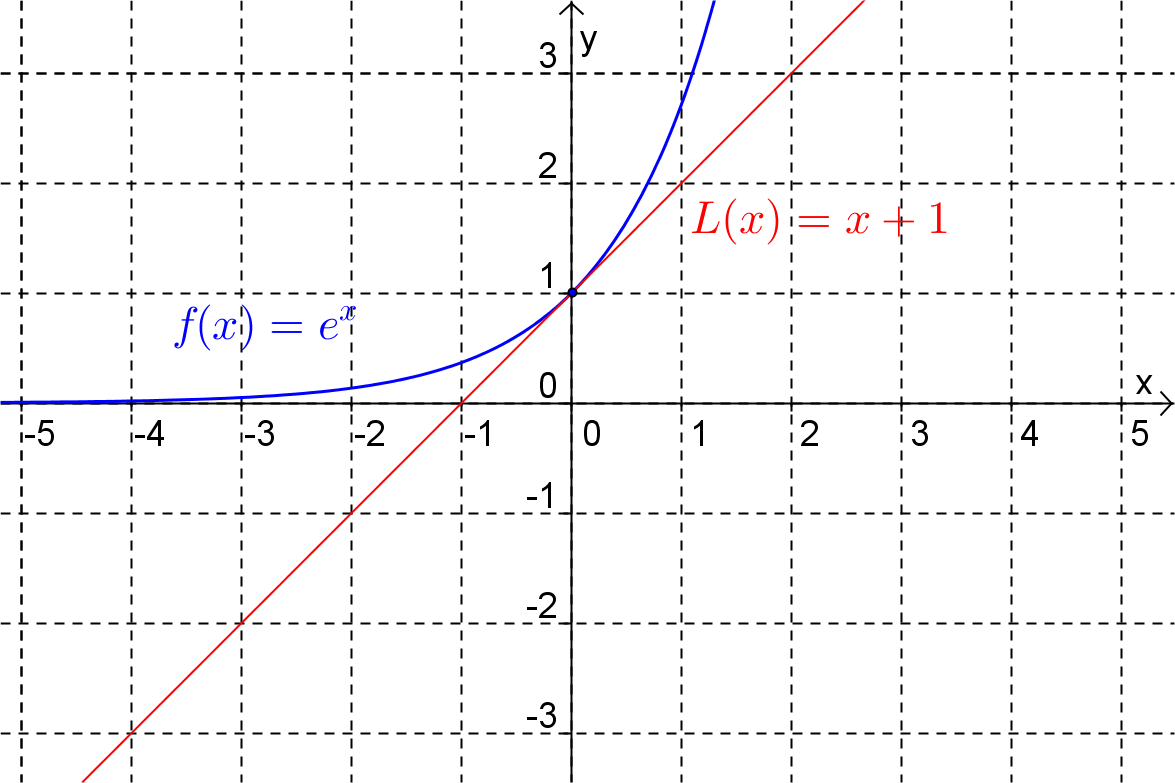
\includegraphics[width=\linewidth]{./Calculus/Images/1/Linear_approximation_of_exponential.png}
\tcblower
\end{figureptx}%
\end{sbspanel}%
\begin{sbspanel}{0.45}%
\begin{figureptx}{}{x:figure:Fig-Quadratic_approximation_of_exponential}{}%
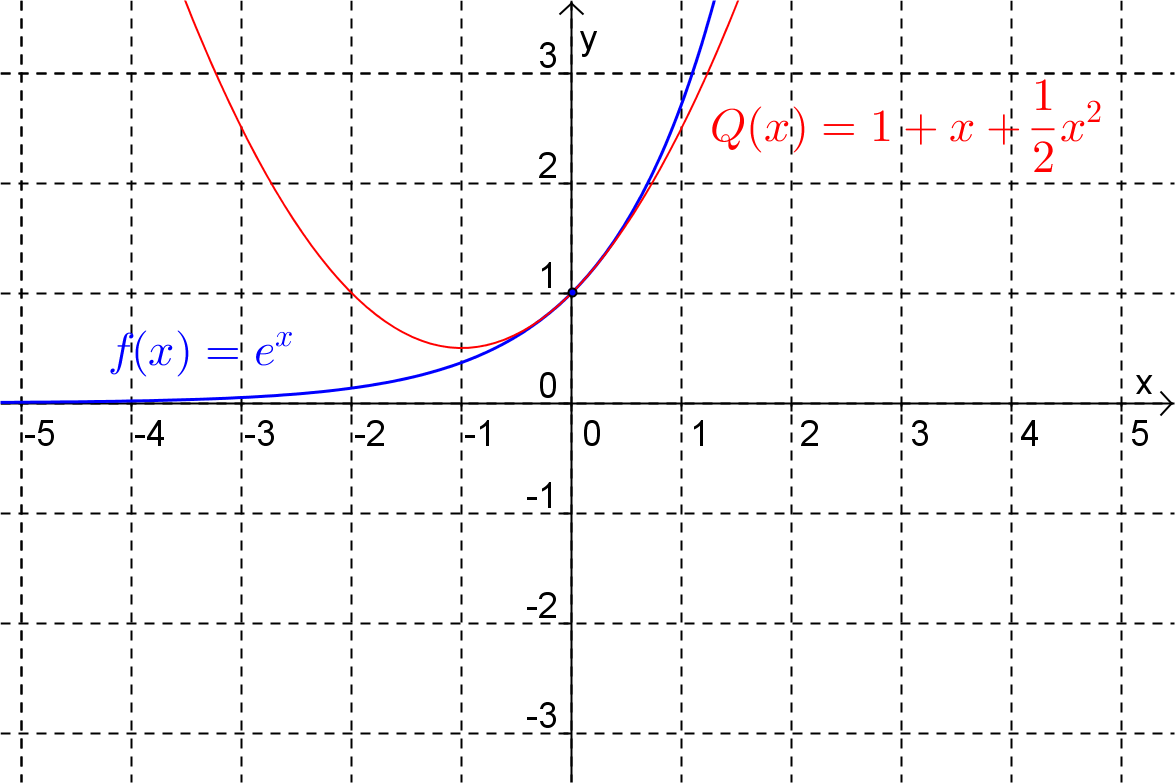
\includegraphics[width=\linewidth]{./Calculus/Images/1/Quadratic_approximation_of_exponential.png}
\tcblower
\end{figureptx}%
\end{sbspanel}%
\end{sidebyside}%
\par
Notice that the linear approximation, \(L(x)\), is the function obtained by truncating the infinite series representation for \(e^x\) (given above) after two terms. If we were to take the first three terms of the series we would have a quadratic approximation for \(e^x\), i.e.%
\begin{equation*}
Q(x) = 1 + x + \frac{x^2}{2}.
\end{equation*}
%
\par
(See \hyperref[x:figure:Fig-Quadratic_approximation_of_exponential]{Figure~{\xreffont\ref{x:figure:Fig-Quadratic_approximation_of_exponential}}}.) By using more terms from the infinite expansion we can obtain higher order polynomial approximations which we hope will be more accurate over a greater interval around the point of tangency. The idea of approximating a function by a polynomial has many uses in mathematics besides that of being used in calculators.%
\end{sectionptx}
%
%
\typeout{************************************************}
\typeout{Section 1.2 Infinite Series}
\typeout{************************************************}
%
\begin{sectionptx}{Infinite Series}{}{Infinite Series}{}{}{x:section:Sec-Infinite_Series}
In this section we will discuss the concepts and terminology associated with infinite series that we will need in order to discuss representing functions by infinite series.%
\par
An infinite series is a sum of the form%
\begin{equation*}
\sum_{k=1}^{\infty}t_k = t_1 + t_2 +t_3 + \cdots
\end{equation*}
where \(t_k\) are real numbers.%
\par
We call \(t_1, t_1+t_2, t_1+t_2+t_3, \ldots\) the \terminology{sequence} of partial sums for the series.%
\begin{example}{}{x:example:Ex-Sample_infinite_series}%
Both of the following are infinite series:%
\begin{equation*}
\sum_{k=1}^{\infty}\frac{1}{2^k} = \frac{1}{2^1}+\frac{1}{2^2}+\frac{1}{2^3} + \cdots = \frac{1}{2} + \frac{1}{4} + \frac{1}{8} + \cdots 
\end{equation*}
%
\begin{equation*}
\sum_{k=1}^{\infty}(3k+1) = (3\times 0+1)+(3\times 1+1)+(3\times 2+1) + \cdots = 1 + 4 +7 + \cdots.
\end{equation*}
%
\end{example}
The sum of a finite number of real \(x\) numbers is always finite. However, for an infinite sum, as we add more and more terms in the series the sum:%
\begin{itemize}[label=\textbullet]
\item{}Might get closer and closer to some number. This is called \terminology{convergence}. For example%
\begin{equation*}
\sum_{k=1}^{\infty}\frac{1}{2^k}=\frac{1}{2^1}+\frac{1}{2^2}+\frac{1}{2^3}+\cdots = \frac{1}{2}+\frac{1}{4}+\frac{1}{8}+\cdots.
\end{equation*}
Sometimes a sum reaches a value and does not change (i.e. the terms become zero). We also call this convergence, e.g.%
\begin{equation*}
\sum_{k=1}^{\infty}0 = 0+0+0+\cdots = 0.
\end{equation*}
%
\item{}Any other behaviour is called \terminology{divergence}. For example%
\begin{equation*}
\sum_{k=1}^{\infty}k = 1+2+3+\cdots
\end{equation*}
and%
\begin{equation*}
\sum_{k=1}^{\infty}(-1)^{k-1}=(-1)^0+(-1)^1+(-1)^2+\cdots = 1-1+1-1+1-\cdots
\end{equation*}
(this last example is actually tricky to define properly).%
\end{itemize}
%
\par
On adding the first \(10\) terms of the series \(\displaystyle \sum_{k=1}^{\infty}\frac{1}{2^k}\) we get \(0.99902344\cdots\), on adding the first \(20\) terms we get \(0.99999905\cdots\). So even though as we add more terms the sum is getting larger it is getting closer and closer to some fixed number. Adding lots of terms of the series (as we did above) suggests that for this case the sum is converging to \(1\). If this is the case (and we will show below that it is) then we would say:%
\begin{itemize}[label=\textbullet]
\item{}The series converges to \(1\)%
\item{}The sum of the series is \(1\)%
\item{}The limit of the series is \(1\)%
\end{itemize}
%
\par
There is a lot of mathematics devoted to determining the nature of an infinite series. We will mention just three useful results.%
\begin{theorem}{The Divergence Test.}{}{g:theorem:id542182}%
If the terms \(t_k\) of the series \(\displaystyle \sum_{k=1}^{\infty}t_k\) do not approach \(0\) as \(k\to\infty\) then the series diverges.%
\end{theorem}
\begin{theorem}{Geometric Progressions.}{}{g:theorem:id542164}%
If the infinite series is a geometric progression (GP), i.e., of the form%
\begin{equation*}
\sum_{k=1}^{\infty}ar^k = a +ar +ar^2+ar^3 +\cdots
\end{equation*}
then it converges if and only if \(|r|< 1\), in which case it converges to%
\begin{equation*}
S=\frac{a}{1-r}.
\end{equation*}
%
\end{theorem}
\begin{theorem}{The Ratio Test.}{}{g:theorem:id542207}%
For the series \(\displaystyle \sum_{k=1}^{\infty}t_k\), let \(\displaystyle L=\lim_{k\to \infty}\left|\dfrac{t_{k+1}}{t_k}\right|\). If%
\begin{itemize}[label=\textbullet]
\item{}\(L<1\) then the series converges%
\item{}\(L>1\) then the series diverges%
\item{}\(L=1\) then the test is inconclusive%
\end{itemize}
%
\end{theorem}
\begin{example}{}{x:example:Ex-Divergence_test}%
Determine the nature of the series  \(\displaystyle\sum_{k=1}^{\infty}k = 1+2+3+\cdots.\)%
\par\smallskip%
\noindent\textbf{\blocktitlefont Answer}.\hypertarget{g:answer:id542241}{}\quad{}Divergent.%
\par\smallskip%
\noindent\textbf{\blocktitlefont Solution}.\hypertarget{g:solution:id542265}{}\quad{}Since the terms of the series do not approach 0 as we go along the series, by the Divergence Test, this series diverges.%
\end{example}
\begin{example}{}{x:example:Ex-Geometric_progression}%
Determine the nature of the series%
\begin{equation*}
\sum_{k=1}^{\infty}\frac{1}{2^k} = \dfrac{1}{2}+\dfrac{1}{4}+\dfrac{1}{8}+\cdots.
\end{equation*}
%
\par\smallskip%
\noindent\textbf{\blocktitlefont Answer}.\hypertarget{g:answer:id542254}{}\quad{}Convergent.%
\par\smallskip%
\noindent\textbf{\blocktitlefont Solution}.\hypertarget{g:solution:id542273}{}\quad{}This infinite series is a GP with \(a=\dfrac{1}{2}\) and \(r=\dfrac{1}{2}\). Since \(|r|<1\) the series converges and converges to%
\begin{equation*}
S=\dfrac{1/2}{1-1/2} =1.
\end{equation*}
%
\end{example}
\begin{example}{}{x:example:Ex-Ratio_test}%
Determine the nature of the series%
\begin{equation*}
\sum_{k=1}^{\infty}\frac{k+1}{2^k} = 1+\dfrac{3}{4}+\dfrac{1}{2}+\dfrac{5}{16}+\cdots.
\end{equation*}
%
\par\smallskip%
\noindent\textbf{\blocktitlefont Answer}.\hypertarget{g:answer:id542314}{}\quad{}Convergent.%
\par\smallskip%
\noindent\textbf{\blocktitlefont Solution}.\hypertarget{g:solution:id542292}{}\quad{}To use the ratio test consider%
\begin{equation*}
\dfrac{t_{k+1}}{t_k} = \dfrac{k+2}{2^{k+1}}\cdot\dfrac{2^k}{k+1} = \dfrac{1}{2}\left(\dfrac{k+2}{k+1}\right).
\end{equation*}
%
\par
Thus%
\begin{equation*}
L=\lim_{k\to\infty}\left|\dfrac{1}{2}\left(\dfrac{k+2}{k+1}\right)\right|=\dfrac{1}{2}.
\end{equation*}
%
\par
Since \(L<1\), by the ratio test this series converges. (Notice that the ratio test doesn't tell us to what number the series converges to. In this case it is 3.)%
\end{example}
We eventually want to represent a function via an infinite series. To do so the infinite series will have to involve a variable (the independent variable of the function). Clearly for an infinite series involving a variable the behaviour of the series will depend upon the value of the variable.%
\begin{example}{}{x:example:Ex-Power_series_motivation}%
For which values of \(x\) will the following series converge?%
\begin{equation*}
\sum_{k=0}^{\infty}\left(\dfrac{-2x}{3}\right)^k = 1-\dfrac{2}{3}x + \dfrac{4}{9}x^2 -\dfrac{8}{27}x^3 + \cdots.
\end{equation*}
%
\par\smallskip%
\noindent\textbf{\blocktitlefont Answer}.\hypertarget{g:answer:id542319}{}\quad{}\(-\dfrac{3}{2} < x < \dfrac{3}{2}\).%
\par\smallskip%
\noindent\textbf{\blocktitlefont Solution}.\hypertarget{g:solution:id542340}{}\quad{}Note that this is a GP with \(a=1\) and \(r=\dfrac{-2x}{3}\). Thus the series will only converge for those values of \(x\) that satisfy \(\left|\dfrac{-2x}{3}\right| < 1 \), that is, \(-\dfrac{3}{2} < x < \dfrac{3}{2}\).%
\par
Just to check this, let \(x=1\). Then the series becomes%
\begin{equation*}
\sum_{k=0}^{\infty}\left(\dfrac{-2}{3}\right)^k = 1-\dfrac{2}{3} + \dfrac{4}{9} -\dfrac{8}{27} + \cdots
\end{equation*}
which converges to \(S=\dfrac{1}{1+2/3}=\dfrac{3}{5}\). Note that, on adding the first \(20\) terms of the series we get \(0.59981956\cdots\) and on adding the first \(50\) terms we get \(0.59999991\cdots\), and so it does indeed seem that the sum is \(3/5\).%
\end{example}
\begin{definition}{Power Series.}{g:definition:id542363}%
A \terminology{power series} about \(a\) is an infinite series of the form%
\begin{equation*}
\sum_{k=0}^{\infty}c_k(x-a)^k = c_0 + c_1(x-a) + c_2(x-a)^2 + c_3(x-a)^3 + \cdots
\end{equation*}
where the \(c_k\) are real numbers.%
\end{definition}
\begin{example}{}{x:example:Ex-Power_series_geometric}%
The series%
\begin{equation*}
\sum_{k=0}^{\infty}x^k = 1+x+x^2+x^3+\cdots
\end{equation*}
is a power series about \(0\) (with \(c_k=1\) for all \(k\)). There are several points worth noting about this power series.%
\begin{itemize}[label=\textbullet]
\item{}The series definitely converges when \(x = 0\).%
\item{}The series is a GP with \(a=1\) and \(r=x\) and so converges for \(|x|<1\).%
\item{}When the series converges it converges to \(S=\dfrac{1}{1-x}\).%
\end{itemize}
This last point is interesting because it is telling us that for \(f(x)=\dfrac{1}{1-x}\) if \(|x|<1\) we have%
\begin{equation*}
f(x)=\sum_{k=0}^{\infty}x^k.
\end{equation*}
%
\end{example}
\begin{example}{}{x:example:Ex-Power_series_ratio_test}%
The series%
\begin{equation*}
\sum_{k=0}^{\infty}\dfrac{(x-1)^k}{k+1} = 1+\dfrac{x-1}{2}+\dfrac{(x-1)^2}{3}+\cdots
\end{equation*}
is a power series about \(1\). For this series%
\begin{itemize}[label=\textbullet]
\item{}It definitely converges for \(x = 1\).%
\item{}It can be shown, via the ratio test, that the series converges for \(0 < x <2\). Firstly,%
\begin{equation*}
L =\lim_{k\to\infty}\left|\dfrac{(x-1)^{k+1}}{k+2}\cdot\dfrac{k+1}{(x-1)^k}\right| = |x-1|.
\end{equation*}
Thus \(L<1\) when \(|x-1|<1\), i.e., \(0 < x <2\).%
\par
For example, with \(x=3/2\) adding the first \(20\) terms gives \(1.3862947\cdots\) while adding the first \(50\) terms gives \(1.3862943\cdots\).%
\item{}For \(0 < x <2\) we can think of this infinite series as defining a function, i.e.%
\begin{equation*}
f(x) = \sum_{k=0}^{\infty}\dfrac{(x-1)^k}{k+1}.
\end{equation*}
In which case, as we saw above, \(f(3/2)=1.3863\) to \(4\) d.p.%
\end{itemize}
%
\end{example}
\begin{remark}{}{g:remark:id542576}%
Note that it can be shown that a power series about \(x=a\) either%
\begin{itemize}[label=\textbullet]
\item{}Converges only for \(x=a\)%
\item{}Converges for \(|x-a|<R\) and diverges for \(|x-a|>R\) (note what happens when \(|x-a|=R\) depends on the particular power series)%
\item{}Converges for all \(x\)%
\end{itemize}
The value of \(R\) is called the \terminology{radius of convergence}. In the first case we say \(R=0\) and in the third case we say \(R=\infty\). The collection of those \(x\) for which the series converges is called the \terminology{interval of convergence} \(I\) of the power series.%
\end{remark}
%
%
\typeout{************************************************}
\typeout{Exercises 1.2 Example Tasks}
\typeout{************************************************}
%
\begin{exercises-subsection-numberless}{Example Tasks}{}{Example Tasks}{}{}{g:exercises:id542584}
\begin{divisionexercise}{1}{}{}{g:exercise:id542590}%
Determine whether the following series converge or diverge. If the series is a convergent GP then find its sum.%
\begin{multicols}{2}
\begin{enumerate}[label=\alph*]
\item{}\(\displaystyle \displaystyle \sum_{k=0}^{\infty}\dfrac{1}{3+2^{-k}}\)%
\item{}\(\displaystyle \displaystyle \sum_{k=1}^{\infty}\dfrac{3}{10^{k}}\)%
\item{}\(\displaystyle \displaystyle \sum_{k=1}^{\infty}\dfrac{k^3}{3^k}\)%
\item{}\(\displaystyle \displaystyle \sum_{k=1}^{\infty}\dfrac{k}{k^2+4}\)%
\end{enumerate}
\end{multicols}
%
\end{divisionexercise}%
\begin{divisionexercise}{2}{}{}{g:exercise:id542624}%
Determine the interval of convergence for the following series.%
\begin{multicols}{2}
\begin{enumerate}[label=\alph*]
\item{}\(\displaystyle \displaystyle \sum_{k=1}^{\infty}\dfrac{(3x-2)^k}{k3^k}\)%
\item{}\(\displaystyle \displaystyle \sum_{k=1}^{\infty}(-1)^k\dfrac{x^{2k}}{(2k)!}\)%
\end{enumerate}
\end{multicols}
%
\end{divisionexercise}%
\end{exercises-subsection-numberless}
\begin{remark}{Aside.}{g:remark:id542643}%
Computer algebra systems usually have commands for summing infinite series. For example, with Wolfram Alpha you can just type in the first few terms as shown.%
\begin{figureptx}{}{x:figure:Fig-C1_WA_1}{}%
\begin{image}{0.05}{0.9}{0.05}%
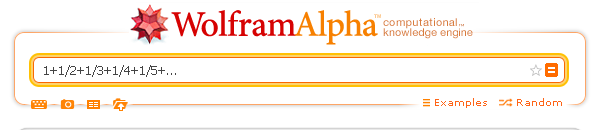
\includegraphics[width=\linewidth]{./Calculus/Images/1/C1_WA_1.png}
\end{image}%
\tcblower
\end{figureptx}%
\begin{figureptx}{}{x:figure:Fig-C1_WA_2}{}%
\begin{image}{0.05}{0.9}{0.05}%
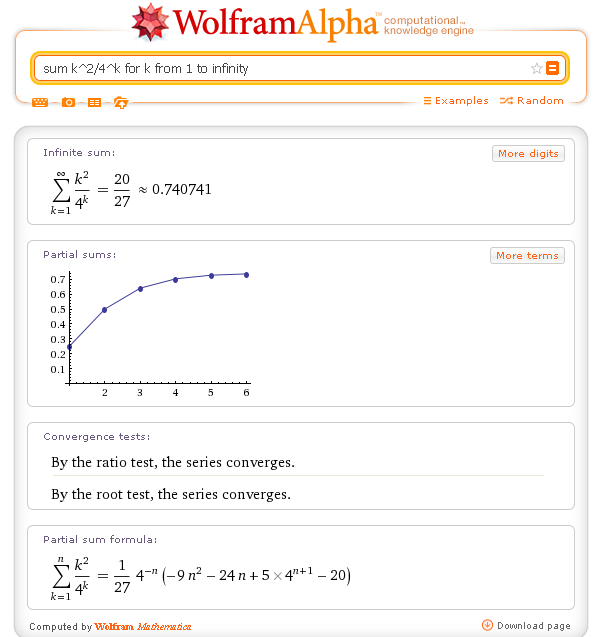
\includegraphics[width=\linewidth]{./Calculus/Images/1/C1_WA_2.png}
\end{image}%
\tcblower
\end{figureptx}%
\end{remark}
\end{sectionptx}
%
%
\typeout{************************************************}
\typeout{Section 1.3 Maclaurin Series}
\typeout{************************************************}
%
\begin{sectionptx}{Maclaurin Series}{}{Maclaurin Series}{}{}{x:section:Sec-Maclaurin_Series}
In this section we will discuss the task of finding an infinite series representation for a given function of one variable, \(f\). We begin by assuming that the given function \(f(x)\) does indeed have a power series representation, at least initially about \(x=0\). Thus we assume that on some interval \(|x| < R\)%
\begin{equation}
f(x) = \sum_{k=0}^{\infty}c_kx^k = c_0 + c_1x +c_2x^2 +c_3x^3 + \cdots.\label{x:men:Eq-Maclaurin_of_f}
\end{equation}
%
\par
We know that the power series reduces to \(c_0\) when \(x=0\) and so for the power series to match the function when \(x=0\) we must have \(c_0 = f(0)\). On differentiating \hyperref[x:men:Eq-Maclaurin_of_f]{({\xreffont\ref{x:men:Eq-Maclaurin_of_f}})} we get%
\begin{equation}
f'(x) = \sum_{k=1}^{\infty}kc_kx^{k-1} = c_1 +2c_2x +3c_3x^2 + 4c_4x^3 + \cdots\label{x:men:Eq-First_derivative_Maclaurin}
\end{equation}
and putting on \(x=0\) into this gives \(c_1=f'(0)\). Similarly, differentiating \hyperref[x:men:Eq-First_derivative_Maclaurin]{({\xreffont\ref{x:men:Eq-First_derivative_Maclaurin}})}%
\begin{equation}
f''(x) = \sum_{k=2}^{\infty}k(k-1)c_kx^{k-2} = 2c_2 +6c_3x + 12c_4x^2 + \cdots\label{g:men:id542751}
\end{equation}
and substituting \(x=0\) gives \(c_2=\dfrac{1}{2}f''(0)\). By continuing this process, we can see that in general%
\begin{equation}
f^{(n)}(x) = \sum_{k=n}^{\infty}k(k-1)(k-2)\cdots(k-(n-1))c_kx^{k-n}\label{g:men:id542750}
\end{equation}
and hence (by substituting \(x=0\)) that \(c_n = \dfrac{1}{n!}f^{(n)}(0)\).%
\begin{definition}{Maclaurin Series.}{g:definition:id542742}%
The series%
\begin{equation*}
\sum_{k=0}^{\infty}\dfrac{f^{(k)}(0)}{k!}x^k = f(0) + f'(0)x +\dfrac{f^{''}(0)}{2!}x^2 +\dfrac{f^{'''}(0)}{3!}x^3 + \cdots
\end{equation*}
is called the \terminology{Maclaurin series} for \(f(x)\).%
\end{definition}
We know that the Maclaurin series for \(f\) converges when \(x=0\) (since all power series converge for \(f(x)\)) and we also know that the series converges to \(f(0)\) (because we constructed it that way). However for other values of \(x\) we cannot be sure that the infinite series will converge and if it does, does it converge to the function value.%
\begin{example}{}{x:example:Ex-Maclaurin_series_geometric}%
Find the Maclaurin series for \(f(x)=\dfrac{1}{1-x}\).%
\par\smallskip%
\noindent\textbf{\blocktitlefont Answer}.\hypertarget{g:answer:id542812}{}\quad{}\(\displaystyle \sum_{k=0}^{\infty}x^k = 1+x+x^2+x^3+x^4+ \cdots\)%
\par\smallskip%
\noindent\textbf{\blocktitlefont Solution}.\hypertarget{g:solution:id542841}{}\quad{}Firstly find the derivatives of \(f\) and evaluate them at \(x=0\).%
\begin{alignat*}{1}
f(x) \amp = (1-x)^{-1} \text{ and hence } f(0)=1\\
f'(x) \amp = (1-x)^{-2} \text{ and hence } f'(0)=1\\
f''(x) \amp = 2(1-x)^{-3} \text{ and hence } f''(0)=2\\
\quad\amp \vdots \quad \\
f^{(k)}(x) \amp = k!(1-x)^{-k-1} \text{ and hence } f^{(k)}(0) = k!
\end{alignat*}
Substituting these results into the formula derived above gives the Maclaurin series for \(f\) as%
\begin{equation*}
\sum_{k=0}^{\infty}\dfrac{k!}{k!}x^k = 1+x+x^2+x^3+x^4+ \cdots.
\end{equation*}
This agrees with the result that we found in an earlier example. As we saw in that example, however, the Maclaurin series only converges for \(|x| <1 \) and that for those values it converges to the function value.%
\end{example}
\begin{definition}{Maclaurin Polynomial.}{g:definition:id542860}%
The \(n\)th partial sum of the Maclaurin series for \(f(x)\), i.e.,%
\begin{equation*}
\sum_{k=0}^{n}\dfrac{f^{(k)}(0)}{k!}x^k = f(0) + f'(0)x +\dfrac{f^{''}(0)}{2!}x^2 +\cdots + \dfrac{f^{(n)}(0)}{n!}x^n 
\end{equation*}
is called the \terminology{Maclaurin polynomial of degree \(n\)} for \(f(x)\).%
\end{definition}
\begin{example}{}{x:example:Ex-Maclaurin_polynomial_cosine}%
Find the Maclaurin polynomials of degree \(0,1,2,3\) and \(4\) for the function \(f(x)=\cos(x)\).%
\par\smallskip%
\noindent\textbf{\blocktitlefont Answer}.\hypertarget{g:answer:id542920}{}\quad{}\(M_0(x)=1\)%
\par
\(M_1(x)=1\)%
\par
\(M_2(x)=1-\dfrac{x^2}{2}\)%
\par
\(M_3(x)=1-\dfrac{x^2}{2}\)%
\par
\(M_4(x)=1-\dfrac{x^2}{2}+\dfrac{x^4}{24}\)%
\par\smallskip%
\noindent\textbf{\blocktitlefont Solution}.\hypertarget{g:solution:id542897}{}\quad{}For \(f(x)=\cos(x)\),%
\begin{alignat*}{1}
f(x) \amp = \cos(x) \text{ and hence } f(0)=1\\
f'(x) \amp = -\sin(x) \text{ and hence } f'(0)=0\\
f''(x) \amp = -\cos(x) \text{ and hence } f''(0)=-1\\
f'''(x) \amp = \sin(x) \text{ and hence } f'''(0)=0\\
f^{(iv)}(x) \amp = \cos(x) \text{ and hence } f^{(iv)}(0)=1
\end{alignat*}
and so the \(0\)th degree Maclaurin polynomial is%
\begin{equation*}
M_0(x)=f(0)=1.
\end{equation*}
Notice that the \(0\)th degree Maclaurin polynomial is the horizontal line passing through the point \((0,f(0))\).%
\par
The \(1\)st degree Maclaurin polynomial is%
\begin{alignat*}{1}
M_1(x) \amp = f(0) + f'(0)x\\
\amp = 1+0\\
\amp = 1
\end{alignat*}
Notice that the \(1\)st degree Maclaurin polynomial is the tangent to the function at the point  \((0,f(0))\). Notice also, that in this case, the \(0\)th degree and the \(1\)st  degree Maclaurin polynomials are the same.%
\par
The \(2\)nd degree Maclaurin polynomial is%
\begin{alignat*}{1}
M_2(x) \amp = f(0) + f'(0)x + \dfrac{f''(0)}{2}x^2\\
\amp = 1+0x + \dfrac{(-1)}{2}x^2\\
\amp = 1-\dfrac{x^2}{2}
\end{alignat*}
%
\par
The \(3\)rd degree Maclaurin polynomial is%
\begin{alignat*}{1}
M_3(x)  \amp = f(0) + f'(0)x + \dfrac{f''(0)}{2}x^2 + \dfrac{f'''(0)}{3!}x^3\\
\amp = 1+0x + \dfrac{(-1)}{2}x^2 + \dfrac{0}{3!}x^3\\
\amp = 1-\dfrac{x^2}{2}
\end{alignat*}
%
\par
The \(4\)th degree Maclaurin polynomial is%
\begin{alignat*}{1}
M_4(x)  \amp = f(0) + f'(0)x + \dfrac{f''(0)}{2}x^2 + \dfrac{f'''(0)}{3!}x^3 + \dfrac{f^{(iv)}(0)}{4!}x^4\\
\amp = 1+0x + \dfrac{(-1)}{2}x^2 + \dfrac{0}{3!}x^3 + \dfrac{1}{4!}x^4\\
\amp = 1-\dfrac{x^2}{2} + \dfrac{x^4}{24}
\end{alignat*}
As can be seen in \hyperref[x:figure:Fig-Maclaurin_polynomial_cosine]{Figure~{\xreffont\ref{x:figure:Fig-Maclaurin_polynomial_cosine}}}, in this case as the degree of the Maclaurin polynomial increases so the polynomial provides a good approximation to the function for a larger interval surrounding \(x=0\). In fact, using the Ratio test we can show that the Maclaurin series for \(\cos(x)\) converges for all values of \(x\) and by using some more advanced mathematics we can show that the series converges to \(\cos(x)\) for all values of \(x\).%
\begin{figureptx}{}{x:figure:Fig-Maclaurin_polynomial_cosine}{}%
\begin{image}{0.05}{0.9}{0.05}%
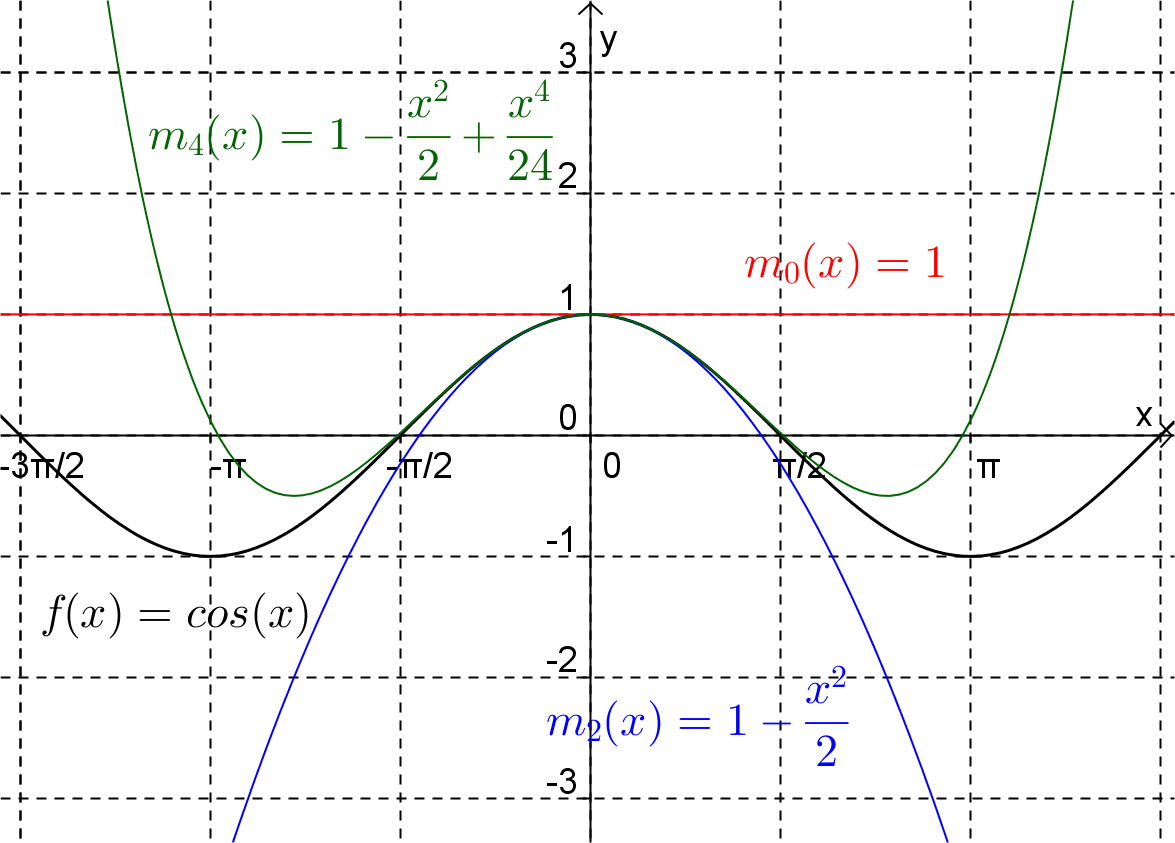
\includegraphics[width=\linewidth]{./Calculus/Images/1/Fig-Maclaurin_polynomial_cosine.png}
\end{image}%
\tcblower
\end{figureptx}%
\end{example}
%
%
\typeout{************************************************}
\typeout{Exercises 1.3 Example Tasks}
\typeout{************************************************}
%
\begin{exercises-subsection-numberless}{Example Tasks}{}{Example Tasks}{}{}{g:exercises:id543053}
\begin{divisionexercise}{1}{}{}{g:exercise:id543077}%
Let \(f(x)=e^x\). Find the Maclaurin series for \(f\) and find its interval of convergence.\end{divisionexercise}%
\begin{divisionexercise}{2}{}{}{g:exercise:id543081}%
Find the Maclaurin polynomial of degree \(3\) for \(g(x) = \tan^{-1}(x)\).\end{divisionexercise}%
\end{exercises-subsection-numberless}
\begin{remark}{Aside.}{g:remark:id543119}%
Computer Algebra Systems usually have a command for calculating Maclaurin series. For example, the following shows part of the output from a Wolfram Alpha query.%
\begin{figureptx}{}{x:figure:Fig-C1_WA_3}{}%
\begin{image}{0.05}{0.9}{0.05}%
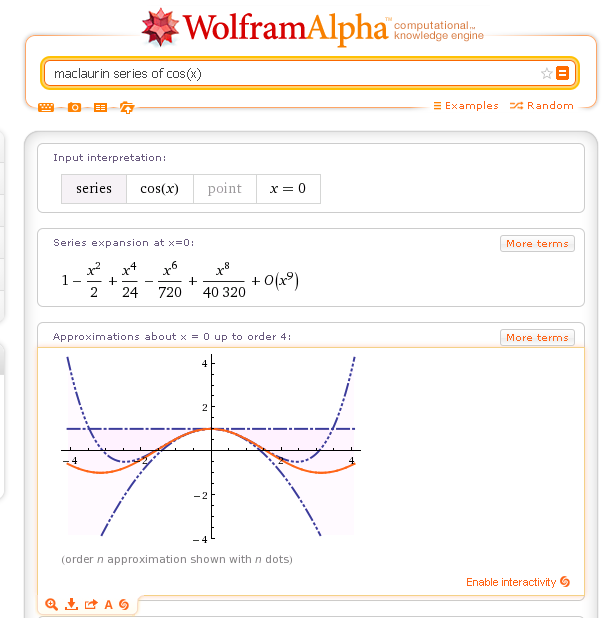
\includegraphics[width=\linewidth]{./Calculus/Images/1/C1_WA_3.png}
\end{image}%
\tcblower
\end{figureptx}%
\end{remark}
\end{sectionptx}
\end{chapterptx}
 %
%
\typeout{************************************************}
\typeout{Chapter 2 Taylor Series}
\typeout{************************************************}
%
\begin{chapterptx}{Taylor Series}{}{Taylor Series}{}{}{x:chapter:Calculus_2}
%
%
\typeout{************************************************}
\typeout{Section 2.1 Generating New Series from Known Series}
\typeout{************************************************}
%
\begin{sectionptx}{Generating New Series from Known Series}{}{Generating New Series from Known Series}{}{}{x:section:Generating-New-Series-from-Known-Series}
In Table \(1\) below we have listed the Maclaurin series for a small set of basic functions of science and engineering. These series can all be relatively easily derived from first principals as discussed in previous lectures. However, for some more complex functions it is easier to find their Maclaurin series by starting from known series rather than trying to find the series from scratch. We will look at two commonly used techniques.%
\par
%
\begin{enumerate}
\item{}Manipulating\slash{}Substituting into known series.%
\item{}Differentiating\slash{}Integrating known series.%
\end{enumerate}
%
\par
%
\par
%
\begin{enumerate}
\item{}\(\displaystyle \dfrac{1}{1-x}=\sum_{k=0}^{\infty}x^{k}=1+x+x^{2}+x^{3}+\cdots . \hspace{5cm}  \lvert x\rvert < 1  \)%
\item{}\(\displaystyle e^{x}=\sum_{k=0}^{\infty}\dfrac{x^{k}}{k!}=1+x+\dfrac{x^{2}}{2!} +\dfrac{x^{3}}{3!}+\cdots .  \hspace{5.6cm}\sim \)%
\item{}\(\displaystyle \sin(x)=\sum_{k=0}^{\infty}(-1)^{k}\dfrac{x^{2k+1}}{(2k+1)!}=x-\dfrac{x^{3}}{3!} +\dfrac{x^{5}}{5!}-\cdots .\hspace{3cm}\sim \)%
\item{}\(\displaystyle \cos(x)=\sum_{k=0}^{\infty}(-1)^{k}\dfrac{x^{2k}}{(2k)!}=1-\dfrac{x^{2}}{2!} +\dfrac{x^{4}}{4!}-\cdots .\hspace{3.9cm} \sim \)%
\item{}\(\displaystyle \ln(1+x)=\sum_{k=0}^{\infty}(-1)^{k-1}\dfrac{x^{k}}{(k)}=x-\dfrac{x^{2}}{2} +\dfrac{x^{3}}{3}-\cdots . \hspace{2.5cm}  \lvert x\rvert < 1 \)%
\item{}\(\displaystyle \tan^{-1}(1+x)=\sum_{k=0}^{\infty}(-1)^{k}\dfrac{x^{2k+1}}{(2k+1)}=x-\dfrac{x^{3}}{3} +\dfrac{x^{5}}{5}-\cdots . \hspace{1.1cm} \lvert x\rvert < 1 \)%
\item{}\(\displaystyle \sinh(x)=\sum_{k=0}^{\infty}\dfrac{x^{2k+1}}{(2k+1)!}=x+\dfrac{x^{3}}{3!} +\dfrac{x^{5}}{5!}+\cdots . \hspace{3.9cm} \sim \)%
\item{}\(\displaystyle \cosh(x)=\sum_{k=0}^{\infty}\dfrac{x^{2k}}{(2k)!}=1+\dfrac{x^{2}}{2!} +\dfrac{x^{4}}{4!}+\cdots . \hspace{4.8cm} \sim \)%
\end{enumerate}
%
\begin{paragraphs}{Manipulating\slash{}Substituting into Known Series.}{g:paragraphs:id543248}%
\end{paragraphs}%
\begin{example}{}{x:example:Maclaurin_series_1_on_1_plus_x2}%
Find the Maclaurin series for  \(f(x)=\dfrac{1}{1+x^{2}}. \)%
\par\smallskip%
\noindent\hypertarget{g:solution:id543292}{}We know that the Maclaurin series for\(f(x)=\dfrac{1}{1-x}\) on \(\lvert x\rvert < 1 \) is%
%
\begin{equation*}
\dfrac{1}{1-x}=\sum_{k=0}^{\infty}x^{k}=1+x+x^{2}+x^{3}+\cdots \cdot 
\end{equation*}
We can use this series by replacing \(x \) with \(-x^{2} \) to obtain%
\par
%
\begin{align*}
\dfrac{1}{1+x^{2}} \amp =\dfrac{1}{1-(-x^{2})}\\
\amp = 1+(-x^{2})+(-x^{2})^{2}+(-x^{2})^{3}+\cdots\\
\amp = 1-\dfrac{x^{2}}{2!} +\dfrac{x^{4}}{4!}-\cdots\\
\amp = \sum_{k=0}^{\infty}(-1)^{k}x^{2k}
\end{align*}
%
\par
which will converge on the interval \(\lvert -x^{2}\rvert < 1, \) i.e., \(-1< x < 1. \)%
\end{example}
\begin{example}{}{x:example:Maclaurin_series_x_on_2_minus_5x}%
Find the Maclaurin series for  \(f(x)=\dfrac{1}{1+x^{2}}. \)%
\par\smallskip%
\noindent\hypertarget{g:solution:id543344}{}Once again we will use the Maclaurin series for \(f(x)=\dfrac{1}{1-x}\) on \(\lvert x\rvert < 1. \) Now%
\par
%
\begin{align*}
\frac{x^2}{2-5x} \amp =\dfrac{x^{2}}{2}(\dfrac{1}{1-(\frac{5x}{2})})\\
\amp = \dfrac{x^2}{2}(1+(\frac{5x}{2})+(\frac{5x}{2})^{2}+(\frac{5x}{2})^{3}+\cdots)\\
\amp = \dfrac{x^2}{2}\sum_{k=0}^{\infty}(\dfrac{5x}{2})^{k}
\end{align*}
%
\par
which will converge on the interval \(\lvert \frac{5x}{2}\rvert < 1, \) i.e., \(-\frac{2}{5}< x < \frac{2}{5}. \)%
\end{example}
\begin{example}{}{x:example:Maclaurin_series_e_minus_x_2}%
Find the Maclaurin series for  \(f(x)=e^{-x^2}. \)%
\par\smallskip%
\noindent\hypertarget{g:solution:id543378}{}Substituting into the Maclaurin series for  \(f(x)=e^{x}\) .%
\par
%
\begin{align*}
e^{-x^2} \amp =\sum_{k=0}^{\infty}\dfrac{(-x^2)^{k}}{k!}=\sum_{k=0}^{\infty}(-1)^{k}\dfrac{(x)^{2k}}{k!}\\
\amp = 1- x^{2}+\frac{x^{4}}{2!}-\frac{x^{6}}{3!}+\cdots
\end{align*}
%
\par
which will converge for all real values of \(x. \)%
\end{example}
\begin{paragraphs}{Differentiating\slash{}Integrating Known Series.}{g:paragraphs:id543416}%
\end{paragraphs}%
\par
As the theorem below says, we can also use differentiation and integration to work out new Maclaurin series expansions from ones that we already know. The proof of this theorem is beyond the scope of this course.%
\begin{theorem}{}{}{g:theorem:id543393}%
If  \(f(x)=\sum\limits_{k=0}^{\infty}c_{k}x^{k}\) with radius of convergence \(\mathbb{R} \) then%
\par
%
\begin{enumerate}[label=\roman*]
\item{}\(f'(x)=\sum\limits_{k=0}^{\infty}k c_{k}x^{k-1}\) with radius of convergence   \(\mathbb{R}, \)%
\item{}\(\int f(x)dx=K+ \sum\limits_{k=0}^{\infty} \dfrac{c_{k}}{k+1}x^{k-1}\) with radius of convergence   \(\mathbb{R}, \) (where \(K \)  is a constant).%
\end{enumerate}
%
\end{theorem}
Note that the behaviour of the series (i.e. whether it converges or diverges) at the endpoints may change when it is differentiated or integrated.%
\begin{example}{}{x:example:Maclaurin_series_1_on_1_minus_x_power_2}%
Find the Maclaurin series for  \(ff(x)=\dfrac{1}{(1-x)^{2}}.\)%
\par\smallskip%
\noindent\hypertarget{g:solution:id543459}{}Notice that \(\int \frac{1}{(1-x)^{2}}=\frac{1}{1-x}, \) or put the other way, \(\frac{1}{(1-x)^{2}}=\frac{d}{dx} (\frac{1}{1-x}). \) Since we know the Maclaurin series for \(\frac{1}{1-x} \) we can differentiate this series to obtain the Maclaurin series for \(\frac{1}{(1-x)^{2}}. \) So, on \(\lvert x\rvert < 1, \)%
\par
%
\begin{align*}
\frac{1}{(1-x)^{2}} \amp =\frac{d}{dx}(\sum_{k=0}^{\infty} x^{k})\\
\amp = \frac{d}{dx}(\sum_{k=1}^{\infty} k x^{k-1}\\
\amp = 1+2x+3x^2+4x^3+\dots 
\end{align*}
%
\end{example}
\begin{example}{}{x:example:Maclaurin_series_ln_1_plus_x}%
Find the Maclaurin series for  \(ff(x)=\ln(1+x).\)%
\par\smallskip%
\noindent\hypertarget{g:solution:id543494}{}Notice that \(\frac{d}{(dx)}(\ln(1+x)), \) or put the other way, \(\ln(1+x)=K+\int \frac{1}{1+x}. \) Since we know the Maclaurin series for \(\frac{1}{1+x} \) we can integrate this series to obtain the Maclaurin series for \(\ln(1+x).\) So, on \(\lvert x\rvert < 1, \)%
\par
%
\begin{align*}
\ln(1+x) \amp = K+\int (\sum_{k=0}^{\infty} (-x)^{k})dx\\
\amp = K+\sum_{k=0}^{\infty} (-1)^{k}\frac{x^{k+1}}{k+1}\\
\amp = K + x - \frac{1}{2}x^{2} +\frac{1}{3}x^{3} - \dots
\end{align*}
%
\par
Since \(\ln(1+x)\) is \(0 \) when \(x=0 \) we have \(K=0. \) Thus on \(\lvert x\rvert < 1 \)%
%
\begin{equation*}
\ln(1+x)=\sum_{k=0}^{\infty}(-1)^{k-1}\frac{x^{k}}{k}=x-\frac{x^{2}}{2}+\frac{x^{3}}{3}-\cdots \cdot 
\end{equation*}
\end{example}
%
%
\typeout{************************************************}
\typeout{Exercises 2.1 Example Tasks}
\typeout{************************************************}
%
\begin{exercises-subsection-numberless}{Example Tasks}{}{Example Tasks}{}{}{g:exercises:id543545}
\begin{divisionexercise}{1}{}{}{g:exercise:id543551}%
Find the Maclaurin series for  \(f(x)=\frac{1}{3+2x}. \)%
\end{divisionexercise}%
\begin{divisionexercise}{2}{}{}{g:exercise:id543548}%
Find the Maclaurin series for  \(f(x)=\frac{1-x^2}{5-3x^2}. \)%
\end{divisionexercise}%
\begin{divisionexercise}{3}{}{}{g:exercise:id543554}%
Find the Maclaurin series for \(f(x)=\frac{1}{(1-2x)^2}. \)%
\end{divisionexercise}%
\begin{divisionexercise}{4}{}{}{g:exercise:id543568}%
Find the Maclaurin series for \(f(x)=\tan{-1}(x). \)%
\end{divisionexercise}%
\begin{divisionexercise}{5}{}{}{g:exercise:id543573}%
Use a sixth degree Maclaurin polynomial to estimate  \(f(x)=\int_{0}^{1}e^{-x^{2}}dx. \)%
\end{divisionexercise}%
\end{exercises-subsection-numberless}
\end{sectionptx}
%
%
\typeout{************************************************}
\typeout{Section 2.2 Taylor Series}
\typeout{************************************************}
%
\begin{sectionptx}{Taylor Series}{}{Taylor Series}{}{}{x:section:Taylor_Series}
Maclaurin series are power series about \(x=0. \)  However we can follow exactly the same process to find a power series expansion for a function   \(f(x) \) about any point   \(x=a. \)  We call these power series Taylor Series.%
\begin{definition}{Taylor Series.}{g:definition:id543584}%
The series,%
\par
%
\begin{equation*}
\sum_{k=0}^{\infty}\dfrac{f^{(k)}(a)}{k!}=f(a)+f'(a)(x-a)+\dfrac{f''(a)}{2!}(x-a)^{2}+\dfrac{f'''(a)}{3!}(x-a)^3+ \dots \text{.}
\end{equation*}
%
\par
is called the Taylor series for \(f(x) \) about   \(x=a. \)%
\end{definition}
Note that:%
\par
%
\begin{enumerate}
\item{}We can construct the Taylor series about  \(x=a.  \)  for any function that is infinitely differentiable at  \(x=a.  \)%
\item{}The Taylor series for \(f \) about  \(x=a \)    always converges to  at  \(x=a. \)%
\item{}If the Taylor series converges for other values of \(x \) these will be in an interval centred on \(x=a. \)%
\item{}It is possible that a Taylor series may converge to a value other than the function value.%
\item{}A Maclaurin series is just a Taylor series about  \(x=0.  \)%
\item{}The \(n^{\text{th}} \)  partial sum of the Taylor series for \(f \) about \(x=a \)  is called the \(n^{\text{th}} \) degree Taylor polynomial for\(f \) about  \(x=a. \)%
\end{enumerate}
%
\begin{example}{}{x:example:Taylor_series_cos}%
Find the Taylor series for   \(f(x)=\cos(x) \) about \(x=\frac{\pi}{2} \)%
\par\smallskip%
\noindent\hypertarget{g:solution:id543698}{}In order to find the Taylor series for   \(f(x)=\cos(x) \) about \(x=\frac{\pi}{2} \)   we need to evaluate \(f \) and its derivatives at  \(x=\frac{\pi}{2}. \)  So,%
\par
%
\begin{align*}
f(x) \amp =\cos(x)  \,\, \text{and hence}\,\,   f(\frac{\pi}{2})=0  \\
f'(x) \amp =\sin(x)  \,\, \text{and hence}\,\,   f'(\frac{\pi}{2})=-1 \\
f''(x) \amp =-\cos(x)  \,\, \text{and hence}\,\,   f''(\frac{\pi}{2})=0  \\
f'(x) \amp =-\sin(x)  \,\, \text{and hence}\,\,   f'''(\frac{\pi}{2})=1 \\
\amp \hspace{5.5cm}  \vdots \\
\amp \hspace{4.6cm}  f^{(k)}(\frac{\pi}{2})=\begin{cases} 0 \amp k\;\, \text{even} \\
(-1)^{\frac{k+1}{2}} \amp  k \;\, \text{odd} \end{cases} 
\end{align*}
%
\par
Thus the Taylor series for  \(f(x)=\cos(x) \) about \(x=\frac{\pi}{2} \)  is%
\par
%
\begin{align*}
\amp = 0-(x-\frac{\pi}{2})+0+\frac{1}{3!}(x-\frac{\pi}{2})^{3}-\frac{1}{5!}(x-\frac{\pi}{2})^{5}+\dots\\
\amp =-(x-\frac{\pi}{2})+\frac{(x-\frac{\pi}{2})^{3}}{3!}-\frac{(x-\frac{\pi}{2})^{5}}{5!}+\dots\\
\amp = \sum_{k=1}^{\infty}(-1)^{k}\dfrac{(x-\frac{\pi}{2})^{2k-1}}{(2k-1)!}.
\end{align*}
%
\par
It turns out that this series converges to  \(f(x)=\cos(x) \) for all values of \(x. \)  \hyperref[x:figure:Fig-Taylor_series_cos]{Figure~{\xreffont\ref{x:figure:Fig-Taylor_series_cos}}} shows the graph of \(f(x)=\cos(x) \) and the Taylor polynomials of degree \(1 \)  and degree \(3    \) about \(x=\frac{\pi}{2} .\)%
\begin{figureptx}{}{x:figure:Fig-Taylor_series_cos}{}%
\begin{image}{0.075}{0.85}{0.075}%
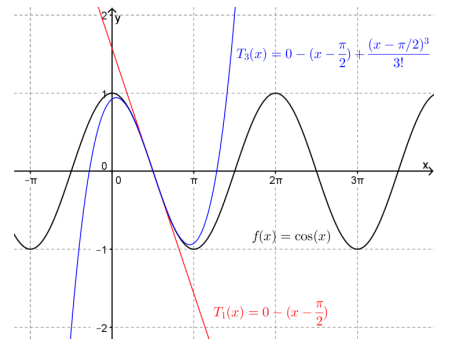
\includegraphics[width=\linewidth]{./Calculus/Images/2/Taylor_series_cos.png}
\end{image}%
\tcblower
\end{figureptx}%
\end{example}
\begin{example}{}{x:example:Second_order_approximation_e_power_minus_x_on_3}%
Find the second order approximation to   \(f(x)=e^{-\frac{x}{3}} \) about \(x=2. \)%
\par\smallskip%
\noindent\hypertarget{g:solution:id543845}{}In order to find the second order approximation for \(f(x)=e^{-\frac{x}{3}} \) about \(x=2 \) we need to evaluate \(f \) and its first two derivatives at \(x=2. \) .  So,%
\par
%
\begin{align*}
f(x) \amp =e^{-\frac{x}{3}}  \,\, \text{and hence}\,\,   f(2)=e^{-\frac{2}{3}}  \\
f'(x) \amp =-\frac{1}{3}e^{-\frac{x}{3}}  \,\, \text{and hence}\,\,   f'(2)=-\frac{1}{3}e^{-\frac{2}{3}} \\
f''(x) \amp =\frac{1}{9}e^{-\frac{x}{3}}  \,\, \text{and hence}\,\,   f''(2)=\frac{1}{9}e^{-\frac{2}{3}}   
\end{align*}
%
\par
Thus the second order approximation for \(f(x)=e^{-\frac{x}{3}} \) about \(x=2, \) (or the Taylor polynomial of degree \(2, \) for \(f(x)=e^{-\frac{x}{3}} \) about \(x=2, \)), is%
\par
%
\begin{align*}
T_{2}(x) \amp =e^{-\frac{2}{3}}-\frac{1}{3}e^{-\frac{2}{3}}(x-2)+\frac{1}{9}e^{-\frac{2}{3}}\dfrac{(x-2)^{2}}{2}  \\
\amp =e^{-\frac{2}{3}}-\frac{1}{3}e^{-\frac{2}{3}}(x-2)+\frac{1}{18}e^{-\frac{2}{3}}(x-2)^{2} 
\end{align*}
%
\end{example}
\begin{example}{}{x:example:Fourth_order_approximation_e_power_minus_x_on_3}%
Find the Taylor polynomial of degree \(4 \) for \(f(x)=x\cos(x) \)  about \(x=\frac{\pi}{2}. \)%
\par\smallskip%
\noindent\hypertarget{g:solution:id543916}{}Since we already know the Taylor series for  \(\cos(x) \)  about  \(x=\frac{\pi}{2}  \)   we can obtain the \(4^{\text{th}} \) degree Taylor polynomial for \(f(x)=x\cos(x) \) about \(x=\frac{\pi}{2}. \) as follows%
\par
%
\begin{align*}
f(x) \amp = x\cos(x)  \\
\amp = (x-\frac{\pi}{2})\cos(x)+\frac{\pi}{2}\cos(x) \\
\amp = (x-\frac{\pi}{2})  \big[-(x-\frac{\pi}{2}) + \frac{(x-\frac{\pi}{2})^3}{3!} -  \frac{(x-\frac{\pi}{2})^5}{5!} + \dots   \big] + \frac{\pi}{2}\big[ -(x-\frac{\pi}{2}) +  \frac{(x-\frac{\pi}{2})^3}{3!} -  \frac{(x-\frac{\pi}{2})^5}{5!} + \dots   \big] \\
\amp = \big[-(x-\frac{\pi}{2})^2 + \frac{(x-\frac{\pi}{2})^4}{3!} - \dots   \big] + \big[ -\frac{\pi}{2}(x-\frac{\pi}{2}) + \frac{\pi}{2}\frac{(x-\frac{\pi}{2})^3}{3!} - \dots   \big]. 
\end{align*}
%
\par
Thus the \(4^{\text{th}} \) degree Taylor polynomial is%
\par
%
\begin{equation*}
T_{4}(x) = -\frac{\pi}{2}  (x-\frac{\pi}{2}) -  (x-\frac{\pi}{2})^2 +  \frac{\pi}{2} \frac{(x-\frac{\pi}{2})^3}{3!}  + \frac{(x-\frac{\pi}{2})^4}{3!}.   
\end{equation*}
%
\end{example}
%
%
\typeout{************************************************}
\typeout{Exercises 2.2 Example Tasks}
\typeout{************************************************}
%
\begin{exercises-subsection-numberless}{Example Tasks}{}{Example Tasks}{}{}{g:exercises:id544605}
\begin{divisionexercise}{1}{}{}{g:exercise:id544578}%
Find the Taylor series for  \(f(x)=\ln(x). \) about \(x=e. \)%
\end{divisionexercise}%
\begin{divisionexercise}{2}{}{}{g:exercise:id544580}%
Find the Taylor polynomial of degree  \(3 \) for   \(f(x)=\frac{1}{1-x} \) about \(x=2. \)%
\end{divisionexercise}%
\begin{divisionexercise}{3}{}{}{g:exercise:id544592}%
Find the Taylor polynomial of degree  \(4 \) for   \(f(x)=x\ln(x) \) about \(x=e. \)%
\end{divisionexercise}%
\begin{divisionexercise}{4}{}{}{g:exercise:id544629}%
Find the Taylor polynomial of degree  \(3  \) for   \(f(x)=x^2 e^{x} \) about \(x=1. \)%
\end{divisionexercise}%
\end{exercises-subsection-numberless}
\begin{remark}{A little remark.}{g:remark:id544617}%
Computer algebra systems usually have commands for Taylor series. For example, here in \hyperref[x:figure:Fig-Taylor_series_cos_Mathematica]{Figure~{\xreffont\ref{x:figure:Fig-Taylor_series_cos_Mathematica}}} is an example of a query to Wolfram Alpha that will work.%
\begin{figureptx}{}{x:figure:Fig-Taylor_series_cos_Mathematica}{}%
\begin{image}{0.05}{0.9}{0.05}%
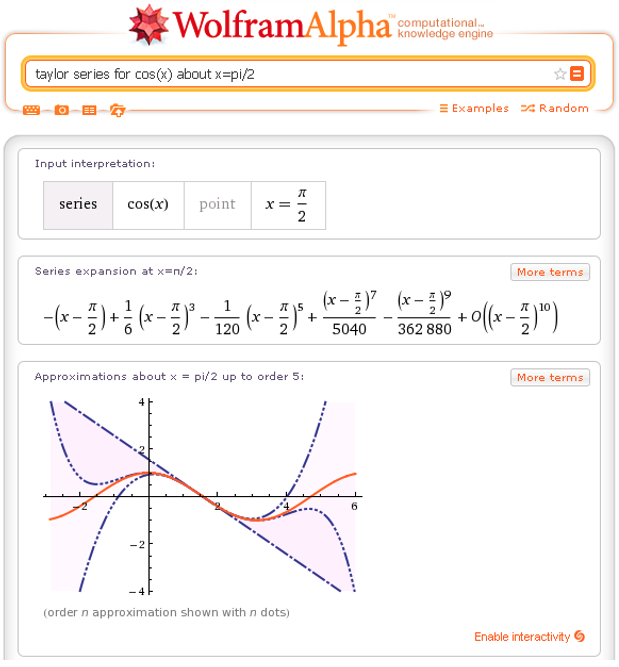
\includegraphics[width=\linewidth]{./Calculus/Images/2/Taylor_series_cos_Mathematica.png}
\end{image}%
\tcblower
\end{figureptx}%
\end{remark}
\end{sectionptx}
\end{chapterptx}
 %
%
\typeout{************************************************}
\typeout{Chapter 3 Functions of Several Variables}
\typeout{************************************************}
%
\begin{chapterptx}{Functions of Several Variables}{}{Functions of Several Variables}{}{}{x:chapter:Calculus_3}
%
%
\typeout{************************************************}
\typeout{Section 3.1 Functions of Two Variables}
\typeout{************************************************}
%
\begin{sectionptx}{Functions of Two Variables}{}{Functions of Two Variables}{}{}{x:section:functions-of-two-variables}
In Math1110 we studied "(real valued) functions of one variable", that is functions of the form,%
\begin{equation*}
f:D\rightarrow\mathbb{R}
\end{equation*}
where \(D\subseteq\mathbb{R}\) is called the domain. We used the notation \(y=f(x)\)  to denote such functions where \(x\) denotes the independent variable and \(y\) the dependent variable.%
\par
We have seen that functions of one variable are useful in practice but (of course) there are many real world relationships that are more complicated and can't be well modelled by these functions.%
\begin{example}{}{g:example:id544751}%
Suppose that we have a thin metal plate and that we are interested in the temperature \(T\) on this plate. In general the temperature will vary from point to point. If we imagine a coordinate grid on the plate then points on the plate can be identified by their coordinates \((x,y)\). Thus \(T\) will depend on two independent variables, \(x\) and \(y\). Thus we would write%
\begin{equation*}
T(x,y)
\end{equation*}
and say that \(T\) is a function of two variables. Note that functions of two variables are of the form%
\begin{equation*}
f:D\rightarrow\mathbb{R}^2
\end{equation*}
where \(D\subseteq\mathbb{R}^2\) is again the domain.%
\end{example}
Formally, we define a function of two variables as: \begin{definition}{}{g:definition:id544791}%
\terminology{A (real valued) function \(f\) of two variables} is a rule that assigns to each ordered pair of real numbers \((x,y)\) in a set \(D\) a unique (real) number denoted by \(f(x,y)\).\end{definition}
 Thus,%
\begin{equation*}
g(x,t)=\frac{\sin(t+1)}{s^2+t^2}, h(x,y)=(x-y)^2e^{-(x+y)}+6
\end{equation*}
are examples of functions of two variables.%
\par
The set \(D\) is called the \terminology{domain} of the function. Unless specified otherwise, we take \(D\) to be the largest possible set of ordered pairs for which we can calculate \(f\). The \terminology{range} of \(f\) is the associated set of values that \(f\) takes on.%
\begin{example}{}{g:example:id544815}%
Consider the function \(f(x,y)=\ln(x-y-1)\).%
\par
%
\begin{enumerate}[label=\alph*.]
\item{}Find the domain of \(f\)%
\item{}Find:%
\end{enumerate}
%
\par
%
\begin{enumerate}[label=\roman*.]
\item{}\(\displaystyle f(3,1)\)%
\item{}\(\displaystyle f(\frac{1}{2},-\sqrt{5})\)%
\item{}\(\displaystyle f(1,3)\)%
\end{enumerate}
%
\par\smallskip%
\noindent\hypertarget{g:solution:id544853}{}%
\begin{enumerate}[label=\alph*.]
\item{}Since the argument of the log function has to be positive, the domain \(D\) is the set of points in the plane satisfying%
\begin{equation*}
D=\{(x,y):y \lt x-1\}
\end{equation*}
%
\item{}%
\end{enumerate}
%
\par
%
\begin{enumerate}[label=\roman*.]
\item{}\(\displaystyle f(3,1)=\ln(3-1-1)=\ln(1)=0\)%
\item{}\(f(\frac{1}{2},-\sqrt{5})=\ln(\frac{1}{2}+\sqrt{5}-1)=\ln(\sqrt{5}-\frac{1}{2})=0.5516\) (to 4.d.p.).%
\item{}Since \((1,3)\) is not in the domain of \(f\), \(f(1,3)\) is not defined.%
\end{enumerate}
%
\end{example}
\begin{example}{}{g:example:id544882}%
Consider the function \(f(x,y)=y-xy\)%
\par
%
\begin{enumerate}[label=\alph*.]
\item{}Find the domain of \(f\)%
\item{}Find:%
\end{enumerate}
%
\par
%
\begin{enumerate}[label=\roman*.]
\item{}\(\displaystyle f(3,1)\)%
\item{}\(\displaystyle f(\frac{1}{2},-\sqrt{5})\)%
\item{}\(\displaystyle f(1,3)\)%
\end{enumerate}
%
\par\smallskip%
\noindent\hypertarget{g:solution:id544930}{}%
\begin{enumerate}[label=\alph*.]
\item{}Since we can calculate \(f\) for all values of \(x\) and \(y\) the domain of \(f\) is \(\mathbb{R}^2\)%
\item{}%
\end{enumerate}
%
\par
%
\begin{enumerate}[label=\roman*.]
\item{}\(\displaystyle f(3,1)=1-3\times 1=-2\)%
\item{}\(\displaystyle f(\frac{1}{2},-\sqrt{5})=-\sqrt{5}+\frac{1}{2}\times\sqrt{5}=-\frac{\sqrt{5}}{2}\)%
\item{}\(\displaystyle f(1,3)=3-1\times 3=0\)%
\end{enumerate}
%
\end{example}
The graph of a function of two variables is a surface in \(\mathbb{R}^3\) which passes the vertical line test. In general it is hard to draw the graph of a function of two variables by hand and so usually we get a computer to do it. The following plots have been done using the specialist mathematical software Maple but Wolfram Alpha will produce such plots too.%
\begin{example}{}{g:example:id545024}%
Produce the graph of the function \(z=f(x,y)=x^2+y^2\)%
\par\smallskip%
\noindent\hypertarget{g:solution:id545012}{}\begin{figureptx}{}{g:figure:id545004}{}%
\begin{image}{0.125}{0.75}{0.125}%
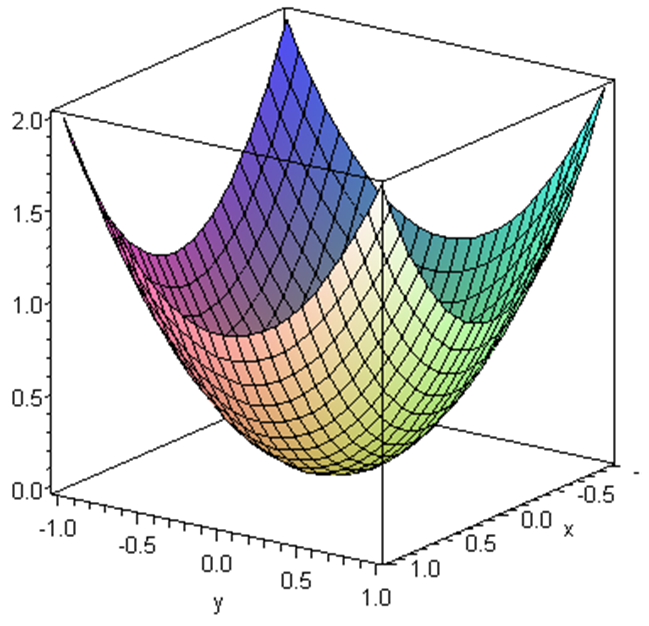
\includegraphics[width=\linewidth]{./Calculus/Images/3/1_example4.png}
\end{image}%
\tcblower
\end{figureptx}%
%
\end{example}
\begin{example}{}{g:example:id545010}%
Produce the graph of the function \(f(x,y)=x(3y-2)(5x+2)e^{-(x^2+y^2)/5}\)%
\par\smallskip%
\noindent\hypertarget{g:solution:id545019}{}\begin{figureptx}{}{g:figure:id544994}{}%
\begin{image}{0.125}{0.75}{0.125}%
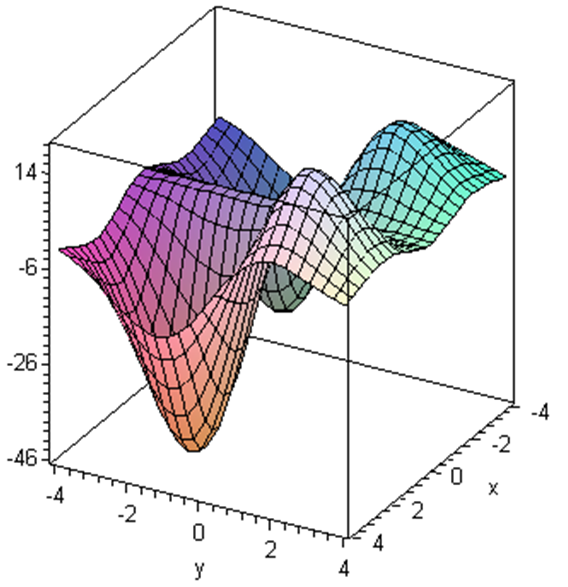
\includegraphics[width=\linewidth]{./Calculus/Images/3/1_example5.png}
\end{image}%
\tcblower
\end{figureptx}%
%
\end{example}
\begin{example}{}{g:example:id545030}%
Produce the graph of the function \(f(x,y)=\sqrt{x^2+y^2}e^{-(x^2+y^2)}\)%
\par\smallskip%
\noindent\hypertarget{g:solution:id545028}{}\begin{figureptx}{}{g:figure:id545057}{}%
\begin{image}{0}{1}{0}%
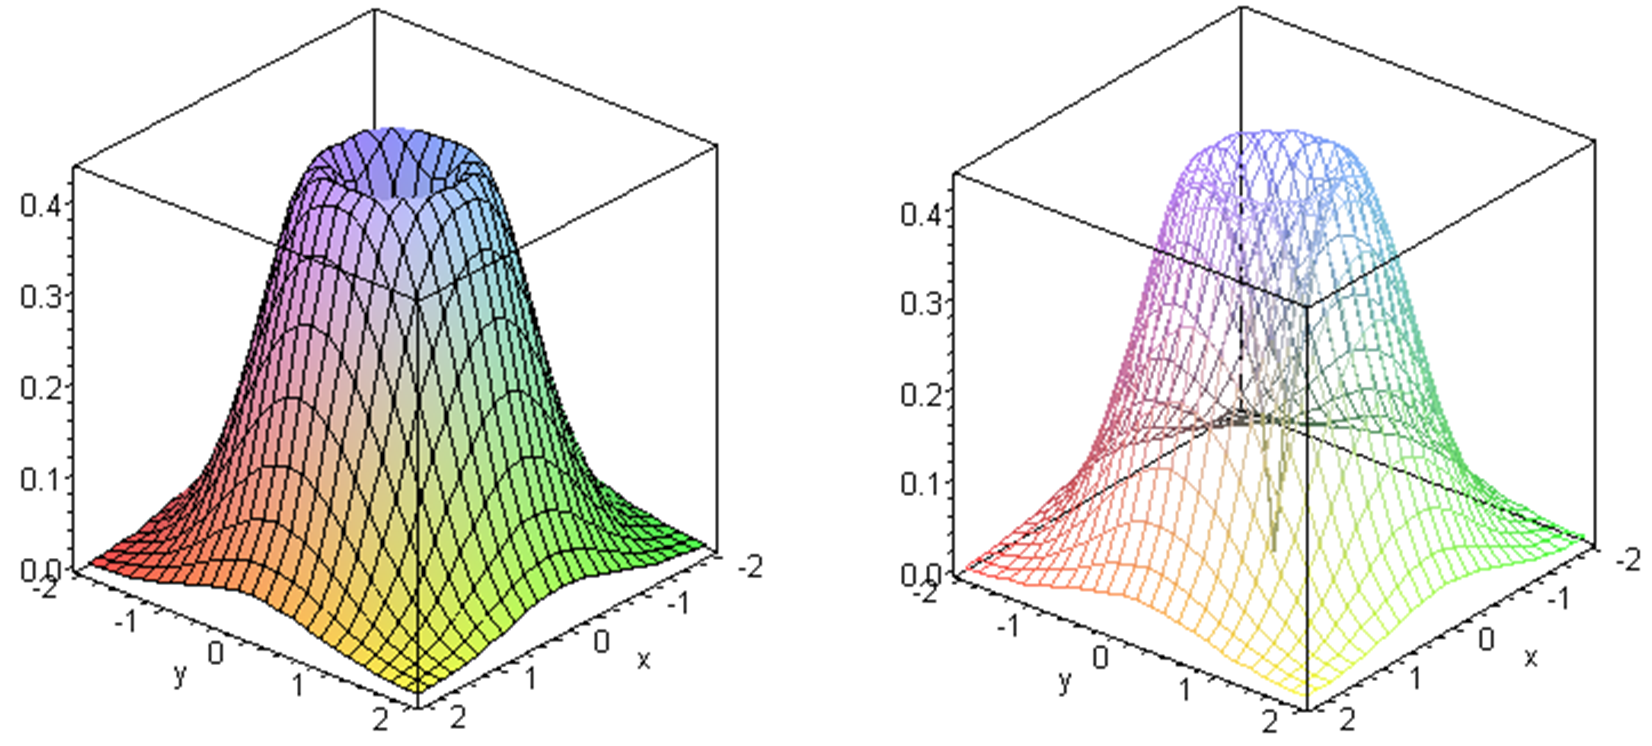
\includegraphics[width=\linewidth]{./Calculus/Images/3/1_example6.png}
\end{image}%
\tcblower
\end{figureptx}%
%
\end{example}
Not all surfaces in \(\mathbb{R}^3\) represent the graph of a function of two variables.%
\begin{example}{}{g:example:id545063}%
The surface associated the equation \(x^2+y^2+z^2=4\) is a sphere of radius \(2\) and whose centre is the origin. Clearly this surface does not pass the vertical line test. For example, when \((x,y)=(0,0)\), \(z\) could be either \(+2\) or \(-2\). \begin{figureptx}{}{g:figure:id545085}{}%
\begin{image}{0.125}{0.75}{0.125}%
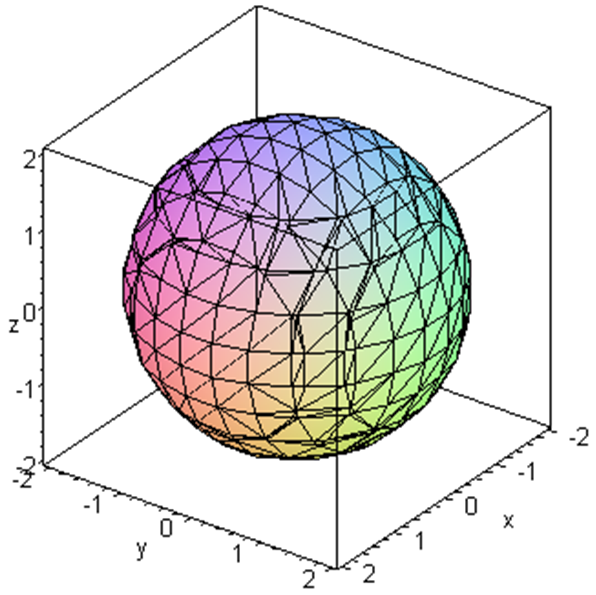
\includegraphics[width=\linewidth]{./Calculus/Images/3/1_example7.png}
\end{image}%
\tcblower
\end{figureptx}%
%
\end{example}
%
%
\typeout{************************************************}
\typeout{Exercises 3.1 Example Tasks}
\typeout{************************************************}
%
\begin{exercises-subsection-numberless}{Example Tasks}{}{Example Tasks}{}{}{g:exercises:id545068}
\begin{divisionexercise}{1}{}{}{g:exercise:id545096}%
Determine the domain of the function \(f(x,y)=\frac{\sin(y)}{xy-1}\).%
\end{divisionexercise}%
\begin{divisionexercise}{2}{}{}{g:exercise:id545091}%
Sketch the graph of the following functions.%
\par
%
\begin{enumerate}[label=\alph*.]
\item{}\(\displaystyle f(x,y)=3\)%
\item{}\(\displaystyle f(x,y)=-x-2y+2\)%
\end{enumerate}
%
\end{divisionexercise}%
\begin{divisionexercise}{3}{}{}{g:exercise:id545111}%
Sketch the surface associated with the equation \(f(x,y)=x^2+y^2-4\). Could the surface be the graph of a function of two variables?%
\end{divisionexercise}%
\end{exercises-subsection-numberless}
\end{sectionptx}
%
%
\typeout{************************************************}
\typeout{Section 3.2 Level Curves}
\typeout{************************************************}
%
\begin{sectionptx}{Level Curves}{}{Level Curves}{}{}{x:section:level-curves}
As we have seen, visualising the surface corresponding to the function \(z=f(x,y)\) can be quite difficult. One method that aids in this task is to draw level curves (sometimes known as contours). Level curves are the equivalent of contours on a topographical map. In such a map the terrain is shown by drawing curves through all points which have the same height above sea level. The numbers on the curves in the map shown below are the heights above sea level in metres. \begin{figureptx}{Sample Topographic Map (Part of the Watagan Mountains)}{g:figure:id545116}{}%
\begin{image}{0.125}{0.75}{0.125}%
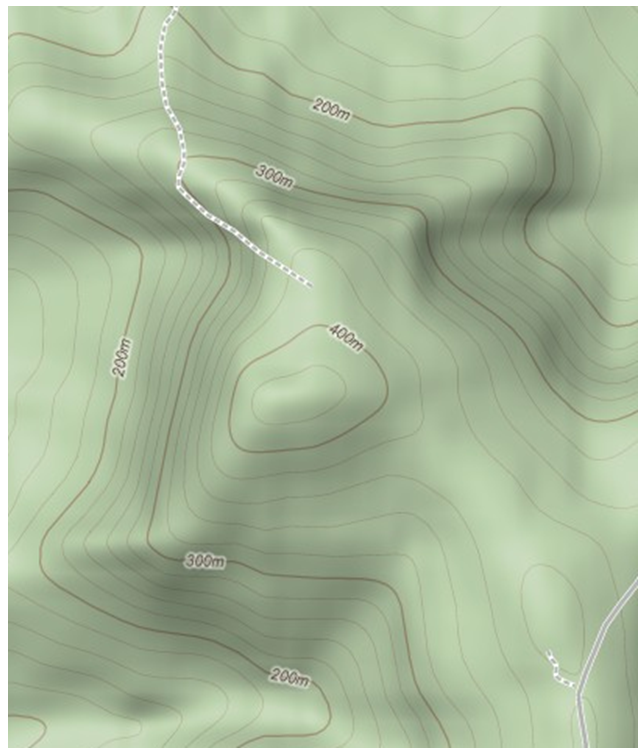
\includegraphics[width=\linewidth]{./Calculus/Images/3/2_topographicmap.png}
\end{image}%
\tcblower
\end{figureptx}%
%
\begin{definition}{}{g:definition:id545144}%
The \terminology{level curves} of a function \(z=(x,y)\) are curves in the \(xy\)-plane on which the function has the same value, i.e. on which \(z=k\), where \(k\) is some constant.\end{definition}
Note: %
\begin{enumerate}[label=\arabic*.]
\item{}Each point in the domain of the function lies on exactly one level curve.%
\item{}When a collection of level curves for a function are drawn on the same plane it is sometimes called a contour plot.%
\item{}We can also think of level curves as the intersection of the surface and the horizontal plane \(z=k\).%
\end{enumerate}
%
%
\begin{example}{}{g:example:id545219}%
Draw the level curves associated with \(k=-2,-1,0,1,2\) for the function%
\begin{equation*}
z=xy
\end{equation*}
%
\par\smallskip%
\noindent\hypertarget{g:solution:id545202}{}The level curves of a function satisfy the equation \(z=k\). So for this function the level curves are:%
\begin{equation*}
xy=k \textrm{ or }y=\frac{k}{x}
\end{equation*}
Thus the level curves are rectangular hyperbolae (except for \(k=0\)).  The level curves for \(k=-2,-1,0,1,2\) are shown in following diagram. \begin{figureptx}{}{g:figure:id545258}{}%
\begin{image}{0.125}{0.75}{0.125}%
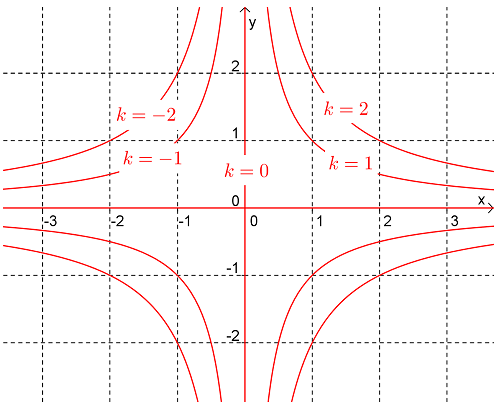
\includegraphics[width=\linewidth]{./Calculus/Images/3/2_example8.png}
\end{image}%
\tcblower
\end{figureptx}%
%
\end{example}
\begin{example}{}{g:example:id545234}%
Draw a contour plot for the function \(z=x^2+y^2\).%
\par\smallskip%
\noindent\hypertarget{g:solution:id545238}{}The contours (i.e. level curves) of a function satisfy the equation \(z=k\). So for this function the level curves are:%
\begin{equation*}
x^2+y^2=k
\end{equation*}
that is, circles centred on the origin and whose radius is \(\sqrt{k}\). \begin{figureptx}{}{g:figure:id545236}{}%
\begin{image}{0.125}{0.75}{0.125}%
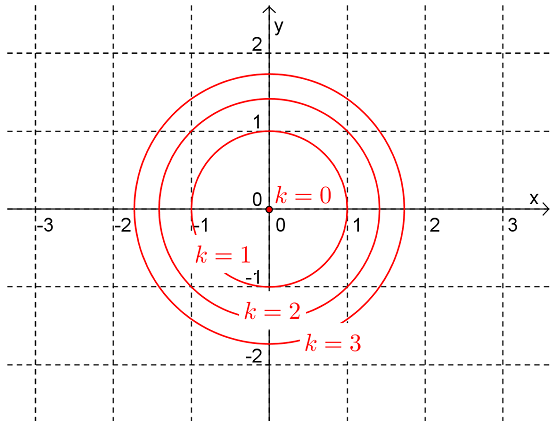
\includegraphics[width=\linewidth]{./Calculus/Images/3/2_example9.png}
\end{image}%
\tcblower
\end{figureptx}%
 Notice that there are no level curves when \(k\lt 0\). This tells us that the surface does not go below the \(xy\)-plane.%
\end{example}
%
%
\typeout{************************************************}
\typeout{Exercises 3.2 Example Tasks}
\typeout{************************************************}
%
\begin{exercises-subsection-numberless}{Example Tasks}{}{Example Tasks}{}{}{g:exercises:id545286}
\begin{divisionexercise}{1}{}{}{g:exercise:id545280}%
Draw the level curves associated with \(k=-2,-1,0,1,2\) for the function%
\begin{equation*}
z=2x-x^2+y\text{.}
\end{equation*}
%
\end{divisionexercise}%
\begin{divisionexercise}{2}{}{}{g:exercise:id545265}%
Make a rough sketch of the contour map (centred on the origin) for the function whose graph is:%
\begin{figureptx}{}{g:figure:id545282}{}%
\begin{image}{0.125}{0.75}{0.125}%
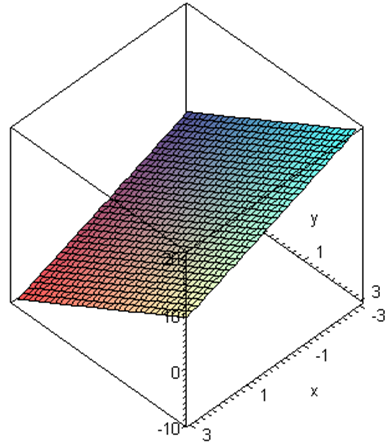
\includegraphics[width=\linewidth]{./Calculus/Images/3/2_ET2.png}
\end{image}%
\tcblower
\end{figureptx}%
\end{divisionexercise}%
\begin{divisionexercise}{3}{}{}{g:exercise:id545271}%
Make a rough sketch of the contour map (centred on the origin) for the function whose graph is:%
\begin{figureptx}{}{g:figure:id545279}{}%
\begin{image}{0.125}{0.75}{0.125}%
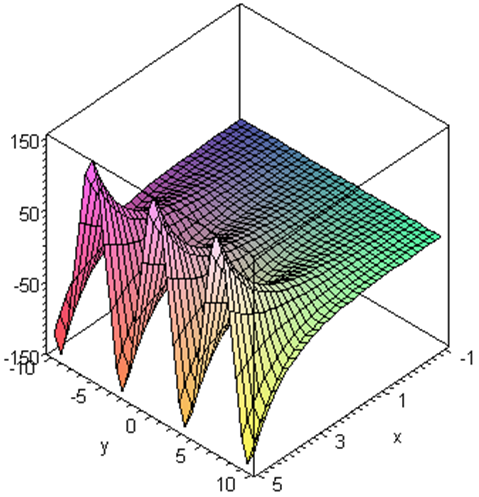
\includegraphics[width=\linewidth]{./Calculus/Images/3/2_ET3.png}
\end{image}%
\tcblower
\end{figureptx}%
\end{divisionexercise}%
\end{exercises-subsection-numberless}
\end{sectionptx}
%
%
\typeout{************************************************}
\typeout{Section 3.3 Surfaces of Revolution}
\typeout{************************************************}
%
\begin{sectionptx}{Surfaces of Revolution}{}{Surfaces of Revolution}{}{}{x:section:surfaces-of-revolution}
The surface associated with the graph of \(f(x,y)=\sqrt{x^2+y^2}e^{-(x^2+y^2)}\) (see example in section 1) is an example of a special kind of surface...a surface of revolution. \begin{definition}{}{g:definition:id545318}%
A \terminology{surface of revolution} is a surface in \(\mathbb{R}^3\) obtained by rotating a curve about an axis.\end{definition}
%
\begin{example}{}{g:example:id545306}%
Determine the equation of the surface obtained by rotating the curve in the \(xz\)-plane \(z=2-3x, x\geq 0\) about the \(z\)-axis.%
\par\smallskip%
\noindent\hypertarget{g:solution:id545373}{}\begin{figureptx}{}{g:figure:id545363}{}%
\begin{image}{0.125}{0.75}{0.125}%
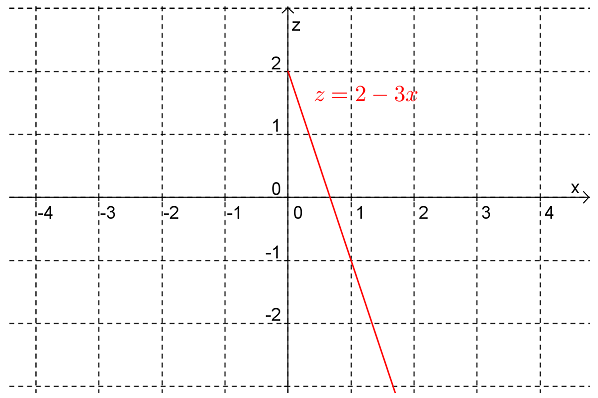
\includegraphics[width=\linewidth]{./Calculus/Images/3/3_example10.png}
\end{image}%
\tcblower
\end{figureptx}%
 Let the equation of the surface be \(z=f(x,y)\). Then the equation of the level curves of the surface will be%
\begin{equation*}
f(x,y)=k
\end{equation*}
Now, note that the cross-sections of the surface of revolution perpendicular to the \(z\)-axis (i.e. the level curves) will be circles. For example the cross section at \(z=k\) will be a circle with centre \((0,0)\) and radius \(\frac{2-k}{3}\) and hence has equation%
\begin{equation*}
x^2+y^2=\big(\frac{2-k}{3}\big)^2
\end{equation*}
On re-arranging this equation we obtain%
\begin{equation*}
k=2-3\sqrt{x^2+y^2}
\end{equation*}
Putting this into \(f(x,y)=k\) gives%
\begin{equation*}
f(x,y)=2-3\sqrt{x^2+y^2}
\end{equation*}
%
\end{example}
On repeating what we did in the above example in general gives: \begin{definition}{}{g:definition:id545409}%
The equation of a surface of revolution obtained by rotating the curve \(z=f(x), x\geq 0\) in the \(xz\)-plane about the \(z\)-axis will be%
\begin{equation*}
z=f(\sqrt{x^2+y^2})
\end{equation*}
\end{definition}
%
\begin{example}{}{g:example:id545387}%
Determine the equation of the surface obtained by rotating the curve in the \(xz\)-plane%
\begin{equation*}
z=xe^{-x^2}, x\geq 0
\end{equation*}
about the \(z\)-axis.%
\par\smallskip%
\noindent\hypertarget{g:solution:id545428}{}\begin{figureptx}{}{g:figure:id545426}{}%
\begin{image}{0.25}{0.5}{0.25}%
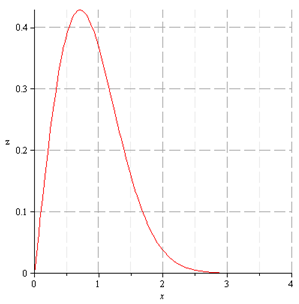
\includegraphics[width=\linewidth]{./Calculus/Images/3/3_example11.png}
\end{image}%
\tcblower
\end{figureptx}%
 The equation of the surface of revolution will be%
\begin{equation*}
z=f(\sqrt{x^2+y^2}) \textrm{ where } f(x)=xe^{-x^2}
\end{equation*}
that is,%
\begin{equation*}
z=\sqrt{x^2+y^2}e^{-\big(\sqrt{x^2+y^2}\big)^2}=\sqrt{x^2+y^2}e^{-(x^2+y^2)}
\end{equation*}
%
\end{example}
\begin{example}{}{g:example:id545432}%
Is the graph of \(f(x,y)=4-x^2-y^2\) a surface of revolution?%
\par\smallskip%
\noindent\hypertarget{g:solution:id545424}{}Since we can write the function as%
\begin{equation*}
f(x,y)=4-\big(\sqrt{x^2+y^2}\big)^2
\end{equation*}
this surface can be obtained by rotating the curve in the \(xz\)-plane%
\begin{equation*}
z=4-x^2, x\geq 0
\end{equation*}
%
\end{example}
%
%
\typeout{************************************************}
\typeout{Exercises 3.3 Example Tasks}
\typeout{************************************************}
%
\begin{exercises-subsection-numberless}{Example Tasks}{}{Example Tasks}{}{}{g:exercises:id545468}
\begin{divisionexercise}{1}{}{}{g:exercise:id545475}%
Determine the equation of the surface obtained by rotating the curve \(z=\sqrt{4-x^2}, x\geq 0\) about the \(z\)-axis. Make a sketch of the surface.%
\end{divisionexercise}%
\begin{divisionexercise}{2}{}{}{g:exercise:id545462}%
Is the graph of \(f(x,y)=xy^2-y^3\) a surface of revolution?%
\end{divisionexercise}%
\end{exercises-subsection-numberless}
\end{sectionptx}
%
%
\typeout{************************************************}
\typeout{Section 3.4 Functions of 3 (or more) Variables}
\typeout{************************************************}
%
\begin{sectionptx}{Functions of 3 (or more) Variables}{}{Functions of 3 (or more) Variables}{}{}{x:section:functions-of-3-or-more-variables}
Although we won’t do much with them in this course it is possible to define (real valued) functions in \(n\) variables where \(n\) is any natural number, that is functions of the form \(f:\mathbb{R}^n\rightarrow\mathbb{R}\).%
\begin{example}{}{g:example:id545517}%
The function \(f(x,y,z)=x^2+y^2+z^2\) is a function of the form \(f:\mathbb{R}^3\rightarrow\mathbb{R}\) .%
\end{example}
\begin{example}{}{g:example:id545513}%
The function \(f(w,x,y,z)=2wx^2+yz+\frac{w}{(x+z)}\) is a function of the form \(f:\mathbb{R}^4\rightarrow\mathbb{R}\) .%
\end{example}
Of course, for such functions geometric representations are somewhat impractical.%
\end{sectionptx}
\end{chapterptx}
 %
%
\typeout{************************************************}
\typeout{Chapter 4 Partial Differentiation}
\typeout{************************************************}
%
\begin{chapterptx}{Partial Differentiation}{}{Partial Differentiation}{}{}{x:chapter:Chap-Calculus_4}
%
%
\typeout{************************************************}
\typeout{Section 4.1 Partial Differentiation}
\typeout{************************************************}
%
\begin{sectionptx}{Partial Differentiation}{}{Partial Differentiation}{}{}{x:section:Sec-Partial_Differentiation}
Firstly, let’s recall some of the important things that we know about the derivative of the function of one variable, \(f(x)\).%
\par
%
\begin{enumerate}[label=\roman*]
\item{}At any given point \(x_0\), \(f'(x_0)\) gives the slope of the tangent to the graph of the function at that point. \begin{figureptx}{}{x:figure:Fig-Slope_of_tangent}{}%
\begin{image}{0.075}{0.85}{0.075}%
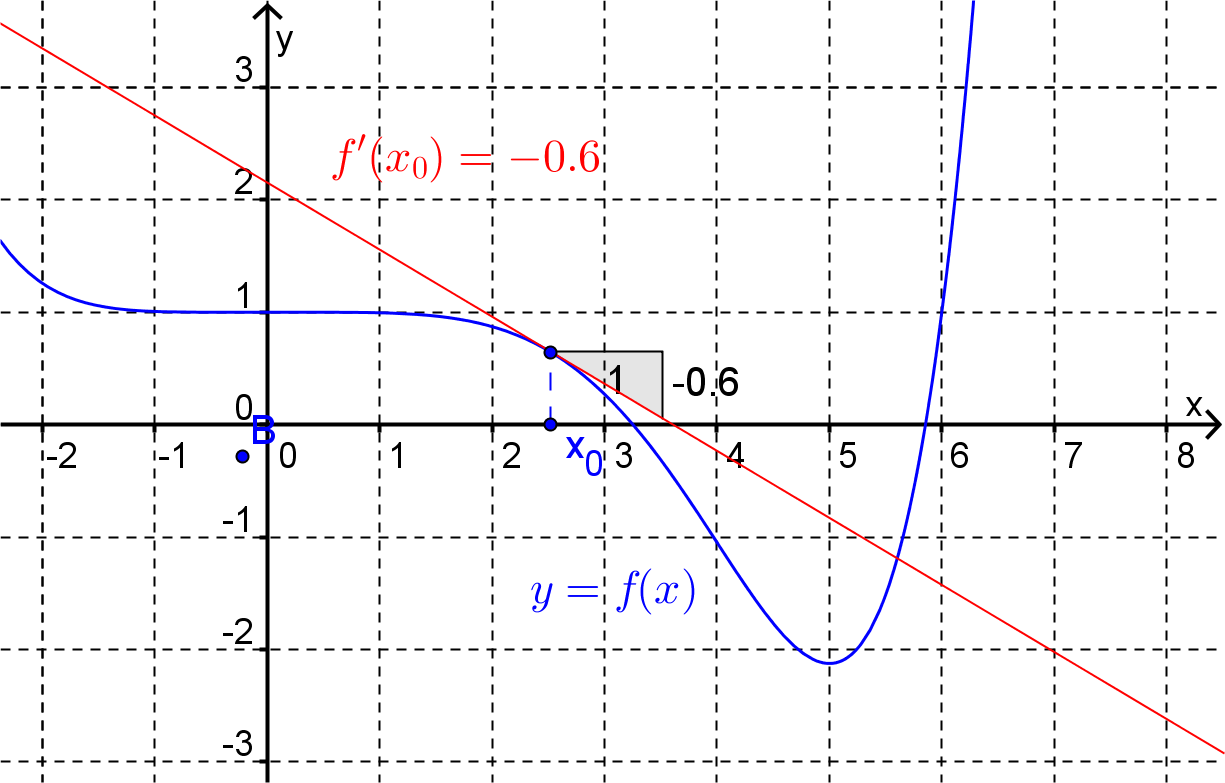
\includegraphics[width=\linewidth]{./Calculus/Images/4/Slope_of_tangent.png}
\end{image}%
\tcblower
\end{figureptx}%
%
\item{}At any given point \(x_0\), \(f'(x_0)\) gives the instantaneous rate of change of the function at that point.%
\item{}The derivative \(f'(x)\) is itself a function of one variable, when it exists.%
\end{enumerate}
%
\par
For a function of two variables,  , the rate at which the function is changing at any point as we vary the independent variables depends upon the direction in which we vary those variables.%
\begin{example}{}{x:example:Ex-Direction_and_rate_of_change}%
Consider the function \(f(x,y) = x^2-y^2\). The graph of this function is shown below. At \((x,y)=(0,0)\), \(f=0\). As we can see by looking at the graph, as we move away from the origin along the positive \(x\)-axis the value of \(f\) is increasing, i.e. the rate of change of the function will be positive. However, if we move away from the origin along the positive \(y\)-axis the value of \(f\) is decreasing, i.e. the rate of change of the function will be negative.%
\begin{figureptx}{}{x:figure:Fig-Example_1_Contour_Plot}{}%
\begin{image}{0.15}{0.7}{0.15}%
\includegraphics[width=\linewidth]{./Calculus/Images/4/Ex1_Contour_Plot_Fig_1.png}
\end{image}%
\tcblower
\end{figureptx}%
\end{example}
As a first step to analyzing more formally how a function of two variables can change with respect to its independent variables we will first consider the cases where we vary only one variable at a time.%
\begin{example}{}{x:example:Ex-Direction_and_instantaneous_rate_of_change}%
Consider the function \(f(x,y) = 5 - \dfrac{x^2+y^2}{2}\) at the point \((2,1)\).%
\par
Firstly, let’s look at the instantaneous rate of change of \(f\) in the direction of the positive \(x\)-axis, As shown in the diagram below, if we hold \(y\) constant at and vary \(x\) we are actually moving along the curve%
\begin{equation*}
z=\frac{9}{2}-\frac{1}{2}x^2\text{.}
\end{equation*}
%
\begin{figureptx}{}{x:figure:Fig-Example_2_x_axis}{}%
\begin{image}{0.15}{0.7}{0.15}%
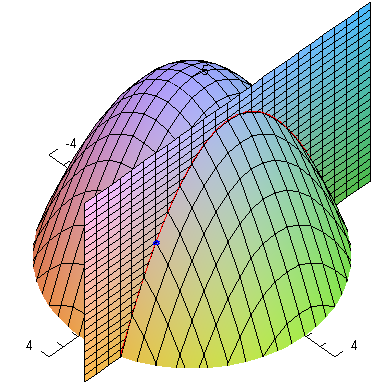
\includegraphics[width=\linewidth]{./Calculus/Images/4/Ex2_x_axis_rate_of_change.png}
\end{image}%
\tcblower
\end{figureptx}%
Along this curve \(\dfrac{dz}{dx}=-x\) and at \(x=2\) we have \(\dfrac{dz}{dx}=-2\). Thus, the instantaneous rate of change of \(f\) in the direction of the positive \(x\)-axis at the point \((2,1)\) is \(-2\).%
\par
Now consider the instantaneous rate of change of \(f\) in the direction of the positive \(y\)-axis. As shown in the diagram below, if we hold \(x\) constant at \(x=2\) and vary \(y\) we are actually moving along the curve%
\begin{equation*}
z=3-\frac{1}{2}y^2\text{.}
\end{equation*}
%
\par
Along this curve \(\dfrac{dz}{dy}=-y\) and at \(y=1\) we have \(\dfrac{dz}{dy}=-1\). Thus, the instantaneous rate of change of \(f\) in the direction of the positive \(y\)-axis at the point \((2,1)\) is \(-1\).%
\begin{figureptx}{}{x:figure:Fig-Example_2_y_axis}{}%
\begin{image}{0.15}{0.7}{0.15}%
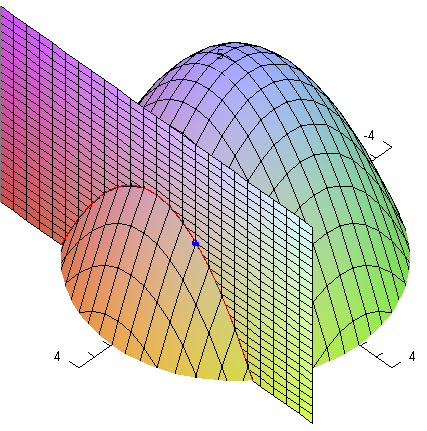
\includegraphics[width=\linewidth]{./Calculus/Images/4/Ex2_y_axis_rate_of_change.png}
\end{image}%
\tcblower
\end{figureptx}%
\end{example}
The above example provided an illustration of calculating what are called partial derivatives. Formally partial derivatives are defined as follows.%
\begin{definition}{Partial Derivative.}{g:definition:id545830}%
Consider the function of two variables, \(f(x,y)\)%
\par
The \terminology{partial derivative of \(f\) with respect to \(x\)} at the point \((x_0,y_0)\) is given by the limit (if it exists)%
\begin{equation*}
\frac{\partial f}{\partial x} (x_0,y_0) = \lim_{h \to 0} \left[ \frac{f(x_0+h,y_0)-f(x_0,y_0)}{h} \right]\text{.}
\end{equation*}
%
\par
The \terminology{partial derivative of \(f\) with respect to \(y\)} at the point \((x_0,y_0)\) is given by the limit (if it exists)%
\begin{equation*}
\frac{\partial f}{\partial y} (x_0,y_0) = \lim_{h \to 0} \left[ \frac{f(x_0,y_0+h)-f(x_0,y_0)}{h} \right]\text{.}
\end{equation*}
%
\end{definition}
\begin{example}{}{x:example:Ex-Calculating_partial_derivatives_at_particular_point}%
Using the definition, calculate the partial derivatives of \(f(x,y) = 5 - \dfrac{x^2+y^2}{2}\) at the point \((2,1)\).%
\par\smallskip%
\noindent\textbf{\blocktitlefont Answer}.\hypertarget{g:answer:id545867}{}\quad{}\(\dfrac{\partial f}{\partial x}(2,1) = -2\) and \(\dfrac{\partial f}{\partial y}(2,1) = -1\)%
\par\smallskip%
\noindent\textbf{\blocktitlefont Solution}.\hypertarget{g:solution:id545879}{}\quad{}Firstly, calculate the partial derivative of \(f\) with respect to \(x\) at \((2,1)\).%
\par
%
\begin{align*}
\frac{\partial f}{\partial x}(2,1) \amp = \lim_{h \to 0} \left[ \frac{f(2+h,1)-f(2,1)}{h} \right]\\
\amp = \lim_{h \to 0} \left[\frac{1}{h} \left( \left( 5 - \frac{(2+h)^2 + 1^2}{2} \right) - \left( 5 - \frac{2^2+1^2}{2} \right) \right) \right]\\
\amp = \lim_{h \to 0} \left[\frac{1}{h} \left( -\frac{1}{2}(4+4h+h^2+1) +\frac{1}{2}(4+1) \right) \right]\\
\amp = \lim_{h \to 0} \left[ \frac{1}{h} \left(-2h-\frac{1}{2}h^2 \right) \right]\\
\amp = -2
\end{align*}
%
\par
Next, calculate the partial derivative of \(f\) with respect to \(y\) at \((2,1)\).%
\par
%
\begin{align*}
\frac{\partial f}{\partial x}(2,1) \amp = \lim_{h \to 0} \left[ \frac{f(2,1+h)-f(2,1)}{h} \right]\\
\amp = \lim_{h \to 0} \left[\frac{1}{h} \left( \left( 5 - \frac{2^2 + (1+h)^2}{2} \right) - \left( 5 - \frac{2^2+1^2}{2} \right) \right) \right]\\
\amp = \lim_{h \to 0} \left[\frac{1}{h} \left( -\frac{1}{2}(4+1+2h+h^2) +\frac{1}{2}(4+1) \right) \right]\\
\amp = \lim_{h \to 0} \left[ \frac{1}{h} \left(-h-\frac{1}{2}h^2 \right) \right]\\
\amp = -1
\end{align*}
%
\end{example}
If we calculate the partial derivatives of a function at the general point \((x,y)\) (as opposed to some specific point \((x_0,y_0)\)) we will obtain (instead of two specific values) two new functions of two variables.%
\begin{example}{}{x:example:Ex-Calculating_partial_derivatives_at_general_point}%
Using the definition, calculate the partial derivatives of \(f(x,y) = xy-1\).%
\par\smallskip%
\noindent\textbf{\blocktitlefont Answer}.\hypertarget{g:answer:id545950}{}\quad{}\(\dfrac{\partial f}{\partial x}(x,y) = y\) and \(\dfrac{\partial f}{\partial y}(x,y) = x\)%
\par\smallskip%
\noindent\textbf{\blocktitlefont Solution}.\hypertarget{g:solution:id545963}{}\quad{}Calculating the partial derivative with respect to \(x\):%
\par
%
\begin{align*}
\frac{\partial f}{\partial x}(x,y) \amp = \lim_{h \to 0} \left[ \frac{f(x+h,y)-f(x,y)}{h} \right]\\
\amp = \lim_{h \to 0} \left[ \frac{\left( (x+h)y-1 \right)-(xy-1)}{h} \right]\\
\amp = \lim_{h \to 0} \left[ \frac{hy}{h} \right]\\
\amp = y
\end{align*}
%
\par
Now, calculating the partial derivative with respect to \(y\):%
\par
%
\begin{align*}
\frac{\partial f}{\partial y}(x,y) \amp = \lim_{h \to 0} \left[ \frac{f(x,y+h)-f(x,y)}{h} \right]\\
\amp = \lim_{h \to 0} \left[ \frac{\left( x(y+h)-1 \right)-(xy-1)}{h} \right]\\
\amp = \lim_{h \to 0} \left[ \frac{hx}{h} \right]\\
\amp = x
\end{align*}
%
\end{example}
As can be seen in the above example, to calculate the partial derivative of \(f\) with respect to \(x\) at the general point \((x,y)\) all we have to do is treat \(y\) as a constant and differentiate \(f(x,y)\) with respect to \(x\) (using all of the familiar rules of differentiation for functions of one variable). Similarly, to calculate the partial derivative of \(f\) with respect to \(y\) at the general point \((x,y)\) treat \(x\) as a constant and differentiate \(f(x,y)\) with respect to \(y\).%
\begin{example}{}{x:example:Ex-Calculating_partial_derivatives_at_particular_point_shorter}%
Find the partial derivatives of the function \(f(x,y) = 5 - \frac{x^2+y^2}{2}\) at the point \((2,1)\) using the above method.%
\par\smallskip%
\noindent\textbf{\blocktitlefont Answer}.\hypertarget{g:answer:id546074}{}\quad{}\(\dfrac{\partial f}{\partial x}(2,1) = -2\) and \(\dfrac{\partial f}{\partial y}(2,1) = -1\)%
\par\smallskip%
\noindent\textbf{\blocktitlefont Solution}.\hypertarget{g:solution:id546076}{}\quad{}This function can be written as:%
\par
%
\begin{equation*}
f(x,y) = 5 - \frac{1}{2}x^2 - \frac{1}{2}y^2.
\end{equation*}
%
\par
Now, thinking of \(y\) as a constant (so that \(\frac{1}{2}y^2\) is also constant) and treating the function as a function of \(x\) only,%
\par
%
\begin{equation*}
\dfrac{\partial f}{\partial x}(x,y) = 0 - 2 \times \frac{1}{2}x - 0 = -x.
\end{equation*}
%
\par
Thus,%
\par
%
\begin{equation*}
\dfrac{\partial f}{\partial x}(2,1) = -2.
\end{equation*}
%
\par
Next, think of \(x\) as a constant (so that \(\frac{1}{2}x^2\) is also constant) and treating the function as a function of \(y\) only,%
\par
%
\begin{equation*}
\dfrac{\partial f}{\partial y}(x,y) = 0-0-2\times \frac{1}{2} y = -y.
\end{equation*}
%
\par
Thus,%
\par
%
\begin{equation*}
\dfrac{\partial f}{\partial y}(2,1) = -1.
\end{equation*}
%
\end{example}
A shorter notation for the partial derivative of \(f\) with respect to \(x\) is \(f_x\). Similarly the partial derivative with respect to \(y\) is written as \(f_y\).%
\begin{example}{}{x:example:Ex-shorthand_computation_example-1}%
Find \(f_x\) and \(f_y\) when \(f(x,y) = x^2y\).%
\par\smallskip%
\noindent\textbf{\blocktitlefont Solution}.\hypertarget{g:solution:id546143}{}\quad{}To find \(f_x (x,y)\), think of \(y\) as a constant. Thus,%
\begin{equation*}
f_x(x,y) = 2xy\text{.}
\end{equation*}
%
\par
To find \(f_y (x,y)\), think of \(x\) as a constant. So,%
\begin{equation*}
f_y(x,y) = x^2\text{.}
\end{equation*}
%
\end{example}
\begin{example}{}{x:example:Ex-shorthand_computation_example_arcsin}%
Find \(f_x\) and \(f_y\) when \(f(x,y) = \sin^{-1}\left(\frac{x}{y}\right) - 5x^2\).%
\par\smallskip%
\noindent\textbf{\blocktitlefont Solution}.\hypertarget{g:solution:id546206}{}\quad{}To find \(f_x (x,y)\), think of \(y\) as a constant. Thus, using the chain rule:%
\begin{align*}
f_x(x,y) \amp = \frac{1}{\sqrt{1 - \left(\dfrac{x}{y}\right)^2 }} \cdot \frac{1}{y} - 10x\\
\amp = \frac{1}{\sqrt{y^2 - x^2}} - 10x\text{.}
\end{align*}
%
\par
To find \(f_y (x,y)\), think of \(x\) as a constant. Again, using the chain rule:%
\begin{align*}
f_y(x,y) \amp = \frac{1}{\sqrt{1 - \left(\dfrac{x}{y}\right)^2 }} \cdot \left( \frac{-x}{y^2} \right) - 0\\
\amp = \frac{-x}{y\sqrt{y^2-x^2}}.
\end{align*}
%
\end{example}
\begin{example}{}{x:example:Ex-shorthand_computation_example-3_variables_implicit}%
The equation \(xz + y^2z^3 = 2\) can be thought of as implicitly defining \(z\) as a function of \(x\) and \(y\). Find \(z_x\) and \(z_y\).%
\par\smallskip%
\noindent\textbf{\blocktitlefont Solution}.\hypertarget{g:solution:id546290}{}\quad{}To find \(z_x\) differentiate both sides of the defining equation with respect to \(x\), remembering that \(z\) is some unknown function of \(x\). Also, remember to treat \(y\) as a constant. Then, using the product rule and the chain rule,%
\par
%
\begin{align*}
\frac{\partial}{\partial x} \left(xz + y^2z^3 \right) \amp = \frac{\partial}{\partial x} (2)\\
xz_x + z + 3y^2 z^2 z_x \amp = 0\\
z_x (x+3y^2 z^2) \amp = -z\\
z_x \amp = \frac{-z}{x+3y^2 z^2}
\end{align*}
%
\par
Similarly, differentiating both sides of the defining equation with respect to \(y\),%
\par
%
\begin{align*}
\frac{\partial}{\partial y} \left(xz + y^2z^3 \right) \amp = \frac{\partial}{\partial y} (2)\\
xz_y + 2yz^3 + 3y^2 z^2 z_y \amp = 0\\
z_y (x+3y^2 z^2) \amp = -2yz^3\\
z_y \amp = \frac{-2yz^3}{x+3y^2 z^2}
\end{align*}
%
\end{example}
Partial derivatives can be found for functions of more than two variables.%
\begin{example}{}{x:example:Ex-shorthand_computation_example_3_variables}%
Find the partial derivatives for the function of three variables%
\begin{equation*}
f(x,y,z) = (2x+3y-z^2)e^{xz}\text{.}
\end{equation*}
%
\par\smallskip%
\noindent\textbf{\blocktitlefont Solution}.\hypertarget{g:solution:id546335}{}\quad{}Write the function as%
\begin{equation*}
f(x,y,z) = 2xe^{xz} + 3ye^{xz} - z^2 e^{xz}\text{.}
\end{equation*}
%
\par
To find \(f_x\) treat \(y\) and \(z\) as constants and think of \(f\) as a function of \(x\) only. Thus,%
\par
%
\begin{align*}
f_x(x,y,z) \amp = (2xz e^{xz} + 2e^{xz} ) + 3yze^{xz} - z^3 e^{xz}\\
\amp = e^{xz} (2xz + 3yz - z^3 + 2)
\end{align*}
%
\par
To find \(f_y\) treat \(x\) and \(z\) as constants and think of \(f\) as a function of \(y\) only. Thus,%
\par
%
\begin{align*}
f_y(x,y,z) \amp = 0 + 3e^{xz} - 0\\
\amp = 3e^{xz}
\end{align*}
%
\par
Finally, to find \(f_z\) treat \(x\) and \(y\) as constants and think of \(f\) as a function of \(z\) only. Thus,%
\par
%
\begin{align*}
f_z(x,y,z) \amp = 2x^2 e^{xz} + 3xye^{xz} - (xz^2e^{xz} + 2ze^{xz} )\\
\amp = e^{xz} (2x^2 + 3xy - xz^2 - 2z)
\end{align*}
%
\end{example}
%
%
\typeout{************************************************}
\typeout{Exercises 4.1 Example Tasks}
\typeout{************************************************}
%
\begin{exercises-subsection-numberless}{Example Tasks}{}{Example Tasks}{}{}{g:exercises:id546447}
\begin{divisionexercise}{1}{}{}{g:exercise:id546424}%
Find both partial derivatives of the function \(f(x,y)=4-xy-y^2\) at the point \((3,2)\).%
\end{divisionexercise}%
\begin{divisionexercise}{2}{}{}{g:exercise:id546429}%
Find \(\dfrac{\partial f}{\partial x}\) and \(\dfrac{\partial f}{\partial y}\) when \(f(x,y) = \ln(x^2-4xy^3)\).%
\end{divisionexercise}%
\begin{divisionexercise}{3}{}{}{g:exercise:id546455}%
If \(L(x,y) = \dfrac{e^{xy}}{(1-x)(1-y)}\), find \(L_x(2,3)\).%
\end{divisionexercise}%
\begin{divisionexercise}{4}{}{}{g:exercise:id546456}%
Find \(f_x(x,y)\) and \(f_y(x,y)\) when \(f(x,y) = x^y\).%
\end{divisionexercise}%
\begin{divisionexercise}{5}{}{}{g:exercise:id546489}%
In the following contour plot the contours are for evenly spaced values of \(k\) from \(-2\) at the point \(X\) to \(2\) at the point \(Y\). Find the sign of \(f_x(x,y)\) and \(f_y(x,y)\) at the points \(A\), \(B\) and \(C\) given the following contour plot for the function \(f(x,y)\). Explain your thinking.%
\begin{figureptx}{}{x:figure:Fig-Contour_plot}{}%
\begin{image}{0.15}{0.7}{0.15}%
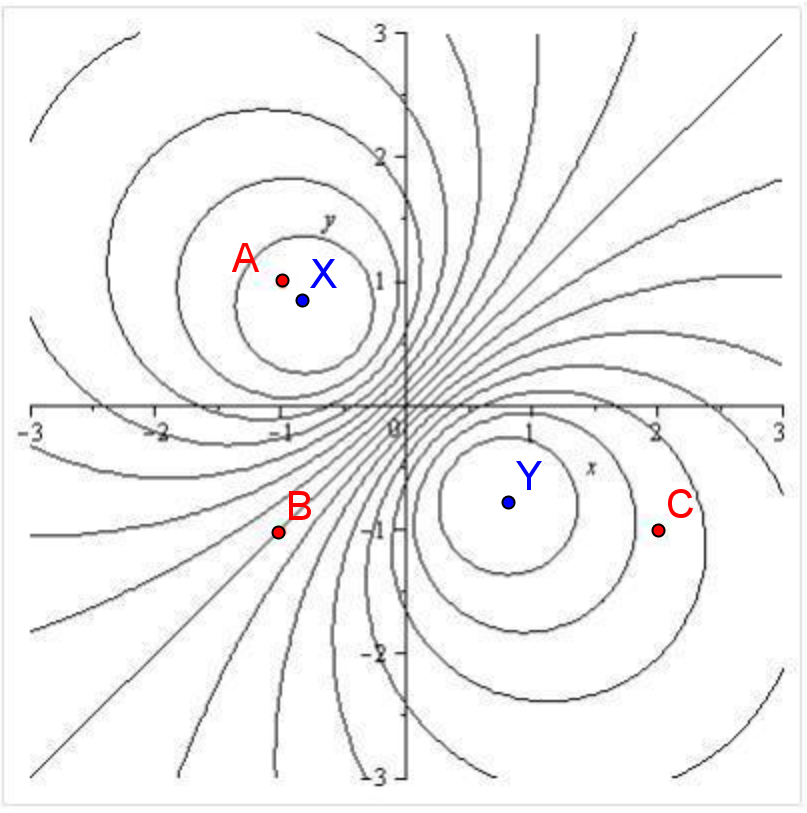
\includegraphics[width=\linewidth]{./Calculus/Images/4/Contour_plot.png}
\end{image}%
\tcblower
\end{figureptx}%
\end{divisionexercise}%
\end{exercises-subsection-numberless}
\end{sectionptx}
%
%
\typeout{************************************************}
\typeout{Section 4.2 Higher Partial Derivatives}
\typeout{************************************************}
%
\begin{sectionptx}{Higher Partial Derivatives}{}{Higher Partial Derivatives}{}{}{x:section:Sec-Higher_Partial_Derivatives}
The partial derivatives of the function \(z=f(x,y)\) are themselves functions of two variables. Thus they can be differentiated further, giving the second partial derivatives, the third partial derivatives etc. Common notations for the second partial derivatives include:%
\par
%
\begin{alignat*}{2}
\dfrac{\partial}{\partial x} \left( \dfrac{\partial f}{\partial x} \right) \amp = \dfrac{\partial^2 f}{\partial x^2} \amp = (f_x)_x \amp = f_{xx}\\
\dfrac{\partial}{\partial y} \left( \dfrac{\partial f}{\partial x} \right) \amp = \dfrac{\partial^2 f}{\partial y \partial x} \amp = (f_x)_y \amp = f_{xy}\\
\dfrac{\partial}{\partial x} \left( \dfrac{\partial f}{\partial y} \right) \amp = \dfrac{\partial^2 f}{\partial x \partial y} \amp = (f_y)_x \amp = f_{yx}\\
\dfrac{\partial}{\partial y} \left( \dfrac{\partial f}{\partial y} \right) \amp = \dfrac{\partial^2 f}{\partial y^2} \amp = (f_y)_y \amp = f_{yy}
\end{alignat*}
%
\begin{example}{}{x:example:Ex-second_partial_derivatives}%
Find the second partial derivatives for the function%
\begin{equation*}
f(x,y) = \sin(x) \cos(y)\text{.}
\end{equation*}
%
\par\smallskip%
\noindent\textbf{\blocktitlefont Solution}.\hypertarget{g:solution:id546567}{}\quad{}Begin by finding the first partial derivatives. Here%
\begin{align*}
\amp f_x(x,y) = \cos(x)\cos(y) \amp \text{and} \amp \amp f_y(x,y) = - \sin(x) \sin(y)\text{.}
\end{align*}
%
\par
Now differentiate \(f_x(x,y)\) firstly with respect to \(x\) to find \(f_{xx}(x,y)\) and then with respect to \(y\) to find \(f_{xy}(x,y)\). Thus,%
\begin{align*}
f_{xx}(x,y) \amp = -\sin(x) \cos(y), \, \, \text{and}\\
f_{xy}(x,y) \amp = -\cos(x) \sin(y).
\end{align*}
%
\par
Next differentiate \(f_y(x,y)\) with respect to \(x\) to find \(f_{yx}(x,y)\) and then with respect to \(y\) to find \(f_{yy}(x,y)\). Thus,%
\begin{align*}
f_{yx}(x,y) \amp = -\cos(x) \sin(y), \, \, \text{and}\\
f_{yy}(x,y) \amp = -\sin(x) \cos(y).
\end{align*}
%
\par
Notice that for this function \(f_{xy}(x,y) = f_{yx}(x,y)\).%
\end{example}
\begin{example}{}{x:example:Ex-third_partial_derivatives}%
Calculate \(g_{xxy}\), \(g_{xyx}\) and \(g_{yxx}\) when \(g(x)=xy^2 + \dfrac{y}{x^2}\).%
\par\smallskip%
\noindent\textbf{\blocktitlefont Solution}.\hypertarget{g:solution:id546675}{}\quad{}Begin by writing the function in the form%
\begin{equation*}
g(x,y) = xy^2 + yx^{-2}\text{.}
\end{equation*}
%
\par
Then the first partial derivatives are%
\begin{align*}
\amp g_x = y^2 - 2yx^{-3} \amp \text{and} \amp \amp g_y = 2xy+x^{-2}
\end{align*}
and hence the second partial derivatives are%
\begin{equation*}
g_{xx}=6yx^{-4}, \;  g_{xy} = 2y-2x^{-3}, \;  g_{yx} = 2y-2x^{-3}, \; g_{yy} = 2x\text{.}
\end{equation*}
%
\par
Differentiating \(g_{xx}\) with respect to \(y\), \(g_{xy}\) with respect to \(x\) and \(g_{yx}\) with respect to \(x\) gives%
\begin{equation*}
g_{xxy} = 6x^{-4}, \; g_{xyx} = 6x^{-4}, \; g_{yxx} = 6x^{-4}\text{.}
\end{equation*}
%
\end{example}
The above instances have provided examples of the following general result.%
\begin{theorem}{Clairaut's Theorem.}{}{g:theorem:id546706}%
If for the function \(f(x,y)\) both \(f_{xy}\) and \(f_{yx}\) are continuous on some domain \(D\), then on that domain%
\begin{equation*}
f_{xy}(x,y) = f_{yx}(x,y)\text{.}
\end{equation*}
%
\end{theorem}
Clairaut’s Theorem can be extended to higher partial derivatives and to functions of more than two variables.%
\begin{example}{}{x:example:Ex-first_and_second_partials_of_3_variable_function}%
Calculate all first and second order partial derivatives for the function%
\begin{equation*}
g(x,y,z) = \dfrac{x^2 + 3y^2}{1+2z}\text{.}
\end{equation*}
%
\par\smallskip%
\noindent\textbf{\blocktitlefont Solution}.\hypertarget{g:solution:id546738}{}\quad{}Even though \(g\) is a function of \(3\) variables, Clairaut's Theorem still holds. Thus there will be only 6 distinct second partial derivatives, i.e. \(g_{xx}\), \(g_{xy}\), \(g_{xz}\), \(g_{yy}\), \(g_{yz}\), \(g_{zz}\).%
\par
Now%
\begin{equation*}
g_x = \dfrac{2x}{1+2z}, \,\, g_y = \dfrac{6y}{1+2z}, \,\, g_z = \dfrac{-2(x^2+3y^2)}{(1+2z)^2}
\end{equation*}
and so%
\begin{equation*}
g_{xx} = \dfrac{2}{1+2z}, \,\, g_{xy} = 0, \,\, g_{xz} = \dfrac{-4x}{(1+2z)^2},
\end{equation*}
%
\begin{equation*}
g_{yz} = \dfrac{-12y}{(1+2z)^2}, \,\, g_{yy} = \dfrac{6}{1+2z}, \,\, g_{zz} = \dfrac{8(x^2+3y^2)}{(1+2z)^3}.
\end{equation*}
%
\end{example}
%
%
\typeout{************************************************}
\typeout{Exercises 4.2 Example Tasks}
\typeout{************************************************}
%
\begin{exercises-subsection-numberless}{Example Tasks}{}{Example Tasks}{}{}{g:exercises:id546813}
\begin{divisionexercise}{1}{}{}{g:exercise:id546796}%
Find the second partial derivatives for the function \(z=xye^y\).%
\end{divisionexercise}%
\begin{divisionexercise}{2}{}{}{g:exercise:id546800}%
Calculate \(g_{xx},\,\) \(g_{xy}\) and \(g_{xyy}\) for \(g(x,y) = \dfrac{y}{1+x^2}\).%
\end{divisionexercise}%
\begin{divisionexercise}{3}{}{}{g:exercise:id548208}%
Let \(u(x,t) = e^{-t} \sin \left(\frac{x}{c}\right)\) where \(c\) is a constant and \(c>0\). Determine if \(u\) satisfies%
\begin{equation*}
\dfrac{\partial u}{\partial t} = c^2 \dfrac{\partial^2 u}{\partial x^2}
\end{equation*}
%
\end{divisionexercise}%
\end{exercises-subsection-numberless}
\begin{remark}{A little remark.}{g:remark:id548258}%
Computer algebra systems can find partial derivatives. For example, here are some examples of a queries to Wolfram Alpha that will work.%
\begin{figureptx}{}{x:figure:Fig-WA_1}{}%
\begin{image}{0.05}{0.9}{0.05}%
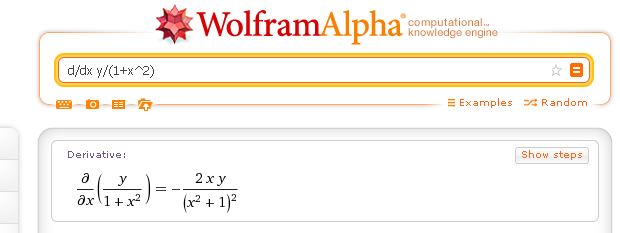
\includegraphics[width=\linewidth]{./Calculus/Images/4/WA_1.png}
\end{image}%
\tcblower
\end{figureptx}%
\begin{figureptx}{}{x:figure:Fig-WA_2}{}%
\begin{image}{0.05}{0.9}{0.05}%
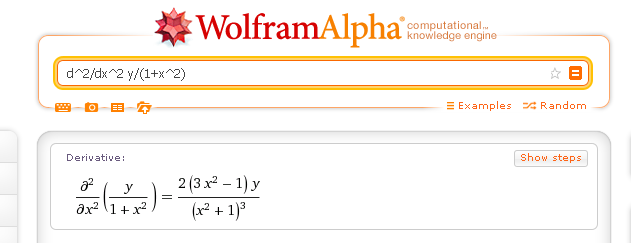
\includegraphics[width=\linewidth]{./Calculus/Images/4/WA_2.png}
\end{image}%
\tcblower
\end{figureptx}%
\begin{figureptx}{}{x:figure:Fig-WA_3}{}%
\begin{image}{0.05}{0.9}{0.05}%
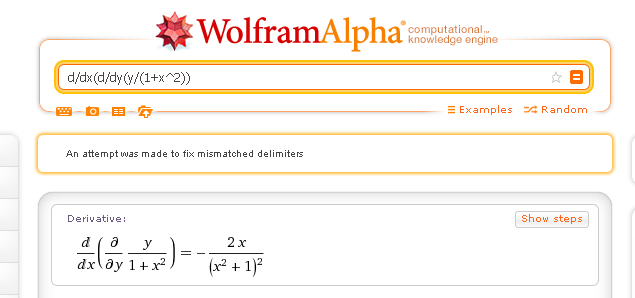
\includegraphics[width=\linewidth]{./Calculus/Images/4/WA_3.png}
\end{image}%
\tcblower
\end{figureptx}%
\end{remark}
\end{sectionptx}
\end{chapterptx}
 %
%
\typeout{************************************************}
\typeout{Chapter 5 Linear Approximations}
\typeout{************************************************}
%
\begin{chapterptx}{Linear Approximations}{}{Linear Approximations}{}{}{x:chapter:Chap-Calculus_5}
\begin{introduction}{}%
In Math1110 we looked at the idea of ``the linearization of a function of one variable''. The idea was that near the point \(x=x_0\) we could approximate the function \(f(x)\) using the line tangent to the function at \(x=x_0\). We called this tangent the linearization of the function at \(x=x_0\) and used it to derive the ``linear approximation formula'',%
\begin{equation*}
\Delta y \simeq f'(x_0) \Delta x\text{.}
\end{equation*}
These ideas can also be applied to functions of two variables.%
\end{introduction}%
%
%
\typeout{************************************************}
\typeout{Section 5.1 Tangent Planes}
\typeout{************************************************}
%
\begin{sectionptx}{Tangent Planes}{}{Tangent Planes}{}{}{x:section:Sec-Tangent_Planes}
Recall  that  the  graph  associated  with  the  function \(z=f(x,y)\) is  a  surface  in \(\mathbb{R}^3\) (that passes the vertical line test). Wherever this surface does not have any discontinuities or cusp-like points it will have a tangent plane. Like the tangent line to the graph of a function of one variable,  the  tangent  plane  to  the  function \(z=f(x,y)\) at  the  point \((x_0,y_0)\) is  the  plane  that ``just touches'' the surface at the point \((x_0,y_0,z_0)\).%
\begin{example}{}{x:example:Ex-Tangent_Plane}%
For  the  function \(f(x,y) = 5-\dfrac{x^2+y^2}{2}\) the  graph  below  shows  the  graph of the function and it’s tangent plane at the point \((x,y) = (2,1)\).%
\begin{figureptx}{}{x:figure:Fig-Example_1_Tangent_Plane}{}%
\begin{image}{0.15}{0.7}{0.15}%
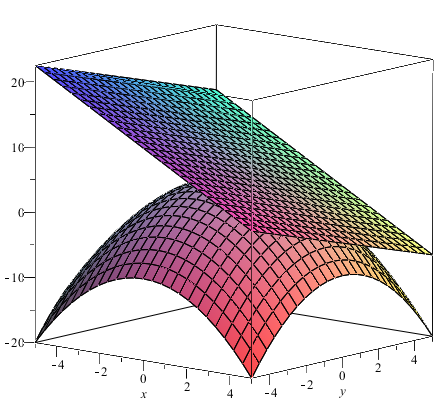
\includegraphics[width=\linewidth]{./Calculus/Images/5/Ex1_Tangent_Plane.png}
\end{image}%
\tcblower
\end{figureptx}%
\end{example}
To find the equation of the plane tangent to the function \(z=f(x,y)\) at the point \((x_0,y_0,z_0)\), firstly recall that the equation of a plane in Cartesian form is given by%
\begin{equation*}
ax+by+cz = k, \quad a,b,c,k \in \mathbb{R},
\end{equation*}
or in normal form, as illustrated in \hyperref[x:figure:Fig-Tangent_Plane_Vector_Form_Figure]{Figure~{\xreffont\ref{x:figure:Fig-Tangent_Plane_Vector_Form_Figure}}}, by%
\begin{equation}
\bm{n} \cdot (\bm{r}-\bm{r}_0) = 0\label{x:men:Eqn-Tangent_Plane_Vector_Form}
\end{equation}
where \(\bm{n} = \langle a,b,c \rangle\) is a normal vector to the plane, \(\bm{r}_0\) is the position vector of a point on the plane and \(\bm{r} = \langle x,y,z \rangle\).%
\begin{figureptx}{}{x:figure:Fig-Tangent_Plane_Vector_Form_Figure}{}%
\begin{image}{0.15}{0.7}{0.15}%
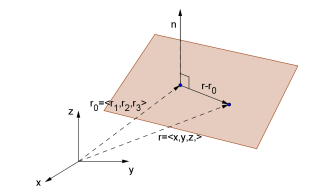
\includegraphics[width=\linewidth]{./Calculus/Images/5/Tangent_Plane_Vector_Form.png}
\end{image}%
\tcblower
\end{figureptx}%
\begin{example}{}{x:example:Ex-Equation_of_Tangent_Plane}%
Find the equation of the tangent plane to the function \(f(x,y) = 5-\dfrac{x^2+y^2}{2}\) at \((x,y) = (2,1)\).%
\par\smallskip%
\noindent\textbf{\blocktitlefont Answer}.\hypertarget{g:answer:id548430}{}\quad{}\(2x+y+z=\dfrac{15}{2}\)%
\par\smallskip%
\noindent\textbf{\blocktitlefont Solution}.\hypertarget{g:solution:id548460}{}\quad{}Now, we know that the partial derivative \(f_x(2,1)\) gives the slope of the tangent at \(x=2\), to the curve of intersection of the surface associated with \(f\) and the plane \(y=1\).%
\begin{figureptx}{}{x:figure:Fig-Example_2_Tangent_Planes}{}%
\begin{image}{0.15}{0.7}{0.15}%
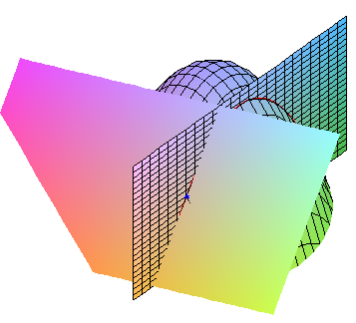
\includegraphics[width=\linewidth]{./Calculus/Images/5/Ex2_Tangent_Planes.png}
\end{image}%
\tcblower
\end{figureptx}%
Since this tangent line lies in the plane tangent to \(f\) at \((x,y) = (2,1)\) the vector%
\begin{equation*}
\langle 1,0,f_x(2,1) \rangle
\end{equation*}
will be a vector that is parallel to the tangent plane, (or lies in the tangent plane if we place it’s tail at the point \((2,1,\frac{5}{2})\)). Similarly, the vector%
\begin{equation*}
\langle 0,1,f_y(2,1) \rangle
\end{equation*}
will be another vector parallel to the tangent plane. Since these two non-parallel vectors are parallel to the tangent plane, their vector product will give a vector normal to the tangent plane, i.e.%
\begin{align*}
\bm{n} \amp = \langle 1,0,f_x(2,1) \rangle \times \langle 0,1,f_y(2,1) \rangle\\
\amp = \langle -f_x(2,1), -f_y(2,1), 1 \rangle\\
\amp = \langle 2,1,1 \rangle
\end{align*}
Thus, using equation \hyperref[x:men:Eqn-Tangent_Plane_Vector_Form]{({\xreffont\ref{x:men:Eqn-Tangent_Plane_Vector_Form}})}, the equation of the plane tangent to \(f(x,y) = 5 - \dfrac{x^2+y^2}{2}\) at \((x,y) = (2,1)\) is%
\begin{equation*}
\langle 2,1,1 \rangle \cdot \left( \langle x,y,z \rangle - \langle 2,1,\frac{5}{2} \rangle \right) = 0
\end{equation*}
which simplifies to%
\begin{equation*}
2x+y+z=\frac{15}{2}\text{.}
\end{equation*}
%
\end{example}
In general, to find the equation of the plane tangent to the function \(f(x,y)\) at the point \((x_0,y_0)\), note that the vectors%
\begin{equation*}
\langle 1, 0, f_x(x_0,y_0) \rangle \: \text{and} \: \langle 0,1,f_y(x_0,y_0) \rangle
\end{equation*}
lie in the tangent plane and hence a normal to the plane is%
\begin{align*}
\bm{n} \amp = \langle 1, 0 f_x(x_0,y_0) \rangle \times \langle0,1,f_y(x_0,y_0) \rangle\\
\amp = \langle -f_x(x_0,y_0), -f_y(x_0,y_0),1 \rangle\text{.}
\end{align*}
Since the point \((x_0,y_0,z_0)\) lies on the plane, using equation \hyperref[x:men:Eqn-Tangent_Plane_Vector_Form]{({\xreffont\ref{x:men:Eqn-Tangent_Plane_Vector_Form}})}, the equation of the tangent plane is%
\begin{equation*}
\langle  -f_x(x_0,y_0), -f_y(x_0,y_0),1 \rangle \cdot \bigg( \langle x,y,z \rangle - \langle x_0, y_0, z_0 \rangle \bigg) = 0.
\end{equation*}
On expanding and rearranging this we get the following result.%
\begin{theorem}{}{}{x:theorem:Thm-Equation-of-tangent-plane}%
The equation of the plane tangent to the function \(f(x,y)\) at the point \((x_0,y_0,z_0)\) is%
\begin{equation*}
z = z_0 + f_x(x_0,y_0) (x-x_0) + f_y(x_0,y_0) (y-y_0)\text{,}
\end{equation*}
where \(z_0 = f(x_0,y_0)\).%
\end{theorem}
\begin{example}{}{x:example:Ex-Equation_of_Tangent_Plane_2}%
Find the equation of the plane tangent to \(z = x^2+2y^2\) at the point \((x,y)=(1,2)\).%
\begin{figureptx}{}{x:figure:Fig-Example_3_Tangent_Plane}{}%
\begin{image}{0.15}{0.7}{0.15}%
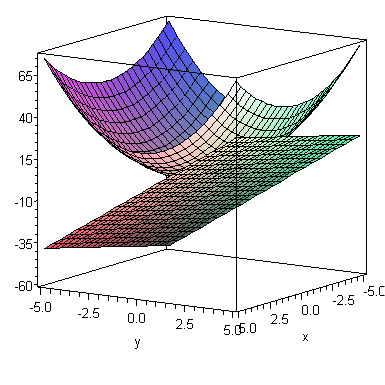
\includegraphics[width=\linewidth]{./Calculus/Images/5/Ex3_Tangent_Plane.png}
\end{image}%
\tcblower
\end{figureptx}%
\par\smallskip%
\noindent\textbf{\blocktitlefont Answer}.\hypertarget{g:answer:id548590}{}\quad{}\(2x+8y-z-9=0\)%
\par\smallskip%
\noindent\textbf{\blocktitlefont Solution}.\hypertarget{g:solution:id548584}{}\quad{}Firstly, note that when \((x,y)=(1,2)\), \(z=9\). Now%
\begin{equation*}
z_x = 2x \: \text{ and so } \: z_x(1,2) = 2
\end{equation*}
and%
\begin{equation*}
z_y = 4y \: \text{ and so } \: z_y(1,2) = 8\text{.}
\end{equation*}
Thus the equation of the tangent plane is%
\begin{equation*}
z = 9+2(x-1)+8(y-2)
\end{equation*}
which simplifies to%
\begin{equation*}
2x+8y-z-9=0\text{.}
\end{equation*}
%
\end{example}
\begin{example}{}{x:example:Ex-Equation_of_Normal_Line}%
Find the equation of the line normal to the graph of the function \(z=x^2+2y^2\) at the point \((x,y) = (1,2)\).%
\par\smallskip%
\noindent\textbf{\blocktitlefont Answer}.\hypertarget{g:answer:id548623}{}\quad{}\(\bm{r} = \langle 1, 2, 9 \rangle + t \langle -2, -8, 1 \rangle\)%
\par\smallskip%
\noindent\textbf{\blocktitlefont Solution}.\hypertarget{g:solution:id548625}{}\quad{}Recall that the vector equation of a line in \(\mathbb{R}^3\) is%
\begin{equation*}
\bm{r} = \bm{r}_0 + t \bm{d}, \: t \in \mathbb{R}
\end{equation*}
where \(\bm{r} = \langle x, y, z \rangle\) is the position vector of a general point, \(\bm{r}_0\) is the position vector of a point that lies on the line and \(d\) is a direction vector for the line (i.e. a vector that is parallel to the line).%
\par
We know that a vector normal to the surface \(z=f(x,y)\) at the point \((x_0,y_0,z_0)\) is given by%
\begin{equation*}
\bm{n} = \langle -f_x(x_0,y_0), -f_y(x_0,y_0),1 \rangle\text{.}
\end{equation*}
%
\par
For the function \(z=x^2+2y^2\), \(z_x=2x\) and \(z_y=4y\). Thus a direction vector for the line normal to \(z=x^2+2y^2\) at the point \((x,y)=(1,2)\) will be%
\begin{equation*}
\bm{d} = \langle -2, -8, 1 \rangle\text{.}
\end{equation*}
Since the normal line passes through the point \((1,2,9)\) its equation is%
\begin{equation*}
\bm{r} = \langle 1, 2, 9 \rangle + t \langle -2, -8, 1 \rangle\text{.}
\end{equation*}
%
\end{example}
%
%
\typeout{************************************************}
\typeout{Exercises 5.1 Example Tasks}
\typeout{************************************************}
%
\begin{exercises-subsection-numberless}{Example Tasks}{}{Example Tasks}{}{}{g:exercises:id548709}
\begin{divisionexercise}{1}{}{}{g:exercise:id548706}%
Find the equation of the tangent plane to \(z=x^2-5xy+2y^2\) at the point \((x,y)=(1,2)\).%
\end{divisionexercise}%
\begin{divisionexercise}{2}{}{}{g:exercise:id548724}%
Find the equation of the tangent plane and normal line to \(z = \sqrt{x+y} \sin (xy)\) at the point \((x,y)=(0,1)\).%
\end{divisionexercise}%
\begin{divisionexercise}{3}{}{}{g:exercise:id548754}%
Show that every line that is normal to the sphere \(x^2+y^2+z^2 = 1\) passes through the origin.%
\end{divisionexercise}%
\end{exercises-subsection-numberless}
\end{sectionptx}
%
%
\typeout{************************************************}
\typeout{Section 5.2 Linear Approximations}
\typeout{************************************************}
%
\begin{sectionptx}{Linear Approximations}{}{Linear Approximations}{}{}{x:section:Sec-Linear_Approximations}
In Section \hyperref[x:section:Sec-Tangent_Planes]{Section~{\xreffont\ref{x:section:Sec-Tangent_Planes}}} we found that the equation of the tangent plane to the function \(f(x,y)\) at the point \((x_0,y_0,f(x_0,y_0))\), which is a linear equation.%
\begin{definition}{}{g:definition:id548740}%
We call the function%
\begin{equation*}
L(x,y) = f(x_0,y_0) + f_x(x_0,y_0)(x-x_0) + f_y(x_0,y_0)(y-y_0)
\end{equation*}
the linearisation of \(f\) at the point \((x_0,y_0)\).%
\end{definition}
\begin{example}{}{x:example:Ex-Linearisation}%
Find the linearisation of \(z=\sin(x)\cos(y)\) at the point \((x,y) = \left(\dfrac{\pi}{4},\dfrac{\pi}{4} \right)\).%
\par\smallskip%
\noindent\textbf{\blocktitlefont Answer}.\hypertarget{g:answer:id548784}{}\quad{}\(L(x,y) = \dfrac{1}{2} + \dfrac{1}{2} \left( x - \dfrac{\pi}{4} \right) - \dfrac{1}{2} \left(y - \dfrac{\pi}{4} \right)\)%
\par\smallskip%
\noindent\textbf{\blocktitlefont Solution}.\hypertarget{g:solution:id548787}{}\quad{}Begin by calculating the partial derivatives of \(z\),%
\begin{equation*}
z_x = \cos(x)\cos(y) \: \text{ and } \: z_y = -\sin(x)\sin(y)\text{.}
\end{equation*}
Thus%
\begin{alignat*}{2}
z \left(\dfrac{\pi}{4},\dfrac{\pi}{4} \right) \amp = \, \, \, \, \sin \left(\dfrac{\pi}{4} \right) \cos \left(\dfrac{\pi}{4} \right) \amp = \dfrac{1}{2}\\
z_x \left(\dfrac{\pi}{4},\dfrac{\pi}{4} \right) \amp = \, \, \, \, \cos \left(\dfrac{\pi}{4} \right) \cos \left(\dfrac{\pi}{4} \right) \amp = \dfrac{1}{2}\\
z_y \left(\dfrac{\pi}{4},\dfrac{\pi}{4} \right) \amp = -\sin \left(\dfrac{\pi}{4} \right) \sin \left(\dfrac{\pi}{4} \right) \amp = \dfrac{1}{2}\text{.}
\end{alignat*}
and so the linearisation is%
\begin{equation*}
L(x,y) = \dfrac{1}{2} + \dfrac{1}{2} \left( x - \dfrac{\pi}{4} \right) - \dfrac{1}{2} \left(y - \dfrac{\pi}{4} \right)\text{.}
\end{equation*}
%
\end{example}
When we use the linearisation of \(f\) at the point \((x_0,y_0)\) to approximate the function near the point \((x_0,y_0)\) we call this the \emph{linear (or tangent plane) approximation} of \(f\) at the point \((x_0,y_0)\). Notice that if we let the independent variables change by the amounts \(\Delta x\) and \(\Delta y\) then the linearisation will change from \(L(x_0,y_0)\) to \(L(x_0+\Delta x, y_0 + \Delta y)\). Thus we can approximate the change in the function value \(z=f(x,y)\) by%
\begin{equation*}
\Delta z \simeq L(x_0 + \Delta x, y_0 + \Delta y) - L(x_0,y_0).
\end{equation*}
On using the linearisation formula given above, we end up with the following result.%
\begin{definition}{The Linear Approximation Formula.}{g:definition:id548871}%
The  linear  approximation  to  the  change, \(\Delta z\),  in  the  function \(z = f(x,y)\) when  the independent variables change from \((x_0,y_0)\) to \((x_0+\Delta x, y_0 + \Delta y)\) is%
\begin{equation*}
\Delta z \simeq f_x (x_0, y_0) \Delta x + f_y (x_0, y_0) \Delta y\text{.}
\end{equation*}
%
\end{definition}
This result is sometimes called the ``small change'' formula for functions of two variables.%
\begin{example}{}{x:example:Ex-Linear-Estimation}%
For the function \(f(x,y) = 3x^4+2y^4\), \(f(1,2) = 35\). Use a linear approximation to estimate \(f(1.01,2.03)\).%
\par\smallskip%
\noindent\textbf{\blocktitlefont Answer}.\hypertarget{g:answer:id548937}{}\quad{}\(f(1.01,2.03) \simeq 37.04\)%
\par\smallskip%
\noindent\textbf{\blocktitlefont Solution}.\hypertarget{g:solution:id548935}{}\quad{}Via a linear approximation%
\begin{equation*}
f(1.01,2.03) \simeq f(1,2) + \Delta f\text{.}
\end{equation*}
Here%
\begin{equation*}
f_x = 12x^3 \: \text{ and } \: f_y = 8y^3
\end{equation*}
and so%
\begin{equation*}
f_x(1,2) = 12 \: \text{ and } \: f_y(1,2) = 64\text{.}
\end{equation*}
%
\par
Thus, with \(\Delta x = 0.01\) and \(\Delta y = 0.03\), via the linear approximation formula%
\begin{equation*}
\Delta f = 12 \times 0.01 + 64 \times 0.03 = 2.04
\end{equation*}
and hence%
\begin{equation*}
f(1.01,2.03) \simeq 35 + 2.04 = 37.04
\end{equation*}
%
\end{example}
\begin{example}{}{x:example:Ex-Find_Density_of_Steel_Ball}%
A steel ball has a mass, \(m\), of 6300 \(\pm\) \SI{50}{\gram} and has volume, \(V\), 800 \(\pm\) \SI{10}{\centi\meter\tothe{3}}. Find the density of the ball, including an estimate of the error.%
\par\smallskip%
\noindent\textbf{\blocktitlefont Answer}.\hypertarget{g:answer:id548979}{}\quad{}\(\rho = \) 7.875 \(\pm \) \SI{0.1609375}{\gram\per\centi\meter\tothe{3}}%
\par\smallskip%
\noindent\textbf{\blocktitlefont Solution}.\hypertarget{g:solution:id549033}{}\quad{}The density, \(\rho\), is given by%
\begin{equation*}
\rho = \dfrac{m}{V}\text{.}
\end{equation*}
Thus%
\begin{equation*}
\rho = \dfrac{6300}{800} = 7.875 \: g/cm^3.
\end{equation*}
%
\par
Using a linear approximation to estimate the error%
\begin{equation*}
\Delta \rho \simeq \dfrac{\partial \rho}{\partial m} \Delta m + \dfrac{\partial \rho}{\partial V} \Delta V\text{.}
\end{equation*}
Now%
\begin{equation*}
\dfrac{\partial \rho}{\partial m} = \dfrac{1}{V} \: \text{ and } \: \dfrac{\partial \rho}{\partial V} = -\dfrac{m}{V^2}
\end{equation*}
and so at \(m=6300\), \(V=800\) and with \(\Delta m = 50\) and \(\Delta V = -10\) (to get the maximum value of \(\Delta \rho\))%
\begin{equation*}
\Delta \rho \simeq \frac{1}{800} \times 50 + \frac{6300}{800^2} \times 10 = 0.1609375\text{.}
\end{equation*}
Thus%
\begin{equation*}
\rho = 7.875 \pm 0.1609375 \: g/cm^3\text{.}
\end{equation*}
%
\end{example}
\begin{example}{}{x:example:Ex-Linear-Estimation_Implicit}%
Use a linear approximation to estimate the value of \(z\) at \((x,y) = (1.1,-0.02)\) for surface \(z = f(x,y)\) defined implicitly by \(z-yz^3 = x+2\).%
\par\smallskip%
\noindent\textbf{\blocktitlefont Answer}.\hypertarget{g:answer:id549115}{}\quad{}\(z(1.1,-0.02) \simeq 2.56\)%
\par\smallskip%
\noindent\textbf{\blocktitlefont Solution}.\hypertarget{g:solution:id549086}{}\quad{}Firstly  notice  that  when \(x=1\) and \(y=0\), \(z=3\). Thus \(z(1,0)=3\). Now, via a linear approximation%
\begin{equation*}
z(1.1,-0.02) \simeq z(1,0) + \Delta z
\end{equation*}
where%
\begin{equation*}
\Delta z \simeq z_x(1,0) \Delta x + z_y(1,0) \Delta y\text{,}
\end{equation*}
and \(\Delta x = 0.1\), \(\Delta y = -0.02\). To find the partial derivatives we need to use implicit differentiation. Differentiating with respect to \(x\):%
\begin{align*}
\dfrac{\partial}{\partial x} (z - yz^3) \amp = \dfrac{\partial}{\partial x} (x+2)\\
z_x - 3y z^2 z_x \amp = 1\\
z_x \amp = \dfrac{1}{1-3yz^2}\text{.}
\end{align*}
%
\par
Thus%
\begin{equation*}
z_x(1,0) = \dfrac{1}{1-3 \times 0 \times 3^2} = 1\text{.}
\end{equation*}
%
\par
Differentiating with respect to y:%
\begin{align*}
\dfrac{\partial}{\partial y} (z - yz^3) \amp = \dfrac{\partial}{\partial y} (x+2)\\
z_y - (3y z^2 z_y + z^3) \amp = 0\\
z_y \amp = \dfrac{z^3}{1-3yz^2}\text{.}
\end{align*}
%
\par
Thus%
\begin{equation*}
z_y(1,0) = \dfrac{3^3}{1-3 \times 0 \times 3^2} = 27\text{.}
\end{equation*}
Putting this together gives%
\begin{equation*}
\Delta z \simeq 1 \times 0.1 + 27 \times (-0.02) = -0.44
\end{equation*}
and hence%
\begin{equation*}
z(1.1,-0.02) \simeq 3-0.44 = 2.56.
\end{equation*}
%
\end{example}
%
%
\typeout{************************************************}
\typeout{Exercises 5.2 Example Tasks}
\typeout{************************************************}
%
\begin{exercises-subsection-numberless}{Example Tasks}{}{Example Tasks}{}{}{g:exercises:id549187}
\begin{divisionexercise}{1}{}{}{g:exercise:id549182}%
Use a linear approximation to find the value of \(z(2.96,-0.95)\) when%
\begin{equation*}
z=x^2-xy+3y^2\text{.}
\end{equation*}
%
\end{divisionexercise}%
\begin{divisionexercise}{2}{}{}{g:exercise:id549162}%
Use a linear approximation to estimate the value of \(\sqrt{(2.01)^2-0.98}\).%
\end{divisionexercise}%
\begin{divisionexercise}{3}{}{}{g:exercise:id549214}%
A right angled triangle \(ABC\) with right angle at \(B\) is measured with \(AB = \) 10 \(\pm\) \SI{0.02}{\centi\meter} and \(BC = \) 3.4 \(\pm\) \SI{0.02}{\centi\meter}. What is the angle at \(A\), including the error?%
\end{divisionexercise}%
\begin{divisionexercise}{4}{}{}{g:exercise:id549255}%
In the figure below a rectangle initially with sides \(x\) and \(y\) has been made larger so that the sides are now \(x + \Delta x\) and \(y + \Delta y\). \begin{figureptx}{}{x:figure:Fig-Task_4_Figure}{}%
\begin{image}{0.2}{0.6}{0.2}%
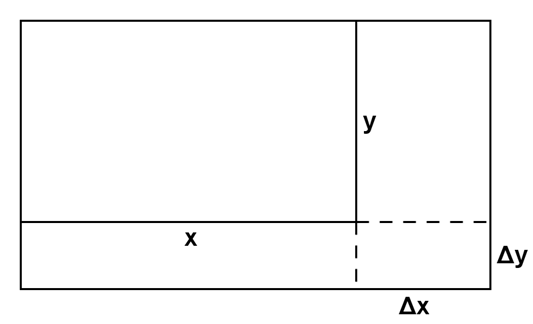
\includegraphics[width=\linewidth]{./Calculus/Images/5/Task_4_Figure.png}
\end{image}%
\tcblower
\end{figureptx}%
 Shade on the diagram the regions that represent:%
\begin{enumerate}[label=\alph*]
\item{}The increase in area.%
\item{}The linear approximation to the increase in area. Explain your answer.%
\end{enumerate}
%
\end{divisionexercise}%
\end{exercises-subsection-numberless}
\end{sectionptx}
%
%
\typeout{************************************************}
\typeout{Section 5.3 Quadratic Approximations}
\typeout{************************************************}
%
\begin{sectionptx}{Quadratic Approximations}{}{Quadratic Approximations}{}{}{x:section:Quadratic-Approximations}
We have seen previously that for functions of one variable the idea of the linearisation of the function could be extended by considering the Taylor polynomial for the function.%
\begin{example}{}{x:example:Ex-Exp_Function_Maclaurin_polynomial_of_degree_2}%
For the function \(f(x) = e^x\) the Maclaurin polynomial of degree \(n\) is%
\begin{equation*}
\sum_{k=0}^{n} \dfrac{x^k}{k!} = 1+x+\dfrac{x^2}{2!}+\ldots+\dfrac{x^n}{n!}\text{.}
\end{equation*}
%
\par
We saw that the linearisation of \(e^x\) at \(x=0\) was the Maclaurin polynomial of degree 1, i.e.%
\begin{equation*}
T_1 (x) = 1+x\text{.}
\end{equation*}
%
\par
The Maclaurin polynomial of degree 2, i.e.%
\begin{equation*}
T_2 (x) = 1 + x + \dfrac{x^2}{2}
\end{equation*}
gives a quadratic approximation to \(e^x\) about \(x=0\) and so on.%
\end{example}
For functions of one variable we derived the Taylor series by trying to find a power series in \((x-a)\) that matched the function and all its derivatives at \(x=a\). For functions of two variables we can use a similar idea to derive the Taylor series about the point \((x,y)=(a,b)\). This series will be a power series in \((x-a)\) and \((y-b)\) that matches the function and its partial derivatives at the point \((x,y)=(a,b)\). The formula for the Taylor series of two variables is quite lengthy to write and so we will not reproduce it here. However, as with functions of one variable truncations of this series are called Taylor polynomials and the Taylor polynomial of degree 1 is the linearisation of the function. Similarly, the Taylor polynomial of degree 2 will give us a quadratic approximation to the function.%
\begin{definition}{Taylor Polynomial of Degree 2.}{g:definition:id549378}%
The Taylor Polynomial of degree 2 for the function of two variables \(f(x,y)\) about the point \((x,y) = (a,b)\) is%
\begin{align*}
T_2(x,y) = \amp f(a,b) + f_x(a,b)(x-a) + f_y(a,b)(y-b)\\
\amp + \dfrac{f_{xx}(a,b)}{2!} (x-a)^2 + f_{xy}(a,b)(x-a)(y-b) + \dfrac{f_{yy}(a,b)}{2!}(y-b)^2
\end{align*}
\end{definition}
The question of how good an approximation this polynomial is goes beyond what we will cover in this course but if \(f(x,y)\) has continuous partial derivatives and if \((x,y)\) is ``sufficiently close to'' \((a,b)\) then the approximation should be useful.%
\begin{example}{}{x:example:Ex-Find_quadratic_approx}%
Find the quadratic approximation to the function \(f(x,y) = x^2y\) about the point \((x,y) = (1,2)\).%
\par\smallskip%
\noindent\textbf{\blocktitlefont Solution}.\hypertarget{g:solution:id549417}{}\quad{}First calculate the partial derivatives:%
\begin{equation*}
f_x = 2xy, \: \: f_y = x^2, \: \: f_{xx} = 2y, \: \: f_{xy} = 2x, \: \: f_{yy} = 0.
\end{equation*}
%
\par
Now evaluate these at \((x,y) = (1,2)\)%
\begin{equation*}
f_x(1,2) = 4, \: \: f_y(1,2) = 1, \: \: f_{xx}(1,2) = 4, \: \: f_{xy}(1,2) = 2, \: \: f_{yy}(1,2) = 0.
\end{equation*}
%
\par
Thus, using \(f(1,2) = 2\), we have%
\begin{equation*}
T_2(x,y) = 2+4(x-1)+(y-2)+2(x-1)^2+2(x-1)(y-2)\text{.}
\end{equation*}
%
\end{example}
\begin{example}{}{x:example:Ex-Linear_and_quad_approx}%
Using both a linear and a quadratic approximation, estimate the difference in the volume between a box with a square base of side length \SI{1}{\meter} and height \SI{2}{\meter} and a box with square base of side length \SI{1.1}{\meter} and height \SI{2.05}{\meter}.%
\par\smallskip%
\noindent\textbf{\blocktitlefont Solution}.\hypertarget{g:solution:id549487}{}\quad{}If we let the side length of the base of a box be \(x\) and the height be \(y\) then volume \(V\) of the box is given by the formula%
\begin{equation*}
V(x,y) = x^2y\text{.}
\end{equation*}
%
\par
Thus the difference in the volume between the boxes will be the change in \(V\) when \(x\) changes by 0.1 and \(y\) changes by 0.05. Using the results obtained in the example above, via a linear approximation%
\begin{equation*}
\Delta V = 4 \Delta x + \Delta y = 4 \times 0.1 + 0.05 = 0.45\text{.}
\end{equation*}
%
\par
Via a quadratic approximation%
\begin{align*}
\Delta V \amp = 4 \Delta x + \Delta y + 2 \Delta x^2 + 2\Delta x \Delta y \\
\amp = 4 \times 0.1 + 0.05 +2 \times 0.1^2 + 2 \times 0.1 \times 0.05 \\
\amp = 0.48\text{.}
\end{align*}
%
\end{example}
%
%
\typeout{************************************************}
\typeout{Exercises 5.3 Example Tasks}
\typeout{************************************************}
%
\begin{exercises-subsection-numberless}{Example Tasks}{}{Example Tasks}{}{}{g:exercises:id549501}
\begin{divisionexercise}{1}{}{}{g:exercise:id549530}%
Find the Taylor polynomial of degree 2 for \(f(x,y) = e^{x+y^2}\) about \((x,y) = (0,0)\).%
\end{divisionexercise}%
\begin{divisionexercise}{2}{}{}{g:exercise:id549532}%
Find the Taylor polynomial of degree 2 for \(f(x,y)=xy\) about \((x,y)=(2,3)\).%
\end{divisionexercise}%
\begin{divisionexercise}{3}{}{}{g:exercise:id549562}%
If \(x=10 \pm 0.5\),  \(y=15 \pm 0.05\) use a linear approximation and a quadratic approximation to find the value of the dependent variable z and an associated error bound when%
\begin{equation*}
z = y\ln(x)\text{.}
\end{equation*}
%
\end{divisionexercise}%
\end{exercises-subsection-numberless}
\end{sectionptx}
\end{chapterptx}
 %
%
\typeout{************************************************}
\typeout{Chapter 6 The Directional Derivative}
\typeout{************************************************}
%
\begin{chapterptx}{The Directional Derivative}{}{The Directional Derivative}{}{}{x:chapter:Calculus_6}
\begin{introduction}{}%
We have noted previously that the instantaneous rate of change of a function \(z = f(x,y)\) at the point \((x,y) = (x_0,y_0)\) will depend on the direction in which the independent variables are changing.%
\begin{example}{}{x:example:Ex-Direction_and_rate_of_change_Copy}%
Consider the function \(f(x,y) = x^2-y^2\). The graph of this function is shown below. At \((x,y)=(0,0)\), \(f=0\). As we can see by looking at the graph, as we move away from the origin along the positive \(x\)-axis the value of \(f\) is increasing, i.e. the rate of change of the function will be positive. However, if we move away from the origin along the positive \(y\)-axis the value of \(f\) is decreasing, i.e. the rate of change of the function will be negative.%
\begin{figureptx}{}{x:figure:Fig-Example_1_Contour_Plot_Copy}{}%
\begin{image}{0.15}{0.7}{0.15}%
\includegraphics[width=\linewidth]{./Calculus/Images/6/Ex1_Contour_Plot_Fig_1.png}
\end{image}%
\tcblower
\end{figureptx}%
\end{example}
In the case that the direction is parallel to the positive x-axis we already know that the slope is given by the partial derivative \(f_x(x_0,y_0)\) and in the case that the direction is parallel to the positive \(y\)-axis the slope is given by \(f_y(x_0,y_0)\). In this section we will look at the problem of finding the slope of the function if we move away from the point \((x,y) = (x_0,y_0)\) in any direction.%
\end{introduction}%
%
%
\typeout{************************************************}
\typeout{Section 6.1 Directional Derivatives}
\typeout{************************************************}
%
\begin{sectionptx}{Directional Derivatives}{}{Directional Derivatives}{}{}{x:section:Directional-Derivatives}
Firstly, note that \(2D\) vectors are a convenient way to specify directions in the \(xy\)-plane. For example, we could say the slope of the function in the direction of the vector \(\bm{i} = \langle 1, 0 \rangle\) is \(f_x(x_0,y_0)\) while in the direction of the vector \(\bm{j} = \langle 0,1 \rangle\) it is \(f_y(x_0,y_0)\). Thus the problem we are looking at is that of finding the slope of the function at the point \((x,y) = (x_0,y_0)\) in the direction given by some vector \(\bm{u} = \langle u_1, u_2 \rangle\). Mathematically, we would say that we are trying to find the \emph{directional derivative} of the function \(f(x,y)\) at the point \((x_0,y_0)\) in the direction \(\bm{u}\). The notation that we use to denote this directional derivative is%
\begin{equation*}
D_{\bm{u}}f(x_0,y_0)\text{.}
\end{equation*}
%
\par
One way to approach the problem of finding the directional derivative \(D_{\bm{u}}f(x_0,y_0)\) is to use the tangent plane to the function at the point \((x_0,y_0)\), i.e.%
\begin{equation*}
L(x,y) = f(x_0,y_0) + f_x (x_0,y_0)(x - x_0) + f_y(x_0,y_0) (y-y_0)\text{.}
\end{equation*}
%
\par
Then the slope of the function \(f(x,y)\) in the direction of \(\bm{u}\) is the slope of \(L(x,y)\) in that direction. If \(\hat{\bm{u}} = \langle u_1, u_2 \rangle\) is a unit vector in the direction of \(\bm{u}\) then the required slope is the amount by which the value of \(L\) changes as the independent variables change from \((x_0,y_0)\) to \((x_0+u_1,y_0+u_2)\), i.e.%
\par
%
\begin{align*}
D_u f(x_0,y_0) \amp = L(x_0+u_1, y_0+u_2) - L(x_0,y_0)\\
\amp = \bigg[ f(x_0,y_0) + f_x(x_0,y_0)(x_0+u_1 - x_0) + f_y(x_0,y_0)(y_0+u_2-y_0) \bigg] - f(x_0,y_0)\\
\amp = f_x(x_0,y_0)u_1 + f_y(x_0,y_0)u_2
\end{align*}
%
\begin{example}{}{x:example:Ex-Directional_Derivative}%
Consider the function \(z(x,y) = 5 - \dfrac{x^2+y^2}{2}\). Figure 2 shows the graph of this function along with its the tangent plane at \((x,y) = (2,1)\). Also shown on the diagram are the vectors \(\bm{u} = \langle 2,2 \rangle\) and \(\bm{v} = \langle 2,-1 \rangle\) drawn in the \(xy\)-plane with their tails at the point \((x,y) = (2,1)\). Then the directional derivative \(D_{\bm{u}}(z(2,1))\) will be the slope of the line joining the points \((2,1,z(2,1))\) and \((4,3,L(4,3))\) while the directional derivative \(D_{\bm{v}}(f(2,1))\) will be the slope of the line joining the points \((2,1,z(2,1))\) and \((4,0,L(4,0))\).%
\begin{figureptx}{}{x:figure:Fig-Example_2-Directional-Derivative}{}%
\begin{image}{0.15}{0.7}{0.15}%
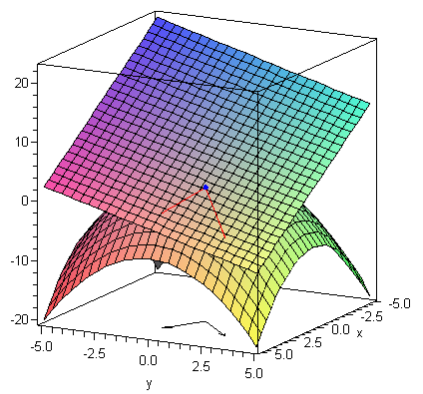
\includegraphics[width=\linewidth]{./Calculus/Images/6/Directional_Derivative_Example.png}
\end{image}%
\tcblower
\end{figureptx}%
\end{example}
To summarise:%
\begin{definition}{Directional Derivative.}{g:definition:id549877}%
The \emph{directional derivative} of the differentiable function \(f(x,y)\) at the point \((x_0,y_0)\) in the direction of the unit vector \(\hat{\bm{u}} = \langle u_1, u_2 \rangle\) is given by%
\begin{equation*}
D_{\bm{u}} f(x_0,y_0) = f_x(x_0,y_0)u_1 + f_y (x_0,y_0)u_2\text{.}
\end{equation*}
%
\end{definition}
\begin{example}{}{x:example:Ex-Find_Directional_Derivative}%
Find the directional derivative of \(f(x,y) = y\ln(x)\) at \((1,-3)\) in the direction \(\bm{u} = \langle -4, 3 \rangle\).%
\par\smallskip%
\noindent\textbf{\blocktitlefont Solution}.\hypertarget{g:solution:id549906}{}\quad{}For the given function%
\begin{equation*}
f_x = \dfrac{y}{x} \: \text{ and } \: f_y = \ln(x)\text{.}
\end{equation*}
Thus%
\begin{equation*}
f_x(1,-3) = -3 \: \text{ and } \: f_y(1,-3) = 0\text{.}
\end{equation*}
Now the unit vector in the direction of \(\langle -4,3 \rangle\) is%
\begin{equation*}
\hat{\bm{u}} = \left \langle -\dfrac{4}{5}, \dfrac{3}{5} \right \rangle\text{.}
\end{equation*}
Thus the required directional derivative is%
\begin{equation*}
D_{\hat{\bm{u}}} f(1,-3) = (-3) \left( -\dfrac{4}{5} \right) + (0) \left( \dfrac{3}{5} \right) = \dfrac{12}{5}\text{.}
\end{equation*}
%
\end{example}
\begin{example}{}{x:example:Ex-Find_Directional_Derivative_2}%
Find the directional derivative of \(f(x,y) = \sin(x+2y)\) in the direction of the angle (from the positive \(x\)-axis) \(\theta = \dfrac{3 \pi}{4}\).%
\par\smallskip%
\noindent\textbf{\blocktitlefont Solution}.\hypertarget{g:solution:id549945}{}\quad{}For the given function%
\begin{equation*}
f_x = \cos(x+2y) \: \text{ and } \: f_y = 2\cos(x+2y)\text{.}
\end{equation*}
Now, the unit vector in the direction of the angle \(\theta = \dfrac{3 \pi}{4}\) is%
\begin{equation*}
\hat{\bm{u}} = \left \langle - \dfrac{1}{\sqrt{2}}, \dfrac{1}{\sqrt{2}} \right \rangle\text{.}
\end{equation*}
Thus the required directional derivative is%
\begin{align*}
D_{\hat{\bm{u}}} f(x,y) \amp = \cos(x+2y) \left( - \dfrac{1}{\sqrt{2}} \right) + 2\cos(x+2y) \left( \dfrac{1}{\sqrt{2}} \right)\\
\amp = \dfrac{1}{\sqrt{2}} \cos(x+2y)
\end{align*}
%
\end{example}
Note that the directional derivative \(D_{\bm{u}} f(x_0,y_0)\) can be expressed in the terms of the scalar product if we use the following definition.%
\begin{definition}{Gradient Vector.}{g:definition:id549993}%
The vector%
\begin{equation*}
\nabla f(x_0,y_0) = \langle f_x(x_0,y_0), f_y(x_0,y_0) \rangle
\end{equation*}
is called the \emph{gradient vector} of \(f(x,y)\) at \((x_0,y_0)\).%
\end{definition}
With this definition the directional derivative can be written as:%
\begin{align*}
D_{\bm{u}} f(x_0,y_0) \amp = \langle f_x(x_0,y_0),f_y(x_0,y_0) \cdot \langle u_1, u_2 \rangle\\
\amp = \nabla f(x_0,y_0) \cdot \hat{\bm{u}}
\end{align*}
%
\begin{example}{}{x:example:Ex-Find_Gradient_Vector}%
Find the gradient vector for the function \(f(x,y) = e^{-x} \sin(y)\). Hence find \(\nabla f(0,\pi/3)\) and the directional derivative in the direction of the origin.%
\par\smallskip%
\noindent\textbf{\blocktitlefont Solution}.\hypertarget{g:solution:id550014}{}\quad{}For the given function%
\begin{equation*}
f_x = -e^{-x} \sin(y) \: \text{ and } \: f_y = e^{-x}\cos(y)\text{,}
\end{equation*}
and so the gradient vector is%
\begin{equation*}
\nabla f = \left \langle -e^{-x}\sin(y), e^{-x}\cos(y) \right \rangle\text{.}
\end{equation*}
Thus%
\begin{equation*}
\nabla f(0, \pi/3) = \left \langle -e^0 \sin \left( \dfrac{\pi}{3} \right), e^0 \cos \left( \dfrac{\pi}{3} \right) \right \rangle = \left \langle - \dfrac{\sqrt{3}}{2} , \dfrac{1}{2} \right \rangle\text{.}
\end{equation*}
Now, the unit vector in the direction of the origin from the point \(\left( 0, \dfrac{\pi}{3} \right)\) is%
\begin{equation*}
\hat{\bm{u}} = \langle 0, -1 \rangle\text{.}
\end{equation*}
Thus the required directional derivative is%
\begin{equation*}
D_{\hat{\bm{u}}} f \left( 0, \dfrac{\pi}{3} \right) = \left \langle -\dfrac{\sqrt{3}}{2} , \dfrac{1}{2} \right \rangle \cdot \langle 0, -1 \rangle = - \dfrac{1}{2}\text{.}
\end{equation*}
%
\end{example}
The gradient vector has some interesting facts associated with it. Note in the following we are assuming that \(\nabla f \neq \langle 0, 0 \rangle\).%
\par
%
\begin{enumerate}[label=\arabic*]
\item{}\(\nabla f\) points in the direction in which the directional derivative takes on its largest value. To see this, note that%
\begin{align*}
D_{\bm{u}} f(x,y) \amp = \nabla f(x,y) \cdot \hat{\bm{u}}\\
\amp = \| \nabla f \| \| \hat{\bm{u}} \| \cos(\theta)\\
\amp = \| \nabla f \| \cos(\theta)
\end{align*}
At a given point \(\| \nabla f \|\) is fixed and so the largest value of \(D_{\bm{u}} f(x,y)\) will occur when \(\cos(\theta) = 1\), i.e. when \(\theta = 0\) or put another way, when \(\hat{\bm{u}}\) is parallel to \(\nabla f\). We can also see from this that the largest value that the directional derivative can take is \(\| \nabla f \|\).%
\par
Similarly, the directional derivative takes on its smallest value in the direction of \(-\nabla f\) and has value \(- \| \nabla f \|\).%
\item{}\(\nabla f(x_0,y_0)\) is orthogonal (i.e. at right angles) to the level curve passing through \((x_0,y_0)\).%
\par
For the function \(z = f(x,y)\) the level curve passing through the point \((x_0,y_0)\) is given%
\begin{equation*}
f(x,y) = f(x_0,y_0)\text{.}
\end{equation*}
Now, as shown in Figure \hyperref[x:figure:Fig_tangent_vector]{Figure~{\xreffont\ref{x:figure:Fig_tangent_vector}}}, a vector parallel to the tangent to this curve at the point \((x_0,y_0)\) will be \(\left \langle 1, \dfrac{dy}{dx} \right \rangle\).%
\begin{figureptx}{}{x:figure:Fig_tangent_vector}{}%
\begin{image}{0.15}{0.7}{0.15}%
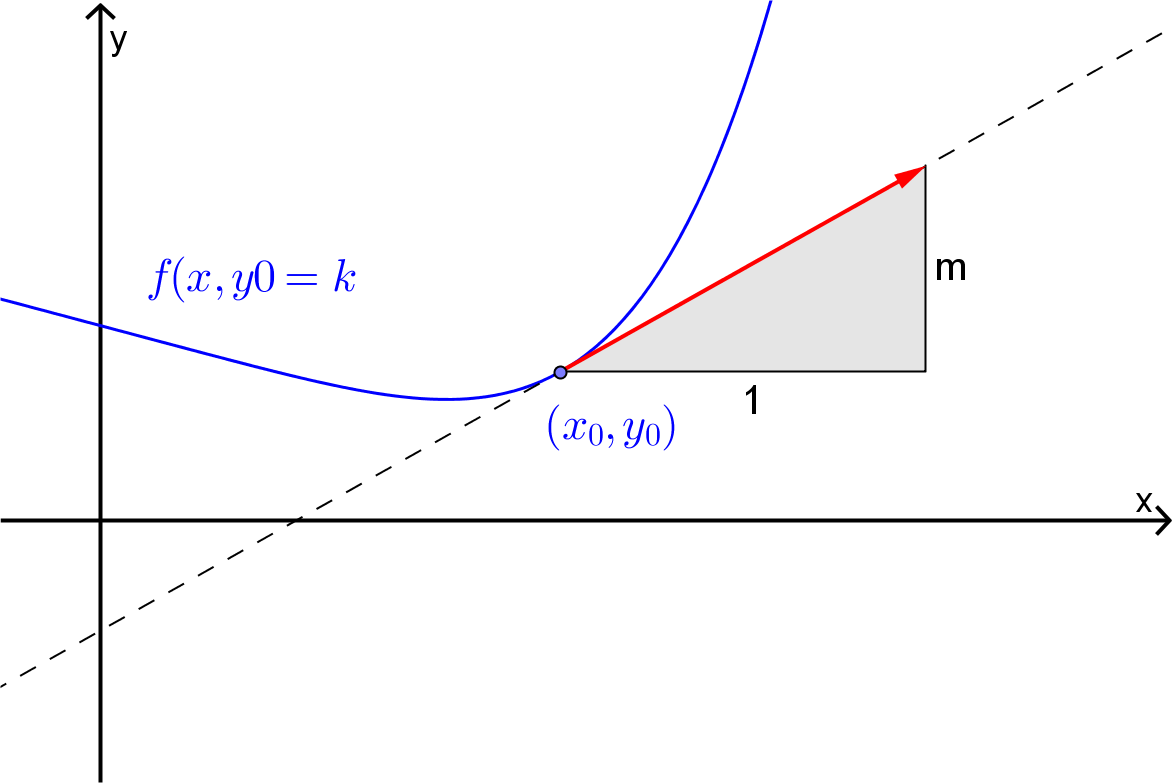
\includegraphics[width=\linewidth]{./Calculus/Images/6/Fig3_tangent_vector.png}
\end{image}%
\tcblower
\end{figureptx}%
Thus a vector normal to the curve at the point \((x_0,y_0)\) will be \(\left \langle \dfrac{f_x(x_0,y_0)}{f_y(x_0,y_0)}, 1 \right \rangle\), which is parallel to \(\nabla f(x_0,y_0)\).%
\par
Notice that since \(\nabla f(x_0,y_0)\) is orthogonal to the level curve passing through the point \((x_0,y_0)\) and that \(\nabla f (x_0,y_0)\) is the direction in which the directional derivative takes on its largest value, the ``path of steepest ascent'' on any surface \(z=f(x,y)\) is always at right angles to its contours. See the following diagram for an attempt to show this.%
\begin{figureptx}{}{x:figure:Fig_Contour_Plot}{}%
\begin{image}{0.15}{0.7}{0.15}%
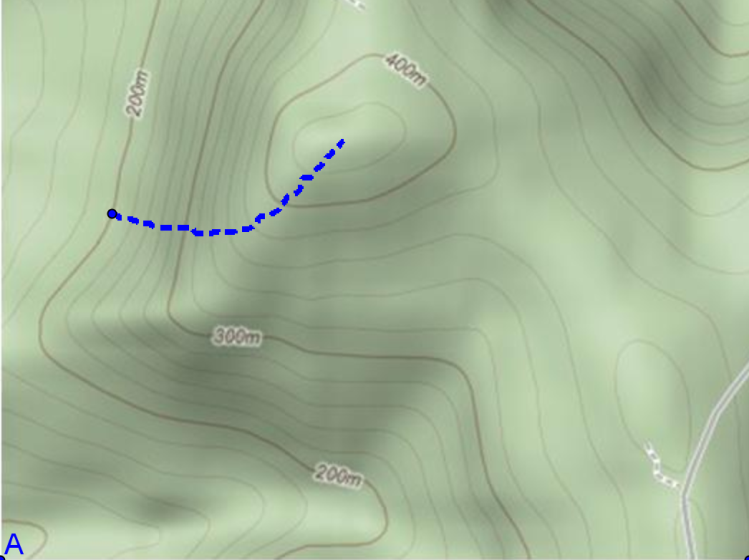
\includegraphics[width=\linewidth]{./Calculus/Images/6/Fig4_Contour_Plot.png}
\end{image}%
\tcblower
\end{figureptx}%
\end{enumerate}
%
\begin{example}{}{x:example:Ex-Find_Max_Min_Directional_Derivative}%
For the function \(f(x,y) = x^2y^3-3x\) find the directions in which the directional derivative at the point \((-2,4)\) is maximised, minimised and \(0\).%
\par\smallskip%
\noindent\textbf{\blocktitlefont Solution}.\hypertarget{g:solution:id550201}{}\quad{}For the given function%
\begin{equation*}
f_x = 2xy^3-3 \: \text{ and } \: f_y = 3x^2y^2\text{,}
\end{equation*}
and so%
\begin{equation*}
\nabla f(-2,4) = \langle -259,192 \rangle\text{.}
\end{equation*}
Thus the directional derivative, \(D_{\hat{\bm{u}}} f(-2,4)\), will be maximised in the direction%
\begin{equation*}
\bm{u} = \nabla f(-2,4) = \langle -259, 192 \rangle
\end{equation*}
and minimised in the direction%
\begin{equation*}
\bm{u} = -\nabla f(-2,4) = \langle 259, -192 \rangle\text{.}
\end{equation*}
Finally \(D_{\hat{\bm{u}}} f(-2,4)\) will be \(0\) when%
\begin{align*}
\nabla f(-2,4) \cdot \bm{u} \amp = 0\\
-259u_1 + 192u_2 \amp = 0
\end{align*}
i.e. when%
\begin{equation*}
\bm{u} = \langle 192, 259 \rangle
\end{equation*}
or some scalar multiple of this.%
\end{example}
\begin{example}{}{x:example:Ex-Find_lvlcurve_tanline_gradvec}%
For the function \(f(x,y) = x^2-y\) find the level curve, the tangent line and the gradient vector at the point \((-3,1)\).%
\par\smallskip%
\noindent\textbf{\blocktitlefont Solution}.\hypertarget{g:solution:id550232}{}\quad{}Since \(f(-3,1)=8\) the level curve through the point \((-3,1)\) is \(x^2-y=8\) or \(y=x^2-8\). We can find the equation of the tangent by standard calculus to obtain%
\begin{equation*}
y=-6x-17\text{.}
\end{equation*}
Next, the gradient vector is%
\begin{equation*}
\nabla f(-3,1) = \langle f_x(-3,1), f_y(-3,1) \rangle = \langle -6, -1 \rangle\text{.}
\end{equation*}
As can be seen in the diagram below, the gradient vector is orthogonal to the level curve.%
\begin{figureptx}{}{x:figure:Fig_gradvec_orthogonal_levelcurve}{}%
\begin{image}{0.15}{0.7}{0.15}%
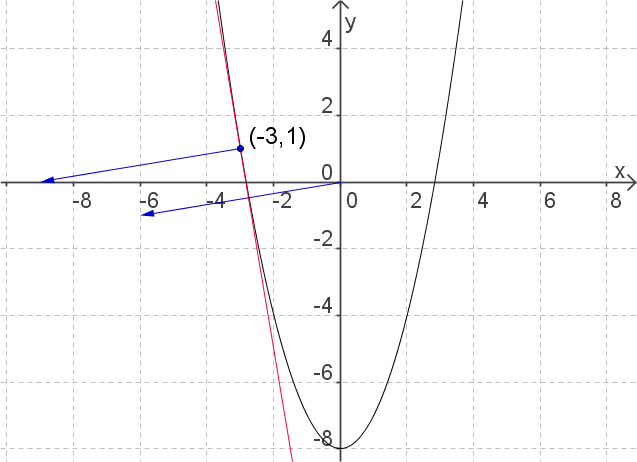
\includegraphics[width=\linewidth]{./Calculus/Images/6/Fig5_gradvec_orthogonal_levelcurve.png}
\end{image}%
\tcblower
\end{figureptx}%
\end{example}
\begin{example}{}{x:example:Ex-Hill_Climbing}%
Suppose you are climbing a hill whose shape is given by the equation%
\begin{equation*}
z = 1000-0.01x^2 - 0.02y^2
\end{equation*}
and you are standing at the point with coordinates \((60,100,764)\). %
\begin{enumerate}[label=\alph*]
\item{}In which direction should you proceed initially in order to be ascending most rapidly?%
\item{}If you climb in that direction, at what angle to the horizontal will you be climbing initially?%
\end{enumerate}
%
%
\par\smallskip%
\noindent\textbf{\blocktitlefont Solution}.\hypertarget{g:solution:id550336}{}\quad{}%
\begin{enumerate}[label=\alph*]
\item{}Since we want to travel on the path of steepest ascent we will want to head in the direction of \(\nabla f(60,100)\). Now%
\begin{equation*}
\nabla f(x,y) = \langle -0.02x, -0.04y \rangle
\end{equation*}
and hence%
\begin{equation*}
\nabla f (60,100) = \langle-1.2,-4 \rangle\text{.}
\end{equation*}
%
\item{}In this direction we know that%
\begin{equation*}
D_{\hat{\bm{u}}} f(60,100) = \| \nabla f(60,100) \| \simeq 4.17\text{.}
\end{equation*}
Thus the angle, \(\theta\), to the horizontal will be%
\begin{equation*}
\theta = \tan^{-1} (4.17) \simeq 1.33^{c}\text{.}
\end{equation*}
%
\end{enumerate}
%
\end{example}
%
%
\typeout{************************************************}
\typeout{Exercises 6.1 Example Tasks}
\typeout{************************************************}
%
\begin{exercises-subsection-numberless}{Example Tasks}{}{Example Tasks}{}{}{g:exercises:id550350}
\begin{divisionexercise}{1}{}{}{g:exercise:id550352}%
Find the directional derivative for \(f(x,y) = (x-2y)^2 + 5x^2\) at the point \((-3,1)\) in the direction of the point \((1,4)\).%
\end{divisionexercise}%
\begin{divisionexercise}{2}{}{}{g:exercise:id548130}%
Find the maximum value of the rate of change of \(h(s,t) = \dfrac{1}{\sqrt{s^2+t^2}}\) at \((3,4)\).%
\end{divisionexercise}%
\begin{divisionexercise}{3}{}{}{g:exercise:id548151}%
For the curve \(e^x \ln (y) - xy = 0\) use the gradient vector of a two variable function to find the tangent line and the normal line at the point \((2,e^2)\).%
\end{divisionexercise}%
\begin{divisionexercise}{4}{}{}{g:exercise:id548122}%
For the following contour plot for some unspecified function of two variables estimate the sign of the directional derivatives at:%
\begin{figureptx}{}{x:figure:ET_Contour_Plot}{}%
\begin{image}{0.15}{0.7}{0.15}%
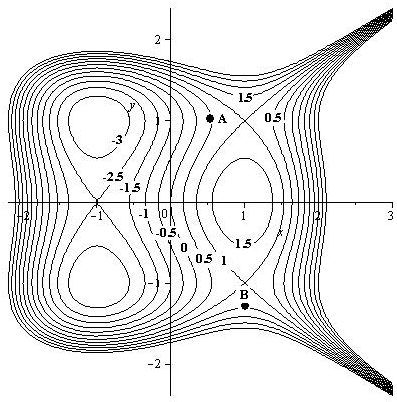
\includegraphics[width=\linewidth]{./Calculus/Images/6/Example-Task-4_Contour_Plot.png}
\end{image}%
\tcblower
\end{figureptx}%
%
\begin{enumerate}[label=\alph*]
\item{}The point \(A\) and in the direction of \(\bm{u} = \langle 1,2 \rangle\).%
\item{}The point \(B\) and in the direction of \(\bm{w} = \langle -1,-1 \rangle\).%
\item{}The point \(A\) and in the direction of the origin.%
\item{}The point \(B\) and in the direction of the origin.%
\end{enumerate}
%
\end{divisionexercise}%
\end{exercises-subsection-numberless}
\end{sectionptx}
%
%
\typeout{************************************************}
\typeout{Section 6.2 In Three Variables}
\typeout{************************************************}
%
\begin{sectionptx}{In Three Variables}{}{In Three Variables}{}{}{x:section:In_Three_Variables}
The concepts of the directional derivative and the gradient vector extend to functions of more than two variables. In this section we will look at some examples for functions of three variables.%
\begin{example}{}{x:example:Ex-rate_of_change}%
Find the rate of change of the function \(f(x,y,z) = xy+yz^2+xz^3\) at the point \((2,0,3)\) in the direction \(\hat{\bm{u}} = \left \langle -\dfrac{2}{3}, -\dfrac{1}{3}, \dfrac{2}{3} \right \rangle\).%
\par\smallskip%
\noindent\textbf{\blocktitlefont Solution}.\hypertarget{g:solution:id551932}{}\quad{}The gradient vector for the given function is%
\begin{align*}
\nabla f \amp = \left \langle f_x, f_y, f_z \right \rangle\\
\amp = \left \langle y +z^3, x+z^2, 2yz+3xz^2 \right \rangle\text{.}
\end{align*}
Thus%
\begin{equation*}
\nabla f (2,0,3) = \langle 27, 11, 54 \rangle
\end{equation*}
and so the required directional derivative is%
\begin{equation*}
D_{\hat{\bm{u}}} f(2,0,3) = \langle 27, 11, 54 \rangle \cdot \left \langle -\dfrac{2}{3}, -\dfrac{1}{3}, \dfrac{2}{3} \right \rangle = \dfrac{43}{3}\text{.}
\end{equation*}
%
\end{example}
\begin{example}{}{x:example:Ex-Temperature}%
The temperature at the point \((x,y,z)\) is given by the function%
\begin{equation*}
T(x,y,z) = 200e^{-x^2-3y^2-9z^2}\text{.}
\end{equation*}
%
\begin{enumerate}[label=\alph*]
\item{}Find the rate of change of temperature at the point \(P = (2,-1,2)\) in the direction \(\overrightarrow{PQ}\) where \(Q = (3,-3,3)\).%
\item{}In which direction does the temperature increase the fastest at \(P\)?%
\item{}Find the maximum rate of increase at \(P\).%
\end{enumerate}
%
%
\par\smallskip%
\noindent\textbf{\blocktitlefont Solution}.\hypertarget{g:solution:id552020}{}\quad{}The gradient vector for the given function is%
\begin{align*}
\nabla T \amp = \left \langle T_x, T_y, T_z \right \rangle\\
\amp = \left \langle -400xe^{-x^2-3y^2-9z^2}, -1200ye^{-x^2-3y^2-9z^2},-3600ze^{-x^2-3y^2-9z^2} \right \rangle\text{.}
\end{align*}
Thus%
\begin{equation*}
\nabla T (2,-1,2) = 400e^{-43} \langle -2, 3, -18 \rangle\text{.}
\end{equation*}
%
\par
%
\begin{enumerate}[label=\alph*]
\item{}Since \(\overrightarrow{PQ} = \langle 1, -2, 1 \rangle\), the required rate of change is given by the directional derivative%
\begin{equation*}
D_{\hat{\bm{u}}} T(2,-1,2) = 400 e^{-43} \langle -2, 3, -18 \rangle \cdot \dfrac{1}{\sqrt{6}} \langle 1, -2, 1 \rangle = \dfrac{-10400}{\sqrt{6}} e^{-43}\text{.}
\end{equation*}
%
\item{}The direction in which the temperature increase the fastest at \(P\) is%
\begin{equation*}
\nabla T (2,-1,2) = 400e^{-43} \langle -2, 3, -18 \rangle\text{.}
\end{equation*}
%
\item{}The maximum rate of increase at \(P\) is the maximum value of \(D_{\bm{u}} T(2,-1,2)\) which is%
\begin{equation*}
\| \nabla T (2,-1,2) \| = \dfrac{400 \sqrt{337}}{e^{43}}\text{.}
\end{equation*}
%
\end{enumerate}
%
\end{example}
\begin{example}{}{x:example:Ex-Level_surface_equation}%
Find the equation of the tangent plane to the level surface of \(f(x,y,z) = x^2+y^2 - z + \cos(z)\) at the point \((-1,1,0)\).%
\par\smallskip%
\noindent\textbf{\blocktitlefont Solution}.\hypertarget{g:solution:id552102}{}\quad{}Since \(f(-1,1,0) = 3\), the level surface for this function satisfies the equation%
\begin{equation*}
x^2+y^2 - z + \cos(z) = 3\text{.}
\end{equation*}
A normal to this surface at the point \((-1,1,0)\), and hence to the tangent plane at this point, is given by \(\nabla f (-1,1,0)\). Now,%
\begin{equation*}
\nabla f = \left \langle 2x, 2y, -1-\sin(z) \right \rangle\text{,}
\end{equation*}
and so%
\begin{equation*}
\nabla f (-1,1,0) = \langle-2, 2, -1 \rangle\text{.}
\end{equation*}
Thus the equation of the tangent plane is%
\begin{equation*}
\langle -2, 2, -1 \rangle \cdot \left( \langle x, y, z \rangle - \langle -1, 1, 0 \rangle \right) = 0
\end{equation*}
which simplifies to%
\begin{equation*}
2x-2y+z = -4\text{.}
\end{equation*}
%
\end{example}
%
%
\typeout{************************************************}
\typeout{Exercises 6.2 Example Tasks}
\typeout{************************************************}
%
\begin{exercises-subsection-numberless}{Example Tasks}{}{Example Tasks}{}{}{g:exercises:id552147}
\begin{divisionexercise}{1}{}{}{g:exercise:id552125}%
Find the directional derivative of \(g(x,y,z) = \dfrac{z-x}{z+y}\) at \((1,0,-3)\) in the direction \(\bm{a} = -6\bm{i} + 3\bm{j} - 2\bm{k}\).%
\end{divisionexercise}%
\begin{divisionexercise}{2}{}{}{g:exercise:id552146}%
By thinking of level surfaces to a function of 3 variables show that the normal lines to a sphere pass through its centre.%
\end{divisionexercise}%
\end{exercises-subsection-numberless}
\end{sectionptx}
\end{chapterptx}
 %
%
\typeout{************************************************}
\typeout{Chapter 7 Local and Global Extrema}
\typeout{************************************************}
%
\begin{chapterptx}{Local and Global Extrema}{}{Local and Global Extrema}{}{}{x:chapter:Calculus_7}
%
%
\typeout{************************************************}
\typeout{Section 7.1 Critical Points}
\typeout{************************************************}
%
\begin{sectionptx}{Critical Points}{}{Critical Points}{}{}{x:section:Critical-Points}
Recall  that  a  function  of  one  variable, \(f(x)\)  has  a  ``critical  point'' at \(x=x_0\) if  the tangent line to the curve at \(x=x_0\) is horizontal or if the derivative does not exist at that point. This critical point can be either a (local) maximum, minimum or horizontal point of inflection or vertical point of inflection.  (The first three possibilities are shown in Figure \hyperref[x:figure:Fig_max_min_inflection]{Figure~{\xreffont\ref{x:figure:Fig_max_min_inflection}}} below.)%
\begin{figureptx}{}{x:figure:Fig_max_min_inflection}{}%
\begin{image}{0.15}{0.7}{0.15}%
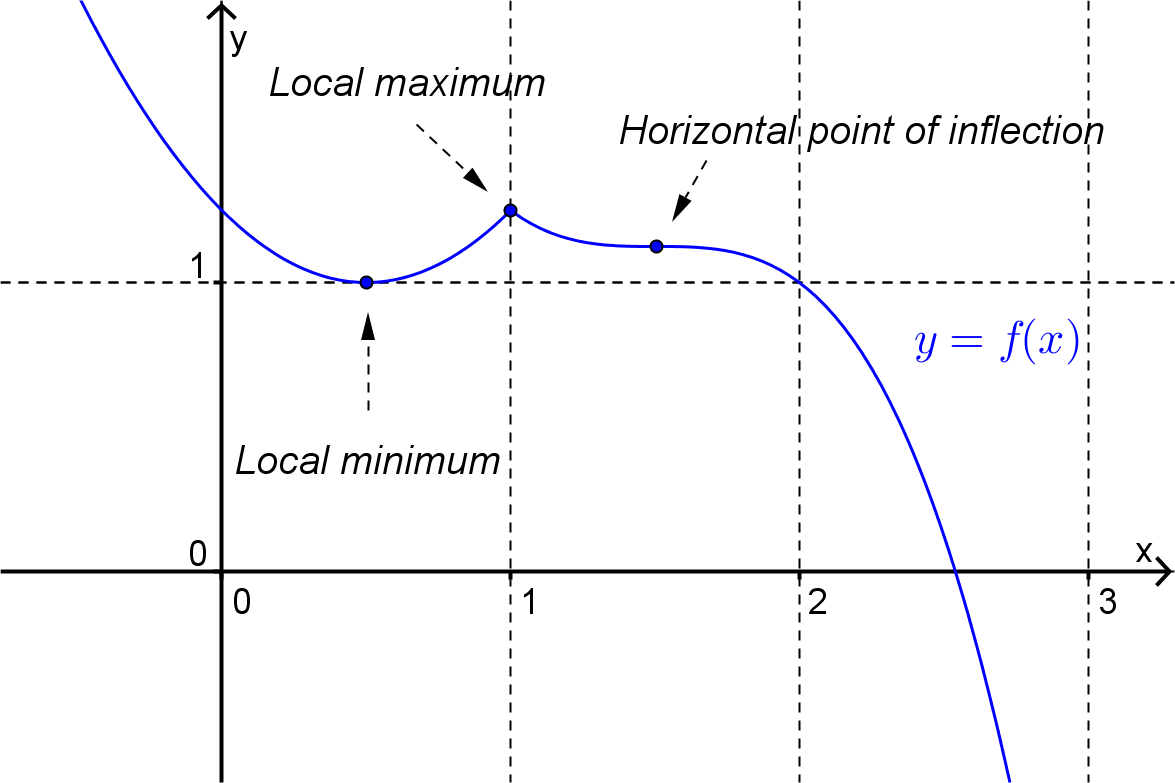
\includegraphics[width=\linewidth]{./Calculus/Images/7/Fig1_max_min_inflection.png}
\end{image}%
\tcblower
\end{figureptx}%
The idea of critical points can be applied to functions of two variables.%
\begin{definition}{Critical Point.}{g:definition:id552257}%
The function \(z=f(x,y)\) has a \emph{critical point} at \((x_0,y_0)\) if the tangent plane to the surface at the point \((x_0,y_0,z_0)\) is horizontal or if one of the directional derivatives does not exist.%
\end{definition}
As with functions of one variable, critical points of functions of two variables will be one of three types.%
\par
%
\begin{enumerate}[label=\arabic*]
\item{}If at a critical point \(f(x,y) \leq f(x_0,y_0)\) for all points in some open disk centred on \((x_0,y_0)\) then the critical point is a \alert{local maximum}.%
\item{}If at a critical point \(f(x,y) \geq f(x_0,y_0)\) for all points in some open disk centred on \((x_0,y_0)\) then the critical point is a \alert{local minimum}.%
\item{}For a smooth function (i.e. a function for which all derivatives exist) if a critical point is not a local maximum or a local minimum then it is a \alert{saddle point}.%
\end{enumerate}
%
\begin{example}{}{x:example:Ex-Local_max_and_min}%
The graph of the function%
\begin{equation*}
f(x,y) = x(5x+2)(3y-2)e^{-\left( \frac{x^2+y^2}{5} \right)}
\end{equation*}
is given below with local maxima and local minima labelled.%
\begin{figureptx}{}{x:figure:Fig_Local_max_min}{}%
\begin{image}{0.05}{0.9}{0.05}%
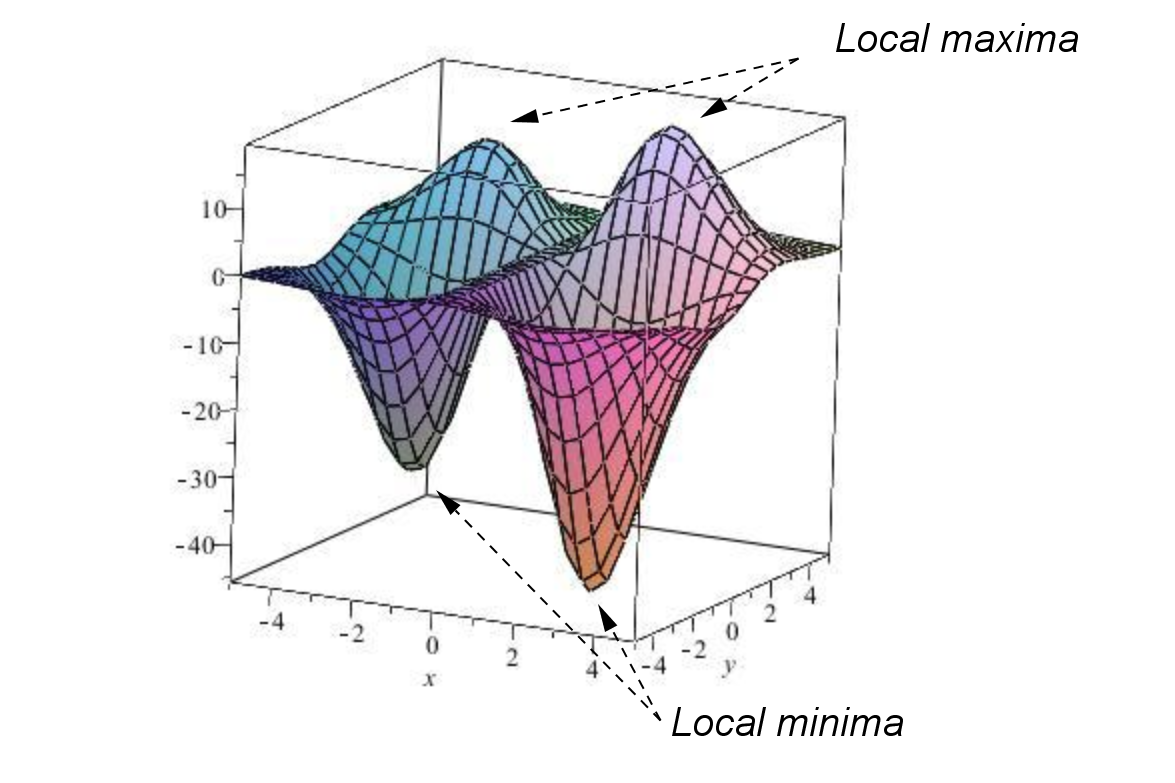
\includegraphics[width=\linewidth]{./Calculus/Images/7/Fig2_Local_max_and_min.png}
\end{image}%
\tcblower
\end{figureptx}%
\end{example}
\begin{example}{}{x:example:Ex-Saddle_point}%
The graph of the function \(f(x,y) = x^2-y^2\) is given below with a saddle point labelled.%
\begin{figureptx}{}{x:figure:Fig_Saddle_point}{}%
\begin{image}{0.05}{0.9}{0.05}%
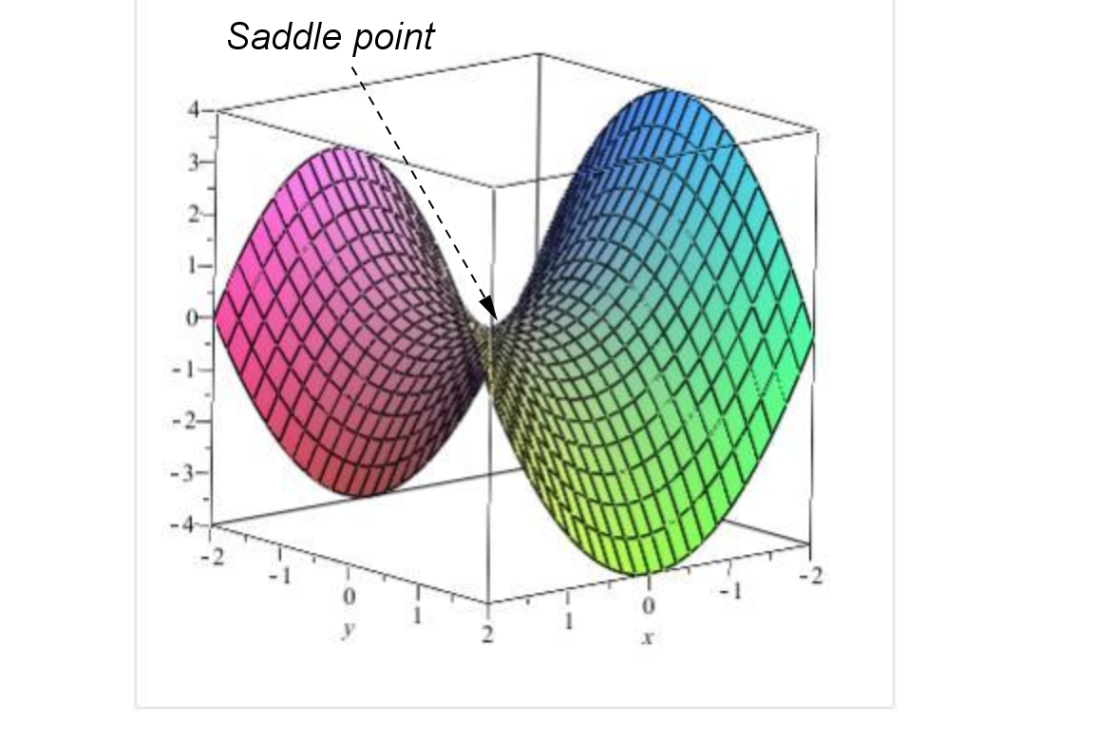
\includegraphics[width=\linewidth]{./Calculus/Images/7/Fig3_Saddle_point.png}
\end{image}%
\tcblower
\end{figureptx}%
\end{example}
For smooth functions we can find the critical points by looking for those points where the tangent plane is horizontal. If the function \(z=f(x,y)\) has a tangent plane at the point \((x_0,y_0,z_0)\) we can determine algebraically that it is horizontal by checking that:%
\par
%
\begin{itemize}[label=\textbullet]
\item{}The normal vector for the plane is parallel to the vector \(\langle 0,0,1 \rangle\), or%
\item{}The directional derivative at \((x_0,y_0)\) is zero in every direction, or%
\item{}The gradient vector at \((x_0,y_0)\) is \(\langle 0,0 \rangle\).%
\end{itemize}
%
\par
These conditions are all equivalent and they lead us to the following theorem.%
\begin{theorem}{Critical Point.}{}{g:theorem:id552377}%
The point \((x_0,y_0)\) is a critical point of the function \(z = f(x,y)\) if%
\begin{equation*}
f_x(x_0,y_0) = f_y (x_0,y_0) = 0\text{,}
\end{equation*}
or, if at least one of these derivatives does not exist.%
\end{theorem}
\alert{Note:} For the most part, we will assume that the function is smooth, i.e. has derivatives of all orders.  In particular a smooth function does not have any discontinuities or cusps. Such critical points will occur for functions of two variables when at least one of the partial derivatives does not exist at the critical point.%
\begin{example}{}{x:example:Ex-Locate_critical_points}%
Locate, and determine the nature of, the critical points of the function%
\begin{equation*}
z = 2x^3 + (x+1)y^2 + 5x^2\text{.}
\end{equation*}
%
\par\smallskip%
\noindent\textbf{\blocktitlefont Solution}.\hypertarget{g:solution:id552390}{}\quad{}To locate the critical points we solve the equations \(z_x = z_y = 0\), and check for any points where they do not exist. Since this function is given by a polynomial, the partial derivatives exist.  We set them to zero below.%
\begin{align}
6x^2 + y^2 + 10x \amp = 0\label{x:mrow:Eq-Partial_eq1}\\
2(x+1)y \amp = 0\label{x:mrow:Eq-Partial_eq2}
\end{align}
From \hyperref[x:mrow:Eq-Partial_eq2]{({\xreffont\ref{x:mrow:Eq-Partial_eq2}})}%
\begin{equation*}
x=-1 \: \text{ or } \: y=0\text{.}
\end{equation*}
Putting \(y=0\) into \hyperref[x:mrow:Eq-Partial_eq1]{({\xreffont\ref{x:mrow:Eq-Partial_eq1}})} gives%
\begin{equation*}
x=0 \: \text{ or } \: x=-\dfrac{5}{3}\text{.}
\end{equation*}
Putting \(x=-1\) into \hyperref[x:mrow:Eq-Partial_eq1]{({\xreffont\ref{x:mrow:Eq-Partial_eq1}})} gives%
\begin{equation*}
y=2 \: \text{ or } \: y=-2\text{.}
\end{equation*}
Thus there are 4 critical points at%
\begin{equation*}
\left( 0, 0 \right), \left( -\dfrac{5}{3}, 0 \right), \left( -1, 2 \right) \: \text{ and } \left( -1, -2 \right)\text{.}
\end{equation*}
%
\par
If we have the graph of the function then we can usually determine the nature of these critical points by inspection. From the (computer generated) graph shown below we can see with very careful inspection that the critical point at \((0,0)\) is a local minimum, the critical point at \(\left( -\dfrac{5}{3}, 0 \right)\) is a local maximum and the critical points at \((-1,2)\) and \((-1,-2)\) are saddle points.%
\begin{figureptx}{}{x:figure:Fig-Locate_critical_points}{}%
\begin{image}{0.1}{0.8}{0.1}%
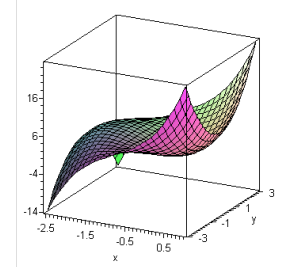
\includegraphics[width=\linewidth]{./Calculus/Images/7/Fig4-Locate_critical_points.png}
\end{image}%
\tcblower
\end{figureptx}%
Sometimes the nature of the critical points is not clear on such graphs or we don’t have access to the graph. Another approach to determining the nature of the critical points is to sketch the level curves for the function.%
\begin{figureptx}{}{x:figure:Fig-Locate_critical_points2}{}%
\begin{image}{0.1}{0.8}{0.1}%
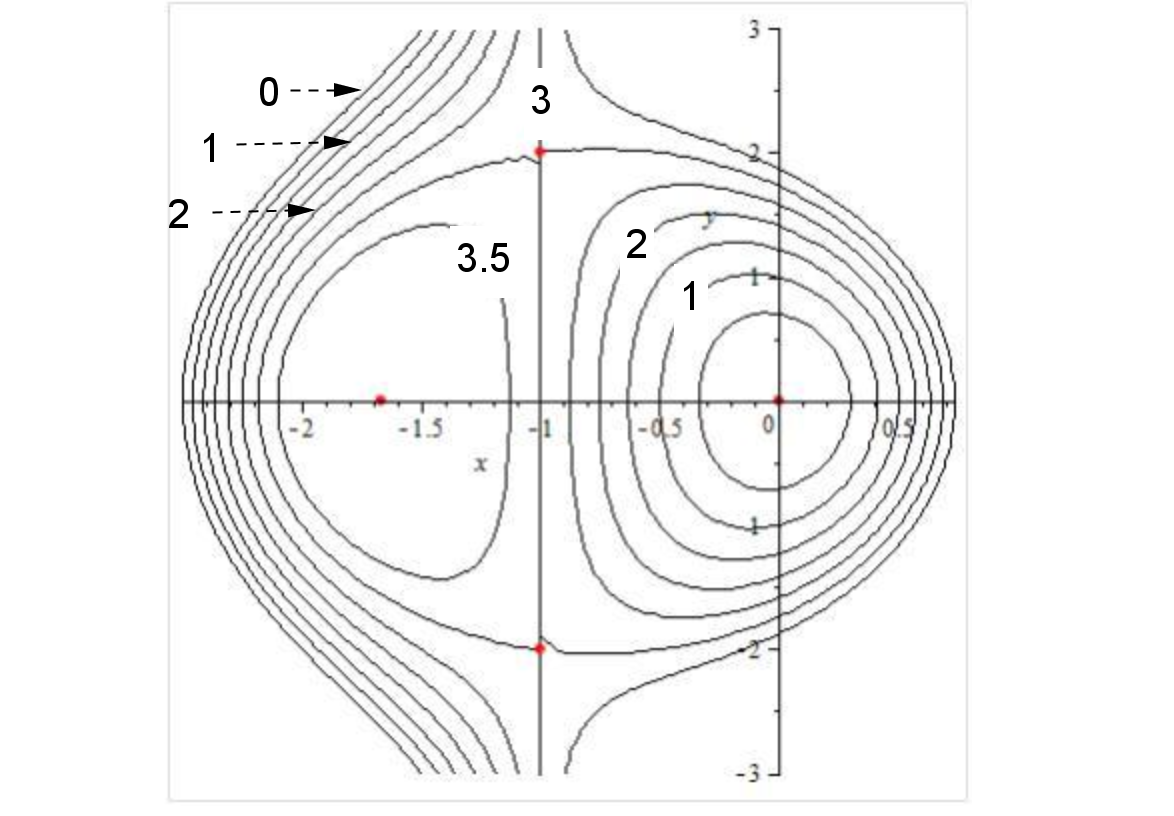
\includegraphics[width=\linewidth]{./Calculus/Images/7/Fig5-Locate_critical_points.png}
\end{image}%
\tcblower
\end{figureptx}%
From this diagram we can see that as we move away from the critical points at \(\left(0,0\right)\) in any direction the function value is increasing and hence \(\left(0,0\right)\) is local minimum. Similarly as we move away from the critical point at \(\left(-\dfrac{5}{3},0\right)\) in any direction the function value is decreasing is hence \(\left(-\dfrac{5}{3},0\right)\) is a local maximum. For the critical points at \(\left(-1,2\right)\) and \(\left(-1,-2\right)\) we can move away in some directions and have the function value increase while in other directions the function value will decrease. Hence these critical points are saddle points.%
\end{example}
%
%
\typeout{************************************************}
\typeout{Exercises 7.1 Example Tasks}
\typeout{************************************************}
%
\begin{exercises-subsection-numberless}{Example Tasks}{}{Example Tasks}{}{}{g:exercises:id552518}
\begin{divisionexercise}{1}{}{}{g:exercise:id552531}%
Find the critical points of the function \(f(x,y) = 3x-x^3-2y^2+y^4\) and use the plot of level curves given below to determine the nature of each critical point.%
\begin{figureptx}{}{x:figure:Fig-Ex_task_section_1}{}%
\begin{image}{0.1}{0.8}{0.1}%
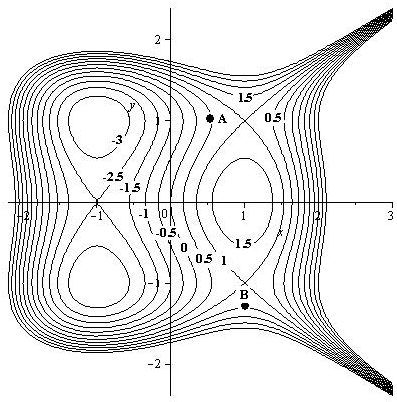
\includegraphics[width=\linewidth]{./Calculus/Images/7/Ex_task_section_1.png}
\end{image}%
\tcblower
\end{figureptx}%
\end{divisionexercise}%
\end{exercises-subsection-numberless}
\end{sectionptx}
%
%
\typeout{************************************************}
\typeout{Section 7.2 Second Derivative Test}
\typeout{************************************************}
%
\begin{sectionptx}{Second Derivative Test}{}{Second Derivative Test}{}{}{x:section:Second-Derivative-Test}
An algebraic method for determining what type of critical points a function has is given by the following theorem.%
\begin{theorem}{The Second Derivative Test.}{}{g:theorem:id552568}%
Let the function \(z=f(x,y)\) have continuous 2nd partial derivatives and let \((x_0,y_0)\) be a critical point of the function. Let%
\begin{equation*}
D = f_{xx} (x_0,y_0) f_{yy} (x_0,y_0) - \left[ f_{xy} (x_0,y_0) \right]^2\text{.}
\end{equation*}
%
\par
%
\begin{itemize}[label=\textbullet]
\item{}If \(D>0\) and \(f_{xx} (x_0,y_0) >0\) then \(f\) has a local minimum at \((x_0,y_0)\).%
\item{}If \(D>0\) and \(f_{xx} (x_0,y_0) < 0\) then \(f\) has a local maximum at \((x_0,y_0)\).%
\item{}If \(D < 0\) then \(f\) has a saddle point at \((x_0,y_0)\).%
\item{}If \(D=0\) then the 2nd derivative test is inconclusive.%
\end{itemize}
%
\end{theorem}
\alert{Outline of Proof:} For the sake of simplicity assume that the critical point is at the point \((x_0,y_0)=(0,0)\). Now using a Taylor expansion for functions of two variables about \((a,b) = (0,0)\) we have (up to the quadratic terms)%
\begin{equation*}
f(x,y); f(0,0) + f_x (0,0)x + f_y (0,0) y + \dfrac{f_{xx}(0,0)}{2} x^2 + f_{xy} (0,0) xy + \dfrac{f_{yy}(0,0)}{2} y^2\text{.}
\end{equation*}
Since \((x_0,y_0) = (0,0)\) is a critical point of the function \(f_x (0,0) = f_y (0,0) = 0\). Thus%
\begin{equation*}
f(x,y); f(0,0) + \dfrac{f_{xx}(0,0)}{2}x^2 + f_{xy} (0,0) xy + \dfrac{f_{yy} (0,0)}{2}y^2\text{.}
\end{equation*}
%
\par
On completing the square (and dropping the evaluation at \((0,0)\) for brevity)%
\begin{align*}
f(x,y) \amp \simeq f + \dfrac{f_{xx}}{2} \left \{x^2 + \dfrac{2f_{xy}}{f_{xx}} + \left( \dfrac{f_{xy}}{f_{xx}} \right)^2 y^2 \right \} - \dfrac{f_{xx}}{2} \left( \dfrac{f_{xy}}{f_{xx}} \right)^2 y^2 + \dfrac{f_{yy}}{2}y^2\\
\amp = f + \dfrac{f_{xx}}{2} \left( x + \dfrac{f_{xy}}{f_{xx}} y \right)^2 + \dfrac{1}{2 f_{xx}} y^2 \left( f_{xx} f_{yy} - f_{xy}^2 \right)\text{.}
\end{align*}
%
\par
From this we can see that if \(f_{xx} > 0\) and \(D = f_{xx} f_{yy} - f_{xy}^2 > 0\) then when \(x\) and \(y\) are varied from \((0,0)\), \(f(x,y)\) increases and so \((x_0,y_0) = (0,0)\) will be a local minimum.%
\begin{example}{}{x:example:Ex-Locate_critical_points_2}%
Locate and identify the critical points of the function \(f(x,y) = 2x^3 + (x+1)y^2 + 5x^2\).%
\par\smallskip%
\noindent\textbf{\blocktitlefont Solution}.\hypertarget{g:solution:id552652}{}\quad{}We located the critical points of this function in an earlier example. We found that there are 4 critical points at%
\begin{equation*}
\left( 0, 0 \right), \left( -\dfrac{5}{3}, 0 \right), \left( -1, 2 \right) \: \text{ and } \left( -1, -2 \right)\text{.}
\end{equation*}
%
\par
To determine the nature of these critical points, in this example we will use the second derivative test. To this end, note that%
\begin{equation*}
f_{xx} = 12x+10, \: f_{xy} = 2y, \: \text{ and } f_{yy} = 2x+2\text{.}
\end{equation*}
Thus%
\begin{align*}
D \amp = f_{xx} f_{yy} - f_{xy}^2 = (12x+10)(2x+2) - (2y)^2\\
\amp = 24x^2 + 44x -4y^2+20\text{.}
\end{align*}
Now, applying the second derivative test:%
\par
%
\begin{itemize}[label=\textbullet]
\item{}At \((0,0)\), \(D=20>0\), \(f_{xx}=10>0\) and so \((0,0)\) is a local minimum.%
\item{}At \((-\dfrac{5}{3},0)\), \(D=\dfrac{40}{3}>0\), \(f_{xx}=-10 < 0\) and so \((-\dfrac{5}{3},0)\) is a local maximum.%
\item{}At \((-1,2)\), \(D=-16 < 0\) and so \((-1,2)\) is a saddle point.%
\item{}At \((-1,-2)\), \(D=-16 < 0\) and so \((-1,-2)\) is also a saddle point.%
\end{itemize}
%
\par
This is in agreement with the conclusions we made on the nature of these critical pointson the basis of the level curves of the function.%
\end{example}
\begin{example}{}{x:example:Ex-Locate_critical_points_3}%
Locate and identify the critical points of the function%
\begin{equation*}
g(x,y) = 2 - \sqrt{x^2+y^2}\text{.}
\end{equation*}
%
\par\smallskip%
\noindent\textbf{\blocktitlefont Solution}.\hypertarget{g:solution:id552780}{}\quad{}Here%
\begin{equation*}
g_x = \dfrac{-x}{\sqrt{x^2+y^2}} \: \text{ and } \: g_y = \dfrac{-y}{\sqrt{x^2+y^2}}\text{.}
\end{equation*}
%
\par
For this function both partial derivatives are undefined at \((x, y) = (0,0)\) and so this point will be a critical point. However we cannot use the second derivative test to determine the nature of this critical point. In this case we can see from the graph of the function that the critical point at \((x, y) = (0,0)\) is a local maximum.%
\begin{figureptx}{}{x:figure:Fig-Loc_and_identify_critical_points}{}%
\begin{image}{0.15}{0.7}{0.15}%
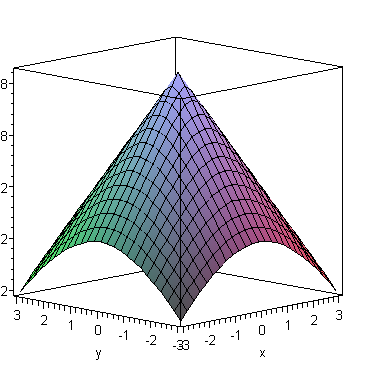
\includegraphics[width=\linewidth]{./Calculus/Images/7/Fig6_Loc_and_identify_critical_points.png}
\end{image}%
\tcblower
\end{figureptx}%
\end{example}
%
%
\typeout{************************************************}
\typeout{Exercises 7.2 Example Tasks}
\typeout{************************************************}
%
\begin{exercises-subsection-numberless}{Example Tasks}{}{Example Tasks}{}{}{g:exercises:id552830}
\begin{divisionexercise}{1}{}{}{g:exercise:id552827}%
Locate and identify the critical points of the function \(z=3x-x^3-2y^2+y^4\).%
\end{divisionexercise}%
\begin{divisionexercise}{2}{}{}{g:exercise:id552838}%
Locate and identify the critical points of the function \(z=\exp \left(xy-\frac{2}{3}x^2 - \frac{2}{3}y^3 \right)\).%
\begin{figureptx}{}{x:figure:Ex2_crit_points}{}%
\begin{image}{0.15}{0.7}{0.15}%
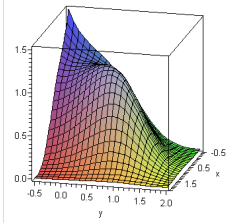
\includegraphics[width=\linewidth]{./Calculus/Images/7/Ex2_crit_points.png}
\end{image}%
\tcblower
\end{figureptx}%
\end{divisionexercise}%
\end{exercises-subsection-numberless}
\end{sectionptx}
%
%
\typeout{************************************************}
\typeout{Section 7.3 Global Extrema}
\typeout{************************************************}
%
\begin{sectionptx}{Global Extrema}{}{Global Extrema}{}{}{x:section:Global-Extrema}
\begin{definition}{Global Extrema.}{g:definition:id552845}%
Consider the function of two variables \(f(x,y)\) on the domain D.%
\par
%
\begin{itemize}[label=\textbullet]
\item{}If there exists some point \((x_0,y_0)\) in \(D\) such that \(f(x,y) \leq f(x_0,y_0)\) for all points \((x,y)\) in \(D\) then the function has a \emph{global maximum} at \((x_0,y_0)\).%
\item{}Similarly, if there exists some point \((x_0,y_0)\) in \(D\) such that \(f(x,y) \geq f(x_0,y_0)\) for all points \((x,y)\) in \(D\) then the function has a \emph{global minimum} at \((x_0,y_0)\).%
\end{itemize}
%
\end{definition}
\begin{example}{}{g:example:id552953}%
The graph of the function%
\begin{equation*}
f(x,y) = x(5x+2)(3y-2)e^{-\left( \dfrac{x^2+y^2}{5} \right)}
\end{equation*}
over the domain \(D = \left \{ (x,y): -5 \leq x \leq 5, \, -5 \leq y \leq 5 \right \}\) is shown below.%
\begin{figureptx}{}{x:figure:Fig7_Global_Extrema}{}%
\begin{image}{0.1}{0.8}{0.1}%
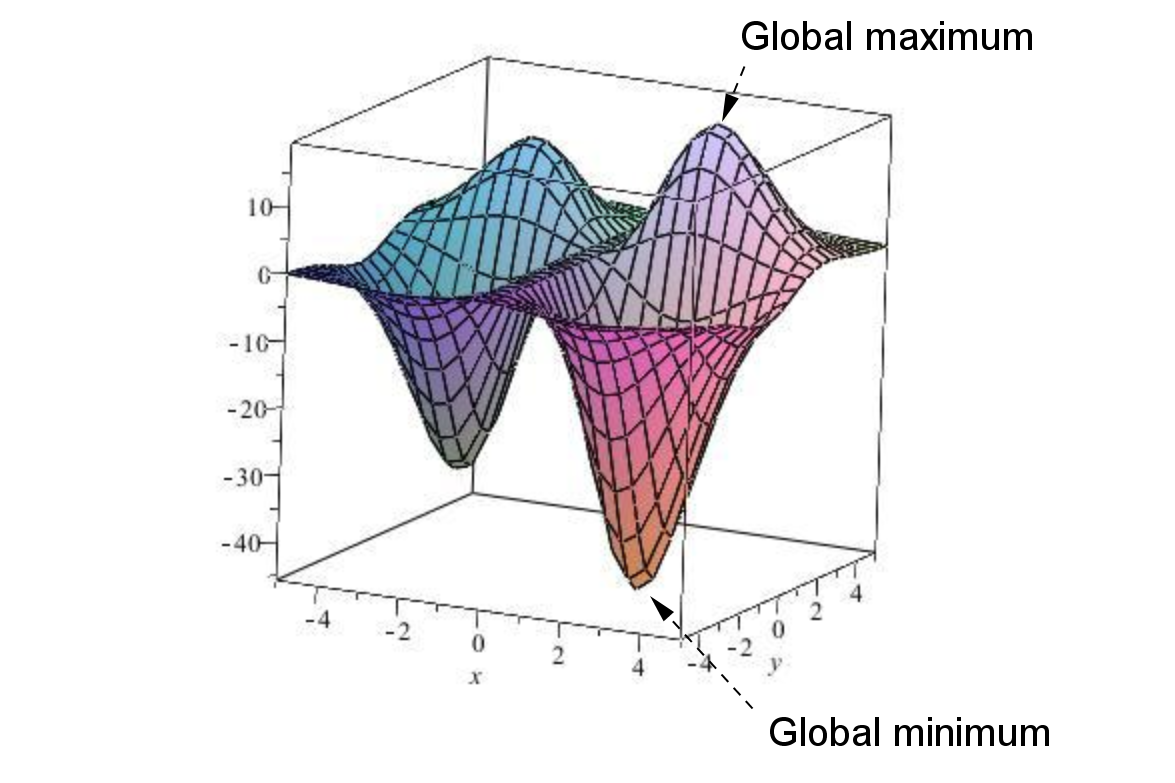
\includegraphics[width=\linewidth]{./Calculus/Images/7/Fig7_Global_Extrema.png}
\end{image}%
\tcblower
\end{figureptx}%
\end{example}
Before discussing global extrema for functions of two variables, recall the situation for a function of one variable \(y=f(x)\). If \(f(x)\) is continuous on the closed interval \(I=[a,b]\) then \(f(x)\) is guaranteed to have both a global maximum and a global minimum on \(I\).%
\begin{figureptx}{}{x:figure:Fig8_Global_Extrema_1D}{}%
\begin{image}{0.1}{0.8}{0.1}%
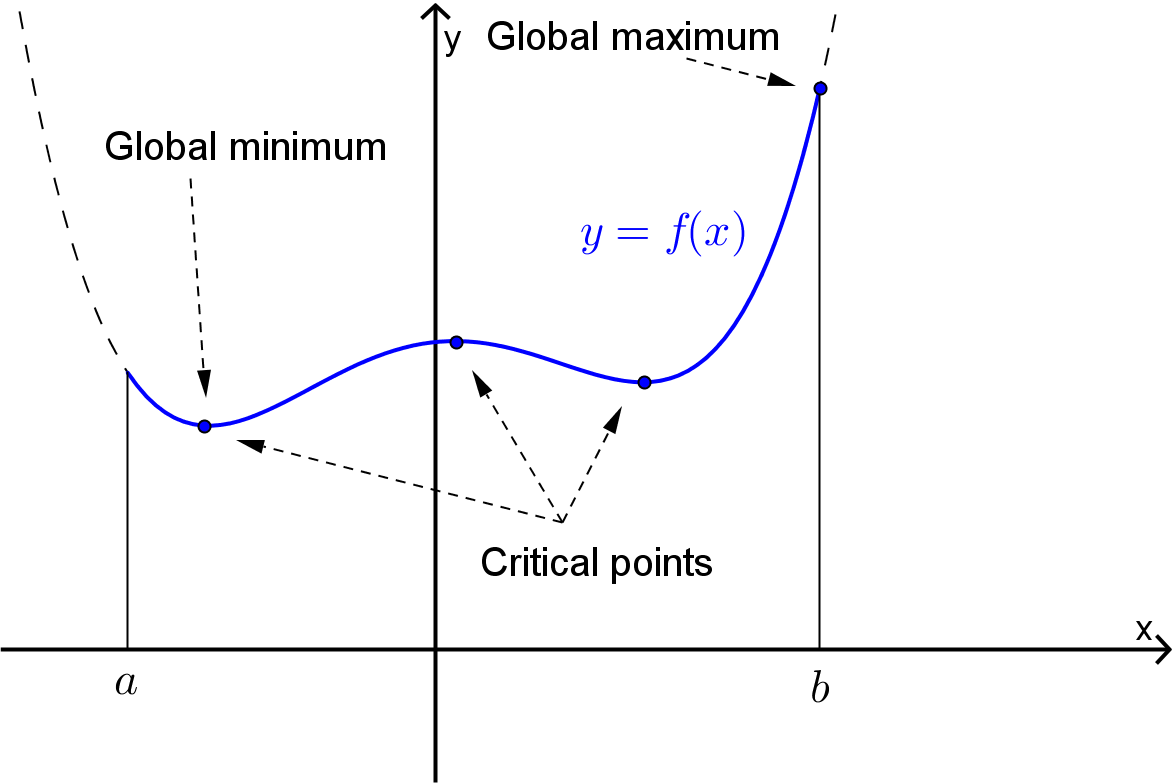
\includegraphics[width=\linewidth]{./Calculus/Images/7/Fig8_Global_Extrema_1D.png}
\end{image}%
\tcblower
\end{figureptx}%
These global extrema can be found by evaluating \(f(x)\) at%
\par
%
\begin{itemize}[label=\textbullet]
\item{}All of the critical points of \(f(x)\) in \(I\), and%
\item{}The endpoints of \(L\).%
\end{itemize}
%
\par
The procedure for finding the global extrema of functions of two variables is very similar and is based on the following theorem.%
\begin{theorem}{Extreme Value Theorem.}{}{g:theorem:id552976}%
If \(f(x,y)\) is a continuous function on the closed and bounded domain \(D \subset \mathbb{R}^2\) then \(f(x,y)\) has both a global maximum and a global minimum on \(D\).%
\end{theorem}
Note that a \emph{closed} region, \(D \subset \mathbb{R}^2\), is a region in the plane that contains its boundary. For example in the diagram below Region \(D_1\) would be a closed region whereas Region \(D_2\) is not closed.%
\begin{figureptx}{}{x:figure:Fig9_closed_region}{}%
\begin{image}{0.275}{0.45}{0.275}%
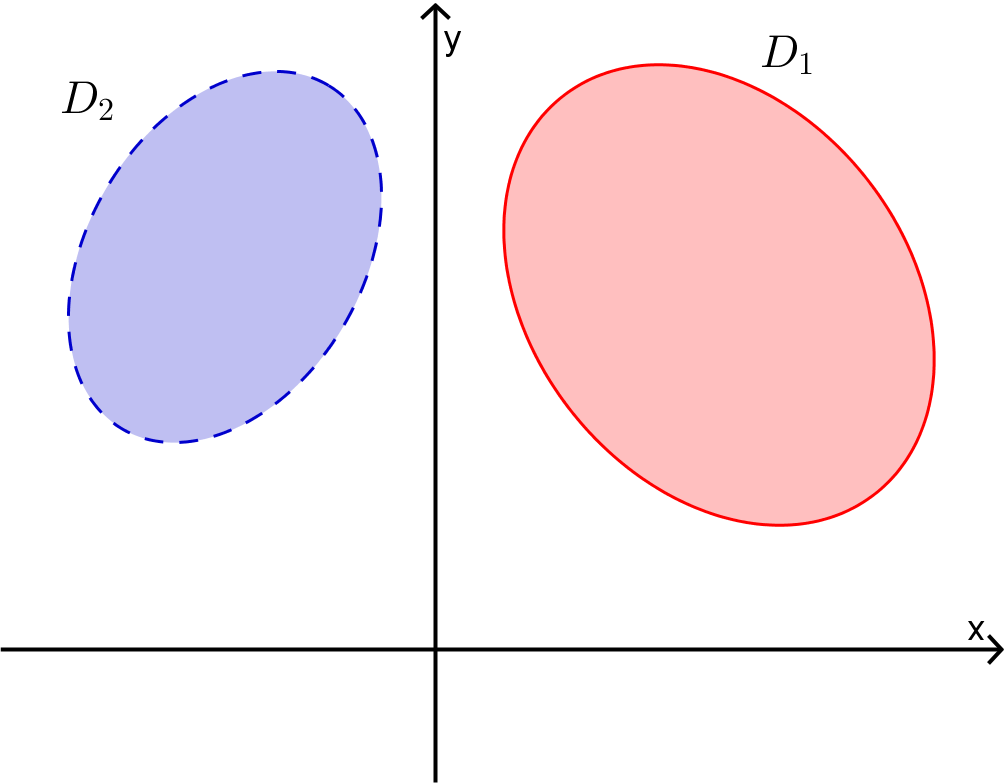
\includegraphics[width=\linewidth]{./Calculus/Images/7/Fig9_closed_region.png}
\end{image}%
\tcblower
\end{figureptx}%
A \emph{bounded} region, \(D \subset \mathbb{R}^2\), is a region in the plane that doesn’t extend to infinity in any direction. For example in the diagram below Region \(D_1\) would be a bounded region whereas Region \(D_2\) is not bounded.%
\begin{figureptx}{}{x:figure:Fig10_bounded_region}{}%
\begin{image}{0.275}{0.45}{0.275}%
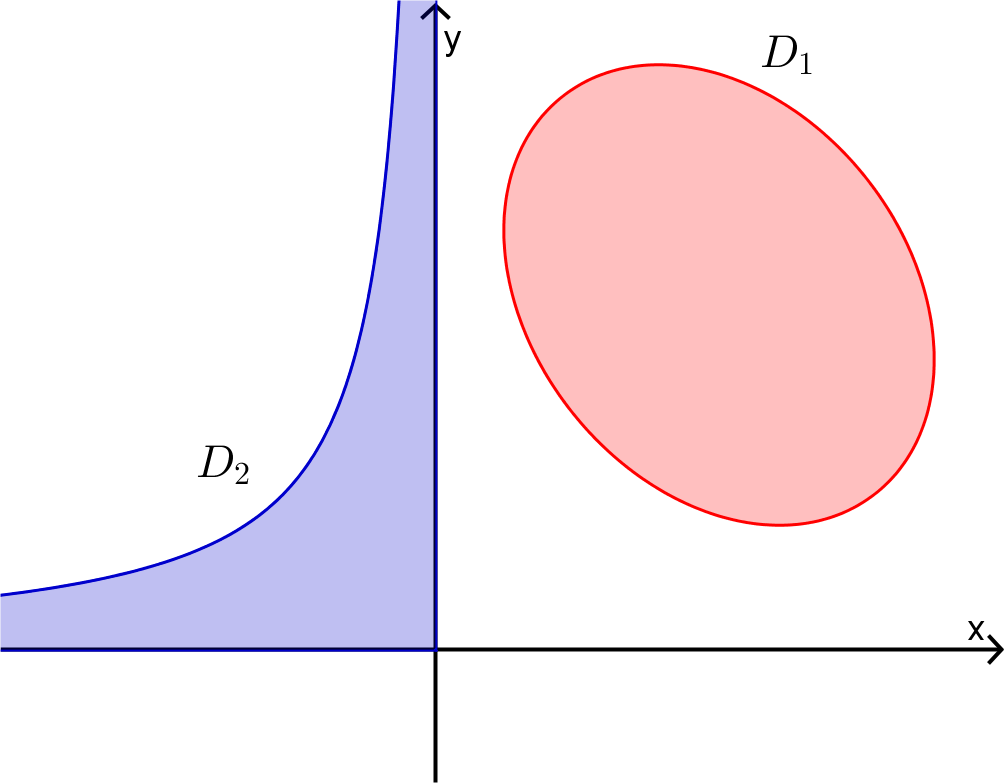
\includegraphics[width=\linewidth]{./Calculus/Images/7/Fig10_bounded_region.png}
\end{image}%
\tcblower
\end{figureptx}%
\begin{remark}{Locating Global Extrema.}{g:remark:id553042}%
To locate the global extrema of the continuous function \(f(x,y)\) on the closed and bounded domain \(D \subset \mathbb{R}^2\):%
\par
%
\begin{itemize}[label=\textbullet]
\item{}Find all of the critical points in the interior of \(D\);%
\item{}Find the maximum and minimum values of \(f(x,y)\) on the boundary of \(D\);%
\item{}Evaluate \(f(x,y)\) at each of the above points and compare.%
\end{itemize}
%
\end{remark}
\begin{example}{}{g:example:id553084}%
Find the global extrema of the function \(z(x,y) = x^2 + 2xy + 3y^2\) on the closed triangular region \(D\) with vertices \((-1,1)\), \((2,1)\) and \((-1,-2)\).%
\par\smallskip%
\noindent\textbf{\blocktitlefont Solution}.\hypertarget{g:solution:id553142}{}\quad{}\begin{figureptx}{}{x:figure:Fig11_Example7}{}%
\begin{image}{0.2}{0.6}{0.2}%
\includegraphics[width=\linewidth]{./Calculus/Images/7/Fig11_Example7.png}
\end{image}%
\tcblower
\end{figureptx}%
Firstly note that \(D\) is a closed and bounded region in the plane and so we can use the method outlined above. So begin by finding the critical points of \(z\). Here%
\begin{equation*}
z_x = 2x+2y \: \text{ and } \: z_y = 2x+6y\text{.}
\end{equation*}
%
\par
Critical points occur when z\textunderscore{}x = z\textunderscore{}y = 0 and so this function has only one critical point at \((x,y) = (0,0)\). This is inside \(D\) and so we evaluate the function at this point, i.e.%
\begin{equation*}
z(0,0) = 0\text{.}
\end{equation*}
%
\par
To find the maximum and minimum values of the function on the boundary we will have to consider the 3 sides of the triangle separately. Firstly, consider the side of the triangle defined by%
\begin{equation*}
y=1, \: -1 \leq x \leq 2\text{.}
\end{equation*}
%
\par
On this interval we think of \(z\) as a function of \(x\) only, i.e.%
\begin{equation*}
z(x) = x^2 + 2x + 3\text{.}
\end{equation*}
%
\begin{figureptx}{}{x:figure:Fig12_Example7_z_function}{}%
\begin{image}{0.2}{0.6}{0.2}%
\includegraphics[width=\linewidth]{./Calculus/Images/7/Fig12_Example7_z_function.png}
\end{image}%
\tcblower
\end{figureptx}%
This has a maximum value \(11\) at \(x=2\) and minimum value \(2\) at \(x=1\).%
\par
Next consider the side of the triangle defined by%
\begin{equation*}
x=-1, \: -2 \leq y \leq 1\text{.}
\end{equation*}
On this interval we think of \(z\) as a function of \(y\) only, i.e.%
\begin{equation*}
z(y) = 1-2y+3y^2\text{.}
\end{equation*}
%
\begin{figureptx}{}{x:figure:Fig13_Example7_z_function_2}{}%
\begin{image}{0.2}{0.6}{0.2}%
\includegraphics[width=\linewidth]{./Calculus/Images/7/Fig13_Example7_z_function_2.png}
\end{image}%
\tcblower
\end{figureptx}%
Again, using the technique given above for locating the global extrema for a function of one variable (or by looking at the graph) we find that the largest value of \(z\) occurs at \(y=-2\) (giving \(z=17\)) and the smallest value of \(z\) occurs at \(y=1/3\), (giving \(z=2/3\)).%
\par
Finally on the interval defined by%
\begin{equation*}
y=x-1, \: -1 \leq x \leq 2\text{,}
\end{equation*}
we can think of \(z\) as a function of \(x\) only, i.e.%
\begin{equation*}
z(x) = 6x^2-8x+3\text{.}
\end{equation*}
%
\begin{figureptx}{}{x:figure:Fig14_Example7_z_function_3}{}%
\begin{image}{0.2}{0.6}{0.2}%
\includegraphics[width=\linewidth]{./Calculus/Images/7/Fig14_Example7_z_function_3.png}
\end{image}%
\tcblower
\end{figureptx}%
For this function the global maximum is \(17\) at \(x=-1\) and the global minimum is \(1/3\) at \(x=2/3\).%
\par
On comparing the value of the function \(z(x,y) = x^2 + 2xy + 3y^2\) at each of the global extrema on the sides of the triangle and at the critical point inside the region we conclude that the function has a global maximum of \(17\) at \((x,y) = (-1,2)\) and a global minimum of \(0\) at \((x,y)=(0,0)\).%
\end{example}
%
%
\typeout{************************************************}
\typeout{Exercises 7.3 Example Tasks}
\typeout{************************************************}
%
\begin{exercises-subsection-numberless}{Example Tasks}{}{Example Tasks}{}{}{g:exercises:id553306}
\begin{divisionexercise}{1}{}{}{g:exercise:id553311}%
Find the global extrema of \(z=2x^2 + x +y^2 - 2\) on \(D = \left \{ (x,y): x^2+y^2 \leq 4 \right \}\).%
\end{divisionexercise}%
\begin{divisionexercise}{2}{}{}{g:exercise:id553312}%
Find the global extrema of \(R(x,y) = x \sqrt{8-x^2-y^2}\) on \(D = \left \{ (x,y): x^2+y^2 \leq 8 \right \}\).%
\end{divisionexercise}%
\end{exercises-subsection-numberless}
\end{sectionptx}
\end{chapterptx}
 %
%
\typeout{************************************************}
\typeout{Chapter 8 Chain Rules}
\typeout{************************************************}
%
\begin{chapterptx}{Chain Rules}{}{Chain Rules}{}{}{x:chapter:Chap-Calculus_8}
%
%
\typeout{************************************************}
\typeout{Section 8.1 The Single Variable Chain Rule}
\typeout{************************************************}
%
\begin{sectionptx}{The Single Variable Chain Rule}{}{The Single Variable Chain Rule}{}{}{x:section:Sec-The_single_variable_chain_rule}
Recall that the chain rule for functions of one variable says:%
\begin{equation*}
\text{If } y=y(x) \text{ and } x=x(t) \text{ then } \dfrac{dy}{dt} = \dfrac{dy}{dx}\cdot \dfrac{dx}{dt}.
\end{equation*}
%
\begin{example}{}{x:example:Ex-Single_variable_chain_rule}%
Use the chain rule to find \(\dfrac{df}{dx}\) if \(f(u) = \sin(u)\) and \(u(x)=x^2+1\).%
\par\smallskip%
\noindent\textbf{\blocktitlefont Answer}.\hypertarget{g:answer:id553425}{}\quad{}\(\dfrac{df}{dx} = 2x\cos(x^2+1)\)%
\par\smallskip%
\noindent\textbf{\blocktitlefont Solution}.\hypertarget{g:solution:id553424}{}\quad{}Via the chain rule:%
\begin{alignat*}{1}
\dfrac{df}{dx} \amp = \dfrac{df}{du}\dfrac{du}{dx}\\
\quad \amp = \cos(u)(2x)\\
\quad \amp = 2x\cos(x^2+1).
\end{alignat*}
%
\end{example}
With multivariable functions there are many ways in which to form composite functions but there will be a chain rule for each possibility. In the following sections we will look at some of these.%
\end{sectionptx}
%
%
\typeout{************************************************}
\typeout{Section 8.2 Multivariable Chain Rules}
\typeout{************************************************}
%
\begin{sectionptx}{Multivariable Chain Rules}{}{Multivariable Chain Rules}{}{}{x:section:Sec-Multivariable-chain-rules}
Begin by considering the case where \(z=z(x,y)\) and \(x=x(t)\), \(y=y(t)\). In this case we can think of \(z\) as defining a real valued function \(z=z(t)\).%
\begin{example}{}{x:example:Ex-Multivariate_chain_rule_substitution}%
If \(z=x^2+2xy+3y^2\) and \(x=t+1\), \(y=t-1\) then find \(z'(t)\) by substituting the expressions for \(x\) and \(y\) into \(z\) and then differentiating.%
\par\smallskip%
\noindent\textbf{\blocktitlefont Answer}.\hypertarget{g:answer:id553530}{}\quad{}\(\dfrac{dz}{dt} = 12t-4\)%
\par\smallskip%
\noindent\textbf{\blocktitlefont Solution}.\hypertarget{g:solution:id553502}{}\quad{}On substituting \(x\) and \(x\) into \(z\)%
\begin{alignat*}{1}
z(t) \amp = (t+1)^2 + 2(t+1)(t-1)+3(t-1)^2\\
\quad \amp = 6t^2-4t+2
\end{alignat*}
Thus%
\begin{equation*}
\dfrac{dz}{dt} = 12-4.
\end{equation*}
%
\end{example}
Now for a function \(f\) of two variables the linear approximation (or '{}'{}small change'{}'{}) formula says:%
\begin{equation*}
\Delta f \approx \dfrac{\partial f}{\partial x}\Delta x + \dfrac{\partial f}{\partial y}\Delta y.
\end{equation*}
Thus%
\begin{equation*}
\dfrac{\Delta f}{\Delta t} \approx \dfrac{\partial f}{\partial x}\frac{\Delta x}{\Delta t} + \dfrac{\partial f}{\partial y}\frac{\Delta y}{\Delta t}.
\end{equation*}
%
\par
This formula becomes more accurate as \(\Delta t \to 0\) and from the limit we obtain the following chain rule.%
\begin{theorem}{Chain Rule 1.}{}{g:theorem:id553553}%
If \(z=z(x,y)\) and \(x=x(t)\), \(y=y(t)\) are differentiable functions then%
\begin{equation*}
\dfrac{dz}{dt} = \dfrac{\partial z}{\partial x}\cdot \dfrac{dx}{dt} + \dfrac{\partial z}{\partial y}\cdot \dfrac{dy}{dt}.
\end{equation*}
%
\end{theorem}
\begin{example}{}{x:example:Ex-Chain_rule_1_sample_1}%
If \(z=x^2+2xy+3y^2\) and \(x=t+1\), \(y=t-1\) then find \(z'(t)\) by using the chain rule.%
\par\smallskip%
\noindent\textbf{\blocktitlefont Answer}.\hypertarget{g:answer:id553601}{}\quad{}\(\dfrac{dz}{dt} = 12t-4\)%
\par\smallskip%
\noindent\textbf{\blocktitlefont Solution}.\hypertarget{g:solution:id553605}{}\quad{}Here%
\begin{equation*}
\dfrac{\partial z}{\partial x} = 2x + 2y, \ \dfrac{\partial z}{\partial y} = 2x + 6y, \ \dfrac{dx}{dt} = 1 = \dfrac{dy}{dt}.
\end{equation*}
So, via the chain rule%
\begin{alignat*}{1}
\dfrac{dz}{dt} \amp = (2x+2y)\times 1 + (2x+6y)\times 1\\
\quad \amp = 4x+8y\\
\quad \amp = 4(t+1)+8(t-1)\\
\quad \amp = 12t-4.
\end{alignat*}
%
\end{example}
\begin{example}{}{x:example:Ex-Chain_rule_1_sample_2}%
Use the chain rule to find \(z'(t)\) when \(z(x,y) = \sqrt{x^2+y^2}\) and \(x(t) = e^{2t}, \ y(t)=e^{-2t}\).%
\par\smallskip%
\noindent\textbf{\blocktitlefont Answer}.\hypertarget{g:answer:id553610}{}\quad{}\(\dfrac{dz}{dt} = \dfrac{2(e^{6t} - e^{-2t})}{\sqrt{e^{8t}+1}}\)%
\par\smallskip%
\noindent\textbf{\blocktitlefont Solution}.\hypertarget{g:solution:id553625}{}\quad{}Here%
\begin{equation*}
\dfrac{\partial z}{\partial x} = \dfrac{x}{\sqrt{x^2+y^2}}, \ \dfrac{\partial z}{\partial y} = \dfrac{y}{\sqrt{x^2+y^2}}, \ \dfrac{dx}{dt} = 2e^{2t}, \ \dfrac{dy}{dt} = -2e^{-2t}.
\end{equation*}
So, via the chain rule%
\begin{alignat*}{1}
\dfrac{dz}{dt} \amp = \dfrac{x}{\sqrt{x^2+y^2}}\times 2e^{2t} + \dfrac{y}{\sqrt{x^2+y^2}}\times (-2e^{-2t})\\
\quad \amp = \dfrac{e^{2t}2e^{2t}}{\sqrt{e^{4t} + e^{-4t}}} -\dfrac{e^{-2t}2e^{-2t}}{\sqrt{e^{4t} + e^{-4t}}}\\
\quad \amp = \dfrac{2(e^{6t} - e^{-2t})}{\sqrt{e^{8t}+1}}.
\end{alignat*}
%
\end{example}
\begin{example}{}{x:example:Ex-Related_rate_chain_rule_1}%
The radius of a right circular cone is increasing at a rate of \(1.8\) cm\slash{}s while its height is decreasing at a rate of \(2.5\) cm\slash{}s. At what rate is the volume of the cone changing when the radius is \(120\) cm and the height is \(140\) cm?%
\par\smallskip%
\noindent\textbf{\blocktitlefont Answer}.\hypertarget{g:answer:id553656}{}\quad{}\(\dfrac{dV}{dt} = 8160\pi \  (\text{cm}^3\text{/s})\)%
\par\smallskip%
\noindent\textbf{\blocktitlefont Solution}.\hypertarget{g:solution:id553702}{}\quad{}The volume \(V\) of right circular cone of radius \(r\) and height \(h\) is%
\begin{equation*}
V(r,h) = \dfrac{1}{3}\pi r^2h.
\end{equation*}
%
\par
Since both radius and the height are functions of time \(t\), i.e. \(r=r(t)\) and \(h=h(t)\), we can think of the volume as a function of time as well, i.e. \(V=V(t)\), and the problem is asking us to find \(\dfrac{dV}{dt}\) when \(r=120\) and \(h=140\). Now, by the chain rule:%
\begin{equation*}
\dfrac{dV}{dt} = \dfrac{\partial V}{\partial r}\cdot \dfrac{dr}{dt} + \dfrac{\partial V}{\partial h}\cdot \dfrac{dh}{dt}.
\end{equation*}
%
\par
Here%
\begin{equation*}
\dfrac{\partial V}{\partial r}  = \dfrac{2}{3}\pi rh \text{ and } \dfrac{\partial V}{\partial h} =\dfrac{1}{3}\pi r^2
\end{equation*}
and we are given that \(\dfrac{dr}{dt} = 1.8\) and \(\dfrac{dh}{dt} = -2.5\). (Note that \(\dfrac{dh}{dt}\) is negative because the height is decreasing.) Thus, at \(r=120\) and \(h=140\)%
\begin{alignat*}{1}
\dfrac{dV}{dt} \amp = \dfrac{2\pi}{3} \times 120 \times 140 \times 1.8  - \dfrac{\pi}{3}\times 120^2 \times 2.5\\
\amp =  8160\pi \  (\text{cm}^3\text{/s})
\end{alignat*}
%
\end{example}
Consider the case now where \(z=z(u)\) and \(u=u(x,y)\). In this case we can think of \(z\) as defining a function of two variables \(z=z(x,y)\) and hence has partial derivatives with respect to these variables. The relevant chain rules for this case are:%
\begin{theorem}{Chain Rule 2.}{}{g:theorem:id553776}%
If \(z=z(u)\) and \(u=u(x,y)\) are differentiable functions then%
\begin{equation*}
\dfrac{\partial z}{\partial x} =  \dfrac{dz}{du}\cdot\dfrac{\partial u}{\partial x} \quad \text{and} \quad  \dfrac{\partial z}{\partial y} = \dfrac{dz}{du}\cdot\dfrac{\partial u}{\partial y}.
\end{equation*}
%
\end{theorem}
\begin{example}{}{x:example:Ex-Related_rate_chain_rule_2}%
A spherical balloon holds a fixed amount of gas but its volume is dependent on the pressure \(P\) and temperature \(T\) of the gas according to%
\begin{equation*}
V=k\dfrac{T}{P}, \quad k \ \text{ a constant}.
\end{equation*}
Determine expressions for the rate of change of the radius \(r\) of the balloon with respect to the pressure and temperature of the gas.%
\par\smallskip%
\noindent\textbf{\blocktitlefont Answer}.\hypertarget{g:answer:id553827}{}\quad{}\(\dfrac{\partial r}{\partial P} = -\dfrac{1}{3}Ck^{\frac{1}{3}}T^{\frac{1}{3}}P^{-\frac{4}{3}}\)%
\par
\(\dfrac{\partial r}{\partial T} =  \dfrac{1}{3}Ck^{\frac{1}{3}}T^{-\frac{2}{3}}P^{-\frac{1}{3}}\)%
\par\smallskip%
\noindent\textbf{\blocktitlefont Solution}.\hypertarget{g:solution:id553838}{}\quad{}The volume \(V\) of a sphere of radius \(r\) is%
\begin{equation*}
V = \dfrac{4}{3}\pi r^3.
\end{equation*}
%
\par
Thus we can think of the radius of the balloon as a function of its volume, i.e.%
\begin{equation*}
r(V) = CV^{\frac{1}{3}} \text{ where } C=\left(\dfrac{3}{4\pi}\right)^{\frac{1}{3}}
\end{equation*}
where the volume is, in turn, a function of the pressure and temperature of the gas, i.e.%
\begin{equation*}
V(P,T) = kP^{-1}T.
\end{equation*}
%
\par
Using Chain Rule 2:%
\begin{alignat*}{1}
\dfrac{\partial r}{\partial P} \amp = \dfrac{dr}{dV}\dfrac{\partial V}{\partial P}\\
\amp =  \left(\dfrac{1}{3}CV^{-\frac{2}{3}}\right)(-kTP^{-2})\\
\amp = -\dfrac{1}{3}Ck^{\frac{1}{3}}T^{\frac{1}{3}}P^{-\frac{4}{3}}.
\end{alignat*}
%
\par
Similarly%
\begin{alignat*}{1}
\dfrac{\partial r}{\partial T} \amp = \dfrac{dr}{dV}\dfrac{\partial V}{\partial T}\\
\amp =  \left(\dfrac{1}{3}CV^{-\frac{2}{3}}\right)(kP^{-1})\\
\amp =  \dfrac{1}{3}Ck^{\frac{1}{3}}T^{-\frac{2}{3}}P^{-\frac{1}{3}}.
\end{alignat*}
%
\end{example}
\begin{example}{}{x:example:Ex-Chain_rule_2_sample}%
Use the appropriate chain rules to calculate \(\dfrac{\partial z}{\partial x}\) and \(\dfrac{\partial z}{\partial y}\) when%
\begin{equation*}
z = \dfrac{u}{u+1} \text{ and } u = 3x^5-5xy^2.
\end{equation*}
%
\par\smallskip%
\noindent\textbf{\blocktitlefont Answer}.\hypertarget{g:answer:id553896}{}\quad{}\(\dfrac{\partial z}{\partial x} = \dfrac{15x^4-5y^2}{(3x^5-5xy^2+1)^2}\)%
\par
\(\dfrac{\partial z}{\partial y} = \dfrac{-10xy}{(3x^5-5xy^2+1)^2}\)%
\par\smallskip%
\noindent\textbf{\blocktitlefont Solution}.\hypertarget{g:solution:id553905}{}\quad{}Using Chain Rule 2:%
\begin{equation*}
\dfrac{\partial z}{\partial x} =  \dfrac{dz}{du}\dfrac{\partial u}{\partial x} \text{ and } \dfrac{\partial z}{\partial y} = \dfrac{dz}{du}\dfrac{\partial u}{\partial y}.
\end{equation*}
%
\par
Now, (via the quotient rule)%
\begin{equation*}
\dfrac{dz}{du} = \dfrac{(u+1)(1) - u(1)}{(u+1)^2} = \dfrac{1}{(u+1)^2}
\end{equation*}
and%
\begin{equation*}
\dfrac{\partial u}{\partial x} = 15x^4-5y^2 \text{ and } \dfrac{\partial u}{\partial y} = -10xy.
\end{equation*}
%
\par
Thus%
\begin{equation*}
\dfrac{\partial z}{\partial x} = \dfrac{15x^4-5y^2}{(3x^5-5xy^2+1)^2} \text{ and } \dfrac{\partial z}{\partial y} = \dfrac{-10xy}{(3x^5-5xy^2+1)^2}.
\end{equation*}
%
\end{example}
Next consider the case where \(z=z(x,y)\) and \(x=x(s,t)\), \(y=y(s,t)\). In this case we can think of \(z\) as defining a function of two variables \(z=z(s,t)\). The relevant chain rules for this case are:%
\begin{theorem}{Chain Rule 3.}{}{g:theorem:id553925}%
If \(z=z(x,y)\) and \(x=x(s,t)\), \(y=y(s,t)\) are differentiable functions then%
\begin{equation*}
\dfrac{\partial z}{\partial s} = \dfrac{\partial z}{\partial x} \cdot \dfrac{\partial x}{\partial s} + \dfrac{\partial z}{\partial y} \cdot \dfrac{\partial y}{\partial s}
\end{equation*}
%
\begin{equation*}
\dfrac{\partial z}{\partial t} = \dfrac{\partial z}{\partial x} \cdot \dfrac{\partial x}{\partial t} + \dfrac{\partial z}{\partial y} \cdot \dfrac{\partial y}{\partial t}
\end{equation*}
%
\end{theorem}
\begin{example}{}{x:example:Ex-Chain_rule_3_sample}%
Use the appropriate chain rules to find \(\dfrac{\partial z}{\partial s}\) and \(\dfrac{\partial z}{\partial t}\) when%
\begin{equation*}
z = \dfrac{x}{y} \text{ and } x = se^t, \quad y = 1+se^{-t}.
\end{equation*}
%
\par\smallskip%
\noindent\textbf{\blocktitlefont Answer}.\hypertarget{g:answer:id553972}{}\quad{}\(\dfrac{\partial z}{\partial s} = \dfrac{e^t}{(1+se^{-t})^2}\)%
\par
\(\dfrac{\partial z}{\partial y} = \dfrac{se^t+2s^2}{(1+se^{-t})^2}\)%
\par\smallskip%
\noindent\textbf{\blocktitlefont Solution}.\hypertarget{g:solution:id554030}{}\quad{}Here%
\begin{equation*}
\dfrac{\partial z}{\partial x} = \dfrac{1}{y}, \quad \dfrac{\partial z}{\partial y} = -\dfrac{x}{y^2}
\end{equation*}
and%
\begin{equation*}
\dfrac{\partial x}{\partial s} = e^t, \quad \dfrac{\partial x}{\partial t} = se^t, \quad \dfrac{\partial y}{\partial s}=e^{-t}, \quad \dfrac{\partial y}{\partial t}=-se^{-t}.
\end{equation*}
%
\par
Thus, by Chain Rule 3%
\begin{alignat*}{1}
\dfrac{\partial z}{\partial s} \amp = \dfrac{\partial z}{\partial x} \cdot \dfrac{\partial x}{\partial s} + \dfrac{\partial z}{\partial y} \cdot \dfrac{\partial y}{\partial s}\\
\amp =  \left(\dfrac{1}{1+se^{-t}}\right)(e^t) + \left(\dfrac{-se^t}{(1+se^{-t})^2}\right)(e^{-t})\\
\amp =  \dfrac{e^t}{(1+se^{-t})^2}
\end{alignat*}
and%
\begin{alignat*}{1}
\dfrac{\partial z}{\partial t} \amp = \dfrac{\partial z}{\partial x} \cdot \dfrac{\partial x}{\partial t} + \dfrac{\partial z}{\partial y} \cdot \dfrac{\partial y}{\partial t}\\
\amp =  \left(\dfrac{1}{1+se^{-t}}\right)(se^t) + \left(\dfrac{-se^t}{(1+se^{-t})^2}\right)(-se^{-t})\\
\amp =  \dfrac{se^t + 2s^2}{(1+se^{-t})^2}
\end{alignat*}
%
\end{example}
The chain rules given above are just special cases of the general chain rule.%
\begin{theorem}{The General Chain Rule.}{}{g:theorem:id554042}%
If \(z=z(x_1,x_2,\ldots,x_n)\) is a differentiable function of \(n\) variables \(x_1,x_2,\ldots,x_n\) and each \(x_i = x_i(t_1,t_2,\ldots,t_m)\) is a differentiable function of the \(m\) variables \(t_1,t_2,\ldots,t_m\) then%
\begin{equation*}
\dfrac{\partial z}{\partial t_i} = \dfrac{\partial z}{\partial x_1} \cdot \dfrac{\partial x_1}{\partial t_i} + \dfrac{\partial z}{\partial x_2} \cdot \dfrac{\partial x_2}{\partial t_i} + \cdots + \dfrac{\partial z}{\partial x_n} \cdot \dfrac{\partial x_n}{\partial t_i}
\end{equation*}
for each \(i = 1,2,\ldots, m.\)%
\end{theorem}
\begin{example}{}{x:example:Ex-General_chain_rule_sample}%
Find \(\dfrac{\partial w}{\partial u}\) if \(w(x,y,z) = 2x^2+5y^2+z^3\) and%
\begin{equation*}
x(r,s,t,u) = r+s+t+u, \quad y(r,s,t,u)=r^2,\quad z(r,s,t,u) = \sqrt{r-s+t-u}
\end{equation*}
%
\par\smallskip%
\noindent\textbf{\blocktitlefont Answer}.\hypertarget{g:answer:id551826}{}\quad{}\(\dfrac{\partial w}{\partial u} = 4(r+s+t+u) - \dfrac{3\sqrt{r-s+t-u}}{2}\)%
\par\smallskip%
\noindent\textbf{\blocktitlefont Solution}.\hypertarget{g:solution:id551842}{}\quad{}By the general Chain Rule%
\begin{alignat*}{1}
\dfrac{\partial w}{\partial u} \amp = \dfrac{\partial w}{\partial x}\dfrac{\partial x}{\partial u} + \dfrac{\partial w}{\partial y}\dfrac{\partial y}{\partial u} + \dfrac{\partial w}{\partial z}\dfrac{\partial z}{\partial u}\\
\amp =  (4x)(1) + (10y)(0) + (3z^2)\left(\dfrac{1}{2}(r-s+t-u)^{-\frac{1}{2}}(-1)\right)\\
\amp =  4(r+s+t+u) - \dfrac{3\sqrt{r-s+t-u}}{2}
\end{alignat*}
%
\end{example}
%
%
\typeout{************************************************}
\typeout{Exercises 8.2 Example Tasks}
\typeout{************************************************}
%
\begin{exercises-subsection-numberless}{Example Tasks}{}{Example Tasks}{}{}{g:exercises:id551862}
\begin{divisionexercise}{1}{}{}{g:exercise:id551866}%
Use the appropriate chain rules to find \(\dfrac{\partial z}{\partial x}\) and \(\dfrac{\partial z}{\partial y}\) when%
\begin{equation*}
z(u,v)=u^2v+e^v  \quad \text{and} \quad u(x,y) = \ln(y-x), \quad v(x,y) = x+xy.
\end{equation*}
\end{divisionexercise}%
\begin{divisionexercise}{2}{}{}{g:exercise:id551844}%
Two straight roads intersect at right angles. Car A is moving on one road approaches the intersection at \(25\) km\slash{}h while Car B moving on the other road approaches the intersection at \(30\) km\slash{}h. At what rate is the distance between the cars changing when A is \(0.3\) km from the intersection and B is \(0.4\) km from the intersection?\end{divisionexercise}%
\begin{divisionexercise}{3}{}{}{g:exercise:id551912}%
Show that any function of the form%
\begin{equation*}
z = f(x+at) + g(x-at)
\end{equation*}
is a solution of the wave equation%
\begin{equation*}
\dfrac{\partial^2 z}{\partial t^2} = a^2\dfrac{\partial^2 z}{\partial x^2}.
\end{equation*}
\end{divisionexercise}%
\begin{divisionexercise}{4}{}{}{g:exercise:id551885}%
%
\begin{enumerate}[label=\alph*]
\item{}If \(z=z(x,y)\) and \(x=x(\theta)\) and \(y=y(\theta)\) find an appropriate chain rule for \(\dfrac{d^2z}{d\theta^2}\).%
\item{}Using the result of part (a) find \(\dfrac{d^2z}{d\theta^2}\) when \(z(x,y)=x^2+2y\) and \(x(\theta) = 5\cos(\theta)\) and \(y(\theta) = 5\sin(\theta)\).%
\end{enumerate}
\end{divisionexercise}%
\end{exercises-subsection-numberless}
\end{sectionptx}
%
%
\typeout{************************************************}
\typeout{Section 8.3 Implicit Differentiation}
\typeout{************************************************}
%
\begin{sectionptx}{Implicit Differentiation}{}{Implicit Differentiation}{}{}{g:section:id554781}
We can use our chain rules to produce another way looking at implicit differentiation. Assuming that the equation%
\begin{equation*}
F(x,y) = 0
\end{equation*}
implicitly defines the function \(y=y(x)\), recall that implicit differentiation gives us a way of finding a formula for  \(\dfrac{dy}{dx}\).%
\begin{example}{}{x:example:Ex-Implicit_differentiation_recall}%
Use implicit differentiation to find a formula for \(\dfrac{dy}{dx}\) for the function \(y=y(x)\) implicitly defined by the equation%
\begin{equation*}
x\cos(y) + y\cos(x) =x\text{.}
\end{equation*}
%
\par\smallskip%
\noindent\textbf{\blocktitlefont Answer}.\hypertarget{g:answer:id554823}{}\quad{}\(\dfrac{dy}{dx} = \dfrac{1-\cos(y)+y\sin(x)}{\cos(x)-x\sin(y)}\)%
\par\smallskip%
\noindent\textbf{\blocktitlefont Solution}.\hypertarget{g:solution:id554790}{}\quad{}Differentiating both sides of the equation with respect to \(x\)%
\begin{alignat*}{1}
\dfrac{d}{dx}\left(x\cos(y) + y\cos(x)\right) \amp = \dfrac{d}{dx}(x)\\
\left(-x\sin(y)\dfrac{dy}{dx} + \cos(y)\right) + \left(-y\sin(x)+\cos(x)\dfrac{dy}{dx}\right) \amp =  1\\
\dfrac{dy}{dx}\left(\cos(x)-x\sin(y)\right) \amp = 1-\cos(y) +y\sin(x)\\
\dfrac{dy}{dx} \amp = \dfrac{1-\cos(y)+y\sin(x)}{\cos(x)-x\sin(y)}
\end{alignat*}
%
\end{example}
To use the chain rules to find a formula for \(\dfrac{dy}{dx}\) for the function implicitly defined by the equation%
\begin{equation}
F(x,y)=0\label{x:men:Eqn-Implicit_function}
\end{equation}
let%
\begin{equation*}
z=F(x,y) \text{ and }  x=x(t), \quad y=y(t).
\end{equation*}
Thus we can think of \(F\) as being a function of the one variable \(t\), and so, by Chain Rule 1,%
\begin{equation*}
\dfrac{dz}{dt} = \dfrac{\partial F}{\partial x}\dfrac{dx}{dt} + \dfrac{\partial F}{\partial y}\dfrac{dy}{dt}.
\end{equation*}
Now we are thinking of equation \hyperref[x:men:Eqn-Implicit_function]{({\xreffont\ref{x:men:Eqn-Implicit_function}})} as defining a function of one variable \(y=y(x)\), so let \(x=t\) and \(y=y(t)\) and hence%
\begin{equation}
\dfrac{dz}{dt} = \dfrac{\partial F}{\partial x}\times (1) + \dfrac{\partial F}{\partial y}\dfrac{dy}{dt} = F_x + F_y \dfrac{dy}{dt}.\label{g:men:id554890}
\end{equation}
%
\par
Returning to equation \hyperref[x:men:Eqn-Implicit_function]{({\xreffont\ref{x:men:Eqn-Implicit_function}})}, on differentiating both sides with respect to \(t\), we obtain%
\begin{alignat*}{1}
\dfrac{dz}{dt} \amp= \dfrac{d}{dt}(0)\\
F_x + F_y \dfrac{dy}{dt} \amp = 0.
\end{alignat*}
Of course \(x=t\) so \(\dfrac{dy}{dx} = \dfrac{dy}{dt}\) from which we obtain, provided \(F_y \neq 0\),%
\begin{equation*}
\dfrac{dy}{dx} = -\dfrac{F_x}{F_y}.
\end{equation*}
%
\par
Thus we can find a formula for \(\dfrac{dy}{dx}\) via partial differentiation as opposed to implicit differentiation. In summary:%
\begin{theorem}{}{}{g:theorem:id554907}%
If the equation \(F(x,y) = 0\) implicitly defines the function \(y=y(x)\) then%
\begin{equation*}
\dfrac{dy}{dx} = -\dfrac{F_x}{F_y}  \text{ provided } F_y \neq 0.\
\end{equation*}
%
\end{theorem}
\begin{example}{}{x:example:Ex-Implicit_differentiation_via_partial_differentiation}%
Use partial differentiation to find a formula for \(\dfrac{dy}{dx}\) for the function \(y=y(x)\) implicitly defined by the equation%
\begin{equation*}
x\cos(y) + y\cos(x) =x\text{.}
\end{equation*}
%
\par\smallskip%
\noindent\textbf{\blocktitlefont Answer}.\hypertarget{g:answer:id554941}{}\quad{}\(\dfrac{dy}{dx} = \dfrac{1-\cos(y)+y\sin(x)}{\cos(x)-x\sin(y)}\)%
\par\smallskip%
\noindent\textbf{\blocktitlefont Solution}.\hypertarget{g:solution:id554965}{}\quad{}Let%
\begin{equation*}
F(x,y) = x\cos(y) + y\cos(x) - x\text{.}
\end{equation*}
Then%
\begin{equation*}
\dfrac{\partial F}{\partial x} = \cos(y)-y\sin(x)-1 \text{ and } \dfrac{\partial F}{\partial y} = -x\sin(y)+\cos(x).
\end{equation*}
Thus%
\begin{alignat*}{1}
\dfrac{dy}{dx} \amp = -\dfrac{F_x}{F_y}\\
\amp = \dfrac{1-\cos(y)+y\sin(x)}{\cos(x)-x\sin(y)}.
\end{alignat*}
%
\end{example}
A similar argument can extend this result to functions of more than one variable. For example:%
\begin{theorem}{}{}{g:theorem:id554974}%
If \(F(x,y,z) = 0\) implicitly defines the function \(z=f(x,y)\) then%
\begin{equation*}
\dfrac{\partial z}{\partial x} = -\dfrac{F_x}{F_z} \text{ and } \dfrac{\partial z}{\partial y} = -\dfrac{F_y}{F_z}, \text{ provided } F_z \neq 0. \
\end{equation*}
%
\end{theorem}
\begin{example}{}{x:example:Ex-Implicit_differentiation_via_partial_differentiation_general}%
Use partial differentiation to find formulas for \(\dfrac{\partial z}{\partial s} \text{ and } \dfrac{\partial z}{\partial t}\) for the function \(z=z(s,t)\) implicitly defined by the equation%
\begin{equation*}
z^2 +\cos(s) + \ln(st) = 3.
\end{equation*}
%
\par\smallskip%
\noindent\textbf{\blocktitlefont Answer}.\hypertarget{g:answer:id554985}{}\quad{}\(\dfrac{\partial z}{\partial s} = \dfrac{\sin(s)-\frac{1}{s}}{2z}\)%
\par
\(\dfrac{\partial z}{\partial t} = -\dfrac{1}{2zt}\)%
\par\smallskip%
\noindent\textbf{\blocktitlefont Solution}.\hypertarget{g:solution:id555034}{}\quad{}Let%
\begin{equation*}
F(s,t,z) = z^2 + \cos(s) + \ln(st)-3\text{.}
\end{equation*}
Then%
\begin{equation*}
F_s = -\sin(s)+\dfrac{1}{s}, \quad F_t=\dfrac{1}{t}, F_z=2z.
\end{equation*}
Thus%
\begin{equation*}
\dfrac{\partial z}{\partial s} = -\dfrac{F_s}{F_z} = \dfrac{\sin(s)-\frac{1}{s}}{2z}
\end{equation*}
%
\begin{equation*}
\dfrac{\partial z}{\partial t} = -\dfrac{F_t}{F_z}=-\dfrac{1}{2zt}.
\end{equation*}
%
\end{example}
%
%
\typeout{************************************************}
\typeout{Exercises 8.3 Example Tasks}
\typeout{************************************************}
%
\begin{exercises-subsection-numberless}{Example Tasks}{}{Example Tasks}{}{}{g:exercises:id555025}
\begin{divisionexercise}{1}{}{}{g:exercise:id555029}%
Using partial differentiation (as opposed to implicit differentiation) find \(\dfrac{\partial z}{\partial x}\) at \((x,y,z) = (1,2,1)\) when the function \(z(x,y)\) is defined by the equation%
\begin{equation*}
(x-y)e^z + (y-z)e^x + (z-x)e^y = 0.
\end{equation*}
\end{divisionexercise}%
\end{exercises-subsection-numberless}
\end{sectionptx}
\end{chapterptx}
\end{partptx}
%
%
\typeout{************************************************}
\typeout{Part II Differential Equations}
\typeout{************************************************}
%
\begin{partptx}{Differential Equations}{}{Differential Equations}{}{}{x:part:Part-Differenial_Equations}
 %
%
\typeout{************************************************}
\typeout{Chapter 9 Introduction}
\typeout{************************************************}
%
\begin{chapterptx}{Introduction}{}{Introduction}{}{}{x:chapter:Differential_Equations_1}
%
%
\typeout{************************************************}
\typeout{Section 9.1 Introduction}
\typeout{************************************************}
%
\begin{sectionptx}{Introduction}{}{Introduction}{}{}{x:section:introduction}
Most of the equations that we have come across so far in our mathematical "upbringing" have imposed conditions that a \terminology{number} is required to satisfy.%
\begin{example}{}{g:example:id555113}%
Let \(x\) be a real number. Solve%
\begin{equation*}
x^3-x^2-2x+2=0 
\end{equation*}
%
\par\smallskip%
\noindent\hypertarget{g:solution:id555150}{}By factoring the left hand side we obtain%
\par
%
\begin{align*}
x^2(x-1)-2(x-1) \amp =0\\
(x^2-2)(x-1)\amp =0\\
x \amp =1,\sqrt{2},-\sqrt{2}
\end{align*}
%
\par
Thus we have found the numbers that satisfy the conditions imposed by the equation. Notice that we can check our answers by substituting back into the original equation. For example, when \(x=1\),%
\begin{equation*}
LHS=(1)^3-(1)^2-2(1)+2=0=RHS
\end{equation*}
By way of terminology, we would say that \(x=1\) is \terminology{a} solution to the equation whereas the set of \terminology{all} solutions is \(x=1,\sqrt{2},-\sqrt{2}\). An equivalent terminology (which we will use subsequently) is \(x=1\) is a \terminology{particular solution} whereas \(x=1,\sqrt{2},-\sqrt{2}\) is the \terminology{general solution} for this equation.%
\end{example}
\begin{example}{}{g:example:id555198}%
Let \(x\) be a real number. Solve%
\begin{equation*}
x=\tan(x) 
\end{equation*}
%
\par\smallskip%
\noindent\hypertarget{g:solution:id555205}{}The strategy that we used for solving the equation in Example 1 won’t work for this equation. In fact we cannot write down the solution (or solutions) to this equation in closed form. Thus we adopt the strategy of finding an approximation to the solutions.%
\par
We could do this geometrically by plotting the graphs of \(y=x\) and \(y=\tan(x)\) and looking at the points of intersection. \begin{figureptx}{}{g:figure:id555217}{}%
\begin{image}{0.125}{0.75}{0.125}%
\includegraphics[width=\linewidth]{./DifferentialEquations/Images/1/1_example2.png}
\end{image}%
\tcblower
\end{figureptx}%
 As can be seen in Figure 9.1.3., there will be an infinite number of solutions to this equation. One solution is \(x=0\). There is another solution between \(x=4\) and \(x=5\) and so on.%
\par
Another way of approximating the solution would be numerically. We could use Newton’s method for example. Starting with an initial guess of \(x_0=4.5\) our next guess is%
\begin{equation*}
x_1=x_0-\frac{f(x_0)}{f'(x_0)}=4.5-\frac{\tan(4.5)-4.5}{\sec^2(4.5)-1}=4.4936 \textrm{ (to 4 d.p.)}\text{,}
\end{equation*}
and so on.%
\end{example}
Mathematical models in science and engineering often throw up a situation where information about a function's derivative (or derivatives) is known. From here, we usually want to deduce information about the function itself.%
\begin{example}{}{g:example:id555241}%
It has been observed that an object cools at a rate proportional to the difference between the object's temperature and ambient temperature. Write down an equation that conveys this observation.%
\par\smallskip%
\noindent\hypertarget{g:solution:id555219}{}Let \(T(t)\) be the temperature of the object at time \(t\) after we begin the observation. Also let \(T_a\) be the ambient temperature. Then%
\begin{equation*}
\frac{dT}{dt}=-k(T-T_a)
\end{equation*}
where \(k\) is a constant.%
\end{example}
As illustrated in Example 9.1.4., we were able to write the \terminology{information} known about the situation in terms of an equation involving the function and the derivative of the function even though we didn’t know what the actual function was. Such an equation is called a \terminology{differential equation} (DE). Having determined the differential equation, we now want to find a \terminology{function} that satisfies the equation, i.e. we want to find a solution to the DE.%
\begin{example}{Example 9.1.4. (cont.).}{g:example:id555253}%
Assuming that the ambient temperature is fixed, what can we say happens to the temperature of the body over time?%
\par\smallskip%
\noindent\hypertarget{g:solution:id555291}{}Solutions to the DE for the temperature of the cooling body are of the form%
\begin{equation*}
T(t)=Ae^{-kt}+T_a 
\end{equation*}
where \(A\) is an arbitrary constant. Even though we haven’t yet looked at the method for finding this solution we can check that it is correct by substituting back into the original equation. Here%
\begin{equation*}
LHS=\frac{dT}{dt}=\frac{d}{dt}\left(Ae^{-kt}+T_a \right)=-kAe^{-kt} 
\end{equation*}
and%
\begin{equation*}
RHS=-k(T-T_a)=-k(Ae^{-kt}+T_a-T_a)=-kAe^{-kt}
\end{equation*}
Once we know the function itself we can now answer questions concerning the temperature of the cooling body over time. For example we see that over time, the temperature of the body starts out at \(A+T_a\) and falls exponentially toward \(T_a\). See Figure 9.1.6. \begin{figureptx}{}{g:figure:id555286}{}%
\begin{image}{0.125}{0.75}{0.125}%
\includegraphics[width=\linewidth]{./DifferentialEquations/Images/1/1_example3.png}
\end{image}%
\tcblower
\end{figureptx}%
%
\end{example}
\begin{example}{}{g:example:id555297}%
A population of bacteria reproduces at a rate proportional to the population. If the population of bacteria is \(N_0\) at the beginning of the study, predict the behaviour of this population over time.%
\par\smallskip%
\noindent\hypertarget{g:solution:id555342}{}Let \(N(t)\) be the number of bacteria present at time \(t\) after the study begins. Then%
\begin{equation*}
\frac{dN}{dt}=kN 
\end{equation*}
where \(k\) is some positive constant. Thus, even though we don’t know what the actual function, \(N(t)\), is we have written a differential equation that the function must satisfy. Note that we also know that the function must satisfy \(N(0)=N_0\).%
\end{example}
\begin{example}{}{g:example:id555329}%
An object is dropped from a hot air balloon above the surface of the earth. Assuming that the only forces acting on the object are gravity (acting down) and air resistance (acting up) determine the velocity of the object as a function of time.%
\par\smallskip%
\noindent\hypertarget{g:solution:id555340}{}Let \(v(t)\) be the velocity of the object at time \(t\) seconds after it was dropped and let the downward direction be the positive direction. Now, Newton’s second law of motion says that the acceleration, \(a\), of a body and the net force, \(F\), acting on that body are related according to%
\begin{equation*}
F=ma
\end{equation*}
where \(m\) is the mass of the body. Also we know that%
\begin{equation*}
a=\frac{dv}{dt} 
\end{equation*}
The net force on the free falling object will be%
\begin{equation*}
F=F_G+F_R
\end{equation*}
where \(F_G=mg\) is the force due to gravity (\(g\) is gravitational constant) and \(F_R\) is the force due to the air resistance. Assuming that \(F_R\) is proportional to the square of the speed of the object, we have \(F_R=-kv^2\), where the (positive) constant of proportionality \(k\) will depend on the shape of the object (amongst other things). Thus, from Newton’s second law, the function \(v(t)\) satisfies%
\begin{equation*}
m\frac{dv}{dt}=mg-kv^2, \hspace{5mm} v(0)=0 
\end{equation*}
This is a differential equation involving the (as yet unknown) function \(v(t)\).%
\end{example}
As these examples illustrate, differential equations can be used to model real world systems. In these models the differential equation captures the interaction of the quantities in the system. The solution to the differential equation describes the behaviour of the system.%
\par
In this strand of Math1120 we are going to look at techniques for finding solutions to differential equations. There is no one technique that will solve all differential equations and there are differential equations for which we can only approximate solutions. However, the methods that have been developed usually work for a particular type or class of differential equation. Thus it is important to be able to classify our differential equations into these various classes. We will learn how to do this as we go along. As a first step in this direction we need some basic definitions and terminology.%
\begin{definition}{}{g:definition:id555438}%
An equation that involves an unknown function, \(y=y(x)\), derivatives of that function and the independent variable \(x\) is called a \terminology{differential equation} (DE).%
\par
The \terminology{order} of a DE is the order of the highest derivative that appears in the equation.%
\par
A \terminology{particular solution} for the DE is a function \(y=y(x)\) that satisfies the equation.%
\par
The \terminology{general solution} of the DE is a description of all possible solutions.%
\end{definition}
\begin{example}{}{g:example:id555439}%
What is the order of each the following of the DEs?  Using your knowledge of the basic functions of science and engineering try to guess a solution to each DE.%
\par
%
\begin{enumerate}[label=\alph*.]
\item{}%
\begin{equation*}
y'=x 
\end{equation*}
%
\item{}%
\begin{equation*}
y'=-y 
\end{equation*}
%
\item{}%
\begin{equation*}
y'=-x 
\end{equation*}
%
\item{}%
\begin{equation*}
y''=-y 
\end{equation*}
%
\item{}%
\begin{equation*}
y''-2y'=0 
\end{equation*}
%
\end{enumerate}
%
\par\smallskip%
\noindent\hypertarget{g:solution:id555480}{}%
\begin{enumerate}[label=\alph*.]
\item{}Because this equation only involves the first derivative of the function it is a first order differential equation. Next, since the differential equation is of the form%
\begin{equation*}
\frac{dy}{dx}=f(x) 
\end{equation*}
we can solve it by simple anti-differentiation. Thus%
\begin{equation*}
y(x)=\int x \hspace{2mm} dx =\frac{1}{2}x^2+C 
\end{equation*}
Note that this solution is the general solution to the DE, it is a description of all possible solutions to the equation. As shown in Figure 9.1.11., when we graph all of the functions in this general solution they fill the entire plane but there are no points of intersection. \begin{figureptx}{}{g:figure:id555493}{}%
\begin{image}{0.125}{0.75}{0.125}%
\includegraphics[width=\linewidth]{./DifferentialEquations/Images/1/1_example6.png}
\end{image}%
\tcblower
\end{figureptx}%
 A solution with a given value of \(C\) would be a particular solution of the DE, for example%
\begin{equation*}
y(x)=\frac{1}{2}x^2+1 
\end{equation*}
This particular solution is highlighted in Figure 9.1.11.%
\item{}Again this is a first order DE since the highest derivative in the equation is a first derivative. In this case we can’t solve the equation via anti-differentiation. However, given that the equation says that the function must be such that its derivative must be equal to the negative of itself it would be reasonable to guess that the function must be an exponential function. For \(y(x)=e^x\) we can see that%
\begin{equation*}
y'=e^x=y
\end{equation*}
and so try instead \(y(x)=e^{-x}\). Then%
\begin{equation*}
y'=-e^{-x}=-y
\end{equation*}
and so we have found a (particular) solution.%
\item{}This DE contains a second derivative and hence is of order 2. Again we can find a solution by simple anti-differentiation. Since%
\begin{equation*}
\frac{d^2y}{dx^2}=-x
\end{equation*}
by anti-differentiating we obtain%
\begin{equation*}
\frac{dy}{dx}=\int -x \hspace{2mm} dx=-\frac{1}{2}x^2+A
\end{equation*}
and on anti-differentiating again%
\begin{equation*}
y(x)=\int -\frac{1}{2}x^2+A \hspace{2mm} dx=-\frac{1}{6}x^3+Ax+B
\end{equation*}
This is the general solution to the DE. Notice that this 2nd order DE has two arbitrary constants in its general solution.%
\item{}This DE is also a 2nd order DE but we can’t get the solution by anti-differentiation. Thus (at this stage) we have to try to guess. What function is the negative of its second derivative? We could try an exponential function (as we did in part b), i.e.%
\begin{equation*}
y(x)=e^{-x}
\end{equation*}
Then \(y''=e^{-x}=y\) which isn’t quite what we wanted. Another possible candidate would be the sine or cosine function. So let us now try%
\begin{equation*}
y(x)=\sin(x)
\end{equation*}
Then \(y''=-\sin(x)=-y\) which is what we wanted and so we have found a solution.%
\item{}This DE contains both the first and second derivative. However since the highest derivative is the second derivative this equation is a 2nd order DE. The most obvious candidate for a solution to this DE would be an exponential function so let’s try%
\begin{equation*}
y(x)=e^{2x}
\end{equation*}
In this case \(y'=2e^{2x}\) and \(y''=4e^{2x}\) and hence \(y''-2y'=0\). Thus we have found one solution to the DE.%
\end{enumerate}
%
\end{example}
In general a differential equation will have infinitely many solutions. These solutions take the form of a family of functions containing some arbitrary constants. In practical problems, we usually want to select one function out of this infinite family of functions. We do this by specifying additional data, often in the form of initial values for the function and, if appropriate, its derivatives. We call such a problem an \terminology{initial-value problem}.%
\begin{example}{}{g:example:id555612}%
The differential equation \(y'=-y\) has the general solution%
\begin{equation*}
y=Ae^{-x}\text{.}
\end{equation*}
Confirm that this is a solution and then solve the initial-value problem%
\begin{equation*}
y'=-y, \hspace{5mm} y(0)=5
\end{equation*}
%
\par\smallskip%
\noindent\hypertarget{g:solution:id555625}{}To confirm that all of the functions \(y=Ae^{-x}\) are solutions we just need to show that these functions satisfy the equation. Now%
\begin{equation*}
LHS=y'=-Ae^{-x}=-y=RHS\text{,}
\end{equation*}
and so they are solutions.%
\par
To solve the initial-value problem we have to find the value of \(A\) that ensures that the solution satisfies the initial condition. Now if \(y(0)=5\) then%
\begin{equation*}
5=Ae^{-0}=A\text{.}
\end{equation*}
Thus the solution to the initial-value problem is%
\begin{equation*}
y(x)=5e^{-x}\text{.}
\end{equation*}
%
\end{example}
%
%
\typeout{************************************************}
\typeout{Exercises 9.1 Example Tasks}
\typeout{************************************************}
%
\begin{exercises-subsection-numberless}{Example Tasks}{}{Example Tasks}{}{}{g:exercises:id555633}
\begin{divisionexercise}{1}{}{}{g:exercise:id555636}%
Determine the value (if any) of the constants \(A\) and \(B\) such that%
%
\begin{equation*}
y(x)=A\cos(4x)+B\sin(4x)
\end{equation*}
is a solution to the DE%
\begin{equation*}
y''-2y=\sin(4x)
\end{equation*}
\end{divisionexercise}%
\begin{divisionexercise}{2}{}{}{g:exercise:id555655}%
Guess a solution to the DE \(y''+2y=0\).%
\end{divisionexercise}%
\end{exercises-subsection-numberless}
\end{sectionptx}
%
%
\typeout{************************************************}
\typeout{Section 9.2 Direction Fields and Euler's Method}
\typeout{************************************************}
%
\begin{sectionptx}{Direction Fields and Euler's Method}{}{Direction Fields and Euler's Method}{}{}{x:section:direction-fields-and-eulers-method}
So far, the only methods that we have seen for actually solving a DE are anti-differentiation and guess and check. Clearly, these methods are very limited in their scope. Before looking at some methods for finding solutions to DEs in closed form, we will look at two methods by which we can approximate solutions to first order DEs, i.e. to DEs of the form%
\begin{equation*}
y'=f(x,y)
\end{equation*}
%
%
%
\typeout{************************************************}
\typeout{Section 9.2.1 Direction Fields}
\typeout{************************************************}
%
\begin{sectionptx}{Direction Fields}{}{Direction Fields}{}{}{x:section:direction-fields}
The first method that we will look at aims to "draw" the solutions to the DE. If \(y(x)\) is the solution to the DE that passes through the point \((x_0,y_0)\) then the slope of the tangent to \(y(x)\) at \((x_0,y_0)\) is \(f(x_0,y_0)\). So if we draw a small line segment passing through the point \((x_0,y_0)\) with slope \(f(x_0,y_0)\) (i.e. a small part of the tangent line) this will approximate the graph of the solution at this point. A plot showing these small line segments for many points is called a \terminology{direction field} for the DE.%
\begin{example}{}{g:example:id555718}%
Sketch the direction field for the DE%
\begin{equation*}
3y'+y=x
\end{equation*}
Use this direction field to sketch the graph of the solution to the DE satisfying the initial condition \(y(0)=2\).%
\par\smallskip%
\noindent\hypertarget{g:solution:id555725}{}Rearranging this first order DE in the form \(y'=f(x,y)\) gives%
\begin{equation*}
y'=\frac{x-y}{3}\text{,}
\end{equation*}
i.e. \(f(x,y)=\frac{x-y}{3}\). Now, at the point \((0,2)\) the slope of the tangent to \(y(x)\) will be%
\begin{equation*}
f(0,2)=\frac{0-2}{3}=-\frac{2}{3}
\end{equation*}
So draw a small segment of the line passing through the point \((0,2)\) with slope \(-\frac{2}{3}\), as shown in Figure 9.2.2. \begin{figureptx}{}{g:figure:id555753}{}%
\begin{image}{0.125}{0.75}{0.125}%
\includegraphics[width=\linewidth]{./DifferentialEquations/Images/1/2_example8.png}
\end{image}%
\tcblower
\end{figureptx}%
 Repeating for many points \((x,y)\) in the plane gives the direction field for the DE shown in Figure 9.2.3. \begin{figureptx}{}{g:figure:id555779}{}%
\begin{image}{0.125}{0.75}{0.125}%
\includegraphics[width=\linewidth]{./DifferentialEquations/Images/1/2_example8_2.png}
\end{image}%
\tcblower
\end{figureptx}%
 Notice that from this direction field we can see the general shape of the family of solutions to the DE. We can also sketch any particular solution that we want. The particular solution satisfying \(y(0)=2\) has been constructed in Figure 9.2.3.%
\end{example}
\begin{example}{}{g:example:id555810}%
Sketch the direction field for the DE%
\begin{equation*}
\frac{dy}{dt}=y(1-y)
\end{equation*}
Describe the long term behaviour of the solutions to this DE.%
\par
\terminology{Note}: A first order DE is called \terminology{autonomous} if it is of the form%
\begin{equation*}
\frac{dy}{dt}=f(y)
\end{equation*}
and so this is an example of a first order autonomous DE.%
\par\smallskip%
\noindent\hypertarget{g:solution:id555801}{}Notice that for this DE the functions%
\begin{equation*}
y(x)=0 \textrm{ and }  y(x)=1
\end{equation*}
are solutions and that for these solutions \(y'=0\). (These solutions are called \terminology{steady state solutions} since \(y\) does not vary along these solutions). Notice also that at any point whose \(y\) coordinate is greater than \(1\), \(y'\lt 0\). Similarly for those points with \(y\) coordinate satisfying \(0\lt y\lt 1\), \(y'>0\) and for those points with \(y\) coordinate satisfying \(y\lt 0\), \(y'\lt 0\). These observations allow us to very quickly make a sketch of the direction field. The direction field for this DE is shown in Figure 9.2.5.%
\par
From the direction field we can see that the behaviour of the solution for large values of \(x\) depends on the initial condition that the solution satisfies. If \(y(0)\lt 0\) then \(y\rightarrow -\infty\) as \(x\rightarrow\infty\) whereas if \(y(0)>0\) then \(y\rightarrow 1\) as \(x\rightarrow\infty\).%
\begin{figureptx}{}{g:figure:id555891}{}%
\begin{image}{0.125}{0.75}{0.125}%
\includegraphics[width=\linewidth]{./DifferentialEquations/Images/1/2_example9.png}
\end{image}%
\tcblower
\end{figureptx}%
\end{example}
\end{sectionptx}
%
%
\typeout{************************************************}
\typeout{Section 9.2.2 Euler's Method}
\typeout{************************************************}
%
\begin{sectionptx}{Euler's Method}{}{Euler's Method}{}{}{x:section:eulers-method}
The second method that we will look at aims to approximate the solution to the initial-value problem%
\begin{equation*}
y'=f(x,y), \hspace{5mm} y(x_0)=y_0
\end{equation*}
numerically (i.e to produce a table of values for the function). Given a point \((x_n,y_n)\) on the graph of the solution \(y(x)\), Euler’s method approximates the next point \((x_{n+1},y_{n+1})\) on the graph of \(y(x)\) using the linear approximation%
\begin{equation*}
\Delta y=f(x_n,y_n)\Delta x
\end{equation*}
Thus if \(x_{n+1}=x_n+\Delta x\), where \(\Delta x\) is small, then%
\begin{equation*}
y_{n+1}=y_n+f(x_n,y_n)\Delta x
\end{equation*}
%
\begin{definition}{Euler's Method (for solving the initial-value problem \(y'=f(x,y), \hspace{5mm} y(x_0)=y_0\)).}{g:definition:id555904}%
%
\begin{itemize}[label=\textbullet]
\item{}Choose a step size \terminology{\(\Delta x\)}%
\item{}Begin at the point \terminology{\((x_0,y_0)\)}%
\item{}Move from one point \terminology{\((x_0,y_0)\)} on the solution to the next point \terminology{\((x_{n+1},y_{n+1})\)} on the solution by: %
\begin{align*}
x_{n+1} \amp =x_n+\Delta x\\
y_{n+1} \amp =y_n+f(x_n,y_n)\Delta x
\end{align*}
%
%
\end{itemize}
%
\end{definition}
Note that the accuracy of Euler’s method will depend on both the step size used and the distance from the initial known point on the solution.%
\begin{example}{}{g:example:id556014}%
Consider the initial-value problem:%
\begin{equation*}
y'=y, \hspace{5mm} y(0)=1
\end{equation*}
Estimate \(y(1)\) using Euler’s method with step size%
\par
%
\begin{enumerate}[label=\alph*.]
\item{}\(\displaystyle \Delta x=1\)%
\item{}\(\displaystyle \Delta x=0.5\)%
\item{}\(\displaystyle \Delta x=0.25\)%
\end{enumerate}
%
\par\smallskip%
\noindent\hypertarget{g:solution:id555994}{}Here \(f(x,y)=y\).%
\par
%
\begin{enumerate}[label=\alph*.]
\item{}Let \((x_0,y_0)=(0,1)\). Then with \(\Delta x=1\) we have %
\begin{align*}
x_1 \amp =x_0+\Delta x=0+1=1\\
y_1 \amp =y_0+f(x_0,y_0)\Delta x\\
\amp = 1+f(0,1)\times 1\\
\amp = 1+1\\
\amp = 2
\end{align*}
%
 Thus the Euler estimate is \(y(1)=2\).%
\item{}Again, begin with \((x_0,y_0)=(0,1)\). Using \(\Delta x=0.5\) we will need two iterations to reach \(x=1\). The first iteration gives %
\begin{align*}
x_1 \amp =x_0+\Delta x=0+0.5=0.5\\
y_1 \amp =y_0+f(x_0,y_0)\Delta x\\
\amp = 1+f(0,1)\times 0.5\\
\amp = 1.5
\end{align*}
%
 Now complete the second iteration \par
%
\begin{align*}
x_2 \amp =x_1+\Delta x=0.5+0.5=1\\
y_2 \amp =y_1+f(x_1,y_1)\Delta x\\
\amp = 1.5+f(0.5,1.5)\times 0.5\\
\amp = 1.5+1.5\times 0.5\\
\amp = 2.25
\end{align*}
%
 Thus the Euler estimate is \(y(1)=2.25\).%
\item{}With \(\Delta x=0.25\) we will need 4 iterations to reach \(x=1\). We can conveniently summarise the calculations via a table \begin{tableptx}{\textbf{}}{g:table:id556114}{}%
\centering%
{\tabularfont%
\begin{tabular}{ccccc}
\textbf{\(n\)}&\textbf{\(x_n\)}&\textbf{\(y_n\)}&\textbf{\(f(x_n,y_n)\)}&\textbf{\(f(x_n,y_n)\Delta x\)}\tabularnewline\hrulethin
\(0\)&\(0\)&\(1\)&\(1\)&\(0.25\)\tabularnewline[0pt]
\(1\)&\(0.25\)&\(1.25\)&\(1.25\)&\(0.3125\)\tabularnewline[0pt]
\(2\)&\(0.5\)&\(1.5625\)&\(1.5625\)&\(0.390625\)\tabularnewline[0pt]
\(3\)&\(0.75\)&\(1.953125\)&\(1.953125\)&\(0.48828125\)\tabularnewline[0pt]
\(4\)&\(1\)&\(2.44140625\)&\(\)&
\end{tabular}
}%
\end{tableptx}%
 Thus the Euler estimate is \(y(1)=2.4414 \textrm{ (to 4 d.p.)}\)%
\end{enumerate}
%
\par
Note that the exact solution to this initial-value problem is \(y=e^x\) and hence \(y(1)=e=2.7183\) (to 4 d.p.). Figure 9.2.4. shows how the Euler solution with \(\Delta x=0.5\) compares with the exact solution. \begin{figureptx}{}{g:figure:id556247}{}%
\begin{image}{0.125}{0.75}{0.125}%
\includegraphics[width=\linewidth]{./DifferentialEquations/Images/1/2_example11.png}
\end{image}%
\tcblower
\end{figureptx}%
%
\end{example}
\begin{example}{}{g:example:id556283}%
Consider the DE%
\begin{equation*}
y'=y+x^2, \hspace{5mm} y(1)=2
\end{equation*}
Use Euler’s method with \(\Delta x=0.5\) to estimate \(y(3)\).%
\par\smallskip%
\noindent\hypertarget{g:solution:id556259}{}Using the table layout: \begin{tableptx}{\textbf{}}{g:table:id556263}{}%
\centering%
{\tabularfont%
\begin{tabular}{ccccc}
\textbf{\(n\)}&\textbf{\(x_n\)}&\textbf{\(y_n\)}&\textbf{\(f(x_n,y_n)\)}&\textbf{\(f(x_n,y_n)\Delta x\)}\tabularnewline\hrulethin
\(0\)&\(1\)&\(2\)&\(3\)&\(1.5\)\tabularnewline[0pt]
\(1\)&\(1.5\)&\(3.5\)&\(5.75\)&\(2.875\)\tabularnewline[0pt]
\(2\)&\(2\)&\(6.375\)&\(10.375\)&\(5.1875\)\tabularnewline[0pt]
\(3\)&\(2.5\)&\(11.5625\)&\(17.8125\)&\(8.9063\)\tabularnewline[0pt]
\(4\)&\(3\)&\(20.4688\)&&
\end{tabular}
}%
\end{tableptx}%
 Thus the Euler estimate is \(y(3)=20.4688 \textrm{ (to 4 d.p.)}\)%
\end{example}
%
%
\typeout{************************************************}
\typeout{Exercises 9.2.2 Example Tasks}
\typeout{************************************************}
%
\begin{exercises-subsection-numberless}{Example Tasks}{}{Example Tasks}{}{}{g:exercises:id556422}
\begin{divisionexercise}{1}{}{}{g:exercise:id556404}%
At time \(t\) the population density of the Striped Dingbat is modelled by the function \(P(t)\). This function satisfies the DE%
\begin{equation*}
\frac{dP}{dt}=kP(C-P)
\end{equation*}
where \(k\) and \(C\) are positive constants.%
\par
%
\begin{enumerate}[label=\alph*.]
\item{}Find all steady-state solutions to this DE.%
\item{}By considering the direction field, explain how this model predicts the long-term Striped Dingbat population.%
\end{enumerate}
%
\end{divisionexercise}%
\begin{divisionexercise}{2}{}{}{g:exercise:id556467}%
The direction field for the DE%
\begin{equation*}
y'=x\left(y+\frac{1}{2}\right)+y^2
\end{equation*}
is shown below. Sketch the solution satisfying the initial condition%
\par
%
\begin{enumerate}[label=\alph*.]
\item{}\(\displaystyle y(0)=0.5\)%
\item{}\(\displaystyle y(0)=-0.5\)%
\end{enumerate}
%
\begin{figureptx}{}{g:figure:id556475}{}%
\begin{image}{0.125}{0.75}{0.125}%
\includegraphics[width=\linewidth]{./DifferentialEquations/Images/1/2_ET2.png}
\end{image}%
\tcblower
\end{figureptx}%
\end{divisionexercise}%
\begin{divisionexercise}{3}{}{}{g:exercise:id556438}%
Consider the initial-value problem%
\begin{equation*}
y'=xy+x, \hspace{5mm} y(0)=1
\end{equation*}
Use Euler’s method with \(\Delta x=0.1\) to estimate \(y(0.3)\).%
\end{divisionexercise}%
\end{exercises-subsection-numberless}
\end{sectionptx}
\end{sectionptx}
\end{chapterptx}
 %
%
\typeout{************************************************}
\typeout{Chapter 10 First Order Separable DEs}
\typeout{************************************************}
%
\begin{chapterptx}{First Order Separable DEs}{}{First Order Separable DEs}{}{}{x:chapter:Differential_Equations_2}
\begin{introduction}{}%
In section \terminology{9 Introduction} we discussed the concept of a differential equation and saw how to check if a function is a solution of a given DE. However, except for the case where the DE is of the form%
\begin{equation*}
y^{(n)}(x)=f(x)
\end{equation*}
(where we can find the solutions just by integration) we have not yet seen any algebraic methods for finding the solutions to a DE. (We did see that for first order DEs we can obtain a graphical representation of the solutions via a direction field and a numerical approximation to a particular solution via Euler’s method.)%
\par
As mentioned in section \terminology{9 Introduction} there is no one general method that will solve all possible DEs. However, for various classes of DEs methods have been found that will find their solution. In this lecture we are going to look at an algebraic method for finding the solutions to the class of DEs called first order separable DEs.%
\end{introduction}%
%
%
\typeout{************************************************}
\typeout{Section 10.1 First Order Separable DEs}
\typeout{************************************************}
%
\begin{sectionptx}{First Order Separable DEs}{}{First Order Separable DEs}{}{}{x:section:Sec-First_Order_Separable_DEs}
\begin{definition}{}{g:definition:id556564}%
A differential equation of the form%
\begin{equation*}
\frac{dy}{dx}=f(x)g(y)
\end{equation*}
where \(g(y)\neq 0\) is called a \terminology{first order separable DE}.%
\end{definition}
\begin{example}{}{g:example:id556585}%
Which of the following DEs are first order separable DEs?%
\par
%
\begin{enumerate}[label=\alph*.]
\item{}%
\begin{equation*}
y^2y'=x 
\end{equation*}
%
\item{}%
\begin{equation*}
y''+2y=0 
\end{equation*}
%
\item{}%
\begin{equation*}
\frac{dy}{dt}+3e^t=ye^t 
\end{equation*}
%
\item{}%
\begin{equation*}
\frac{dy}{dt}+ty=2 
\end{equation*}
%
\item{}%
\begin{equation*}
y'=y(1-y) 
\end{equation*}
%
\item{}%
\begin{equation*}
y'=y(x-y) 
\end{equation*}
%
\end{enumerate}
%
\par\smallskip%
\noindent\hypertarget{g:solution:id556613}{}%
\begin{enumerate}[label=\alph*.]
\item{}This DE can be written as%
\begin{equation*}
y'=\frac{x}{y^2} 
\end{equation*}
Thus it is a first order separable DE with \(f(x)=x\) and \(g(y)=\frac{1}{y^2}\).%
\item{}This DE is a second order DE (due to the \(y''\) term) and hence cannot be a first order separable DE.%
\item{}This DE can be rearranged as%
\begin{equation*}
\frac{dy}{dt}=e^t(y-3)
\end{equation*}
and hence is a first order separable DE with \(f(t)=e^t\) and \(g(y)=y-3\).%
\item{}When we try to rearrange this DE in the same manner as we did in part (c) we obtain%
\begin{equation*}
\frac{dy}{dt}=2-ty
\end{equation*}
This is not of the form \(y'=f(t)g(y)\) and hence this first order DE is not separable.%
\item{}This DE is already in the form of a first order separable DE with \(f(x)=1\) and \(g(y)=y(1-y)\).%
\item{}The right hand side of this DE can’t be rearranged into the form \(y'=f(x)g(y)\) and so this DE is not a first order separable DE.%
\end{enumerate}
%
\end{example}
The method for solving first order separable DEs is based on integration by substitution. This integration technique was covered in Math1110 but the following example is given as a reminder.%
\begin{example}{}{g:example:id556684}%
Evaluate the integral \(\int 2x\sin(x^2) \hspace{2mm} dx\).%
\par\smallskip%
\noindent\hypertarget{g:solution:id556678}{}Since the integrand is of the form \(g'(x)\sin(g(x))\) (or, in Leibniz notation \(\sin(g(x))\frac{dg}{dx}\)) make the substitution%
\begin{equation*}
u=g(x)=x^2
\end{equation*}
Then %
\begin{align*}
\int 2x\sin(x^2)\hspace{2mm} dx \amp =\int \sin(u)\hspace{2mm} du\\
\amp =-\cos(u)+C
\end{align*}
%
 Using \(u=x^2\) gives%
\begin{equation*}
\int 2x\sin(x^2)\hspace{2mm} dx=-\cos(x^2)+C
\end{equation*}
%
\end{example}
In general, the integration by substitution method says that for an integral of the form%
\begin{equation*}
\int f(g(x))\frac{dg}{dx}\hspace{2mm} dx
\end{equation*}
the substitution%
\begin{equation*}
u=g(x)
\end{equation*}
transforms the integral to%
\begin{equation*}
\int f(u)\hspace{2mm} du
\end{equation*}
More succinctly, we can write this as %
\begin{equation*}
\int f(u)\frac{du}{dx}\hspace{2mm} dx=\int f(u)\hspace{2mm} du
\end{equation*}
(As an aside, we saw in Math1110 that this formula follows directly from the chain rule of differentiation.)%
\par
Returning now to the problem of solving first order separable DEs, i.e. to solving DEs of the form%
\begin{equation*}
\frac{dy}{dx}=f(x)g(y)
\end{equation*}
Assuming that \(g(y)\neq 0\), rearrange the DE as%
\begin{equation*}
\frac{1}{g(y)}\frac{dy}{dx}=f(x)
\end{equation*}
Note that in this step we are "separating the variables". Now integrate both sides with respect to \(x\) to obtain%
\begin{equation*}
\int \frac{1}{g(y)}\frac{dy}{dx}\hspace{2mm} dx=\int f(x) \hspace{2mm} dx
\end{equation*}
Using the integration by substitution formula on the left hand side gives%
\begin{equation*}
\int \frac{1}{g(y)}\hspace{2mm} dy=\int f(x) \hspace{2mm} dx
\end{equation*}
So long as we can actually perform the integrals on both sides of this equation we will have an equation which will implicitly define \(y\) (the unknown function) in terms of \(x\) (the independent variable). If we can further make \(y\) the subject of this equation then we will have found an explicit formula for the solution to the separable DE.%
\begin{example}{}{g:example:id556781}%
Find the general solution to the DE%
\begin{equation*}
\frac{dy}{dx}=-4xy^2
\end{equation*}
%
\par\smallskip%
\noindent\hypertarget{g:solution:id556819}{}This is a first order separable DE so begin by separating the variables, i.e.%
\begin{equation*}
\frac{1}{y^2}\frac{dy}{dx}=-4x
\end{equation*}
Now integrate both sides with respect to \(x\),%
\begin{equation*}
\int \frac{1}{y^2}\frac{dy}{dx}\hspace{2mm} dx=\int -4x\hspace{2mm} dx
\end{equation*}
Using the integration by substitution formula this becomes%
\begin{equation*}
\int \frac{1}{y^2}\hspace{2mm} dy=\int -4x\hspace{2mm} dx
\end{equation*}
Evaluating the integrals on both sides (and combining the two constants of integration) gives%
\begin{equation*}
-\frac{1}{y}=-2x^2+C
\end{equation*}
Here we can make \(y\) the subject of the resulting equation and hence%
\begin{equation*}
y(x)=\frac{1}{2x^2+C}
\end{equation*}
Note that we can check whether this function is a solution to the DE by substituting back into the original DE. On the left hand side, using the chain rule to differentiate \(y\) we obtain%
\begin{equation*}
\frac{dy}{dx}=-\frac{1}{(2x^2+C)^2}\times (4x)=\frac{-4x}{(2x^2+C)^2}
\end{equation*}
On the right hand side%
\begin{equation*}
-4xy^2=(-4x)\left(\frac{1}{2x^2+C}\right)^2=\frac{-4x}{(2x^2+C)^2}
\end{equation*}
and so \(y\) does indeed satisfy the DE.%
\par
The working so far has assumed that \(y^2\neq 0\) and hence that \(y\neq 0\). Thus to check that we have found all of the solutions to the DE we must check whether the function \(y(x)=0\) is also a solution. Clearly it is. Thus the set of all solutions to the DE is%
\begin{equation*}
y(x)=\frac{1}{2x^2+C}, \hspace{5mm} y(x)=0 \hspace{5mm} \textrm{ for } C\in\mathbb{R}
\end{equation*}
See Figure 10.1.5. for a sketch of these solutions for various values of \(C\). \begin{figureptx}{}{g:figure:id556845}{}%
\begin{image}{0.125}{0.75}{0.125}%
\includegraphics[width=\linewidth]{./DifferentialEquations/Images/2/1_example3.png}
\end{image}%
\tcblower
\end{figureptx}%
%
\end{example}
\begin{example}{}{g:example:id556865}%
Find the solution to the initial-value problem%
\begin{equation*}
(4y-\cos(y))\frac{dy}{dt}-3t^2=0, \hspace{5mm} y(0)=0
\end{equation*}
%
\par\smallskip%
\noindent\hypertarget{g:solution:id556890}{}This is a first order separable DE so begin by separating the variables, i.e.%
\begin{equation*}
(4y-\cos(y))\frac{dy}{dt}=3t^2
\end{equation*}
Integrating both sides with respect to \(t\) and applying the integration by substitution formula to the left hand side gives%
\begin{equation*}
\int 4y-\cos(y)\hspace{2mm} dy=\int 3t^2\hspace{2mm} dt
\end{equation*}
Evaluating the integrals on both sides (and combining the two constants of integration) gives%
\begin{equation*}
2y^2-\sin(y)=t^3+C
\end{equation*}
We can’t make \(y\) the subject of this equation and so in this case we can’t find an explicit formula for the general solution to the DE. Substituting the initial condition into the implicit equation gives%
\begin{equation*}
2\times 0^2-\sin(0)=0^3+C
\end{equation*}
i.e.%
\begin{equation*}
C=0
\end{equation*}
Thus the solution to the initial-value problem is the relevant function \(y(t)\) defined implicitly by%
\begin{equation*}
2y^2-\sin(y)=t^3
\end{equation*}
The curve defined implicitly by this equation is shown in Figure 10.1.7. and from this we can see that the "bottom" part of the curve will be the function that is the solution to the initial-value problem. \begin{figureptx}{}{g:figure:id556907}{}%
\begin{image}{0.125}{0.75}{0.125}%
\includegraphics[width=\linewidth]{./DifferentialEquations/Images/2/1_example4.png}
\end{image}%
\tcblower
\end{figureptx}%
%
\end{example}
\begin{example}{}{g:example:id556915}%
Find the general solution to the DE%
\begin{equation*}
\frac{dy}{dx}=y(1-y)
\end{equation*}
\terminology{Note}: We looked at this example in section \terminology{9 Introduction}. There we sketched a direction field for the DE.%
\par\smallskip%
\noindent\hypertarget{g:solution:id554707}{}This is a first order separable DE with \(f(x)=1\) (i.e. it is autonomous) and \(g(y)=y(1-y)\). On separating the variables and integrating both sides with respect to \(x\) we obtain%
\begin{equation*}
\int \frac{1}{y(1-y)}\hspace{2mm}dy=\int 1\hspace{2mm}dx
\end{equation*}
To evaluate the integral on the left hand side we have to use partial fraction decomposition, by which we can determine that%
\begin{equation*}
\frac{1}{y(1-y)}=\frac{1}{y}+\frac{1}{1-y}
\end{equation*}
Thus %
\begin{align*}
\int \frac{1}{y(1-y)}\hspace{2mm}dy \amp=\int \frac{1}{y}\hspace{2mm}dy +\int \frac{1}{1-y}\hspace{2mm}dy\\
\amp =\ln(\vert y\vert)-\ln(\vert 1-y\vert)+C
\end{align*}
%
 (Some more detail on partial fraction decomposition can be found in an appendix to this lecture.) So, on evaluating the integral on the right hand side and combining the two constants of integration we obtain%
\begin{equation*}
\ln(\vert y\vert)-\ln(\vert 1-y\vert)=x+K
\end{equation*}
This can be rearranged as%
\begin{equation*}
y(x)=\frac{Ae^x}{1+Ae^x}
\end{equation*}
Figure 10.1.9. shows this curve when \(A=1\) superimposed on top of the direction field for the DE. Also shown in the figure are the solutions \(y(x)=0\) and \(y(x)=1\) which come from checking separately the cases where \(g(y)=0\). \begin{figureptx}{}{g:figure:id554742}{}%
\begin{image}{0.125}{0.75}{0.125}%
\includegraphics[width=\linewidth]{./DifferentialEquations/Images/2/1_example5.png}
\end{image}%
\tcblower
\end{figureptx}%
%
\end{example}
\begin{example}{}{g:example:id554711}%
Find the solution to the initial-value problem%
\begin{equation*}
\frac{dy}{dx}=xy+x, \hspace{5mm} y(0)=1
\end{equation*}
\terminology{Note}: We looked at this example in section \terminology{9 Introduction} where we used Euler’s method with \(\Delta x=0.1\) to approximate the value of the solution at \(x=0.3\).%
\par\smallskip%
\noindent\hypertarget{g:solution:id557975}{}This is a first order separable DE with \(f(x)=x\) and \(g(y)=y+1\). On separating the variables and integrating both sides with respect to \(x\) we obtain%
\begin{equation*}
\int \frac{1}{y+1}\hspace{2mm}dy=\int x\hspace{2mm}dx
\end{equation*}
Evaluating the integrals and rearranging gives%
\begin{equation*}
y(x)=Ce^{x^2/2}-1
\end{equation*}
To satisfy the initial condition %
\begin{align*}
1 \amp=Ce^0-1\\
C \amp =2
\end{align*}
%
 Thus the solution to the initial-value problem is%
\begin{equation*}
y(x)=2e^{x^2/2}-1
\end{equation*}
\terminology{Note}: From this solution%
\begin{equation*}
y(0.3)=2e^{(0.3)^2/2}-1=1.0921 \textrm{ to 4.d.p.}
\end{equation*}
The Euler method approximation was%
\begin{equation*}
y(0.3)=1.0604 \textrm{ to 4.d.p.}
\end{equation*}
Figure 10.1.11. shows both the analytic solution and the Euler approximation over the domain \(0\leq x\leq 0.3\). \begin{figureptx}{}{g:figure:id557998}{}%
\begin{image}{0.125}{0.75}{0.125}%
\includegraphics[width=\linewidth]{./DifferentialEquations/Images/2/1_example6.png}
\end{image}%
\tcblower
\end{figureptx}%
%
\end{example}
%
%
\typeout{************************************************}
\typeout{Exercises 10.1 Example Tasks}
\typeout{************************************************}
%
\begin{exercises-subsection-numberless}{Example Tasks}{}{Example Tasks}{}{}{g:exercises:id558012}
\begin{divisionexercise}{1}{}{}{g:exercise:id557993}%
Find the general solution to the DE%
\begin{equation*}
\frac{\sqrt{1+x^2}}{y+1}\frac{dy}{dx}=-x
\end{equation*}
%
\end{divisionexercise}%
\begin{divisionexercise}{2}{}{}{g:exercise:id558000}%
Solve the initial-value problem%
\begin{equation*}
y'=-\frac{x}{y+1}, \hspace{5mm} y(0)=2
\end{equation*}
%
\end{divisionexercise}%
\end{exercises-subsection-numberless}
\end{sectionptx}
%
%
\typeout{************************************************}
\typeout{Section 10.2 Some Simple Applications of First Order Separable DEs}
\typeout{************************************************}
%
\begin{sectionptx}{Some Simple Applications of First Order Separable DEs}{}{Some Simple Applications of First Order Separable DEs}{}{}{x:section:Sec-Some-Simple-Applications-of-First-Order-Separable-DEs}
\begin{example}{}{g:example:id558039}%
Find a curve in the \(xy\)-plane that passes through the point \((0,3)\) and whose tangent line at any point \((x,y)\) has its slope given by \(\frac{2x}{y^2}\).%
\par\smallskip%
\noindent\hypertarget{g:solution:id558017}{}Let the curve be \(y(x)\). Then we know%
\begin{equation*}
y'=\frac{2x}{y^2}, \hspace{5mm} y(0)=3
\end{equation*}
i.e. \(y\) is the solution to an initial-value problem involving a first order separable DE. From the DE, we obtain%
\begin{equation*}
\int y^2 \hspace{2mm}dy=\int 2x\hspace{2mm}dx
\end{equation*}
and hence%
\begin{equation*}
\frac{1}{3}y^3=x^2+C
\end{equation*}
Using the initial condition gives \(C=9\) and hence the required curve is%
\begin{equation*}
y(x)=(3x^2+27)^{1/3}
\end{equation*}
%
\end{example}
\begin{example}{}{g:example:id558080}%
Suppose that the temperature a cup of coffee when it is poured is \(95^oC\). The cup is left to stand in a room where the temperature is \(20^oC\). If the temperature of the coffee is \(90^oC\) after \(2\) min, how long will it take for the temperature of the coffee in the cup to reach \(25^oC\) according to Newton’s law of cooling?%
\par\smallskip%
\noindent\hypertarget{g:solution:id558108}{}Let \(T(t)\) be the temperature of the cup of coffee at time \(t\) min after it was poured and let \(T_a\) be the room (ambient) temperature. Now, Newton’s law of cooling says that the rate at which the temperature of an object falls is proportional to the difference in the temperature of the object and the temperature of its surroundings. Thus%
\begin{equation*}
\frac{dT}{dt}=-k(T-T_a), \hspace{5mm} T(0)=95, \hspace{5mm} T(2)=90
\end{equation*}
where \(k\gt 0\) is the constant of proportionality. This is a first order separable DE and on separating the variables and integrating both sides with respect to \(t\) we get%
\begin{equation*}
\int \frac{1}{T-T_a}\hspace{2mm}dT=\int -k\hspace{2mm}dt
\end{equation*}
Evaluating the integrals gives %
\begin{align*}
\ln(\vert T-T_a\vert) \amp=-kt+C\\
T(t) \amp =Ae^{-kt}+T_a
\end{align*}
%
 Since \(T_a=20\), using \(T(0)=95\) gives \(A=75\). Using \(T(2)=90\) gives%
\begin{equation*}
90=75e^{-2k}+20
\end{equation*}
and hence%
\begin{equation*}
k=-\frac{\ln(\frac{14}{15})}{2}\approx 0.034
\end{equation*}
Thus, according to Newton’s law of cooling the coffee will have cooled to \(25^oC\) at the value of \(t\) satisfying%
\begin{equation*}
25=75e^{-kt}+20
\end{equation*}
from which we find%
\begin{equation*}
t=-\frac{\ln(\frac{1}{15})}{k}\approx 78.5 \textrm{ min}
\end{equation*}
%
\end{example}
\begin{example}{}{g:example:id558178}%
Consider a \(100\)L tank which contains pure water. At time \(t=0\) salt water begins to flow into the tank at a rate of \(2\)L\slash{}min and the mixed water flows out of the tank at the same rate. If the concentration of the salt in the inflowing water is \(35\)g\slash{}L determine the concentration, \(C(t)\), of the salt in the tank as a function of time. \begin{figureptx}{}{g:figure:id558228}{}%
\begin{image}{0.2}{0.6}{0.2}%
\includegraphics[width=\linewidth]{./DifferentialEquations/Images/2/1_example9.png}
\end{image}%
\tcblower
\end{figureptx}%
%
\par\smallskip%
\noindent\hypertarget{g:solution:id558239}{}Let \(A(t)\) be the amount of salt in the tank (in grams) at time \(t\). Then, since there is \(100\)L of water in the tank%
\begin{equation}
A(t)=100\times C(t)\label{g:men:id558220}
\end{equation}
Now, since the water in the tank is initially pure, we have the initial condition \(A(0)=0\) or equivalently \(C(0)=0\). Finally, the rate at which the amount of salt in the tank is changing is given by the difference of the rate at which the amount of salt is increasing (due to the salt water entering the tank) and the rate at which the amount is decreasing (due to the mixed water flowing out). Since salt water is entering the tank at a rate of \(2\)L\slash{}min and each litre contains \(35\)g of salt, the rate at which the amount of salt is increasing is \(70\)g\slash{}min. Since the mixed water is flowing out of the tank at the rate of \(2\)L\slash{}min and each litre contains \(C(t)\)g the rate at which the amount of salt is decreasing is \(2C\)g\slash{}min. Thus%
\begin{equation}
\frac{dA}{dt}=70-2C\label{g:men:id558252}
\end{equation}
From (10.2.1.)%
\begin{equation}
\frac{dA}{dt}=100\frac{dC}{dt}\label{g:men:id558258}
\end{equation}
Putting (10.2.3.) into (10.2.2.)%
\begin{equation*}
100\frac{dC}{dt}=70-2C
\end{equation*}
which is a first order separable DE. Separating the variables and integrating both sides with respect \(t\) gives%
\begin{equation*}
\int \frac{1}{70-2C}\hspace{2mm} dC=\int \frac{1}{100}\hspace{2mm}dt
\end{equation*}
Evaluating the integrals gives%
\begin{equation*}
-\frac{1}{2}\ln(70-2C)=\frac{1}{100}t+K
\end{equation*}
and hence%
\begin{equation*}
C(t)=35-ke^{-t/50}
\end{equation*}
Using the initial condition \(C(0)=0\) gives \(k=35\) and hence%
\begin{equation*}
C(t)=35-35e^{-t/50}
\end{equation*}
%
\end{example}
%
%
\typeout{************************************************}
\typeout{Exercises 10.2 Example Tasks}
\typeout{************************************************}
%
\begin{exercises-subsection-numberless}{Example Tasks}{}{Example Tasks}{}{}{g:exercises:id558297}
\begin{divisionexercise}{1}{}{}{g:exercise:id558320}%
An ingot of gold is placed into a furnace which has a temperature of \(1200^oC\).  After \(3\) min the temperature of the ingot has risen from \(40^oC\) to \(610^oC\). Assuming Newton’s Law of Cooling how long before the ingot reaches the melting temperature of \(1064^oC\)?%
\end{divisionexercise}%
\begin{divisionexercise}{2}{}{}{g:exercise:id558333}%
Consider a \(50\)L tank which contains salt water with concentration of \(20\)g\slash{}L. At time \(t=0\) more salt water begins to flow into the tank at the rate of \(3\)L\slash{}min and the mixed water flows out of the tank at the same rate. Assuming that the concentration of salt in the inflowing water is \(30\)g\slash{}L how long will it take for the concentration of the water in the tank to reach \(25\)g\slash{}L?%
\end{divisionexercise}%
\end{exercises-subsection-numberless}
\end{sectionptx}
%
%
\typeout{************************************************}
\typeout{Appendix 10.A Partial Fraction Decomposition}
\typeout{************************************************}
%
\begin{appendixptx}{Partial Fraction Decomposition}{}{Partial Fraction Decomposition}{}{}{g:appendix:id558348}
\terminology{Partial fraction decomposition} is, essentially, the inverse operation of combining fractions by putting them over a common denominator. More formally, partial fraction decomposition expresses a proper rational function (i.e. a function that is the ratio of two polynomials where the degree of the polynomial in the denominator is greater that the degree of the polynomial in the numerator) as the sum of proper rational functions of lesser degree.%
\begin{example}{}{g:example:id558372}%
Write \(\frac{2}{x+2}-\frac{3}{2x-1}\) as a single fraction.%
\par\smallskip%
\noindent\hypertarget{g:solution:id558370}{}Using \((x+2)(2x+1)\) as the common denominator we get %
\begin{align*}
\frac{2}{x+2}-\frac{3}{2x-1} \amp=\frac{2(2x-1)}{(x+2)(2x-1)}-\frac{3(x+2)}{(x+2)(2x-1)}\\
\amp =\frac{4x-2-3x-6}{(x+2)(2x-1)}\\
\amp =\frac{x-8}{(x+2)(2x-1)}
\end{align*}
%
%
\end{example}
In partial fraction decomposition, for each distinct linear factor \((ax+b)\) in the denominator include a term \(\frac{A}{ax+b}\) in the decomposition, where \(A\) is a value we have to determine.%
\begin{example}{}{g:example:id558407}%
Find the partial fraction decomposition of \(\frac{x-8}{(x+2)(2x-1)}\).%
\par\smallskip%
\noindent\hypertarget{g:solution:id558411}{}Because the denominator of this rational function contains two linear polynomial terms the partial fraction decomposition takes the form%
\begin{equation}
\frac{x-8}{(x+2)(2x-1)}=\frac{A}{x+2}+\frac{B}{2x-1}\label{g:men:id558429}
\end{equation}
To determine the values for \(A\) and \(B\) multiply both sides of (10.A.4) by \((x+2)(2x-1)\). This gives %
\begin{align*}
x-8 \amp=A(2x-1)+B(x+2)\\
\amp =(2A+B)x+(2B-A)
\end{align*}
%
 For the polynomials on both sides of the equation to be equal they must have the same coefficients and so \par
%
\begin{align*}
2A+B \amp=1\\
-A+2B \amp=-8
\end{align*}
%
 Solving these simultaneous equations gives \(A=2,\hspace{2mm} B=-3\) and hence%
\begin{equation*}
\frac{x-8}{(x+2)(2x-1)}=\frac{2}{x+2}-\frac{3}{2x-1}
\end{equation*}
%
\end{example}
If the denominator of the rational function contains a linear factor to some power, i.e. \((ax+b)^n\), then the partial fraction decomposition should contain the terms%
\begin{equation*}
\frac{A_1}{ax+b}+\frac{A_2}{(ax+b)^2}+L+\frac{A_n}{(ax+b)^n}
\end{equation*}
If the denominator of the rational function contains a quadratic factor, i.e. \((ax^2+bx+c)\), then the partial fraction decomposition should contain the term%
\begin{equation*}
\frac{Ax+B}{ax^2+bx+c}
\end{equation*}
%
\begin{example}{}{g:example:id558442}%
Find the partial fraction decomposition of \(\frac{2x^3-5x^2+2x-2}{(x^2+2)(x-1)^2}\).%
\par\smallskip%
\noindent\hypertarget{g:solution:id558480}{}Because the denominator contains a quadratic term a repeated linear term the partial fraction decomposition takes the form%
\begin{equation}
\frac{2x^3-5x^2+2x-2}{(x^2+2)(x-1)^2}=\frac{Ax+B}{x^2+2}+\frac{C}{x-1}+\frac{D}{(x-1)^2}\label{g:men:id558483}
\end{equation}
Multiply both sides of (10.A.5.) by \((x^2+2)(x-1)^2\) and collect like terms. This gives%
\begin{equation*}
2x^3-5x^2+2x-2=(A+C)x^3+(-2A+B-C+D)x^2+(A-2B+2C)x+(B-2C+2D)
\end{equation*}
Equating the coefficients of the polynomials on each side gives %
\begin{align*}
A+C \amp =2\\
-2A+B-C+D \amp=-5\\
A-2B+2C \amp =2\\
B-2C+2D \amp=-2
\end{align*}
%
 Solving these simultaneous equations gives \(A=2\), \(B=0\), \(C=0\), \(D=-1\) and hence%
\begin{equation*}
\frac{2x^3-5x^2+2x-2}{(x^2+2)(x-1)^2}=\frac{2x}{x^2+2}-\frac{1}{(x-1)^2}
\end{equation*}
%
\end{example}
%
%
\typeout{************************************************}
\typeout{Exercises 10.A Example Tasks}
\typeout{************************************************}
%
\begin{exercises-section-numberless}{Example Tasks}{}{Example Tasks}{}{}{g:exercises:id558545}
\begin{divisionexercise}{1}{}{}{g:exercise:id558533}%
Evaluate the integral%
\begin{equation*}
\int \frac{x^2-2x+3}{(x^2+1)(x-1)}\hspace{2mm} dx
\end{equation*}
%
\end{divisionexercise}%
\end{exercises-section-numberless}
\end{appendixptx}
\end{chapterptx}
 %
%
\typeout{************************************************}
\typeout{Chapter 11 First Order Linear DEs}
\typeout{************************************************}
%
\begin{chapterptx}{First Order Linear DEs}{}{First Order Linear DEs}{}{}{x:chapter:Differential_Equations_3}
%
%
\typeout{************************************************}
\typeout{Section 11.1 Exact First Order DEs}
\typeout{************************************************}
%
\begin{sectionptx}{Exact First Order DEs}{}{Exact First Order DEs}{}{}{x:section:Exact_First_Order_DEs}
\begin{example}{}{x:example:Ex_1_first_order_de_not_separable}%
Solve the differential equation%
\begin{equation}
x \dfrac{dy}{dx} + y = \sin(x)\label{x:men:Eq1_example_1}
\end{equation}
%
\par\smallskip%
\noindent\textbf{\blocktitlefont Solution}.\hypertarget{g:solution:id558608}{}\quad{}This \(1^{\text{st}}\) order differential equation is not separable, i.e. it cannot be put into the form%
\begin{equation*}
\dfrac{dy}{dx} = f(x)g(y)\text{.}
\end{equation*}
However it is easily solved once we observe that, for a function \(y=y(x)\) (and using the product rule)%
\begin{equation*}
\dfrac{d}{dx} (xy) = x \dfrac{dy}{dx} + y\text{.}
\end{equation*}
Using this observation, equation \hyperref[x:men:Eq1_example_1]{({\xreffont\ref{x:men:Eq1_example_1}})} becomes%
\begin{equation*}
\dfrac{d}{dx} (xy) = \sin(x)
\end{equation*}
and hence, on integrating both sides with respect to \(x\),%
\begin{equation*}
xy = -\cos(x) + C\text{.}
\end{equation*}
Thus the general solution to \hyperref[x:men:Eq1_example_1]{({\xreffont\ref{x:men:Eq1_example_1}})} is%
\begin{equation*}
y(x) = -\dfrac{\cos(x)}{x} + \dfrac{C}{x}\text{.}
\end{equation*}
%
\end{example}
The DE in \hyperref[x:example:Ex_1_first_order_de_not_separable]{Example~{\xreffont\ref{x:example:Ex_1_first_order_de_not_separable}}} is an example of another class of DEs for which we can find a general solution.%
\begin{definition}{Exact First Order DE.}{g:definition:id558663}%
A \(1^{\text{st}}\) order differential equation of the form%
\begin{equation*}
\dfrac{d}{dx} \left( F(x,y) \right) = f(x)
\end{equation*}
is called an \emph{exact} first order DE.%
\end{definition}
To solve an exact DE we just need to integrate both sides of the equation with respect to \(x\). Sometimes a DE that is not exact can be rearranged so that it is exact.%
\begin{example}{}{x:example:Ex_2_exact_firstorderDE}%
Rearrange the following DE so that it is exact%
\begin{equation}
\dfrac{dy}{dx}+\dfrac{y}{x} = \dfrac{\sin(x)}{x}\text{.}\label{x:men:Eq2_example_2}
\end{equation}
%
\par\smallskip%
\noindent\textbf{\blocktitlefont Solution}.\hypertarget{g:solution:id558682}{}\quad{}By comparing \hyperref[x:men:Eq2_example_2]{({\xreffont\ref{x:men:Eq2_example_2}})} with \hyperref[x:men:Eq1_example_1]{({\xreffont\ref{x:men:Eq1_example_1}})} we can see that \hyperref[x:men:Eq2_example_2]{({\xreffont\ref{x:men:Eq2_example_2}})} can be made exact by multiplying both sides by \(x\).%
\end{example}
If a first order DE can be made exact by multiplying both sides by a function \(f\), then \(f\) is called an \emph{integrating factor} for the DE.%
\begin{example}{}{x:example:Ex_3_int_factor}%
Show that \(f(x)=x^4\) is an integrating factor for the DE%
\begin{equation*}
\dfrac{dy}{dx} + \dfrac{4}{x} y = x+1\text{.}
\end{equation*}
%
\par\smallskip%
\noindent\textbf{\blocktitlefont Solution}.\hypertarget{g:solution:id558708}{}\quad{}If \(f(x) = x^4\) is an integrating factor for the DE then multiplying both sides of the equation by \(f\) will produce an exact DE. Now%
\begin{align*}
x^4 \left( \dfrac{dy}{dx} + \dfrac{4}{x} y \right) \amp = x^4(x+1)\\
x^4 \dfrac{dy}{dx} + 4x^3y \amp = x^5 + x^4\\
\dfrac{d}{dx} \left(x^4 y \right) = x^5 + x^4
\end{align*}
which is exact.%
\par
Note: To solve this DE all we have to do now is integrate both sides with respect to \(x\). On doing this we obtain%
\begin{equation*}
y(x) = \frac{1}{6} x^2 + \frac{1}{5} x + \frac{C}{x^4}\text{.}
\end{equation*}
%
\end{example}
Unfortunately, not all first order DEs have an integrating factor. However for an important class of first order DEs, namely first order linear DEs, we can always find an integrating factor. We discuss this class of DEs in the next section.%
\end{sectionptx}
%
%
\typeout{************************************************}
\typeout{Section 11.2 First Order Linear DEs}
\typeout{************************************************}
%
\begin{sectionptx}{First Order Linear DEs}{}{First Order Linear DEs}{}{}{x:section:First_Order_Linear_DEs}
\begin{definition}{Linear First Order DE.}{g:definition:id558782}%
A first order DE that can be put into the form%
\begin{equation*}
y' + P(x) y = Q(x)
\end{equation*}
is called a \emph{linear first order DE}.%
\end{definition}
\begin{example}{}{x:example:Which_Are_First_Order_Linear_DEs}%
Which of the following DEs are linear?%
\par
%
\begin{enumerate}[label=\alph*]
\item{}\(\displaystyle y' = e^x y\)%
\item{}\(\displaystyle \dfrac{dy}{dx} = -\dfrac{x}{y+1}\)%
\item{}\(\displaystyle \sin(x) y' + \cos(x) y = \cos(x)\)%
\item{}\(\displaystyle y^2 y' + x^2 y =4\)%
\end{enumerate}
%
\par\smallskip%
\noindent\textbf{\blocktitlefont Solution}.\hypertarget{g:solution:id558797}{}\quad{}%
\begin{enumerate}[label=\alph*]
\item{}Since this DE can be rearranged as%
\begin{equation*}
y' - e^x y = 0
\end{equation*}
it is linear with \(P(x) = -e^x\) and \(Q(x) = 0\). Notice that this DE is also separable since it is of the form \(y' = f(x)g(y)\). Here \(f(x) = e^x\) and \(g(y) = y\).%
\item{}We cannot rearrange this DE into the form \(y' + P(x) y = Q(x)\) and hence it is not linear. It is however separable.%
\item{}Dividing the equation by \(\sin(x)\) gives%
\begin{equation*}
y' + \cot(x) y = \cot(x)
\end{equation*}
and hence this DE is linear with \(P(x) = \cot(x)\) and \(Q(x) = \cot(x)\). Notice that this DE is also exact since it can be written as%
\begin{equation*}
\dfrac{d}{dx} \left( \sin(x) y \right) = \cos(x)\text{.}
\end{equation*}
This observation leads to the solution of the DE very efficiently.%
\item{}This DE is not linear. It also isn’t separable nor exact.%
\end{enumerate}
%
\end{example}
As illustrated in \hyperref[x:example:Which_Are_First_Order_Linear_DEs]{Example~{\xreffont\ref{x:example:Which_Are_First_Order_Linear_DEs}}}(c), we can solve a first order linear DE if it is of the form%
\begin{equation}
f(x) y' + f'(x) y = g(x)\label{x:men:Eqn-first_order_linear_form}
\end{equation}
since in this case the DE is already exact. If the DE is not of this form we proceed by looking for an integrating factor, \(I(x)\), for the DE. Remember that multiplying both sides of the DE by an integrating factor makes the equation exact. So, consider the first order linear DE%
\begin{equation*}
y'+P(x)y = Q(x)\text{.}
\end{equation*}
%
\par
Multiplying both sides by the (as yet unknown) function \(I(x)\) gives%
\begin{equation*}
I(x)y' + I(x) P(x)y = I(x) Q(x)\text{.}
\end{equation*}
On comparing this to \hyperref[x:men:Eqn-first_order_linear_form]{({\xreffont\ref{x:men:Eqn-first_order_linear_form}})} we can see that this will only be exact if%
\begin{equation}
I'(x) = I(x)P(x)\text{,}\label{x:men:Eqn-int_factor_equation}
\end{equation}
\hyperref[x:men:Eqn-int_factor_equation]{({\xreffont\ref{x:men:Eqn-int_factor_equation}})} is itself a first order linear DE for the function \(I(x)\). However it is also separable and so we can solve it via the separation of variables technique. This gives%
\begin{equation*}
I(x) = A e ^{\int P(x) dx}
\end{equation*}
where here \(\int P(x) dx\) refers to any one of the antiderivatives of \(P(x)\). Thus, in theory at least, we can find an entire family of integrating factors for our original DE. It won’t matter which particular integrating factor we use so we usually just take the one with \(A=1\). In summary:%
\begin{algorithm}{Solving a First Order Linear DE.}{}{g:algorithm:id558904}%
To solve the first order linear DE%
\begin{equation*}
y' + P(x) y = Q(x)
\end{equation*}
%
\begin{enumerate}[label=\arabic*]
\item{}Calculate the integrating factor%
\begin{equation*}
I(x) = e^{\int P(x) dx}
\end{equation*}
%
\item{}Multiply both sides of the DE by the integrating factor \(I(x)\)%
\item{}Solve the resulting exact DE \(\dfrac{d}{dx} \left(I(x) y \right) = I(x) Q(x)\)%
\end{enumerate}
%
\end{algorithm}
\begin{example}{}{g:example:id558963}%
Solve \(y' = x+y\)%
\par\smallskip%
\noindent\textbf{\blocktitlefont Solution}.\hypertarget{g:solution:id558948}{}\quad{}This first order DE is not separable.  If we rearrange the equation as%
\begin{equation*}
y'-y = x
\end{equation*}
we can see that the equation is linear with \(P(x) = -1\) and \(Q(x) = x\). Thus an integrating factor will be%
\begin{equation*}
I(x) = e^{\int -1 dx} = e^{-x}\text{.}
\end{equation*}
%
\par
Multiplying both sides of the DE by \(I(x)\) gives%
\begin{equation*}
\dfrac{d}{dx} \left( e^{-x} y \right) = x e^{-x}
\end{equation*}
and hence%
\begin{equation*}
e^{-x} y = \int xe^{-x} dx\text{.}
\end{equation*}
%
\par
Using integration by parts gives%
\begin{equation*}
e^{-x} y = -xe^{-x} - e^{-x} + C\text{,}
\end{equation*}
and so the general solution is%
\begin{equation*}
y(x) = Ce^x - x - 1\text{.}
\end{equation*}
%
\par
\emph{Note:} As always we can check our answer by substituting back into the original DE.%
\end{example}
\begin{example}{}{g:example:id559050}%
Solve \(y' + \sin(x)y = \sin(x)\)%
\par\smallskip%
\noindent\textbf{\blocktitlefont Solution}.\hypertarget{g:solution:id559024}{}\quad{}This equation is linear with \(P(x) = \sin(x)\) and \(Q(x) = \sin(x)\). Thus an integrating factor will be%
\begin{equation*}
I(x) = e^{\int \sin(x) dx} = e^{-\cos(x)}\text{.}
\end{equation*}
Multiplying both sides of the DE by the integrating factor gives%
\begin{equation*}
\dfrac{d}{dx} \left( e^{-\cos(x)}y \right) = \sin(x) e^{-\cos(x)}\text{,}
\end{equation*}
and hence%
\begin{equation*}
e^{-\cos(x)} y = \int \sin(x) e^{-\cos(x)} dx\text{.}
\end{equation*}
Using integration by substitution gives%
\begin{equation*}
e^{-\cos(x)}y = e^{-\cos(x)} + C\text{.}
\end{equation*}
Thus the general solution is%
\begin{equation*}
y(x) = 1+C e^{\cos(x)}\text{.}
\end{equation*}
Once again we should check that this is indeed a solution by substituting back into the original DE.%
\end{example}
\begin{example}{}{g:example:id559035}%
Solve the initial-value problem%
\begin{equation*}
xy' = y + 2x^3, \: \, y(1) = 2\text{.}
\end{equation*}
%
\par\smallskip%
\noindent\textbf{\blocktitlefont Solution}.\hypertarget{g:solution:id559074}{}\quad{}On rearranging the equation as%
\begin{equation*}
y' - \frac{1}{x} y = 2x^2\text{.}
\end{equation*}
we see that this DE is linear with \(P(x) = -\frac{1}{x}\) and \(Q(x) = 2x^2\). Thus an integrating factor will be%
\begin{equation*}
I(x) = e^{\int -x^{-1} dx} = e^{\ln (x^{-1})} = \frac{1}{x}\text{.}
\end{equation*}
Multiplying both sides by \(I(x)\) gives%
\begin{equation*}
\dfrac{d}{dx} \left( \dfrac{1}{x} y \right) = 2x\text{,}
\end{equation*}
and hence%
\begin{equation*}
\dfrac{1}{x} y = x^2 + C\text{.}
\end{equation*}
Thus the general solution is%
\begin{equation*}
y(x) = x^3 + Cx\text{.}
\end{equation*}
Using the initial condition \(y(1) = 2\) gives%
\begin{equation*}
2 = 1^3 +1 \cdot C
\end{equation*}
and so the solution to the initial-value problem is%
\begin{equation*}
y(x) = x^3 + x\text{.}
\end{equation*}
%
\end{example}
%
%
\typeout{************************************************}
\typeout{Exercises 11.2 Example Tasks}
\typeout{************************************************}
%
\begin{exercises-subsection-numberless}{Example Tasks}{}{Example Tasks}{}{}{g:exercises:id559098}
\begin{divisionexercise}{1}{}{}{g:exercise:id559116}%
Solve \(y' + y = 3\).%
\end{divisionexercise}%
\begin{divisionexercise}{2}{}{}{g:exercise:id559122}%
Solve the initial-value problem%
\begin{equation*}
y' = e^x + y, \: \, y(0) = 4\text{.}
\end{equation*}
%
\end{divisionexercise}%
\begin{divisionexercise}{3}{}{}{g:exercise:id559097}%
Solve \(x^2y' + y = 1\).%
\end{divisionexercise}%
\begin{divisionexercise}{4}{}{}{g:exercise:id559151}%
Solve the first order linear DE \(\dfrac{dP}{dt} = t^2 - P\).%
\end{divisionexercise}%
\end{exercises-subsection-numberless}
\end{sectionptx}
%
%
\typeout{************************************************}
\typeout{Section 11.3 Some Simple Applications of First Order Linear DEs}
\typeout{************************************************}
%
\begin{sectionptx}{Some Simple Applications of First Order Linear DEs}{}{Some Simple Applications of First Order Linear DEs}{}{}{x:section:Simple_Applications_of_First_Order_Linear_DEs}
\begin{example}{Radioactive Decay.}{g:example:id559154}%
The radioactive isotope thorium 234 disintegrates at a rate proportional to the amount present. If 100 milligrams of this isotope is reduced to 82.04 milligrams in one week, find: %
\begin{enumerate}[label=\alph*]
\item{}An expression for the amount present at any time.%
\item{}The time taken for the amount of isotope to decay to one half of its original value.%
\end{enumerate}
%
%
\par\smallskip%
\noindent\textbf{\blocktitlefont Solution}.\hypertarget{g:solution:id559202}{}\quad{}%
\begin{enumerate}[label=\alph*]
\item{}Let \(Q(t)\) be the amount (in milligrams) of thorium 234 present at time t (in days). Then%
\begin{equation*}
\dfrac{dQ}{dt} = -kQ\text{,}
\end{equation*}
where \(k\) is a positive constant and%
\begin{equation*}
Q(0) = 100, Q(7) = 82.04\text{.}
\end{equation*}
The DE is separable but if we write it as%
\begin{equation*}
\dfrac{dQ}{dt} + kQ = 0\text{,}
\end{equation*}
then we see that it is also linear. The integrating factor is%
\begin{equation*}
I(t) = e^{\int k \, dt} = e^{kt}\text{.}
\end{equation*}
Multiplying both sides by this integrating factor gives%
\begin{equation*}
\dfrac{d}{dt} \left( e^{kt} Q \right) = 0\text{,}
\end{equation*}
and hence the general solution is%
\begin{equation*}
Q(t) = Ae^{-kt}\text{.}
\end{equation*}
Using \(Q(0) = 100\) gives \(A = 100\) and from \(Q(7) = 82.04\) we obtain%
\begin{equation*}
82.04 = 100 e^{7k}
\end{equation*}
from which%
\begin{equation*}
k = \dfrac{\ln (0.8204)}{7} = 0.0283 \: (\text{ to 4 dp})\text{.}
\end{equation*}
Thus%
\begin{equation*}
Q(t) = 100 e^{-0.0283t}\text{.}
\end{equation*}
%
\item{}The time when the amount of isotope has decayed to 50 milligrams is the value of \(t\) that satifies%
\begin{equation*}
50 = 100 e^{-kt}\text{,}
\end{equation*}
which is%
\begin{equation*}
t = \dfrac{\ln(0.5)}{-k} = \dfrac{\ln(2)}{k} \approx 24.5 \, \text{ days}\text{.}
\end{equation*}
%
\end{enumerate}
%
\end{example}
\begin{example}{Mixing Tank.}{g:example:id559217}%
A 200 L tank contains pure water. At time \(t=0\) brackish water (i.e. water containing salt) begins to flow into the tank at a rate of 3 L\slash{}min and mixed water flows out at the same rate. Assuming that the concentration of salt in the inflowing water is 25 g\slash{}L determine the concentration of salt in the water in the tank as a function of time.%
\par\smallskip%
\noindent\textbf{\blocktitlefont Solution}.\hypertarget{g:solution:id559248}{}\quad{}Let \(C(t)\) be the concentration (in g\slash{}L) of the salt in the water in the tank at time \(t\) minutes after the mixing began and let \(A(t)\) be the amount (in grams) of salt in the tank at time \(t\). Then \(C(0) = 0\) and \(A(0) = 0\).%
\par
Now, salt is coming into the tank at the rate%
\begin{equation*}
3 \times 25 = 75 \: \text{g/min}\text{,}
\end{equation*}
and it is leaving the tank at the rate%
\begin{equation*}
3 \times C(t) \: \text{g/min}\text{.}
\end{equation*}
Thus \(A(t)\) will satisfy the DE%
\begin{equation*}
\dfrac{dA}{dt} = 75 - 3C\text{.}
\end{equation*}
Using \(A(t) = 200 C(t)\) this becomes%
\begin{equation*}
200 \dfrac{dC}{dt} = 75 - 3C
\end{equation*}
which can be written as%
\begin{equation*}
\dfrac{dC}{dt} + \dfrac{3}{200}C = \dfrac{75}{200}\text{.}
\end{equation*}
%
\par
This is a first order linear DE and hence can be solved by multiplying the equation by the integrating factor%
\begin{equation*}
I(t) = \exp \left( \displaystyle \int \frac{3}{200} dt \right) = \exp \left( \dfrac{3}{200}t \right)\text{.}
\end{equation*}
In doing this we obtain%
\begin{equation*}
\dfrac{d}{dt} \left[ \exp \left(\dfrac{3}{200} t \right) C \right] = \frac{75}{200} \exp \left( \dfrac{3}{200} t \right)
\end{equation*}
and hence%
\begin{equation*}
\exp \left(\dfrac{3}{200}t \right) C = 25 \exp \left(\dfrac{3}{200}t \right) + K.
\end{equation*}
Thus the general solution is%
\begin{equation*}
C(t) = 25 + K \exp\left( - \dfrac{3}{200} t \right)\text{.}
\end{equation*}
Using \(C(0) = 0\) gives \(K = -25\) and so the required concentration function is%
\begin{equation*}
C(t) = 25 - 25 \exp \left(- \dfrac{3}{200}t \right)\text{.}
\end{equation*}
\hyperref[x:figure:Fig-Mixing_Tank_Example]{Figure~{\xreffont\ref{x:figure:Fig-Mixing_Tank_Example}}} shows a graph of this function. It can be seen that as \(t \to \infty\), \(C \to 25\). Thus as time goes by the concentration of salt in the tank water approaches the concentration of the salt in the brackish water coming into the tank.%
\begin{figureptx}{}{x:figure:Fig-Mixing_Tank_Example}{}%
\begin{image}{0.15}{0.7}{0.15}%
\includegraphics[width=\linewidth]{./DifferentialEquations/Images/3/Fig1_Mixing_Tank.png}
\end{image}%
\tcblower
\end{figureptx}%
\end{example}
\begin{example}{Motion in One Dimension.}{g:example:id559341}%
A ball of mass 50 kg is shot from a cannon 100 meters above the ground straight up with an initial velocity of 10 m\slash{}s. Assuming that the air resistance is given by \(5v\), where \(v\) is the velocity, determine the velocity of the ball when it hits the ground.%
\par
\emph{Note:} This is a very simple model for the air resistance chosen mostly to simplify the resultant equations%
\par\smallskip%
\noindent\textbf{\blocktitlefont Solution}.\hypertarget{g:solution:id559388}{}\quad{}Let \(v(t)\) be the velocity of the ball at time \(t\) seconds after it was fired from the cannon and let the downward direction be the positive direction as shown in \hyperref[x:figure:Fig-Ball_of_Mass_Example]{Figure~{\xreffont\ref{x:figure:Fig-Ball_of_Mass_Example}}}.%
\begin{figureptx}{}{x:figure:Fig-Ball_of_Mass_Example}{}%
\begin{image}{0.15}{0.7}{0.15}%
\includegraphics[width=\linewidth]{./DifferentialEquations/Images/3/Fig2_ball_of_mass.png}
\end{image}%
\tcblower
\end{figureptx}%
The motion of the ball will be governed by Newton’s second law of motion which says%
\begin{equation*}
F = ma\text{,}
\end{equation*}
where \(F\) is the net force acting on the ball, \(m\) is its mass and \(a\) is its acceleration. Once the ball leaves the cannon the forces acting on the ball are gravity, which we will denote by \(F_G\) and air resistance, denoted by \(F_R\). Now with the positive direction as shown in \hyperref[x:figure:Fig-Ball_of_Mass_Example]{Figure~{\xreffont\ref{x:figure:Fig-Ball_of_Mass_Example}}},%
\begin{equation*}
F_G = mg
\end{equation*}
where \(g\) is the acceleration due to gravity. In the initial phase where the ball is going up the air resistance will be acting against the motion, (i.e. in the positive direction). Thus, since the velocity \(v\) is negative%
\begin{equation*}
F_R = -5v\text{.}
\end{equation*}
In the second phase where the ball is falling the air resistance will again be acting against the motion (i.e. in the negative direction). In this phase the velocity is positive and so once again%
\begin{equation*}
F_R = -5v\text{.}
\end{equation*}
Thus the net force acting on the ball is%
\begin{equation*}
F = F_G + F_R = mg-5v\text{.}
\end{equation*}
Since%
\begin{equation*}
a = \dfrac{dv}{dt}
\end{equation*}
Newton's second law gives%
\begin{equation*}
m \dfrac{dv}{dt} = mg - 5v
\end{equation*}
or%
\begin{equation*}
\dfrac{dv}{dt} + \dfrac{5}{m} v = g
\end{equation*}
with%
\begin{equation*}
v(0) = -10\text{.}
\end{equation*}
This is a first order linear DE in \(v(t)\). To solve, multiply both sides of the DE by the integrating factor%
\begin{equation*}
I(t) = \exp \left( \displaystyle \int \frac{5}{m} dt \right) = \exp \left( \frac{5t}{m} \right)
\end{equation*}
to get%
\begin{equation*}
\dfrac{d}{dt} \left[ \exp \left( \frac{5t}{m} v \right) \right] = g \exp \left( \frac{5t}{m} \right)\text{.}
\end{equation*}
%
\par
Integrating both sides gives%
\begin{equation*}
v(t) = \frac{mg}{5} + C \exp \left(-\frac{5t}{m} \right)
\end{equation*}
and hence, using \(m=50\), \(g=9.8\) and \(v(0) = -10\),%
\begin{equation*}
v(t) = 98 - 108 e^{-t/10}\text{.}
\end{equation*}
%
\par
Thus we have determined the velocity function for the ball. To use this to determine the speed of the ball when it hits the ground we must first determine the time at which the ball hits the ground. To do this we will need the displacement function which we can obtain by integrating the velocity function. So, letting \(s(t)\) be the displacement of the ball at time \(t\), we have%
\begin{equation*}
s(t) = \int v(t) \, dt = 98t + 1080e^{-t/10} + K
\end{equation*}
Using \(s(0)=0\) gives \(K=-108\) and so the displacement function is%
\begin{equation*}
s(t) = 98t + 1080e^{-t/10} - 1080\text{.}
\end{equation*}
Now \(s(t) = 100\) when%
\begin{equation*}
98t + 1080e^{-t/10} - 1080 = 100\text{.}
\end{equation*}
\hyperref[x:figure:Fig-Motion_in_one_dim]{Figure~{\xreffont\ref{x:figure:Fig-Motion_in_one_dim}}} shows a plot of the function%
\begin{equation*}
f(t) = 98t + 1080e^{-t/10} - 1180
\end{equation*}
and as can be seen there is only one positive solution. Solving this equation numerically (using Newton’s method for example), shows this solution to be%
\begin{equation*}
t = 5.98147\text{.}
\end{equation*}
%
\begin{figureptx}{}{x:figure:Fig-Motion_in_one_dim}{}%
\begin{image}{0.15}{0.7}{0.15}%
\includegraphics[width=\linewidth]{./DifferentialEquations/Images/3/Fig3_motion_in_one_dim.png}
\end{image}%
\tcblower
\end{figureptx}%
Thus the velocity of the ball when it hits the ground will be%
\begin{equation*}
v(5.98147) = 38.6 \, \text{m/s} \: (\text{to 1dp})\text{.}
\end{equation*}
%
\end{example}
%
%
\typeout{************************************************}
\typeout{Exercises 11.3 Example Tasks}
\typeout{************************************************}
%
\begin{exercises-subsection-numberless}{Example Tasks}{}{Example Tasks}{}{}{g:exercises:id559576}
\begin{divisionexercise}{1}{}{}{g:exercise:id559558}%
A population of insects in a region will grow at a rate that is proportional to their current population.  In the absence of any outside factors the population will triple in two weeks time.  On any given day there is a net migration into the area of 15 insects and 16 are eaten by the local bird population and 7 die of natural causes.  If there are initially 100 insects in the area will the population survive?  If not, when do they die out?%
\end{divisionexercise}%
\end{exercises-subsection-numberless}
\end{sectionptx}
\end{chapterptx}
 %
%
\typeout{************************************************}
\typeout{Chapter 12 Homogeneous Second Order Linear DEs}
\typeout{************************************************}
%
\begin{chapterptx}{Homogeneous Second Order Linear DEs}{}{Homogeneous Second Order Linear DEs}{}{}{x:chapter:Differential_Equations_4}
%
%
\typeout{************************************************}
\typeout{Section 12.1 Homogeneous Second Order Linear DEs With Constant Coefficients}
\typeout{************************************************}
%
\begin{sectionptx}{Homogeneous Second Order Linear DEs With Constant Coefficients}{}{Homogeneous Second Order Linear DEs With Constant Coefficients}{}{}{x:section:Homogeneous_Second_Order_Linear_DEs_With_Constant_Coefficients}
So far we have learnt how to find exact solutions to separable first order DEs and linear first order DEs. For other types of first order DEs finding exact solutions can become quite involved (or even impossible) and so instead we will turn our attention to second order DEs. Recall that a second order DE is one that involves the second derivative of the unknown function. As with first order DEs we can only find analytic methods for solving second order DEs for certain classes of such DEs.%
\par
The class of second order DEs that we are going to consider in this lecture is called the class of “homogeneous, second order, linear DEs with constant coefficients”. Let’s try to put this into some sort of context. Recall from DEs (\(3 \)) that a first order linear DE is a DE of the form:%
\par
%
\begin{equation*}
P(x)y'+Q(x)y=f(x).
\end{equation*}
%
\par
As we have seen, this equation is called linear because it is the sum of terms that either don’t involve y or only involve y or its derivatives raised to the power of one . Extending this idea to second order DEs gives the following definition.%
\begin{definition}{}{g:definition:id559638}%
A differential equation of the form,%
\par
%
\begin{equation*}
P(x)y''+Q(x)y'+R(x)y=f(x) \text{.}
\end{equation*}
%
\par
where \(P(x)\neq 0 \) is called a \terminology{second order linear DE.}%
\end{definition}
In the case where   \(f(x)= 0 \) the DE is called homogeneous. Thus:%
\begin{definition}{}{g:definition:id559634}%
A differential equation of the form,%
\par
%
\begin{equation*}
P(x)y''+Q(x)y'+R(x)y=0 \text{.}
\end{equation*}
%
\par
where \(P(x)\neq 0 \) is called a \terminology{homogeneous second order linear DE.}%
\end{definition}
Further, if each of  \(P(x),\; Q(x), \text{and}\; R(x) \)   and   are constant functions then the DE is said to have constant coefficients. Thus:%
\begin{definition}{}{g:definition:id559671}%
A differential equation of the form,%
\par
%
\begin{equation*}
ay''+by'+cy=0 \text{.}
\end{equation*}
%
\par
where  \(a,\; b, \; c \in \mathbb{R} \; \text{and}\; a\neq 0 \) is called a \terminology{homogeneous second order linear DE with constant coefficients.}%
\end{definition}
\begin{example}{}{x:example:Two_simple_example_homogeneous}%
Guess solutions to the following homogeneous second order linear DEs with constant coefficients.%
\par
%
\begin{enumerate}[label=\alph*]
\item{}\(\displaystyle y''=0. \)%
\item{}\(\displaystyle y''-y=0 \)%
\end{enumerate}
%
\par
%
\begin{enumerate}[label=\alph*]
\item{}What function has its second derivative zero (i.e. has zero curvature)? Clearly any linear function satisfies this property and so we guess that the general solution to this DE is%
\begin{equation*}
y(x)=Ax+B, \; A,B\in \mathbb{R} 
\end{equation*}
%
\item{}This DE can be rewritten as%
\begin{equation*}
y''=y. 
\end{equation*}
The solution, then, is any function that has its second derivative equal to the function itself. This is a property of any of the exponential functions%
\begin{equation*}
y(x)=Ae^{x}. 
\end{equation*}
It is also a property of the exponential functions%
\begin{equation*}
y(x)=Be^{-x}. 
\end{equation*}
Thus every function of the form%
\begin{equation*}
y(x)=Ae^{x}+Be^{-x}, \; A,B\in \mathbb{R} 
\end{equation*}
will be a solution to the DE.%
\end{enumerate}
%
\end{example}
Before looking at the method for solving a homogeneous second order linear DE with constant coefficients, i.e. a DE of the form%
%
\begin{equation}
ay''+by'+cy=0,\;\;\;\; a\neq 0, b,c\in \mathbb{R}, \label{x:men:homogeneous_2_order_constant_coefficients}
\end{equation}
there are several things that we can predict about the solution, (based on \hyperref[x:example:Two_simple_example_homogeneous]{Example~{\xreffont\ref{x:example:Two_simple_example_homogeneous}}} and previous lectures):%
\par
%
\begin{enumerate}[label=\alph*]
\item{}The general solution will be a family of functions involving two parameters.%
\item{}The exponential function is a likely candidate for a solution.%
\end{enumerate}
%
\par
Notice also that if both \(y_{1}(x) \)  and \(y_{1}(x) \)  are solutions to \hyperref[x:men:homogeneous_2_order_constant_coefficients]{({\xreffont\ref{x:men:homogeneous_2_order_constant_coefficients}})} then so will be \(y(x)=A y_{1}(x)+B y_{2}(x) \) where \(A \) and \(B \) are arbitrary constants. To see this, let \(y_{1}(x) \)  and \(y_{2}(x) \)  be solutions to \hyperref[x:men:homogeneous_2_order_constant_coefficients]{({\xreffont\ref{x:men:homogeneous_2_order_constant_coefficients}})}, i.e.%
\par
%
\begin{align*}
ay''_{1}+by'_{1}+cy_{1} \amp =0,  \\
ay''_{2}+by'_{2}+cy_{2} \amp =0.  
\end{align*}
Now let%
\begin{equation*}
y(x) = A y_{1}(x) + B y_{2}(x). 
\end{equation*}
Then%
\begin{align*}
y'(x) \amp =  A y'_{1}(x) + B y'_{2}(x),  \\
y''(x) \amp =  A y''_{1}(x) + B y''_{2}(x).  
\end{align*}
Substituting into \hyperref[x:men:homogeneous_2_order_constant_coefficients]{({\xreffont\ref{x:men:homogeneous_2_order_constant_coefficients}})} gives:%
\begin{align*}
lhs \amp =  ay + by +cy  \\
\amp = a(A y''_{1}(x) + B y''_{2}(x)) + b(A y'_{1}(x) + B y'_{2}(x)) +c(A y_{1}(x) + B y_{2}(x))   \\
\amp = A(ay''_{1}+by'_{1}+cy_{1}) + B(ay''_{2}+by'_{2}+cy_{2})   \\
\amp = 0  
\end{align*}
%
\par
These observations, along with the following theorem, enable us to develop a method of solution for DEs of the form \hyperref[x:men:homogeneous_2_order_constant_coefficients]{({\xreffont\ref{x:men:homogeneous_2_order_constant_coefficients}})}.%
\begin{theorem}{}{}{g:theorem:id559893}%
For the homogeneous second order linear DE%
\begin{equation*}
P(x)y''+Q(x)y'+R(x)y=0 
\end{equation*}
where \(P(x)\neq 0, \) given any pair of solutions    \(y_{1}(x) \)  and \(y_{2}(x) \)    that are not constant multiples of each other a general solution to the DE is%
\begin{equation*}
y(x) =  A y_{1}(x) + B y_{2}(x). 
\end{equation*}
%
\end{theorem}
\terminology{Note:} The proof of this theorem is beyond the scope of this course.%
\begin{example}{}{x:example:example_y_double_derivative_minus_y_complete_solution}%
Given that \(y=e^{x},\; y=e^{-x}, \; y=\sinh(x), \text{and} y=\cosh(x) \) are all solutions to the DE%
\begin{equation*}
y''-y=0
\end{equation*}
write down a general solution for to this DE.%
\par
From the above theorem, since none of these solutions are constant multiples of each other, any pair of them can be combined to form a general solution to the DE. Thus possible general solutions could be%
\begin{align*}
y_{1}(x) \amp =  A e^{x} + B e^{-x},  \\
y_{2}(x) \amp =  A \sinh(x) + B \cosh(x),    \\
y_{3}(x) \amp =  A e^{x} + B \cosh(x).   
\end{align*}
and so on.%
\par
Recall that a general solution to the DE contains every solution to the DE. For example consider the particular solution%
\begin{equation*}
y(x) =  2 \sinh(x) - 3 \cosh(x).
\end{equation*}
This solution belongs to the general solution \(y_{2}(x) \)  with \(A=2 \; \text{and}\; B=-3.   \) It  also belongs to the general solution \(y_{1}(x) \)  with \(A=-\frac{1}{2} \; \text{and}\; B=-\frac{5}{2}.   \) and to the general solution \(y_{3}(x) \)  with \(A=2 \; \text{and}\; B=-5.  \)%
\end{example}
Thus, initially at least, our method for trying to find the solutions to \hyperref[x:men:homogeneous_2_order_constant_coefficients]{({\xreffont\ref{x:men:homogeneous_2_order_constant_coefficients}})} is to try to find two different exponential functions that satisfy the DE and then combine them to obtain a general solution. To this end, let%
\begin{equation}
y(x)=e^{rx}\label{x:men:y_equal_e_to_rx}
\end{equation}
where \(r \) is some, as yet unspecified, constant. Since \(y'=e^{rx}, \; \text{and}, y''=r^{2}e^{rx} \)  for this to be a solution of \hyperref[x:men:homogeneous_2_order_constant_coefficients]{({\xreffont\ref{x:men:homogeneous_2_order_constant_coefficients}})} we have%
\begin{align*}
a (r^{2} e^{rx}) + b(r e^{rx}) + c(e^{ex}) \amp =0,  \\
(ar^{2} + br + c) e^{ex} \amp =0.  
\end{align*}
Since \(e^{rx}\neq 0 \)  for any value of \(r \) or \(x \) we conclude that \hyperref[x:men:y_equal_e_to_rx]{({\xreffont\ref{x:men:y_equal_e_to_rx}})} is a solution of \hyperref[x:men:homogeneous_2_order_constant_coefficients]{({\xreffont\ref{x:men:homogeneous_2_order_constant_coefficients}})} when%
\begin{equation}
ar^{2}+br+c=0.\label{x:men:characteristic_equation}
\end{equation}
\hyperref[x:men:characteristic_equation]{({\xreffont\ref{x:men:characteristic_equation}})} is called the \terminology{characteristic equation} for a DE of the form of \hyperref[x:men:homogeneous_2_order_constant_coefficients]{({\xreffont\ref{x:men:homogeneous_2_order_constant_coefficients}})}).%
\par
If the characteristic equation \hyperref[x:men:characteristic_equation]{({\xreffont\ref{x:men:characteristic_equation}})}) has two real solutions (i.e. \(b^{2}-4ac>0 \)) then we are done since we will have found two solutions to \hyperref[x:men:homogeneous_2_order_constant_coefficients]{({\xreffont\ref{x:men:homogeneous_2_order_constant_coefficients}})} and, via the given theorem, we can combine these solutions to produce a general solution to \hyperref[x:men:homogeneous_2_order_constant_coefficients]{({\xreffont\ref{x:men:homogeneous_2_order_constant_coefficients}})}. So if the solutions to the characteristic equation are  \(r_{1} \) and \(r_{2} \)    say, then the general solution to \hyperref[x:men:homogeneous_2_order_constant_coefficients]{({\xreffont\ref{x:men:homogeneous_2_order_constant_coefficients}})} is%
\begin{equation*}
y(x)=Ae^{r_{1}x} + Be^{r_{1}x}. 
\end{equation*}
%
\begin{example}{}{x:example:example_y_double_derivative_plus_3yderivative_2y}%
Find the general solution to \(y''+3y'+2y=0. \)%
\par
The characteristic equation for this homogeneous second order linear DE with constant coefficients is%
\begin{equation*}
r^{2}+3r+2=0 
\end{equation*}
which has solutions%
\begin{equation*}
r=-1,\; -2. 
\end{equation*}
Thus the general solution to the DE is%
\begin{equation*}
y(x)=A e^{-x} + B e^{-2 x}. 
\end{equation*}
%
\end{example}
If the characteristic equation \hyperref[x:men:characteristic_equation]{({\xreffont\ref{x:men:characteristic_equation}})} has only one real solution (i.e. \(b^{2}-4ac=0 \)) then we will have found only one exponential solution to  \hyperref[x:men:homogeneous_2_order_constant_coefficients]{({\xreffont\ref{x:men:homogeneous_2_order_constant_coefficients}})} , i.e.%
\begin{equation}
y(x)=e^{rx}\; \text{where}\; r=-\frac{b}{2a}.\label{x:men:y_equal_e__power_rx}
\end{equation}
To find a general solution we have to find another solution (that is not a constant multiple \hyperref[x:men:homogeneous_2_order_constant_coefficients]{({\xreffont\ref{x:men:homogeneous_2_order_constant_coefficients}})}). It turns out that another solution to \hyperref[x:men:characteristic_equation]{({\xreffont\ref{x:men:characteristic_equation}})} can be found by trying a function of the form%
\begin{equation}
y(x)=f(x) e^{rx},\; r=-\frac{b}{2a}.\label{x:men:y_equal_fx_e__power_rx}
\end{equation}
Differentiating \(y \) and substituting into \hyperref[x:men:homogeneous_2_order_constant_coefficients]{({\xreffont\ref{x:men:homogeneous_2_order_constant_coefficients}})} gives%
\begin{align*}
a e^{rx} (r^{2}f(x)+2r f'(x)+f''(x)) + be^{rx}(rf(x) + f'(x)) + c f(x) e^{rx} \amp =0,  \\
f(x) e^{rx} (ar^{2} + br + c) + f'(x) e^{rx}(2ar+b) + f''(x) e^{rx}  \amp =0.  
\end{align*}
Since \(ar^{2}+br+c=0, \; 2ar+b=0 \) and \(e^{rx}\neq 0, \)  \hyperref[x:men:y_equal_fx_e__power_rx]{({\xreffont\ref{x:men:y_equal_fx_e__power_rx}})} is a solution when%
\begin{equation}
f''(x)=0.\label{x:men:ftwo_order_derivative_equal_zero}
\end{equation}
Clearly  \(f(x)=1 \) satisfies \hyperref[x:men:ftwo_order_derivative_equal_zero]{({\xreffont\ref{x:men:ftwo_order_derivative_equal_zero}})} but this just gives us solution \hyperref[x:men:y_equal_e__power_rx]{({\xreffont\ref{x:men:y_equal_e__power_rx}})}.   also satisfies \hyperref[x:men:ftwo_order_derivative_equal_zero]{({\xreffont\ref{x:men:ftwo_order_derivative_equal_zero}})} and gives us a solution that is not a constant multiple of \hyperref[x:men:y_equal_e__power_rx]{({\xreffont\ref{x:men:y_equal_e__power_rx}})}. Thus a general solution to \hyperref[x:men:homogeneous_2_order_constant_coefficients]{({\xreffont\ref{x:men:homogeneous_2_order_constant_coefficients}})} will be%
\begin{equation*}
y(x)=(Ax+B)e^{rx},\; r=-\frac{b}{2a}.
\end{equation*}
%
\begin{example}{}{g:example:id557901}%
Find the general solution to \(y''-4y'+4=0. \)%
\par
The characteristic equation for this DE is%
\begin{equation*}
r^{2}-4r+4=0
\end{equation*}
which has only the one real solution%
\begin{equation*}
r=2.
\end{equation*}
Thus the general solution to the DE is%
\begin{equation*}
y(x)=Ae^{2x} + Bxe^{2x}.
\end{equation*}
%
\end{example}
The final case to consider is that the characteristic equation \hyperref[x:men:characteristic_equation]{({\xreffont\ref{x:men:characteristic_equation}})} has complex roots, say%
\begin{equation*}
r=\alpha\pm i\beta .
\end{equation*}
Even though we are looking for real solutions, for the moment let us consider the “complex solutions”%
\begin{align*}
y_{1}(x) \amp =e^{\alpha x} e^{i \beta x} =e^{\alpha x} (\cos(\beta x) + i\sin(\beta x)),  \\
y_{2}(x) \amp =e^{\alpha x} e^{-i \beta x} =e^{\alpha x} (\cos(\beta x) - i\sin(\beta x)).  
\end{align*}
Adding constant multiples of two solutions gives another solution. Now%
\begin{align*}
y_{3}(x) \amp =\frac{1}{2} y_{1}(x) + \frac{1}{2} y_{2}(x)  \\
\amp =e^{\alpha x} \cos(\beta x)  
\end{align*}
and%
\begin{align*}
y_{4}(x) \amp =\frac{i}{2} y_{1}(x) - \frac{i}{2} y_{2}(x)  \\
\amp =e^{\alpha x} \sin(\beta x)  
\end{align*}
which are both real. We can check that functions are indeed solutions to \hyperref[x:men:homogeneous_2_order_constant_coefficients]{({\xreffont\ref{x:men:homogeneous_2_order_constant_coefficients}})} and so we have found two real solutions to \hyperref[x:men:homogeneous_2_order_constant_coefficients]{({\xreffont\ref{x:men:homogeneous_2_order_constant_coefficients}})} that aren’t constant multiples of each other. Thus, in the case that the characteristic equation has complex roots the general solution to the DE is%
\begin{equation*}
y(x)=Ae^{\alpha x}\cos(\beta x) + B e^{\alpha x}\sin(\beta x).
\end{equation*}
%
\begin{example}{}{g:example:id562629}%
Find the general solution to \(y''-4y'+13y=0. \)The characteristic equation for this homogeneous second order linear DE with constant coefficients is%
\begin{equation*}
r^{2}-4r+13=0
\end{equation*}
which has the complex solutions%
\begin{equation*}
r=2\pm 3i.
\end{equation*}
Thus the general solution to the DE is%
\begin{equation*}
y(x)=Ae^{2 x}\cos(3 x) + B e^{2 x}\sin(3 x).
\end{equation*}
%
\end{example}
\begin{theorem}{}{}{g:theorem:id562642}%
To solve the homogeneous second order linear DE with constant coefficients%
\begin{equation}
ay''+by'+cy=0\label{x:men:homogeneous_2_order_constant_coefficients_Repeated_in_Theorem}
\end{equation}
%
\par
%
\begin{enumerate}[label=\roman*]
\item{}Find the roots of the characteristic equation%
\begin{equation*}
ar^{2}+br+c=0.
\end{equation*}
%
\item{}If the characteristic equation has two real roots \(r_{1}\; \text{and}\; r_{2} \) then the general solution to \hyperref[x:men:homogeneous_2_order_constant_coefficients_Repeated_in_Theorem]{({\xreffont\ref{x:men:homogeneous_2_order_constant_coefficients_Repeated_in_Theorem}})} is%
\begin{equation*}
y(x)=Ae^{r_{1}x} + Be^{r_{2}x}.
\end{equation*}
%
\item{}If the characteristic equation has a repeated real root \(r \) then the general solution to \hyperref[x:men:homogeneous_2_order_constant_coefficients_Repeated_in_Theorem]{({\xreffont\ref{x:men:homogeneous_2_order_constant_coefficients_Repeated_in_Theorem}})} is%
\begin{equation*}
y(x)=A e^{rx} + Bxe^{rx}.
\end{equation*}
%
\item{}If the characteristic equation has complex roots \(\alpha\pm i\beta \)  then the general solution to \hyperref[x:men:homogeneous_2_order_constant_coefficients_Repeated_in_Theorem]{({\xreffont\ref{x:men:homogeneous_2_order_constant_coefficients_Repeated_in_Theorem}})} is%
\begin{equation*}
y(x)=A e^{\alpha x}\cos(\beta x) + B e^{\alpha x}\sin(\beta x).
\end{equation*}
%
\end{enumerate}
%
\end{theorem}
Given that the general solution to a second order DE has two arbitrary constants in order to find a particular solution it is necessary to give two conditions. In an \terminology{initial-value problem} the conditions given are the values of \(y \) and \(y' \) at the same value of \(x \), usually \(x=0. \) In a \terminology{boundary-value problem} the conditions given are the values of \(y \) at two different values of \(x. \) Even when we have a general solution to the DE, it may not always be possible to satisfy a given set of boundary-value conditions.%
\begin{example}{}{g:example:id562777}%
Solve the initial-value problem%
\begin{equation*}
4y''-3y'-y=0, 
\end{equation*}
%
\begin{equation*}
y(0)=3,\; y'(0)=0. 
\end{equation*}
The DE is a homogeneous second order linear DE with constant coefficients. The characteristic equation then is%
\begin{equation*}
4r^{2}-3r-1=0.
\end{equation*}
Since this equation has two real solutions,%
\begin{equation*}
r=-\frac{1}{4},\, 1
\end{equation*}
the general solution is%
%
\begin{equation*}
y(x) = A e^{-\frac{x}{4}} + B e^{x}.
\end{equation*}
Thus%
\begin{equation*}
y'(x) = -\frac{1}{4} A e^{-\frac{x}{4}} + B e^{x}.
\end{equation*}
Using the initial conditions gives the equations.%
\begin{align*}
A + B \amp = 3  \\
-\frac{1}{4} A + B \amp = 0. 
\end{align*}
Solving these simultaneously gives%
\begin{equation*}
A=\frac{12}{5},\; B=\frac{3}{5}.
\end{equation*}
Thus the solution to the initial-value problem is%
\begin{equation*}
y(x) = \frac{12}{5} e^{-\frac{x}{4}} + \frac{3}{5} e^{x}.
\end{equation*}
This solution is shown in \hyperref[x:figure:Fig-initial_value_problem]{Figure~{\xreffont\ref{x:figure:Fig-initial_value_problem}}}. Note that since \(r_{1}=-\frac{1}{4} < 0 \) the term in the general solution associated with this root (i.e. \(\frac{12}{5} e^{-\frac{x}{4}} \)) decays as \(x\to \infty. \) On the other hand since \(r_{2}=1 > 0 \) the term in the general solution associated with this root (i.e. \(\frac{3}{5} e^{x} \)) grows as \(x\to \infty. \)%
\begin{figureptx}{}{x:figure:Fig-initial_value_problem}{}%
\begin{image}{0.075}{0.85}{0.075}%
\includegraphics[width=\linewidth]{./DifferentialEquations/Images/4/initial_value_problem.png}
\end{image}%
\tcblower
\end{figureptx}%
\end{example}
\begin{example}{}{g:example:id562850}%
Solve the boundary-value problem%
\begin{equation*}
4y''-6y'+25y=0, 
\end{equation*}
%
\begin{equation*}
y(0)=1,\;  y(\frac{\pi}{8})=2. 
\end{equation*}
The characteristic equation is%
\begin{equation*}
r^{2}-6r+25=0, 
\end{equation*}
which has the complex solutions%
\begin{equation*}
r=3\pm i 4. 
\end{equation*}
Thus the general solution is%
\begin{equation*}
y(x)=e^{3x} (A \cos(4 x) + B \sin(4 x)).
\end{equation*}
Using the boundary conditions gives the equations%
\begin{align*}
A  \amp = 1,  \\
B  e^{-\frac{3\pi}{8}} \amp = 2. 
\end{align*}
Thus the solution to the boundary-value problem is%
\begin{equation*}
y(x)=e^{3x} ( \cos(4 x) + 2 e^{-\frac{3\pi}{8}} \sin(4 x)).
\end{equation*}
This graph of this function is shown in \hyperref[x:figure:Fig-boundary_value_problem]{Figure~{\xreffont\ref{x:figure:Fig-boundary_value_problem}}}. Note that when the characteristic equation has complex roots, the solutions the homogeneous second order linear DE with constant coefficients will be periodic in nature with frequency. \(\beta.\) Further, if \(\alpha > 0\) then the oscillations will grow as \(x\to \infty \)  whereas if \(\alpha < 0\) the oscillations will decay as  \(x\to \infty. \)%
\begin{equation*}
r=\alpha \pm i \beta. 
\end{equation*}
In this case \(\alpha =3\) and hence the oscillations increase in amplitude. \begin{figureptx}{}{x:figure:Fig-boundary_value_problem}{}%
\begin{image}{0.075}{0.85}{0.075}%
\includegraphics[width=\linewidth]{./DifferentialEquations/Images/4/boundary_value_problem.png}
\end{image}%
\tcblower
\end{figureptx}%
\end{example}
%
%
\typeout{************************************************}
\typeout{Exercises 12.1 Example Tasks}
\typeout{************************************************}
%
\begin{exercises-subsection-numberless}{Example Tasks}{}{Example Tasks}{}{}{g:exercises:id562875}
\begin{divisionexercise}{1}{}{}{g:exercise:id562924}%
If \(x=x(t) \) find the solution to the initial-value problem%
\begin{equation*}
15x''-16x'+4x=0 
\end{equation*}
%
\begin{equation*}
x(0)=1,\; x'(0)=3. 
\end{equation*}
%
\end{divisionexercise}%
\begin{divisionexercise}{2}{}{}{g:exercise:id562917}%
Find the solution to the boundary-value problem%
\begin{equation*}
y''+6y'+9y=0 
\end{equation*}
%
\begin{equation*}
y(1)=0,\; y'(2)=3. 
\end{equation*}
%
\end{divisionexercise}%
\begin{divisionexercise}{3}{}{}{g:exercise:id562898}%
Describe the long term behaviour of the solutions to the DE%
\begin{equation*}
p''(t)=-9p(t).
\end{equation*}
%
\end{divisionexercise}%
\begin{divisionexercise}{4}{}{}{g:exercise:id562942}%
Use the substitution  \(x=e^{z}. \) to solve the DE%
%
\begin{equation*}
x^{2}\frac{d^{2}y}{dx^{2}} + 3x\frac{dy}{dx} + \frac{dy}{dx} = 0,\; (x > 0).
\end{equation*}
\end{divisionexercise}%
\end{exercises-subsection-numberless}
\end{sectionptx}
\end{chapterptx}
 %
%
\typeout{************************************************}
\typeout{Chapter 13 Non-Homogeneous Second Order Linear DEs}
\typeout{************************************************}
%
\begin{chapterptx}{Non-Homogeneous Second Order Linear DEs}{}{Non-Homogeneous Second Order Linear DEs}{}{}{x:chapter:Differential_Equations_5}
\begin{introduction}{}%
Recall that a 2nd order linear DE is a differential equation of the form%
\begin{equation*}
P(x)y''+Q(x)y'+R(x)y=f(x)
\end{equation*}
If the functions \(P\), \(Q\) and \(R\) are all constant functions then the DE is said to have constant coefficients. If \(f(x)=0\) then the DE is said to be homogeneous. In the previous lecture (i.e. \terminology{12 Homogenous Second Order Linear DEs}) we discussed how to find solutions to a second order linear homogeneous DE with constant coefficients, i.e. to a DE of the form%
\begin{equation*}
ay''+by'+c=0
\end{equation*}
In this lecture we are going to look at solving some non-homogeneous second order linear DEs with constant coefficients, i.e. DEs of the form%
\begin{equation*}
ay''+by'+c=f(x)
\end{equation*}
Some insight into how we might solve such DEs can be gained by revisiting some relevant first order examples.%
\end{introduction}%
%
%
\typeout{************************************************}
\typeout{Section 13.1 Non-Homogeneous First Order Linear DEs}
\typeout{************************************************}
%
\begin{sectionptx}{Non-Homogeneous First Order Linear DEs}{}{Non-Homogeneous First Order Linear DEs}{}{}{x:section:Non-Homogeneous_First_Order_Linear_DEs}
Non-homogeneous first order linear DEs with constant coefficients take the form%
\begin{equation*}
ay'+by=f(x)
\end{equation*}
We know that we can solve these DEs via an integrating factor, (see section \terminology{11 First Order Linear DEs}).%
\begin{example}{}{g:example:id563012}%
Find the general solution to the DE%
\begin{equation*}
y'-y=x
\end{equation*}
%
\par\smallskip%
\noindent\hypertarget{g:solution:id563060}{}Multiplying both sides of this DE via the integrating factor \(I(x)=e^{\int -1\hspace{2mm}dx}=e^{-x}\) gives%
\begin{equation*}
\frac{d}{dx}(e^{-x}y)=xe^{-x}
\end{equation*}
Using integration by parts gives the general solution as%
\begin{equation*}
y(x)=Ae^x-x-1
\end{equation*}
There are two interesting facts about this general solution. To discuss these facts write the solution as%
\begin{equation*}
y(x)=y_c(x)+y_p(x)
\end{equation*}
where%
\begin{equation*}
y_c(x)=Ae^x \textrm{ and } y_p(x)=-x-1
\end{equation*}
The first fact to note is that \(y_c(x)\) is the general solution to the homogeneous equation%
\begin{equation*}
y'-y=0
\end{equation*}
and \(y_p(x)\) is one particular solution to the original non-homogeneous DE. The second fact to note is that the form of the particular solution \(y_p(x)=-x-1\) is the same as that of the non-homogeneous term \(f(x)=x\), that is they are both polynomials of degree \(1\).%
\end{example}
\begin{example}{}{g:example:id563115}%
Find the general solution to the DE%
\begin{equation*}
y'-y=\cos(x)
\end{equation*}
%
\par\smallskip%
\noindent\hypertarget{g:solution:id563110}{}Solving via an integrating factor gives the general solution as%
\begin{equation*}
y(x)=Ae^x+\frac{1}{2}\sin(x)-\frac{1}{2}\cos(x)
\end{equation*}
Once again writing this as%
\begin{equation*}
y(x)=y_c(x)+y_p(x)
\end{equation*}
where%
\begin{equation*}
y_c(x)=Ae^x \textrm{ and } y_p(x)=\frac{1}{2}\sin(x)-\frac{1}{2}\cos(x)
\end{equation*}
we see that \(y_c(x)\) is the general solution to the associated homogeneous DE and that \(y_p(x)\) and \(f(x)\) are both trigonometric functions. In this case it seems reasonable that \(y_c(x)\) contains both a \(\cos(x)\) term and a \(\sin(x)\) since to satisfy the DE we would expect the particular solution to contain terms like \(f(x)=\cos(x)\) and its derivative \(f'(x)=-\sin(x)\).%
\end{example}
\begin{example}{}{g:example:id563144}%
Find the general solution to the DE%
\begin{equation*}
y'-y=e^x
\end{equation*}
%
\par\smallskip%
\noindent\hypertarget{g:solution:id563134}{}The general solution to this DE, found via an integrating factor, is%
\begin{equation*}
y(x)=Ae^x+xe^x
\end{equation*}
Letting%
\begin{equation*}
y_c(x)=Ae^x \textrm{ and } y_p(x)=xe^x
\end{equation*}
we see that, once again, \(y_c(x)\) is the general solution to the associated homogeneous DE but this time \(y_p(x)\) is not quite the same form as \(f(x)\). The difference in this case from the previous two examples is that here \(f(x)\) is the same form as \(y_c(x)\), the solution to the homogeneous DE and hence \(y_p(x)\) can’t also be of this form.%
\end{example}
The above examples all illustrate the following more general result.%
\begin{definition}{}{g:definition:id563169}%
The general solution to the non-homogeneous first order linear DE with constant coefficients%
\begin{equation*}
ay'+by=f(x)
\end{equation*}
is%
\begin{equation*}
y(x)=y_c(x)+y_p(x)
\end{equation*}
where \(y_c(x)\) is the general solution to the associated homogeneous DE%
\begin{equation*}
ay'+by=0
\end{equation*}
and \(y_p(x)\) is any particular solution to non-homogeneous DE.%
\end{definition}
%
%
\typeout{************************************************}
\typeout{Exercises 13.1 Example Tasks}
\typeout{************************************************}
%
\begin{exercises-subsection-numberless}{Example Tasks}{}{Example Tasks}{}{}{g:exercises:id563216}
\begin{divisionexercise}{1}{}{}{g:exercise:id563227}%
If \(y_c(x)\) is the general solution to%
\begin{equation*}
ay'+by=0
\end{equation*}
and \(y_p(x)\) is any particular solution to%
\begin{equation*}
ay'+by=f(x)
\end{equation*}
show that%
\begin{equation*}
y(x)=y_c(x)+y_p(x)
\end{equation*}
is also a solution to%
\begin{equation*}
ay'+by=f(x)
\end{equation*}
%
\end{divisionexercise}%
\end{exercises-subsection-numberless}
\end{sectionptx}
%
%
\typeout{************************************************}
\typeout{Section 13.2 The Method of Undetermined Coefficients}
\typeout{************************************************}
%
\begin{sectionptx}{The Method of Undetermined Coefficients}{}{The Method of Undetermined Coefficients}{}{}{x:section:The_Method_of_Undetermined_Coefficients}
We return now to the problem of finding solutions to non-homogeneous second order linear DEs with constant coefficients, i.e. to DEs of the form%
\begin{equation*}
ay''+by'+cy=f(x)
\end{equation*}
Since we don’t have any alternative method (such as using an integrating factor) for finding a solution to this class of DE we are forced to use the method suggested by the previous section.%
\begin{definition}{}{g:definition:id563269}%
The \terminology{general solution} to the non-homogeneous second order linear DE with constant coefficients%
\begin{equation*}
ay''+by'+cy=f(x)
\end{equation*}
is%
\begin{equation*}
y(x)=y_c(x)+y_p(x)
\end{equation*}
where \(y_c(x)\), the \terminology{complementary solution}, is the general solution to the associated homogeneous DE%
\begin{equation*}
ay''+by'+cy=0
\end{equation*}
and \(y_p(x)\) is any \terminology{particular solution} to non-homogeneous DE.%
\end{definition}
It is easy to show that \(y(x)=y_c(x)+y_p(x)\) is a solution to the non-homogeneous DE but how do we know that we have found all such solutions, i.e. that we have found the general solution? (After all, \(y_p(x)\) is just one particular solution.) Let \(\phi(x)\) be any solution to the DE%
\begin{equation*}
ay''+by'+cy=f(x)
\end{equation*}
Then the function \(g(x)=\phi(x)-y_p(x)\) is a solution to the homogeneous DE%
\begin{equation*}
ay''+by'+cy=0
\end{equation*}
since%
\par
%
\begin{align*}
ag''+bg'+cg \amp = a(\phi''-y_p'')+b(\phi'-y_p')+c(\phi-y_p)\\
\amp = (a\phi''+b\phi'+c\phi)-(ay_p''+by_p'+cy_p)\\
\amp = f(x)-f(x)\\
\amp =0
\end{align*}
%
\par
Now since \(y_c(x)\) is the general solution to the homogeneous DE, \(g(x)\) must be one of the solutions in \(y_c(x)\). Thus \(\phi(x)=g(x)+y_p(x)\) must be one of the solutions in \(y(x)=y_c(x)+y_p(x)\), or to put it the other way, \(y(x)=y_c(x)+y_p(x)\) contains all solutions to the non-homogeneous DE.%
\par
Thus to solve a non-homogeneous second order DE with constant coefficients we have to first find the complementary solution, then find any particular solution and then add these solutions together. We already know how to find the complementary solution (see \terminology{12 Homogenous Second Order Linear DEs}) so all that remains is to work out how to find a particular solution, \(y_p\). The \terminology{method of undetermined coefficients} tries to find \(y_p\) by guessing that the form that \(y_p\) should take is a linear combination of the non-homogeneous term, \(f(x)\), and its derivatives.%
\begin{example}{}{g:example:id563372}%
Find a particular solution to the DE%
\begin{equation*}
y''+2y'-3y=4x^2
\end{equation*}
%
\par\smallskip%
\noindent\hypertarget{g:solution:id563391}{}Here the non-homogeneous term is \(f(x)=4x^2\). This is a 2nd degree polynomial. The first and second derivatives of this will be a linear polynomial and a constant respectively. Thus we guess that a particular solution can found of the form%
\begin{equation}
y_p(x)=Ax^2+Bx+C\label{g:men:id563377}
\end{equation}
where \(A\), \(B\) and \(C\) are coefficients to be determined by substituting into the DE. Now, from (13.2.1)%
\begin{equation*}
y_p'=2Ax+B
\end{equation*}
%
\begin{equation*}
y_p''=2A
\end{equation*}
Substituting into the DE gives%
\par
%
\begin{align*}
y_p''+2y_p'-3y_p \amp = 4x^2\\
(2A)+2(2Ax+B)-3(Ax^2+Bx+C)\amp = 4x^2\\
(-3A)x^2+(4A-3B)x+(2A+2B-3C)\amp = 4x^2
\end{align*}
%
\par
Thus for \(y_p\) to be a solution%
\par
%
\begin{align*}
-3A \amp = 4\\
4A-3B \amp = 0\\
2A+2B-3C \amp = 0
\end{align*}
%
\par
Solving these equations gives%
\begin{equation*}
A=-\frac{4}{3}, \hspace{5mm} B=-\frac{16}{9}, \hspace{5mm} C=-\frac{56}{27}
\end{equation*}
Thus a particular solution to the DE is%
\begin{equation*}
y_p(x)=-\frac{4}{3}x^2-\frac{16}{9}x-\frac{56}{27}
\end{equation*}
%
\end{example}
The method of undetermined coefficients is only useful for finding the particular solution when the non-homogeneous term is fairly simple. Table 13.2.3 gives a guide to the form of the particular solution, \(y_p\), to try for various non-homogeneous terms \(f\). \begin{tableptx}{\textbf{}}{g:table:id563432}{}%
\centering%
{\tabularfont%
\begin{tabular}{cc}
\textbf{Non-Homogenous Term}&\textbf{Form of Particular Solution}\tabularnewline\hrulethin
\(f(x)=ae^{kx}\)&\(y_p(x)=Ce^{kx}\)\tabularnewline[0pt]
\(f(x)=a\sin(kx)\)&\(y_p(x)=C_1\sin(kx)+C_2\cos(kx)\)\tabularnewline[0pt]
\(f(x)=a\cos(kx)\)&\(y_p(x)=C_1\sin(kx)+C_2\cos(kx)\)\tabularnewline[0pt]
\(f(x)=\sum_{i=0}^{n} a_{n-i}x^{n-i}\)&\(y_p(x)=\sum_{i=0}^{n} C_{n-i}x^{n-i}\)\tabularnewline[0pt]

\end{tabular}
}%
\end{tableptx}%
%
\begin{example}{}{g:example:id563473}%
Find the general solution to%
\begin{equation*}
x''+6x'+8x=8\sin(2t)
\end{equation*}
%
\par\smallskip%
\noindent\hypertarget{g:solution:id563515}{}The first step is to find the general solution to the homogeneous DE%
\begin{equation*}
x''+6x'+8x=0
\end{equation*}
The characteristic equation for this DE is%
\begin{equation*}
r^2+6r+8=0
\end{equation*}
which has solutions%
\begin{equation*}
r=-2, -4
\end{equation*}
Thus the complementary solution is%
\begin{equation*}
x_c(t)=Ae^{-2t}+Be^{-4t}
\end{equation*}
The next step is to find a particular solution to the non-homogeneous DE. Using the method of undetermined coefficients we try a particular solution of the form%
\begin{equation*}
x_p(t)=C_1\sin(2t)+C_2\cos(2t)
\end{equation*}
where \(C_1\) and \(C_2\) are the coefficients to be determined. Now%
\par
%
\begin{align*}
x_p'(t) \amp = 2C_1\cos(2t)-2C_2\sin(2t)\\
x_p''(t) \amp = -4C_1\sin(2t)-4C_2\cos(2t)
\end{align*}
%
\par
For \(x_p(t)\) to be a solution%
\begin{equation*}
x_p''+6x_p'+8x_p=8\sin(2t)
\end{equation*}
and so, on substituting%
\begin{equation*}
(-4C_1\sin(2t)-4C_2\cos(2t))+6(2C_1\cos(2t)-2C_2\sin(2t))+8(C_1\sin(2t)+C_2\cos(2t)) = 8\sin(2t)
\end{equation*}
which simplifies to%
\begin{equation*}
(4C_1-12C_2)\sin(2t)+(12C_1+4C_2)\cos(2t) = 8\sin(2t)
\end{equation*}
Equating coefficients on each side of the equation gives%
\par
%
\begin{align*}
4C_1-12C_2 \amp = 8\\
12C_1+4C_2 \amp = 0
\end{align*}
%
\par
Solving these equations gives%
\begin{equation*}
C_1=\frac{1}{5}, \hspace{5mm} C_2=-\frac{3}{5}
\end{equation*}
and so a particular solution is%
\begin{equation*}
x_p(t)=\frac{1}{5}\sin(2t)-\frac{3}{5}\cos(2t)
\end{equation*}
Combining the particular solution with the complementary solution gives the general solution%
\begin{equation*}
x(t)=Ae^{-2t}+Be^{-4t}+\frac{1}{5}\sin(2t)-\frac{3}{5}\cos(2t)
\end{equation*}
%
\end{example}
\begin{example}{}{g:example:id563593}%
Solve the initial-value problem%
\begin{equation*}
y''+3y'=5e^{2x}
\end{equation*}
%
\begin{equation*}
y(0)=1,\hspace{5mm} y'(0)=-2
\end{equation*}
%
\par\smallskip%
\noindent\hypertarget{g:solution:id563595}{}To solve the initial-value problem we have to begin by finding the general solution to the DE. Since this DE is a non-homogeneous second order DE with constant coefficients we have to first find the general solution to the associated homogeneous DE%
\begin{equation*}
y''+3y'=0
\end{equation*}
The characteristic equation for this DE is%
\begin{equation*}
r^2+3r=0
\end{equation*}
which has solutions%
\begin{equation*}
r=0, -3
\end{equation*}
Thus the complementary solution is%
\begin{equation*}
y_c(x)=A+Be^{-3x}
\end{equation*}
For the particular solution try a function of the form%
\begin{equation*}
y_p(x)=Ce^{2x}
\end{equation*}
Then%
\par
%
\begin{align*}
y_p'(x) \amp =2Ce^{2x}\\
y_p''(x) \amp=4Ce^{2x}
\end{align*}
%
\par
For this to be a solution%
\begin{equation*}
y_p''+3y_p'=5e^{2x}
\end{equation*}
and so%
\par
%
\begin{align*}
4Ce^{2x}+3(2Ce^{2x}) \amp =5e^{2x}\\
10Ce^{2x} \amp=5e^{2x}
\end{align*}
%
\par
On equating coefficients on both sides of this equation%
\begin{equation*}
10C=5\Rightarrow C=\frac{1}{2}
\end{equation*}
Combining the complementary solution and this particular solution gives the general solution as%
\begin{equation*}
y(x)=A+Be^{-3x}+\frac{1}{2}e^{2x}
\end{equation*}
On using the initial condition \(y(0)=1\) we find%
\begin{equation*}
A+B=\frac{1}{2}
\end{equation*}
Since%
\begin{equation*}
y'(x)=-3Be^{-3x}+e^{2x}
\end{equation*}
on using the initial condition \(y'(0)=2\) we find%
\begin{equation*}
B=1
\end{equation*}
Thus \(A=-\frac{1}{2}, B=1\) and the solution to the initial-value problem is%
\begin{equation*}
y(x)=e^{-3x}+\frac{1}{2}e^{2x}-\frac{1}{2}
\end{equation*}
%
\end{example}
If the non-homogeneous term \(f\) is itself a solution to the associated homogeneous DE then the form that we guess for the particular solution has to change. Guided by our experience from non-homogeneous first order constant coefficient DEs (see Section 13.1, Example 13.1.3) what we try for the particular solution is to multiply the usual form by \(x\) (or \(x^2\), \(x^3\) etc. if necessary) so that no term in the particular solution is itself a solution to the homogeneous DE.%
\begin{example}{}{g:example:id563677}%
Find the general solution to%
\begin{equation*}
\frac{d^2u}{dt^2}+\frac{du}{dt}-2u=e^t
\end{equation*}
%
\par\smallskip%
\noindent\hypertarget{g:solution:id563725}{}The general solution to the associated homogeneous DE, i.e.%
\begin{equation*}
\frac{d^2u}{dt^2}+\frac{du}{dt}-2u=0
\end{equation*}
is the complementary solution to the given DE. Thus%
\begin{equation*}
u_c(t)=Ae^t+Be^{-2t}
\end{equation*}
We can see here that the non-homogeneous term \(f(x)=e^x\) is a solution to the homogeneous DE (put \(A=1\) and \(B=0\) into \(u_c(t)\)). Obviously then, trying a particular solution of the form%
\begin{equation*}
u_p(t)=Ce^t
\end{equation*}
will not work. Thus we try instead a solution of the form%
\begin{equation*}
u_p(t)=Cte^t
\end{equation*}
For this function, using the product rule%
\begin{equation*}
\frac{du_p}{dt}=Cte^t+Ce^t
\end{equation*}
and%
\begin{equation*}
\frac{d^2u_p}{dt^2}=Cte^t+2Ce^t
\end{equation*}
Substituting into the DE gives%
\par
%
\begin{align*}
(Cte^t+2Ce^t)+(Cte^t+Ce^t)-2(Cte^t) \amp =e^t\\
3Ce^t \amp =e^t
\end{align*}
%
\par
Notice that the \(te^t\) terms will cancel out and so on equating the coefficients of the \(e^t\) terms gives%
\begin{equation*}
C=\frac{1}{3}
\end{equation*}
Thus, a particular solution is%
\begin{equation*}
u_p(t)=\frac{1}{3}te^t
\end{equation*}
and hence the general solution is%
\begin{equation*}
u(t)=Ae^t+Be^{-2t}+\frac{1}{3}te^t
\end{equation*}
%
\end{example}
\begin{example}{}{g:example:id563749}%
Solve the initial-value problem%
\begin{equation*}
y''+y'=x
\end{equation*}
%
\begin{equation*}
y(0)=1,\hspace{5mm} y'(0)=1
\end{equation*}
%
\par\smallskip%
\noindent\hypertarget{g:solution:id563781}{}The associated homogeneous DE is%
\begin{equation*}
y''+y'=0
\end{equation*}
Thus the complementary solution is%
\begin{equation*}
y_c(x)=Ae^{-x}+B
\end{equation*}
Since the non-homogeneous term is \(f(x)=x\) the usual form that we would try for the particular solution would be%
\begin{equation*}
y_p(x)=C_1x+C_2
\end{equation*}
However this contains a constant term and we can see from the complementary solution (put \(A=0\)) that a constant will satisfy the homogeneous DE. Thus the constant term in the particular solution will not work and we must modify the particular solution. So instead try a particular solution of the form%
\begin{equation*}
y_p(x)=C_1x^2+C_2x
\end{equation*}
Thus%
\par
%
\begin{align*}
y_p'(x) \amp=2C_1x+C_2\\
y_p''(x) \amp=2C_1
\end{align*}
%
\par
Substituting into the DE gives%
\par
%
\begin{align*}
(2C_1)+(2C_1x+C_2) \amp =x\\
(2C_1)x+(2C_1+C_2) \amp =x
\end{align*}
%
\par
Equating coefficients yields%
\par
%
\begin{align*}
2C_1 \amp =1\\
2C_1+C_2 \amp =0
\end{align*}
%
\par
and hence%
\begin{equation*}
C_1=\frac{1}{2},\hspace{5mm} C_2=-1
\end{equation*}
Thus, a particular solution is%
\begin{equation*}
y_p(x)=\frac{1}{2}x^2-x
\end{equation*}
and hence the general solution is%
\begin{equation*}
y(x)=Ae^{-x}+B+\frac{1}{2}x^2-x
\end{equation*}
To solve the initial-value problem we need the derivative of \(y\) which is%
\begin{equation*}
y'(x)=-Ae^{-x}+2x-1
\end{equation*}
Using \(y(0)=1\)%
\begin{equation*}
A+B=1
\end{equation*}
Using \(y'(0)=1\)%
\begin{equation*}
-A-1=1
\end{equation*}
Thus%
\begin{equation*}
A=-2,\hspace{5mm} B=3
\end{equation*}
and the solution is%
\begin{equation*}
y(x)=3-2e^{-x}+\frac{1}{2}x^2-x
\end{equation*}
%
\end{example}
%
%
\typeout{************************************************}
\typeout{Exercises 13.2 Example Tasks}
\typeout{************************************************}
%
\begin{exercises-subsection-numberless}{Example Tasks}{}{Example Tasks}{}{}{g:exercises:id563875}
\begin{divisionexercise}{1}{}{}{g:exercise:id563872}%
Find the general solution to the DE%
\begin{equation*}
y''+3y'-10y=10x^2+4x
\end{equation*}
%
\end{divisionexercise}%
\begin{divisionexercise}{2}{}{}{g:exercise:id563878}%
Find the general solution to the DE%
\begin{equation*}
r''+r=\sin(x)
\end{equation*}
%
\end{divisionexercise}%
\begin{divisionexercise}{3}{}{}{g:exercise:id563919}%
Solve the initial value problem%
\begin{equation*}
y''-y'-6y=\sinh(x),\hspace{5mm}y(0)=1,\hspace{5mm}y'(0)=0
\end{equation*}
%
\end{divisionexercise}%
\begin{divisionexercise}{4}{}{}{g:exercise:id563895}%
Find the general solution to the DE%
\begin{equation*}
u''+u'=xe^x+3\sin(x)
\end{equation*}
%
\end{divisionexercise}%
\end{exercises-subsection-numberless}
\end{sectionptx}
\end{chapterptx}
 %
%
\typeout{************************************************}
\typeout{Chapter 14 An Application of Second Order Linear DEs with Constant Coefficients}
\typeout{************************************************}
%
\begin{chapterptx}{An Application of Second Order Linear DEs with Constant Coefficients}{}{An Application of Second Order Linear DEs with Constant Coefficients}{}{}{x:chapter:Differential_Equations_6}
\begin{introduction}{}%
Recall that for a function \(y=y(x)\) a 2nd order linear DE with constant coefficients is a DE of the form%
\begin{equation*}
ay''+by'+cy=f(x)
\end{equation*}
In previous lectures (i.e. DEs (IV) and DEs (V)) we discussed how to find solutions to DEs of this form (for various possibilities of \(f(x)\) at least). In this lecture we are going to discuss an application of this type of DE to modelling the vibrations of springs.%
\end{introduction}%
%
%
\typeout{************************************************}
\typeout{Section 14.1 A Simple Model}
\typeout{************************************************}
%
\begin{sectionptx}{A Simple Model}{}{A Simple Model}{}{}{x:section:A_Simple_Model}
In this section we are going to model the motion of an object attached to the free end of a spring which has its other end fixed as shown in Figure 14.1.1. To construct this model set up an axis with its origin at the centre of the object when the object-spring system is in equilibrium and with the positive direction going upward. With respect to this axis assume that without the object attached the end of the spring is at \(y=N\). Now, imagine that the object is pulled down \(L\) units (with respect to the axis) and then let go. \begin{figureptx}{}{g:figure:id563998}{}%
\begin{image}{0.125}{0.75}{0.125}%
\includegraphics[width=\linewidth]{./DifferentialEquations/Images/6/figure_1.png}
\end{image}%
\tcblower
\end{figureptx}%
 Our models for the motion of the object will be based Hooke’s Law and Newton’s second law of motion.%
\begin{definition}{Hooke's Law.}{g:definition:id563986}%
If a spring is stretched (compressed) \(U\) units beyond its natural position then it pulls (pushes) with a force, \terminology{\(F_r\)}, of magnitude \terminology{%
\begin{equation*}
\vert F_r\vert =kU, \hspace{5mm} k>0
\end{equation*}
} where the value of \(k\) depends on the properties of the spring itself.%
\end{definition}
Common terminology is to call the force \terminology{\(F_r\)} the \terminology{restoring force} and the constant \(k\) the \terminology{spring constant}.%
\begin{definition}{Newton's Second Law of Motion.}{g:definition:id564027}%
The acceleration, \terminology{\(a\)}, of an object as produced by a net force, \terminology{\(F\)},  is directly proportional to the magnitude of the net force, in the same direction as the net force, and inversely proportional to the mass, \(m\), of the object, i.e. \terminology{\(F=ma\)}.%
\end{definition}
So, now consider the forces acting on the object at any time \(t\) after the object has been pulled down and released. In our initial model we will assume that there are just two forces acting on the object as shown in Figure 14.1.4.: firstly the force due to gravity, \terminology{\(F_g\)}, and secondly the restoring force, \terminology{\(F_r\)}, due to the spring. \begin{figureptx}{}{g:figure:id564073}{}%
\begin{image}{0.2}{0.6}{0.2}%
\includegraphics[width=\linewidth]{./DifferentialEquations/Images/6/figure_2.png}
\end{image}%
\tcblower
\end{figureptx}%
 With the axis as set up in Figure 14.1.4. (or Figure 14.1.1.), \terminology{\(F_g\)} will always act in the negative direction. However, \terminology{\(F_r\)} will be positive when the displacement of the object is less than \(N\) and negative when the displacement of the object is greater than \(N\) (i.e. the restoring force always acts in the direction of the natural position of the spring). Notice that since the motion of the object is one dimensional we can represent the relevant vector quantities by real numbers. The sign of the number will give us the direction of the vector.%
\par
Thus, the force due to gravity is constant and is given by%
\begin{equation*}
F_g=-mg
\end{equation*}
where \(m\) is the mass of the object and \(g\) is the acceleration due to gravity. (This follows from Newton’s Universal Law of Gravitation and Newton’s second law of motion.). If \(y\) represents the displacement of (the centre of) the object then from Hooke's Law%
\begin{equation*}
F_r=-k(y-N)
\end{equation*}
where \(k\gt 0\) is the spring constant. Notice that the negative sign is needed in this relationship to make the restoring force act in the correct direction. Thus the net force acting on the object is%
\begin{equation*}
F=F_g+F_r=-mg-ky+kN
\end{equation*}
Now if we let \(a\) be the acceleration of the object, then from Newton’s second law of motion%
\par
%
\begin{align*}
ma \amp=F\\
m\frac{d^2y}{dt^2} \amp=-mg-ky+kN
\end{align*}
%
\par
Thus we are able to model the displacement of the object via a 2nd order linear DE with constant coefficients, along with the initial conditions%
\begin{equation*}
y(0)=-L,\hspace{5mm} y'(0)=0
\end{equation*}
We can further simplify the DE by noting that when the object-spring system is in equilibrium the net force is zero and hence%
\begin{equation*}
-mg+kN=0
\end{equation*}
Using this, the model simplifies to%
\begin{equation}
\frac{d^2y}{dt^2}+\left(\frac{k}{m}\right)y=0, \hspace{5mm}y(0)=-L, \hspace{5mm}y'(0)=0,\hspace{5mm} k>0,\hspace{5mm} m>0\label{g:men:id564142}
\end{equation}
which is an initial-value problem involving a homogeneous 2nd order linear DE with constant coefficients.%
\par
Using the methods outlined in DEs (IV) we find that the general solution to Equation (14.1.1) is%
\begin{equation*}
y(t)=C_1\cos(qt)+C_2\sin(qt)
\end{equation*}
where \(q=\sqrt{\frac{k}{m}}\) is called the \terminology{natural frequency} of the system. (Note that \(q\) should probably be called the "natural angular frequency" since the frequency of \(y\) is \(\frac{q}{2\pi}\).) The derivative of \(y\) is%
\begin{equation*}
y'(t)=-C_1\sin(qt)+C_2\cos(qt)
\end{equation*}
and hence from the initial conditions we find that \(C_1=-L\) and \(C_2=0\). Thus the solution to the initial-value problem is%
\begin{equation*}
y(t)=-L\cos(qt)
\end{equation*}
As shown in Figure 14.1.5., this solution is telling us that (under the assumptions of the model) the motion of the object will be periodic about the equilibrium position i.e. will be simple harmonic motion. \begin{figureptx}{}{g:figure:id564182}{}%
\begin{image}{0.2}{0.6}{0.2}%
\includegraphics[width=\linewidth]{./DifferentialEquations/Images/6/figure_3.png}
\end{image}%
\tcblower
\end{figureptx}%
 Of course real springs do not oscillate forever and so we conclude that our model must have ignored some important details (e.g. air resistance, frictional forces etc.) Despite this obvious shortcoming we will use this simple model as the basis for looking at more complicated contexts.%
\end{sectionptx}
%
%
\typeout{************************************************}
\typeout{Section 14.2 Adding Damping}
\typeout{************************************************}
%
\begin{sectionptx}{Adding Damping}{}{Adding Damping}{}{}{x:section:Adding_Damping}
Imagine now that some sort of damping mechanism is added to the object-spring system as shown in Figure 14.2.1. (Such a system might be used as a simple model of a car shock absorber for example.) \begin{figureptx}{}{g:figure:id564229}{}%
\begin{image}{0.2}{0.6}{0.2}%
\includegraphics[width=\linewidth]{./DifferentialEquations/Images/6/figure_4.png}
\end{image}%
\tcblower
\end{figureptx}%
 So long as the speed of the object is not too fast then a reasonable assumption is that the damping force acting on the object, \terminology{\(F_d\)},  is proportional to the speed and acts in the direction opposing  the motion of the object. Thus%
\begin{equation*}
F_d=-D\frac{dy}{dt}
\end{equation*}
where \(D\gt 0\). Thus the motion of the object can be modelled by the DE%
\begin{equation*}
m\frac{d^2y}{dt^2}=-ky-D\frac{dy}{dt}
\end{equation*}
which can be rearranged as%
\begin{equation*}
y''+\left(\frac{D}{m}\right)y'+\left(\frac{k}{m}\right)y=0
\end{equation*}
i.e. a homogeneous 2nd order linear DE with constant coefficients. It is convenient in the subsequent algebra to let%
\begin{equation*}
\frac{D}{m}=2p \textrm{ and } \frac{k}{m}=q^2
\end{equation*}
and so the model becomes%
\begin{equation}
y''+2py'+q^2y=0,\hspace{5mm} y(0)=-L,\hspace{5mm} y'(0)=0, \hspace{5mm}p\gt 0,\hspace{5mm} q\gt 0\label{g:men:id564266}
\end{equation}
The characteristic equation for Equation (14.2.1) is%
\begin{equation*}
r^2+2pr+q^2=0
\end{equation*}
which gives%
\begin{equation*}
r=\frac{-2p\pm \sqrt{4p^2-4q^2}}{2}=-p\pm \sqrt{p^2-q^2}
\end{equation*}
Thus the nature of the general solution to Equation (14.2.1) depends upon the sign of \(p^2-q^2\), or equivalently, on the magnitude of the parameter \(\delta=\frac{p}{q}\). \(\delta\) is called the \terminology{damping parameter} of the system.%
\par
If \(p^2-q^2\gt 0\) (or equivalently \(\delta=\frac{p}{q}\lt 1\)) then the general solution is%
\begin{equation*}
y(t)=e^{-pt}(C_1\cos(\omega t)+C_2\sin(\omega t))
\end{equation*}
where \(\omega=\sqrt{q^2-p^2}\) and hence the function will be like that shown in Figure 14.2.2. In this case the system is called \terminology{under-damped}. \begin{figureptx}{}{g:figure:id564303}{}%
\begin{image}{0.2}{0.6}{0.2}%
\includegraphics[width=\linewidth]{./DifferentialEquations/Images/6/figure_5.png}
\end{image}%
\tcblower
\end{figureptx}%
%
\par
If \(p^2-q^2\gt 0\) (or equivalently \(\delta=\frac{p}{q}\gt 1\)) then the general solution is%
\begin{equation*}
y(t)=C_1e^{p_1t}+C_2e^{p_2t}
\end{equation*}
where both \(r_1\) and \(r_2\) are negative and hence the function will be like that shown in Figure 14.2.3. In this case the system is called \terminology{over-damped}. \begin{figureptx}{}{g:figure:id564331}{}%
\begin{image}{0.2}{0.6}{0.2}%
\includegraphics[width=\linewidth]{./DifferentialEquations/Images/6/figure_6.png}
\end{image}%
\tcblower
\end{figureptx}%
 Finally if \(p^2-q^2=0\) (or equivalently \(\delta=\frac{p}{q}=1\)) then the general solution is%
\begin{equation*}
y(t)=(C_1+C_2t)e^{-pt}
\end{equation*}
and hence the function will be like that shown in Figure 14.2.4. In this case the system is called \terminology{critically-damped}. \begin{figureptx}{}{g:figure:id564326}{}%
\begin{image}{0.2}{0.6}{0.2}%
\includegraphics[width=\linewidth]{./DifferentialEquations/Images/6/figure_7.png}
\end{image}%
\tcblower
\end{figureptx}%
 The critically-damped case is of practical interest. Often we want to add damping to a system so that it returns close to its equilibrium position "as quickly as possible", (for example in the shock absorber of a car). It turns out that this is achieved by critical damping.%
\end{sectionptx}
%
%
\typeout{************************************************}
\typeout{Section 14.3 Adding an External Force}
\typeout{************************************************}
%
\begin{sectionptx}{Adding an External Force}{}{Adding an External Force}{}{}{x:section:Adding_an_External_Force}
In our final model we will look at the situation where some other external force, \terminology{\(F_e\)}, is also acting on the object along the \(y\)-axis, as shown in Figure 14.3.1. This context has many applications, especially in engineering, although in most applications the context doesn’t actually look like the diagram shown in Figure 14.3.1. For example if the top of a power pole is pulled to one side and let go it will behave like an object-spring system with damping. Now when a wind blows past the pole it is possible that aerodynamic effects can result in an oscillating side force acting on the pole. \begin{figureptx}{}{g:figure:id564355}{}%
\begin{image}{0.2}{0.6}{0.2}%
\includegraphics[width=\linewidth]{./DifferentialEquations/Images/6/figure_8.png}
\end{image}%
\tcblower
\end{figureptx}%
 Assume that the external force is oscillatory and hence can be represented by%
\begin{equation*}
F_e(t)=A\cos(\alpha t)
\end{equation*}
Then the net force acting on the object will be%
\begin{equation*}
F=F_g+F_r+F_d+F_e
\end{equation*}
and hence the motion of the object can be modelled by the DE%
\begin{equation*}
m\frac{d^2y}{dt^2}=-ky-D\frac{dy}{dt}+A\cos(\alpha t)
\end{equation*}
Following the same steps as in the previous section we can, therefore, write our model as%
\begin{equation}
y''+2py'+q^2y=A\cos(\alpha t),\hspace{5mm} y(0)=-L,\hspace{5mm} y'(0)=0,\hspace{5mm} p\gt 0,\hspace{5mm} q\gt 0\label{g:men:id564358}
\end{equation}
So now the DE is a non-homogeneous 2nd order linear DE with constant coefficients. The general solution is constructed from the complementary solution and a particular solution. We know the complementary solution from our previous model. From that model we know that the complementary solution always tends to \(0\) as \(t\rightarrow\infty\). Thus the long term behaviour of this system is determined by the particular solution to Equation (14.3.1). From DEs (V) we know that a particular solution will be of the form%
\begin{equation*}
y_p(t)=a\cos(\alpha t)+b\sin(\alpha t)
\end{equation*}
Substituting into Equation (14.3.1) and equating coefficients gives%
\begin{equation*}
a=\left(\frac{2p\alpha}{4p^2\alpha^2+(\alpha^2-q^2)^2}\right)A, \hspace{5mm} b=\left(\frac{\alpha^2-q^2}{4p^2\alpha^2+(\alpha^2-q^2)^2}\right)A
\end{equation*}
Since it is easier to interpret we will write \(y_p(t)\) as a single trigonometric function. Thus let%
\begin{equation*}
y_p(t)=C\cos(\alpha t-\beta)
\end{equation*}
Using some standard trigonometric identities it can be shown that%
\begin{equation*}
C=\sqrt{a^2+b^2} \textrm{ and } \beta=\tan^{-1}\left(\frac{b}{a}\right)
\end{equation*}
Thus%
\begin{equation*}
C=\frac{A}{\sqrt{4p^2\alpha^2+(\alpha^2-q^2)^2}} \textrm{ and } \beta=\tan^{-1}\left(\frac{2p\alpha}{\alpha^2-q^2}\right)
\end{equation*}
From this we can conclude that the long term response of our damped object-spring system to forcing by an external force \(F_e(t)=A\cos(\alpha t)\) is to oscillate at the forcing angular frequency, \(\alpha\), and with an amplitude%
\begin{equation*}
C=\frac{A}{\sqrt{4p^2\alpha^2+(\alpha^2-q^2)^2}}
\end{equation*}
that is the amplitude of the external force multiplied by the factor%
\begin{equation*}
M=\frac{1}{\sqrt{4p^2\alpha^2+(\alpha^2-q^2)^2}}
\end{equation*}
Notice that, since for a given object-spring system \(p\) and \(q\) are fixed values, this factor \(M\) is a function of the forcing angular frequency \(\alpha\). Figure 14.3.2. shows graphs of \(M(\alpha)\) for various values of \(p\) (which relates to the damping coefficient) when \(q\) (which relates to the stiffness coefficient) is held constant at \(q=1\). In fact, it can be shown that if the damping parameter \(\delta\) (\(=\frac{p}{q}\)) is small then \(M\) has a maximum when the forcing frequency is near the natural frequency of the system and further that this maximum tends to infinity as \(\delta\rightarrow 0\). \begin{figureptx}{}{g:figure:id564475}{}%
\begin{image}{0.2}{0.6}{0.2}%
\includegraphics[width=\linewidth]{./DifferentialEquations/Images/6/figure_9.png}
\end{image}%
\tcblower
\end{figureptx}%
%
\par
The significance of this analysis is the insight that if our damped object-spring system is subjected to an external oscillatory force near the natural frequency of the system it will respond with large amplitude motion unless the system is sufficiently damped. This phenomenon is known as \terminology{resonance}.%
%
%
\typeout{************************************************}
\typeout{Exercises 14.3 Example Tasks}
\typeout{************************************************}
%
\begin{exercises-subsection-numberless}{Example Tasks}{}{Example Tasks}{}{}{g:exercises:id564481}
\begin{divisionexercise}{1}{}{}{g:exercise:id564488}%
Determine the values of \(a\) and \(b\) in the DE \(\frac{d^2x}{dt^2}+2a\frac{dx}{dt}+bx=0\) that give the damped object-spring system a damping parameter of \(0.5\) and a natural frequency of \(2\).%
\end{divisionexercise}%
\begin{divisionexercise}{2}{}{}{g:exercise:id564525}%
A beam that is fixed rigidly at one end and designed to support a load at the other end is called a \terminology{cantilever}. If the cantilever is designed only to deflect a "small" amount under its load then it is reasonable to assume that the size of the deflection of the tip of the cantilever is proportional to the load applied. When such a cantilever is deflected beyond (or less than) its equilibrium position the cantilever exerts a restoring force toward the equilibrium position. So long as the deflection is reasonably small and the mass of the object is large compared to the mass of the cantilever this restoring force is proportional to the deflection. Show that the resulting motion of the tip of the cantilever can be modelled under these assumptions via a homogeneous 2nd order linear DE. \begin{figureptx}{}{g:figure:id564529}{}%
\begin{image}{0.3}{0.4}{0.3}%
\includegraphics[width=\linewidth]{./DifferentialEquations/Images/6/figure_cantilever.png}
\end{image}%
\tcblower
\end{figureptx}%
%
\end{divisionexercise}%
\begin{divisionexercise}{3}{}{}{g:exercise:id564523}%
Show that if \(a\cos(\alpha t)+b\sin(\alpha t)=C\cos(\alpha t-\beta)\) then%
\begin{equation*}
C=\sqrt{a^2+b^2} \textrm{ and } \beta=\tan^{-1}\left(\frac{b}{a}\right)
\end{equation*}
%
\end{divisionexercise}%
\end{exercises-subsection-numberless}
\end{sectionptx}
\end{chapterptx}
\end{partptx}
%
%
\typeout{************************************************}
\typeout{Part III Linear Algebra}
\typeout{************************************************}
%
\begin{partptx}{Linear Algebra}{}{Linear Algebra}{}{}{x:part:Part-Linear_Algebra}
 %
%
\typeout{************************************************}
\typeout{Chapter 15 Systems of Linear Equations}
\typeout{************************************************}
%
\begin{chapterptx}{Systems of Linear Equations}{}{Systems of Linear Equations}{}{}{x:chapter:Linear_Algebra_1}
%
%
\typeout{************************************************}
\typeout{Section 15.1 Introduction}
\typeout{************************************************}
%
\begin{sectionptx}{Introduction}{}{Introduction}{}{}{x:section:Sec-LA_Introduction}
An equation such as%
\begin{equation*}
a_1x_1+a_2x_2+\dots+a_nx_n=b
\end{equation*}
(where the \(a_i\) and \(b\) are numbers and the \(x_i\) are variables) is a \terminology{linear equation} in \(n\) variables, (or \(n\) unknowns). In the special case in which \(b=0\) the equation is called \terminology{homogeneous}. (Of course when there are only a small number of variables, \(2\) or \(3\) say, it is common to use completely different labels (such as \(x\), \(y\) and \(z\)) for the variables rather than to use subscripts (such as \(x_1\), \(x_2\) and \(x_3\)).)%
\begin{definition}{}{g:definition:id564687}%
A \terminology{system of linear equations} is a set of \(m\) simultaneous linear equations in \(n\) variables, i.e.%
\par
%
\begin{align*}
a_{11}x_1+a_{12}x_2+\dots+a_{1n}x_n \amp =b_1\\
a_{21}x_1+a_{22}x_2+\dots+a_{2n}x_n \amp =b_2\\
\vdots\\
a_{m1}x_1+a_{m2}x_2+\dots+a_{mn}x_n \amp =b_m
\end{align*}
%
\end{definition}
A \terminology{solution} to a system of linear equations is a set of values for the variables \(x_1, x_2, \dots, x_n\) that satisfy all of the equations in the system. The \terminology{solution set} to the system is the set of all possible solutions.%
\begin{example}{}{g:example:id562494}%
The following is a homogeneous system of three linear equations in four unknowns.%
\par
%
\begin{align*}
3x_1-x_2+2x_3+x_4 \amp =0\\
-x_1+6x_2-11x_4 \amp =0\\
x_1+x_2+7x_3+4x_4 \amp =0
\end{align*}
%
\par
A solution to this system of equations is \(x_1=1\), \(x_2=2\), \(x_3=-1\), \(x_4=1\) which can be written as%
\begin{equation*}
(x_1,x_2,x_3,x_4)=(1,2,-1,1)
\end{equation*}
The solution set for this system is the set of points%
\begin{equation*}
(x_1,x_2,x_3,x_4)=(t,2t,-t,t) \textrm{ where } t\in \mathbb{R}
\end{equation*}
%
\end{example}
You should already be familiar with solving systems of linear equations involving two equations in two variables and interpreting the solution in terms of lines in the plane.%
\begin{example}{}{g:example:id562544}%
Solve the following system of linear equations and interpret the answer geometrically%
\par
%
\begin{align*}
2x-3y \amp =13\\
x-y \amp =5
\end{align*}
%
\par\smallskip%
\noindent\hypertarget{g:solution:id562512}{}Multiplying the second equation by \(2\) and then subtracting this from the first equation gives \(y=-3\). Substituting this result into either of the original equations gives \(x=2\). Thus the solution is \((x,y)=(2,-3)\).%
\par
As shown in Figure 15.1.4., we can interpret the solution \((x,y)=(2,-3)\) as the point in the plane at which the straight lines represented by the equations \(2x-3y=13\) and \(x-y=5\) intersect. \begin{figureptx}{}{g:figure:id562574}{}%
\begin{image}{0.2}{0.6}{0.2}%
\includegraphics[width=\linewidth]{./LinearAlgebra/Images/1/figure1.png}
\end{image}%
\tcblower
\end{figureptx}%
%
\end{example}
\begin{example}{}{g:example:id562551}%
Solve the following system of linear equations and interpret the answer geometrically%
\par
%
\begin{align*}
2x+3y \amp =4\\
4x+6y \amp =8
\end{align*}
%
\par\smallskip%
\noindent\hypertarget{g:solution:id566542}{}Multiplying the first equation by \(2\) and then subtracting this from the second equation gives \(0=0\). This tells us that any values of \(x\) and \(y\) that satisfy the first equation will also satisfy the second equation. Thus there are infinitely many solutions. We may choose \(x\) (say) to be anything we like, and then find a corresponding value for \(y\) (from either equation). So if we set \(x=t\), then%
\begin{equation*}
y=\frac{4}{3}-\frac{2}{3}t
\end{equation*}
and the solution set is%
\begin{equation*}
(x,y)=\left(t,\frac{4}{3}-\frac{2}{3}t\right)
\end{equation*}
Thus, the parameter \(t\) labels the infinite family of solutions.%
\par
The geometric interpretation of this system of linear equations is that both equations represent the same line (as shown in Figure 15.1.6.). \begin{figureptx}{}{g:figure:id566605}{}%
\begin{image}{0.2}{0.6}{0.2}%
\includegraphics[width=\linewidth]{./LinearAlgebra/Images/1/figure2.png}
\end{image}%
\tcblower
\end{figureptx}%
 Note that the solution written in terms of the parameter \(t\) can be interpreted as a vector equation for the line. By writing the solution as%
\begin{equation*}
(x,y)=\left(0,\frac{4}{3}\right)+t\left(1,-\frac{2}{3}\right)
\end{equation*}
we can see that the line passes through the point \(\left(0,\frac{4}{3}\right)\) and is parallel to the vector \(\left(1,-\frac{2}{3}\right)\).%
\end{example}
\begin{example}{}{g:example:id566573}%
Solve the following system of linear equations and interpret the answer geometrically%
\par
%
\begin{align*}
2x-3y \amp =13\\
4x-6y \amp =5
\end{align*}
%
\par\smallskip%
\noindent\hypertarget{g:solution:id566613}{}Multiplying the first equation by \(2\) and then subtracting this from the second equation gives \(0=-21\). This tells us that no values of \(x\) and \(y\) will satisfy these equations. Thus there are no solutions. A system of equations with no solution is said to be \terminology{inconsistent}.%
\par
Geometrically, this system of linear equations can be interpreted as two parallel lines in the plane, as shown in Figure 15.1.8. \begin{figureptx}{}{g:figure:id566638}{}%
\begin{image}{0.2}{0.6}{0.2}%
\includegraphics[width=\linewidth]{./LinearAlgebra/Images/1/figure3.png}
\end{image}%
\tcblower
\end{figureptx}%
%
\end{example}
The above (simple) examples illustrate two important facts that hold for all systems of linear equations. Firstly:%
\begin{definition}{}{g:definition:id566633}%
A system of \(m\) linear equations in \(n\) unknowns has either%
\par
%
\begin{itemize}[label=\textbullet]
\item{}A unique solution,%
\item{}An infinite number of solutions, or%
\item{}No solution%
\end{itemize}
%
\end{definition}
Thus it is impossible, for example, for a system of linear equations to have exactly two or exactly three solutions. (We will see why this is later.) Secondly, we cannot tell which of these cases (i.e. a unique solution, infinitely many solutions or no solution) applies simply by counting the number of equations and unknowns.%
\par
For systems of two linear equations in two unknowns we have seen that we can solve the system via the "substitution method" (viz. making one variable the subject of one equation and then substituting this into the second equation) or the "elimination method" (viz. adding a multiple of one equation to other). For larger system of equations this basic idea can still be used but the working can be become quite messy. In the following sections we will look at a systematic way of solving a system of \(m\) linear equations in \(n\) unknowns using matrices.%
\end{sectionptx}
%
%
\typeout{************************************************}
\typeout{Section 15.2 Matrices and Systems of Linear Equations}
\typeout{************************************************}
%
\begin{sectionptx}{Matrices and Systems of Linear Equations}{}{Matrices and Systems of Linear Equations}{}{}{x:section:Sec-LA_Matrices_and_Systems_of_Linear_Equations}
\begin{definition}{}{g:definition:id566711}%
An \(m\times n\) \terminology{matrix} is a rectangular array of numbers with \(m\) rows and \(n\) columns, i.e.%
\begin{equation*}
\begin{pmatrix} a_{11} \amp a_{12} \amp \dots \amp a_{1n} \\ a_{21} \amp a_{22} \amp \dots \amp a_{2n} \\ \vdots \amp \vdots \amp \ddots \amp \vdots \\ a_{m1} \amp a_{m2} \amp \dots \amp a_{mn} \end{pmatrix} 
\end{equation*}
%
\par
We say that the number \(a_{ij}\) is the \((i,j)\)th entry (i.e. the entry in row \(i\), column \(j\)).%
\end{definition}
\begin{example}{}{g:example:id566741}%
The following are examples of matrices.%
\begin{equation*}
\begin{pmatrix} 1 \amp 2 \amp 3 \\ 4 \amp 5 \amp 10 \end{pmatrix} \hspace{5mm} \begin{pmatrix} 0 \amp \frac{1}{4} \\ -\frac{1}{2} \amp 3 \end{pmatrix} \hspace{5mm} \begin{pmatrix} \sqrt{2} \\ 1 \\ -3 \end{pmatrix} 
\end{equation*}
%
\begin{equation*}
\hspace{5mm} 2\times 3 \textrm{ matrix } \hspace{5mm} 2\times 2 \textrm{ matrix } \hspace{3mm} 3\times 1 \textrm{ matrix }
\end{equation*}
%
\end{example}
Matrices have proved useful in many areas of mathematics and we will study them in more detail throughout this strand. With respect to the following system of linear equations%
\par
%
\begin{align*}
a_{11}x_1+a_{12}x_2+\dots+a_{1n}x_n \amp =b_1\\
a_{21}x_1+a_{22}x_2+\dots+a_{2n}x_n \amp =b_2\\
\vdots \\
a_{m1}x_1+a_{m2}x_2+\dots+a_{mn}x_n \amp =b_m
\end{align*}
%
\par
so long as the variables are always written in the same order and the constants are always put on to the right hand side we can represent this system via the \(m\times (n+1)\) matrix%
\begin{equation*}
\begin{pmatrix} a_{11} \amp a_{12} \amp \dots \amp a_{1n} \amp b_{1} \\ a_{21} \amp a_{22} \amp \dots \amp a_{2n} \amp b_{2} \\ \vdots \amp \vdots \amp \ddots \amp \vdots \amp \vdots \\ a_{m1} \amp a_{m2} \amp \dots \amp a_{mn} \amp b_n \end{pmatrix} 
\end{equation*}
This matrix is called the \terminology{augmented matrix} for the system of linear equations. Each row of this matrix corresponds to an equation in the system. Each of the first \(n\) columns corresponds to the coefficients of a variable in the equations and the last column gives the constants on the right hand sides of the equations.%
\begin{example}{}{g:example:id566771}%
Write down the augmented matrix for the following non-homogenous system of linear equations%
\par
%
\begin{align*}
3x_1-x_2+2x_3+x_4 \amp =2\\
-x_1+6x_2-11x_4 \amp =-22\\
x_1+x_2+7x_3+4x_4 \amp =8
\end{align*}
%
\par\smallskip%
\noindent\hypertarget{g:solution:id566800}{}The augmented matrix will be the \(3\times 5\) matrix%
\begin{equation*}
\begin{pmatrix} 3 \amp -1 \amp 2 \amp 1 \amp 2 \\ -1 \amp 6 \amp 0 \amp -11 \amp -22 \\ 1 \amp 1 \amp 7 \amp 4 \amp 8 \end{pmatrix} 
\end{equation*}
%
\end{example}
Note that sometimes a partition line is put before the last column in an augmented matrix to emphasise that the last column represents the right hand side of the equations while the remaining columns represent the coefficients of the variables in the system. The matrix without the last column is called the \terminology{coefficient matrix} for the system of equations.%
\begin{example}{(cont.).}{g:example:id566830}%
For this system of linear equations the augmented matrix is sometimes written as%
\begin{equation*}
\begin{pmatrix} 3 \amp -1 \amp 2 \amp 1 \amp \bigm| \amp 2 \\ -1 \amp 6 \amp 0 \amp -11 \amp \bigm| \amp -22 \\ 1 \amp 1 \amp 7 \amp 4 \amp \bigm| \amp 8 \end{pmatrix}
\end{equation*}
The coefficient matrix for this system is%
\begin{equation*}
\begin{pmatrix} 3 \amp -1 \amp 2 \amp 1 \\ -1 \amp 6 \amp 0 \amp -11 \\ 1 \amp 1 \amp 7 \amp 4 \end{pmatrix}
\end{equation*}
%
\end{example}
\begin{example}{}{g:example:id566836}%
Write down the system of linear equations that correspond to the following augmented matrices.%
\par
%
\begin{enumerate}[label=(\alph*).]
\item{}%
\begin{equation*}
\begin{pmatrix} 3 \amp -2 \amp 2 \amp -3 \\ -1 \amp 6 \amp 4 \amp 7 \\ 1 \amp 1 \amp 5 \amp -2 \end{pmatrix} 
\end{equation*}
%
\item{}%
\begin{equation*}
\begin{pmatrix} 1 \amp 0 \amp 0 \amp 1 \\ 0 \amp 1 \amp 0 \amp 2 \\ 0 \amp 0 \amp 1 \amp -1 \end{pmatrix} 
\end{equation*}
%
\end{enumerate}
%
\par\smallskip%
\noindent\hypertarget{g:solution:id566815}{}%
\begin{enumerate}[label=(\alph*).]
\item{}Calling the variables as \(x\), \(y\) and \(z\) the system of equations is%
\begin{align*}
3x-2y+2z \amp =-3\\
-x+6y+4z \amp =7\\
x+y+5z \amp =-2
\end{align*}
%
\item{}Again calling the variables \(x\), \(y\) and \(z\) this augmented matrix represents the very simple system of equations%
\begin{align*}
x \amp =1\\
y \amp =2\\
z \amp =-1
\end{align*}
%
\end{enumerate}
%
\end{example}
\end{sectionptx}
%
%
\typeout{************************************************}
\typeout{Section 15.3 Solving Systems of Linear Equations}
\typeout{************************************************}
%
\begin{sectionptx}{Solving Systems of Linear Equations}{}{Solving Systems of Linear Equations}{}{}{x:section:Sec-LA_Solving_Systems_of_Linear_Equations}
Two systems of linear equations are said to be \terminology{equivalent} if they have the same number of variables and have the same solution sets.%
\begin{example}{(cont.).}{g:example:id566897}%
It turns out that the systems of linear equations in Example 15.2.5. are equivalent, i.e.%
\begin{align*}
3x-2y+2z \amp =-3 \hspace{48mm} x=1\\
-x+6y+4z \amp =7 \hspace{10mm} \textrm{ is equivalent to } \hspace{10mm} y=2\\
x+y+5z \amp =-2 \hspace{49mm} z=-1
\end{align*}
The solution to these equivalent systems can be seen from the system on the right whereas they are not at all obvious from the system on the left.%
\end{example}
Notice that, given a system of linear equations, we can produce an equivalent system by doing any one of the following:%
\par
%
\begin{itemize}[label=\textbullet]
\item{}Multiplying any one equation by a non-zero constant%
\item{}Re-writing the equations in a different order%
\item{}Adding any multiple of one equation to another%
\end{itemize}
%
\begin{example}{}{g:example:id566923}%
The following systems of linear equations are equivalent because we have just written the equations in a different order.%
\begin{align*}
3x-2y+2z \amp =-3 \hspace{52mm} 3x-2y+2z =-3\\
-x+6y+4z \amp =7 \hspace{10mm} \textrm{ is equivalent to } \hspace{18mm} x+y+5z =-2\\
x+y+5z \amp =-2 \hspace{48mm} -x+6y+4z =7
\end{align*}
The following systems of linear equations are equivalent because we have just multiplied the second equation by \(3\).%
\begin{align*}
3x-2y+2z \amp =-3 \hspace{54mm} 3x-2y+2z =-3\\
x+y+5z \amp =-2 \hspace{10mm} \textrm{ is equivalent to } \hspace{9mm} 3x+3y+15z =-6\\
-x+6y+4z \amp =7 \hspace{54mm} -x+6y+4z =7
\end{align*}
The following systems of linear equations are equivalent because we have just subtracted the first equation from the second equation, (i.e. added \(-1\) times the first equation to the second equation.)%
\begin{align*}
3x-2y+2z \amp =-3 \hspace{48mm} 3x-2y+2z =-3\\
3x+3y+15z \amp =-6 \hspace{10mm} \textrm{ is equivalent to } \hspace{15mm} 5y+13z =-3\\
-x+6y+4z \amp =7 \hspace{49mm} -x+6y+4z =7
\end{align*}
%
\end{example}
Thus the strategy for solving a system of linear equations will be to apply the above operations in a systematic way to produce an equivalent system from which we can determine the solution (such as that given in Example 15.3.2(b)). This strategy, in the form described below, is called Gauss-Jordon Elimination. In order to describe this strategy we need some terminology.%
\begin{definition}{}{g:definition:id566972}%
Given a matrix an \terminology{equivalent} matrix can be produced by applying any one of the following three \terminology{elementary row operations}:%
\par
%
\begin{itemize}[label=\textbullet]
\item{}Swapping two rows%
\item{}Multiplying a row by a non-zero constant%
\item{}Adding a multiple of one row to another row%
\end{itemize}
%
\end{definition}
\terminology{Note:}%
\par
%
\begin{enumerate}[label=\roman*.]
\item{}We use the symbol \(\sim\)  to denote that two matrices are equivalent.%
\item{}The process of applying elementary row operations to a matrix is called \terminology{row reduction}%
\end{enumerate}
%
\begin{example}{(cont.).}{g:example:id567023}%
The following matrices are equivalent because we have just swapped two rows.%
\begin{equation*}
\begin{pmatrix} 3 \amp -2 \amp 2 \amp -3 \\ -1 \amp 6 \amp 4 \amp 7 \\ 1 \amp 1 \amp 5 \amp -2 \end{pmatrix} \sim \begin{pmatrix} 3 \amp -2 \amp 2 \amp -3 \\ 1 \amp 1 \amp 5 \amp -2 \\ -1 \amp 6 \amp 4 \amp 7 \end{pmatrix}  \begin{matrix} \\ \hspace{5mm} R_2'=R_3 \\ \hspace{5mm} R_3'=R_2 \end{matrix}
\end{equation*}
The following matrices are equivalent because we have just multiplied Row \(2\) by \(3\).%
\begin{equation*}
\begin{pmatrix} 3 \amp -2 \amp 2 \amp -3 \\ 1 \amp 1 \amp 5 \amp -2 \\ -1 \amp 6 \amp 4 \amp 7 \end{pmatrix} \sim \begin{pmatrix} 3 \amp -2 \amp 2 \amp -3 \\ 3 \amp 3 \amp 15 \amp -6 \\ -1 \amp 6 \amp 4 \amp 7 \end{pmatrix} \hspace{5mm} R_2'=3R_2 
\end{equation*}
The following matrices are equivalent because we have just subtracted Row \(1\) from Row \(2\), (i.e. added \(-1\) times Row \(1\) to Row \(2\))%
\begin{equation*}
\begin{pmatrix} 3 \amp -2 \amp 2 \amp -3 \\ 3 \amp 3 \amp 15 \amp -6 \\ -1 \amp 6 \amp 4 \amp 7 \end{pmatrix} \sim \begin{pmatrix} 3 \amp -2 \amp 2 \amp -3 \\ 0 \amp 5 \amp 13 \amp -3 \\ -1 \amp 6 \amp 4 \amp 7 \end{pmatrix} \hspace{5mm} R_2'=R_2-R_1
\end{equation*}
%
\end{example}
\begin{definition}{}{g:definition:id567103}%
A matrix is said to be in \terminology{row-echelon form} if the first non-zero entry (i.e. the leading entry) in each row occurs further to the right than in the row above it.%
\par
A matrix is said to be in \terminology{reduced row-echelon form} if it is in row-echelon form and each leading entry is 1 with no non-zero entries above it.%
\end{definition}
\begin{example}{}{g:example:id567099}%
For the following matrices decide if it is row-echelon form, reduced row-echelon form or neither. For those matrices in reduced row-echelon form what can you say about the system of linear equations represented by those matrices?%
\par
%
\begin{enumerate}[label=(\alph*).]
\item{}%
\begin{equation*}
\begin{pmatrix} 1 \amp 0 \amp 3 \amp 2 \\ 0 \amp 1 \amp -1 \amp -3 \\ 0 \amp 0 \amp 0 \amp 0 \end{pmatrix} 
\end{equation*}
%
\item{}%
\begin{equation*}
\begin{pmatrix} 3 \amp -1 \amp 2 \amp 1 \amp \bigm| \amp 2 \\ 0 \amp 7 \amp 7 \amp -7 \amp \bigm| \amp -16 \\ 1 \amp 1 \amp 7 \amp 4 \amp \bigm| \amp 8 \end{pmatrix} 
\end{equation*}
%
\item{}%
\begin{equation*}
\begin{pmatrix} 1 \amp 4 \amp -1 \amp 2 \\ 0 \amp 2 \amp 3 \amp -2 \\ 0 \amp 0 \amp 4 \amp 5 \\ 0 \amp 0 \amp 0 \amp 6 \end{pmatrix} 
\end{equation*}
%
\item{}%
\begin{equation*}
\begin{pmatrix} 1 \amp 0 \amp 0 \amp 1 \\ 0 \amp 1 \amp 0 \amp 2 \\ 0 \amp 0 \amp 1 \amp -1 \end{pmatrix} 
\end{equation*}
%
\end{enumerate}
%
\par\smallskip%
\noindent\hypertarget{g:solution:id567148}{}%
\begin{enumerate}[label=(\alph*).]
\item{}This matrix is in reduced row-echelon form. The system of equations represented by this matrix is%
\begin{align*}
x+3z \amp =2\\
y-z \amp =-3\\
0 \amp =0
\end{align*}
The third equation in this system is satisfied no matter what values we choose for \(x\), \(y\) and \(z\). Once we choose a value for \(z\) (say) then from the first two equations we can determine the values for \(x\) and \(y\) as%
\begin{align*}
x \amp =2-3z\\
y \amp =-3+z
\end{align*}
Thus this system of equations has an infinite number of solutions given by%
\begin{equation*}
(x,y,z)=(2-3t,-3+t,t)
\end{equation*}
or%
\begin{equation*}
(x,y,z)=(2,-3,0)+t(-3,1,1)
\end{equation*}
%
\item{}This matrix isn’t in row-echelon form (and hence not in reduced row-echelon form either) since the leading entry in row \(3\) occurs to the left of the leading entry is row \(2\).%
\item{}This matrix is in row-echelon form but not reduced row-echelon form. Notice that in this case we can tell that the associated system of linear equations is inconsistent even though the matrix is not in reduced row-echelon form. The fourth equation in this system is%
\begin{equation*}
0=6
\end{equation*}
and this cannot be satisfied no matter which values of \(x\), \(y\) and \(z\) we choose.%
\item{}This matrix is in reduced row-echelon form and the solution of the associated systems of linear equations is%
\begin{equation*}
(x,y,z)=(1,2,-1)
\end{equation*}
%
\end{enumerate}
%
\end{example}
\begin{definition}{}{g:definition:id567218}%
In \terminology{Gauss-Jordon Elimination}, the augmented matrix associated with the system of linear equations is systematically row reduced to reduced row-echelon form by:%
\par
%
\begin{itemize}[label=\textbullet]
\item{}Obtaining a 1 in entry \(a_{11}\)%
\item{}Obtaining \(0\)’s in the remainder of column \(1\) by using the elementary row operation of adding multiples of row \(1\) to another row.%
\item{}Obtaining a 1 in entry \(a_{22}\)%
\item{}Obtaining \(0\)’s in the remainder of column \(2\) by using the elementary row operation of adding multiples of row \(2\) to another row.%
\item{}And so on across the columns.%
\end{itemize}
%
\par
The solution is then read off from the equivalent system represented by the matrix in reduced row-echelon form%
\end{definition}
\begin{example}{}{g:example:id567298}%
Use Gauss Jordon Elimination to solve the following system of linear equations:%
\begin{align*}
2x+3y \amp =1\\
3x-4y \amp =10
\end{align*}
%
\par\smallskip%
\noindent\hypertarget{g:solution:id567279}{}The augmented matrix for this system is%
\begin{equation*}
\begin{pmatrix} 2 \amp 3 \amp 1 \\ 3 \amp -4 \amp 10 \end{pmatrix}
\end{equation*}
We now want to row reduce this matrix to reduced row-echelon form. Following the steps as outlined:%
\begin{align*}
\begin{pmatrix} 2 \amp 3 \amp 1 \\ 3 \amp -4 \amp 10 \end{pmatrix} \amp \sim \begin{pmatrix} 1 \amp \frac{3}{2} \amp \frac{1}{2} \\ 0 \amp -\frac{17}{2} \amp \frac{17}{2} \end{pmatrix}   \begin{matrix} R_1'=R_1/2 \\ \hspace{8mm} R_2'=R_2-3R_1' \end{matrix}\\
\amp \sim \begin{pmatrix} 1 \amp 0 \amp 2 \\ 0 \amp 1 \amp -1 \end{pmatrix}  \begin{matrix} \hspace{15mm} R_1'=R_1-3R_2'/2 \\ \hspace{10mm} R_2'=-2R_2/17 \end{matrix} 
\end{align*}
We can now read off the solution as%
\begin{equation*}
(x,y)=(2,-1)
\end{equation*}
Of course we can check that this solution is correct by substituting these values into the original equations.%
\par
In doing the row reduction here were had to use fractions. It is possible to apply the elementary row operations in a manner that avoids the fractions until the last steps. However you have to be very careful in doing this that you don’t lose some of the \(0\)’s that you have already created and hence start going around in circles!%
\end{example}
\begin{example}{}{g:example:id567328}%
Use Gauss Jordon Elimination to solve the following system of linear equations.%
\begin{align*}
2x+6y+2z \amp = 4\\
3x+2y+z \amp = 0\\
2x+3y \amp = 1
\end{align*}
%
\par\smallskip%
\noindent\hypertarget{g:solution:id567303}{}The augmented matrix for this system is%
\begin{equation*}
\begin{pmatrix} 2 \amp 6 \amp 2 \amp 4 \\ 3 \amp 2 \amp 1 \amp 0 \\ 2 \amp 3 \amp 0 \amp 1 \end{pmatrix} 
\end{equation*}
Now using the steps as outlined to reduce this to reduced row-echelon form:%
\begin{align*}
\begin{pmatrix} 2 \amp 6 \amp 2 \amp 4 \\ 3 \amp 2 \amp 1 \amp 0 \\ 2 \amp 3 \amp 0 \amp 1 \end{pmatrix} \amp \sim \begin{pmatrix} 1 \amp 3 \amp 1 \amp 2 \\ 0 \amp -7 \amp -2 \amp -6 \\ 0 \amp -3 \amp -2 \amp -3 \end{pmatrix}  \begin{matrix} R_1'=R_1/2 \\ \hspace{10mm} R_2'=R_2-3R_1' \\ \hspace{10mm} R_3'=R_3-2R_1' \end{matrix} \\
\amp \sim \begin{pmatrix} 1 \amp 0 \amp \frac{1}{7} \amp -\frac{4}{7} \\ 0 \amp 1 \amp \frac{2}{7} \amp \frac{6}{7} \\ 0 \amp 0 \amp -\frac{8}{7} \amp -\frac{3}{7} \end{pmatrix}  \hspace{6mm} \begin{matrix} \hspace{5mm} R_1'=R_1-3R_2' \\  R_2'=-R_2/7 \\ \hspace{5.5mm} R_3'=R_3+3R_2' \end{matrix}\\
\amp \sim \begin{pmatrix} 1 \amp 0 \amp 0 \amp -\frac{5}{8} \\ 0 \amp 1 \amp 0 \amp \frac{3}{4} \\ 0 \amp 0 \amp 1 \amp \frac{3}{8} \end{pmatrix}   \begin{matrix} \hspace{14.5mm} R_1'=R_1-R_3'/7 \\ \hspace{16.5mm} R_2'=R_2-2R_3'/7 \\ \hspace{10mm} R_3'=-7R_3/8 \end{matrix}
\end{align*}
Thus the solution is%
\begin{equation*}
(x,y,z)=\left(-\frac{5}{8},\frac{3}{4},\frac{3}{8}\right)
\end{equation*}
%
\end{example}
%
%
\typeout{************************************************}
\typeout{Exercises 15.3 Example Tasks}
\typeout{************************************************}
%
\begin{exercises-subsection-numberless}{Example Tasks}{}{Example Tasks}{}{}{g:exercises:id567309}
\begin{divisionexercise}{1}{}{}{g:exercise:id567343}%
For the following augmented matrices write down the general solution of the associated system of linear equations, (i.e. write down the set of all solutions).%
\par
%
\begin{enumerate}[label=(\alph*).]
\item{}%
\begin{equation*}
\begin{pmatrix} 0 \amp 2 \amp 2 \amp 2 \\ 0 \amp 0 \amp 3 \amp 3\end{pmatrix} 
\end{equation*}
%
\item{}%
\begin{equation*}
\begin{pmatrix} 1 \amp 0 \amp 0 \amp 2 \\ 0 \amp 1 \amp 0 \amp 3 \\ 0 \amp 0 \amp 0 \amp 0 \end{pmatrix} 
\end{equation*}
%
\item{}%
\begin{equation*}
\begin{pmatrix} 1 \amp -1 \amp 2 \amp 3 \\ 0 \amp 0 \amp 0 \amp 0 \\ 0 \amp 0 \amp 0 \amp 0 \end{pmatrix} 
\end{equation*}
%
\item{}%
\begin{equation*}
\begin{pmatrix} 1 \amp -6 \amp 0 \amp 0 \amp 3 \amp -2 \\ 0 \amp 0 \amp 1 \amp 0 \amp 4 \amp 7 \\ 0 \amp 0 \amp 0 \amp 1 \amp 5 \amp 8 \\ 0 \amp 0 \amp 0 \amp 0 \amp 0 \amp 0 \end{pmatrix} 
\end{equation*}
%
\end{enumerate}
%
\end{divisionexercise}%
\begin{divisionexercise}{2}{}{}{g:exercise:id567405}%
Solve the following system of linear equations by Gauss-Jordan elimination.%
\begin{align*}
5x+2y-z \amp =11\\
x-y+z \amp =1\\
4x+2y+3z \amp =5
\end{align*}
%
\end{divisionexercise}%
\begin{divisionexercise}{3}{}{}{g:exercise:id567413}%
The general equation of a circle is \(x^2+y^2+ax+by+c=0\). Find the equation of the circle that passes through the points \((1,0)\), \((2,1)\) and \((2,-1)\).%
\end{divisionexercise}%
\end{exercises-subsection-numberless}
\end{sectionptx}
\end{chapterptx}
 %
%
\typeout{************************************************}
\typeout{Chapter 16 Geometric Interpretations of Linear Equations}
\typeout{************************************************}
%
\begin{chapterptx}{Geometric Interpretations of Linear Equations}{}{Geometric Interpretations of Linear Equations}{}{}{x:chapter:Linear_Algebra__2}
%
%
\typeout{************************************************}
\typeout{Section 16.1 Interpretation Via Rows}
\typeout{************************************************}
%
\begin{sectionptx}{Interpretation Via Rows}{}{Interpretation Via Rows}{}{}{x:section:Interpretation_Via_Rows}
We know that a linear equation in two variables can be interpreted as the equation of a line in the plane. For example the equation%
\begin{equation*}
2x+3y=6
\end{equation*}
can be interpreted as a line of slope \(-\frac{2}{3}\) and with a \(y\)-intercept of \(2\). Thus, for a system of linear equations involving two variables each row can be interpreted as a line in the plane and finding the solution to this system can be thought of as finding all of those points in the plane (if any) that lie on all of the lines. (We had several examples last week where we interpreted systems involving just two linear equations this way.)%
\begin{example}{}{g:example:id567478}%
Solve the following system of linear equations and interpret the result geometrically.%
\begin{align*}
2x+3y \amp=6\\
-x+2y \amp=2\\
3x-2y \amp=-3
\end{align*}
%
\par\smallskip%
\noindent\hypertarget{g:solution:id567517}{}Forming the augmented matrix and row reducing it to reduced row-echelon form gives%
\begin{equation*}
\begin{pmatrix} 2 \amp 3 \amp 6 \\ -1 \amp 2 \amp 2 \\ 3 \amp -2 \amp -3 \end{pmatrix} \sim \begin{pmatrix} 1 \amp 0 \amp \frac{6}{7} \\ 0 \amp 1 \amp \frac{10}{7} \\ 0 \amp 0 \amp -\frac{19}{7} \end{pmatrix} 
\end{equation*}
We can see from the reduced row-echelon form that this system of equations is inconsistent. The geometric interpretation of this is that there is no point in the plane that lies on all three lines, as can be seen in Figure 16.1.2. \begin{figureptx}{}{g:figure:id567518}{}%
\begin{image}{0.2}{0.6}{0.2}%
\includegraphics[width=\linewidth]{./LinearAlgebra/Images/2/figure1.png}
\end{image}%
\tcblower
\end{figureptx}%
%
\end{example}
For systems of linear equations involving three unknowns each equation (or alternatively each row in the augmented matrix) can be thought of as representing a plane in \(\mathbb{R}^3\), i.e. in three dimensions. Recall that the Cartesian equation of the plane that is normal to the vector \(\mathbf{n}=\langle a,b,c \rangle\) and passes through the point \((x_0,y_0,z_0)\) is%
\begin{equation*}
ax+by+cz=k \textrm{ where } k=ax_0+by_0+cz_0
\end{equation*}
i.e. a linear equation in three variables. Thus the solution to a system of linear equations in \(3\) variables can be interpreted as those points in \(\mathbb{R}^3\) (if any) that lie on all of the planes in the system.%
\begin{example}{}{g:example:id567544}%
Solve the following system of linear equations and interpret your answer geometrically (in terms of the rows).%
\begin{align*}
x_1+2x_2+3x_3 \amp =-3\\
4x_1+3x_2+2x_3 \amp=8\\
-x_1+3x_2+7x_3 \amp=-17
\end{align*}
%
\par\smallskip%
\noindent\hypertarget{g:solution:id567559}{}Forming the augmented matrix and row reducing it to reduced row-echelon form gives%
\begin{equation*}
\begin{pmatrix} 1 \amp 2 \amp 3 \amp -3 \\ 4 \amp 3 \amp 2 \amp 8 \\ -1 \amp 3 \amp 7 \amp -17 \end{pmatrix} \sim \begin{pmatrix} 1 \amp 0 \amp -1 \amp 5 \\ 0 \amp 1 \amp 2 \amp -4 \\ 0 \amp 0 \amp 0 \amp 0 \end{pmatrix} 
\end{equation*}
From the reduced row-echelon form we can see that the solution set is%
\begin{equation*}
(x,y,z)=(5+t,-4-2t,t), \hspace{5mm} t\in\mathbb{R}
\end{equation*}
The geometric interpretation of this solution, as shown in Figure 16.1.4., is that the \(3\) planes intersect in the line with vector equation%
\begin{equation*}
(x,y,z)=(5,-4,0)+t(1,-2,1)
\end{equation*}
i.e. the line passing through the point \((5,-4,0)\) and parallel to the vector \((1,-2,1)\) \begin{figureptx}{}{g:figure:id567580}{}%
\begin{image}{0.2}{0.6}{0.2}%
\includegraphics[width=\linewidth]{./LinearAlgebra/Images/2/figure2.png}
\end{image}%
\tcblower
\end{figureptx}%
%
\end{example}
A linear equation in more than \(n\) variables (where \(n\gt 3\)) is said to represent an "\(n\)-dimensional hyperplane". The geometric interpretation (in terms of rows) of the solution to a system of linear equations involving such equations would be the set of \(n\)-dimensional points that lie on all of the hyperplanes. Obviously drawing pictures for such systems is not possible.%
%
%
\typeout{************************************************}
\typeout{Exercises 16.1 Example Tasks}
\typeout{************************************************}
%
\begin{exercises-subsection-numberless}{Example Tasks}{}{Example Tasks}{}{}{g:exercises:id567587}
\begin{divisionexercise}{1}{}{}{g:exercise:id567595}%
What would you expect the reduced row-echelon form of the augmented matrix associated with the system of equations for \(4\) lines in space meeting a point to look like.%
\end{divisionexercise}%
\begin{divisionexercise}{2}{}{}{g:exercise:id567602}%
Solve the following system of linear equations and interpret your answer geometrically (in terms of the rows).%
\begin{align*}
x_1+2x_2+3x_3 \amp=4\\
4x_1+3x_2+2x_3 \amp=1\\
2x_1+3x_2+4x_3 \amp =1
\end{align*}
%
\end{divisionexercise}%
\begin{divisionexercise}{3}{}{}{g:exercise:id567620}%
What form would you expect the reduced row-echelon form of the augmented matrix associated with the system of equations for \(3\) distinct parallel planes to take.%
\end{divisionexercise}%
\end{exercises-subsection-numberless}
\end{sectionptx}
%
%
\typeout{************************************************}
\typeout{Section 16.2 Interpretation Via Columns}
\typeout{************************************************}
%
\begin{sectionptx}{Interpretation Via Columns}{}{Interpretation Via Columns}{}{}{x:section:Interpretation_Via_Columns}
Consider (initially at least) a system of two linear equations in two unknowns \(x\) and \(y\)%
\begin{align*}
a_{11}x+a_{12}y \amp =b_1 \\
a_{21}x+a_{22}y \amp =b_2 
\end{align*}
which can be represented by the augmented matrix%
\begin{equation*}
\begin{pmatrix} a_{11} \amp a_{12} \amp b_1 \\ a_{21} \amp a_{22} \amp b_2 \end{pmatrix}
\end{equation*}
To give a geometric interpretation of this system of equations (in terms of the columns) we are going to think of the \(2\times 1\) matrix%
\begin{equation*}
\begin{pmatrix} v_{1} \\ v_{2} \end{pmatrix}
\end{equation*}
as representing the vector in \(\mathbb{R}^2\) (i.e. in the plane) whose tail is at the origin and whose head is at the point \((v_1,v_2)\). Thus this matrix is sometimes called a \terminology{column vector}.%
\begin{example}{}{g:example:id567676}%
The vector represented by \(\begin{pmatrix} 3 \\ 2 \end{pmatrix} \) is sketched in Figure 16.2.2. \begin{figureptx}{}{g:figure:id567724}{}%
\begin{image}{0.2}{0.6}{0.2}%
\includegraphics[width=\linewidth]{./LinearAlgebra/Images/2/figure3.png}
\end{image}%
\tcblower
\end{figureptx}%
%
\end{example}
Now, the system of linear equations given above can be written as%
\begin{equation*}
x \begin{pmatrix} a_{11} \\ a_{21} \end{pmatrix} +y \begin{pmatrix} a_{12} \\ a_{22} \end{pmatrix} = \begin{pmatrix} b_{1} \\ b_{2} \end{pmatrix} 
\end{equation*}
or, if we let \(\mathbf{a_1} =\begin{pmatrix} a_{11} \\ a_{21} \end{pmatrix} \), \(\mathbf{a_2}= \begin{pmatrix} a_{12} \\ a_{22} \end{pmatrix} \) and \(\mathbf{b} =\begin{pmatrix} b_{1} \\ b_{2} \end{pmatrix} \) as%
\begin{equation*}
x\mathbf{a_1}+y\mathbf{a_2}=\mathbf{b}
\end{equation*}
Remember that when written in this form, the \(+\) sign means vector addition and \(x\mathbf{a_1}\), for example, means the scalar multiplication of the vector \(\mathbf{a_1}\) by the scalar \(x\). So solving this system of linear equations can be interpreted as finding scalars \(x\) and \(y\) such that the vector \(\mathbf{b}\) can be written in terms of the vectors \(\mathbf{a_1}\) and \(\mathbf{a_2}\).%
\begin{example}{}{g:example:id567725}%
Solve the following system of linear equations and interpret your answer geometrically in terms of the columns of the augmented matrix.%
\begin{align*}
2x-3y \amp =-3\\
2x+2y \amp = 7
\end{align*}
%
\par\smallskip%
\noindent\hypertarget{g:solution:id567797}{}The augmented matrix and its reduced row-echelon equivalent matrix are%
\begin{equation*}
\begin{pmatrix} 2 \amp -3 \amp -3 \\ 2 \amp 2 \amp 7 \end{pmatrix} \sim \begin{pmatrix} 1 \amp 0 \amp \frac{3}{2} \\ 0 \amp 1 \amp 2 \end{pmatrix}
\end{equation*}
Thus the solution is \((x,y)=\left(\frac{3}{2},2 \right)\). Geometrically we can interpret this solution as saying the vector \(\begin{pmatrix} -3 \\ 7 \end{pmatrix}\) can be written in terms of the vectors \(\begin{pmatrix} 2 \\ 2 \end{pmatrix}\) and \(\begin{pmatrix} -3 \\ 2 \end{pmatrix}\) via the expression%
\begin{equation*}
\frac{3}{2} \begin{pmatrix} 2 \\ 2 \end{pmatrix} +2 \begin{pmatrix} -3 \\ 2 \end{pmatrix} 
\end{equation*}
See Figure 16.2.4. Note that the solution is also saying that there is only one way in which \(\begin{pmatrix} -3 \\ 7 \end{pmatrix}\) can be written in terms of \(\begin{pmatrix} 2 \\ 2 \end{pmatrix}\) and \(\begin{pmatrix} -3 \\ 2 \end{pmatrix}\). \begin{figureptx}{}{g:figure:id567782}{}%
\begin{image}{0.2}{0.6}{0.2}%
\includegraphics[width=\linewidth]{./LinearAlgebra/Images/2/figure4.png}
\end{image}%
\tcblower
\end{figureptx}%
%
\end{example}
Before going on to consider systems of linear equations involving \(3\) (or more) variables it is convenient to introduce some new terminology.%
\begin{definition}{}{g:definition:id567817}%
The vector \(a_1\mathbf{v_1}+a_2\mathbf{v_2}+\dots a_n\mathbf{v_n}\), where \(a_i\in \mathbb{R}\), is said to be a \terminology{linear combination} of the vectors \(\mathbf{v_1}, \mathbf{v_2}, \dots, \mathbf{v_n}\).%
\par
The set of all linear combinations of the set of vectors \(\{\mathbf{v_1}, \mathbf{v_2}, \dots, \mathbf{v_n}\}\)  is said to be the \terminology{span} of that set of vectors.%
\end{definition}
\begin{example}{(cont.).}{g:example:id567813}%
The geometric interpretation (in terms of the columns) of the system of linear equations%
\begin{align*}
2x-3y \amp =-3\\
2x+2y \amp = 7
\end{align*}
can be now be phrased as:%
\begin{itemize}[label=\textbullet]
\item{}The vector \(\begin{pmatrix} -3 \\ 7 \end{pmatrix}\) can be written as a linear combination of the vectors \(\begin{pmatrix} 2 \\ 2 \end{pmatrix}\) and \(\begin{pmatrix} -3 \\ 2 \end{pmatrix}\), and in only one way, or%
\item{}The vector \(\begin{pmatrix} -3 \\ 7 \end{pmatrix}\) is in the span of the vectors \(\begin{pmatrix} 2 \\ 2 \end{pmatrix}\) and \(\begin{pmatrix} -3 \\ 2 \end{pmatrix}\).%
\end{itemize}
%
\end{example}
\begin{example}{}{g:example:id567903}%
Describe the span of the set of vectors \(\{\mathbf{v_1, v_2}\}=\Big\{\begin{pmatrix} 2 \\ 2 \end{pmatrix}, \begin{pmatrix} -3 \\ 2 \end{pmatrix} \Big\}\).%
\par\smallskip%
\noindent\hypertarget{g:solution:id567887}{}The span of the set \(\{\mathbf{v_1, v_2}\}\) is the set of vectors \(\mathbf{u}\) of the form%
\begin{equation*}
\mathbf{u}=x \begin{pmatrix} 2 \\ 2 \end{pmatrix}+y \begin{pmatrix} -3 \\ 2 \end{pmatrix}
\end{equation*}
where \(x\) and \(y\) are scalars. From what we learnt about vectors in Math1110 we know that any vector in the plane will be able to be written as linear combination of these two vectors and hence the span of \(\{\mathbf{v_1, v_2}\}\) will be all vectors in \(\mathbb{R}^2\). Alternatively, we could approach this problem algebraically. Let \(\mathbf{u}=\begin{pmatrix} a \\ b \end{pmatrix}\) be a vector in the span of \(\{\mathbf{v_1, v_2}\}\). Then%
\begin{equation*}
\begin{pmatrix} a \\ b \end{pmatrix}=x \begin{pmatrix} 2 \\ 2 \end{pmatrix}+y \begin{pmatrix} -3 \\ 2 \end{pmatrix}
\end{equation*}
Using Gauss Jordon elimination gives%
\begin{equation*}
\begin{pmatrix} 2 \amp -3 \amp a \\ 2 \amp 2 \amp b \end{pmatrix} \sim \begin{pmatrix} 1 \amp 0 \amp \frac{a}{5}+\frac{3b}{10} \\ 0 \amp 1 \amp \frac{b}{5}-\frac{a}{5} \end{pmatrix} 
\end{equation*}
and so the solution is \((x,y)=\left(\frac{a}{5}+\frac{3b}{10},\frac{b}{5}-\frac{a}{5}\right)\). Thus, no matter which vector, \(\mathbf{u}\), in \(\mathbb{R}^2\) we choose we can find the scalars so that \(\mathbf{u}\) is a linear combination of \(\mathbf{v_1}\) and \(\mathbf{v_2}\) and hence in the span of \(\{\mathbf{v_1, v_2}\}\).%
\end{example}
\begin{example}{}{g:example:id567985}%
Describe the span of the set of vectors \(\{\mathbf{v_1, v_2}\}=\Bigg\{\begin{pmatrix} 2 \\ 2 \\ 1 \end{pmatrix}, \begin{pmatrix} -3 \\ 2 \\ -1 \end{pmatrix} \Bigg\}\).%
\par\smallskip%
\noindent\hypertarget{g:solution:id567986}{}Firstly note that the vectors in this set are \(3\)-dimensional vectors and hence the vectors in the span will also be \(3\)-dimensional. Now, the span of the set \(\{\mathbf{v_1, v_2}\}\) is the set of vectors \(\mathbf{u}\) of the form%
\begin{equation*}
\mathbf{u}=x \begin{pmatrix} 2 \\ 2 \\ 1 \end{pmatrix} +y \begin{pmatrix} -3 \\ 2 \\ -1 \end{pmatrix}
\end{equation*}
We recognise this as the vector equation of the plane through the origin and with direction vectors \(\mathbf{v_1}\) and \(\mathbf{v_2}\), as shown in Figure 16.2.9. \begin{figureptx}{}{g:figure:id568006}{}%
\begin{image}{0.2}{0.6}{0.2}%
\includegraphics[width=\linewidth]{./LinearAlgebra/Images/2/figure5.png}
\end{image}%
\tcblower
\end{figureptx}%
 Recall that the normal to this plane (shown in blue in Figure 16.2.9.) is given by \(\mathbf{n=v_1\times v_2}\) and so here (using the column vector notation) is%
\begin{equation*}
\mathbf{n}=\begin{pmatrix} -4 \\ -1 \\ 10 \end{pmatrix}
\end{equation*}
Thus the Cartesian equation of this plane is%
\begin{equation*}
-4x-y+10z=0
\end{equation*}
%
\end{example}
\begin{definition}{}{g:definition:id568025}%
The set of vectors \(\mathbf{\{v_1, v_2, \dots, v_n\}}\) is called \terminology{linearly independent} if no vector in the set can be written as a linear combination of the other vectors in the set, or equivalently if the only solution to homogeneous system of linear equations%
\begin{equation*}
a_1\mathbf{v_1}+a_2\mathbf{v_2}+\dots +a_n\mathbf{v_n}=\mathbf{0}
\end{equation*}
is \(a_1=a_2=\dots=a_n=0\). A set of vectors that is not linearly independent is called \terminology{linearly dependent}.%
\end{definition}
\begin{example}{}{g:example:id568040}%
Decide if the following sets of vectors are linearly independent or not.%
\begin{enumerate}[label=(\alph*).]
\item{}\(\displaystyle \{\mathbf{v_1, v_2, v_3}\}=\Big\{\begin{pmatrix} 2 \\ 2 \end{pmatrix}, \begin{pmatrix} -3 \\ 2 \end{pmatrix}, \begin{pmatrix} -3 \\ 7 \end{pmatrix} \Big\}\)%
\item{}\(\displaystyle \{\mathbf{v_1, v_2}\}=\Big\{\begin{pmatrix} 2 \\ 2 \end{pmatrix}, \begin{pmatrix} -3 \\ 2 \end{pmatrix} \Big\}\)%
\end{enumerate}
%
\par\smallskip%
\noindent\hypertarget{g:solution:id568033}{}%
\begin{enumerate}[label=(\alph*).]
\item{}This set of vectors is linearly dependent since (from our previous examples) we know that%
\begin{equation*}
\begin{pmatrix} -3 \\ 7 \end{pmatrix}=\frac{3}{2} \begin{pmatrix} 2 \\ 2 \end{pmatrix}+2\begin{pmatrix} -3 \\ 2 \end{pmatrix}
\end{equation*}
i.e. \(\mathbf{v_3}\) can be written as a linear combination of \(\mathbf{v_1}\) and \(\mathbf{v_2}\).%
\item{}This set of vectors is linearly independent since the only solution to%
\begin{equation*}
x_1\mathbf{v_1}+x_2\mathbf{v_2}=\mathbf{0}
\end{equation*}
is \(x_1=x_2=0\). Note that in this case this is telling us that \(\mathbf{v_2}\) is not a scalar multiple of \(\mathbf{v_1}\), i.e. \(\mathbf{v_2}\) is not parallel to \(\mathbf{v_1}\).%
\end{enumerate}
%
\end{example}
We are now ready to discuss the geometric interpretation, in terms of the columns, of a system of three linear equations in three unknowns \(x\), \(y\) and \(z\), i.e. of%
\begin{gather*}
a_{11}x+a_{12}y+a_{13}z=b_1\\
a_{21}x+a_{22}y+a_{23}z=b_2\\
a_{31}x+a_{32}y+a_{33}z=b_3
\end{gather*}
This system of three linear equations can be written as%
\begin{equation*}
x \begin{pmatrix} a_{11} \\ a_{21} \\ a_{31} \end{pmatrix} +y\begin{pmatrix} a_{12} \\ a_{22} \\ a_{32} \end{pmatrix} +z\begin{pmatrix} a_{13} \\ a_{23} \\ a_{33} \end{pmatrix} =\begin{pmatrix} b_{1} \\ b_{2} \\ b_{3} \end{pmatrix}
\end{equation*}
or, if we let \(\mathbf{a_1}= \begin{pmatrix} a_{11} \\ a_{21} \\ a_{31} \end{pmatrix}\), \(\mathbf{a_2}= \begin{pmatrix} a_{12} \\ a_{22} \\ a_{32} \end{pmatrix}\), \(\mathbf{a_3}= \begin{pmatrix} a_{13} \\ a_{23} \\ a_{33} \end{pmatrix}\) and \(\mathbf{b}= \begin{pmatrix} b_{1} \\ b_{2} \\ b_{3} \end{pmatrix}\) as%
\begin{equation*}
x\mathbf{a_1}+y\mathbf{a_2}+z\mathbf{a_3}=\mathbf{b}
\end{equation*}
Thus, solving this system of linear equations can be interpreted as finding scalars \(x\), \(y\) and \(z\) such that the vector \(\mathbf{b}\) can be written as a linear combination of the vectors \(\{\mathbf{a_1, a_2, a_3}\}\), (or equivalently, that \(\mathbf{b}\) is in the span of  \(\{\mathbf{a_1, a_2, a_3}\}\)).%
\begin{example}{}{g:example:id568151}%
Solve the following system of linear equations and interpret your answer geometrically in terms of the columns of the augmented matrix.%
\begin{align*}
2x+4y+2z \amp=3\\
2x+3y+3z \amp=6\\
4x+y-z \amp=3
\end{align*}
%
\par\smallskip%
\noindent\hypertarget{g:solution:id568168}{}The augmented matrix and its reduced row-echelon equivalent matrix are%
\begin{equation*}
\begin{pmatrix} 2 \amp 4 \amp 2 \amp 3 \\ 2 \amp 3 \amp 3 \amp 6 \\4 \amp 1 \amp -1 \amp 3 \end{pmatrix} \sim \begin{pmatrix} 1 \amp 0 \amp 0 \amp \frac{3}{2} \\ 0 \amp 1 \amp 0 \amp -1 \\ 0 \amp 0 \amp 1 \amp 2 \end{pmatrix}
\end{equation*}
Thus the solution is \((x,y,z)=\left(\frac{3}{2},-1,2 \right)\). The geometric interpretation of this solution is that the vector \(\begin{pmatrix} 3 \\ 6 \\ 3 \end{pmatrix}\) (shown in blue in Figure 16.2.13.) can be written as a linear combination of the vectors \(\Bigg\{\begin{pmatrix} 2 \\ 2 \\ 4 \end{pmatrix}, \begin{pmatrix} 4 \\ 3 \\ 1 \end{pmatrix}, \begin{pmatrix} 2 \\ 3 \\ -1 \end{pmatrix} \Bigg\}\) (shown in red in Figure 16.2.3.) and in only one way, (shown in green in Figure 16.2.13.). \begin{figureptx}{}{g:figure:id568196}{}%
\begin{image}{0.2}{0.6}{0.2}%
\includegraphics[width=\linewidth]{./LinearAlgebra/Images/2/figure6.png}
\end{image}%
\tcblower
\end{figureptx}%
 Note that if the system of linear equations is homogeneous (i.e. \(\mathbf{b=0}\)) then the solution of the system tells us if the set of vectors \(\{\mathbf{a_1, a_2, a_3}\}\)  is linearly independent or not.%
\end{example}
\begin{example}{}{g:example:id568207}%
Solve the following system of linear equations and interpret your answer geometrically in terms of the columns of the augmented matrix.%
\begin{gather*}
2x+4y+2z=0\\
2x+3y+3z=0\\
4x+y-z=0
\end{gather*}
%
\par\smallskip%
\noindent\hypertarget{g:solution:id568214}{}The augmented matrix and its reduced row-echelon equivalent matrix are%
\begin{equation*}
\begin{pmatrix} 2 \amp 4 \amp 2 \amp 0 \\ 2 \amp 3 \amp 3 \amp 0 \\ 4 \amp 1 \amp -1 \amp 0 \end{pmatrix} \sim \begin{pmatrix} 1 \amp 0 \amp 0 \amp 0 \\ 0 \amp 1 \amp 0 \amp 0 \\ 0 \amp 0 \amp 1 \amp 0 \end{pmatrix} 
\end{equation*}
Thus the solution is \((x,y,z)=(0,0,0)\). The geometric interpretatifon of this solution is that the column vectors of the coefficient matrix are linearly independent, i.e. that no one of those vectors can be written in terms of the other two. If the column vectors had turned out to be linearly dependent then we could have written, for example,%
\begin{equation*}
\mathbf{a_3}=k_1\mathbf{a_1}+k_2\mathbf{a_2}
\end{equation*}
This would imply that \(\mathbf{a_3}\) lies in the plane defined by the vectors \(\mathbf{a_1}\) and \(\mathbf{a_2}\), or to say the same thing, that  \(\mathbf{a_1}\), \(\mathbf{a_2}\) and \(\mathbf{a_3}\) are coplanar. Since the vectors are linearly independent we can say these vectors are not coplanar. See Figure 16.2.15. \begin{figureptx}{}{g:figure:id568262}{}%
\begin{image}{0.2}{0.6}{0.2}%
\includegraphics[width=\linewidth]{./LinearAlgebra/Images/2/figure7.png}
\end{image}%
\tcblower
\end{figureptx}%
%
\end{example}
\begin{example}{}{g:example:id568295}%
Solve the following system of linear equations and interpret your answer geometrically in terms of the columns of the augmented matrix.%
\begin{align*}
x+2y+3z \amp=-3\\
4x+3y+2z \amp=8\\
2x+3y+4z \amp=-2
\end{align*}
%
\par\smallskip%
\noindent\hypertarget{g:solution:id568270}{}The augmented matrix and its reduced row-echelon equivalent matrix are%
\begin{equation*}
\begin{pmatrix} 1 \amp 2 \amp 3 \amp -3 \\ 4 \amp 3 \amp 2 \amp 8 \\ 2 \amp 3 \amp 4 \amp -2 \end{pmatrix} \sim \begin{pmatrix} 1 \amp 0 \amp -1 \amp 5 \\ 0 \amp 1 \amp 2 \amp -4 \\ 0 \amp 0 \amp 0 \amp 0 \end{pmatrix} 
\end{equation*}
Thus this system has an infinite number of solutions given by%
\begin{equation*}
(x,y,z)=(5+t,-4-2t,t), \hspace{5mm} t\in\mathbb{R}
\end{equation*}
To discuss the geometric interpretation of this solution let%
\begin{equation*}
\mathbf{a_1}=\begin{pmatrix} 1 \\ 4 \\ 2 \end{pmatrix}, \mathbf{a_2}=\begin{pmatrix} 2 \\ 3 \\ 3 \end{pmatrix}, \mathbf{a_3}=\begin{pmatrix} 3 \\ 2 \\ 4 \end{pmatrix} \textrm{ and } \mathbf{b}=\begin{pmatrix} -3 \\ 8 \\ -2 \end{pmatrix}
\end{equation*}
Then we can say that \(\mathbf{b}\) can be written as a linear combination of the vectors \(\{\mathbf{a_1, a_2, a_3}\}\)  in an infinite number of ways. Notice that with \(t=0\) we have%
\begin{equation*}
\mathbf{b}=5\mathbf{a_1}-4\mathbf{a_2}
\end{equation*}
Since \(\mathbf{b}\) can written as a linear combination of \(\{\mathbf{a_1, a_2}\}\), the vectors \(\mathbf{b}\), \(\mathbf{a_1}\) and \(\mathbf{a_2}\) are coplanar. Similarly (with \(t=-2\)) we can see that \(\mathbf{b}\), \(\mathbf{a_1}\) and \(\mathbf{a_3}\) are coplanar. So, in fact, \(\mathbf{b}\), \(\mathbf{a_1}\), \(\mathbf{a_2}\) and \(\mathbf{a_3}\) are all coplanar.%
\par
Finally we can see from the above working that the vectors \(\{\mathbf{a_1, a_2, a_3}\}\) are linearly dependent since if \(\mathbf{b=0}\) then the reduced row-echelon form would be%
\begin{equation*}
\begin{pmatrix} 1 \amp 0 \amp -1 \amp 0 \\ 0 \amp 1 \amp 2 \amp 0 \\ 0 \amp 0 \amp 0 \amp 0 \end{pmatrix}
\end{equation*}
%
\end{example}
To summarise what we have we have covered:%
\begin{definition}{}{g:definition:id568359}%
Consider the system of linear equations whose augmented matrix is%
\begin{equation*}
\begin{pmatrix} a_{11} \amp a_{12} \amp a_{13} \amp b_1 \\ a_{21} \amp a_{22} \amp a_{23} \amp b_2 \\ a_{31} \amp a_{32} \amp a_{33} \amp b_3 \end{pmatrix}
\end{equation*}
The following statements are equivalent:%
\begin{enumerate}[label=\arabic*.]
\item{}The system has a unique solution%
\item{}The planes represented by the rows intersect in a point%
\item{}The column vectors of the coefficient matrix are linearly independent%
\end{enumerate}
%
\end{definition}
%
%
\typeout{************************************************}
\typeout{Exercises 16.2 Example Tasks}
\typeout{************************************************}
%
\begin{exercises-subsection-numberless}{Example Tasks}{}{Example Tasks}{}{}{g:exercises:id568378}
\begin{divisionexercise}{1}{}{}{g:exercise:id568403}%
Decide if the following sets of vectors are linearly independent or not%
\begin{enumerate}[label=(\alph*).]
\item{}\(\displaystyle \{\mathbf{v_1, v_2}\}=\Big\{(1,1), (1,-1)\Big\}\)%
\item{}\(\displaystyle \{\mathbf{v_1, v_2, v_3}\}=\Big\{(1,1, 2), (1,-1,0), (3,2,1)\Big\}\)%
\end{enumerate}
%
\end{divisionexercise}%
\begin{divisionexercise}{2}{}{}{g:exercise:id568399}%
Solve the following system of linear equations and interpret your answer geometrically in terms of the columns of the augmented matrix.%
\begin{gather*}
x_1+2x_2+3x_3=4\\
4x_1+3x_2+2x_3=1\\
2x_1+3x_2+4x_3=1
\end{gather*}
%
\end{divisionexercise}%
\begin{divisionexercise}{3}{}{}{g:exercise:id568454}%
%
\begin{enumerate}[label=(\alph*).]
\item{}Show that the set of vectors \(\Big\{(2,3, 7), (3,4, 5), (2,1,-15) \Big\}\) are linearly dependent.%
\item{}Find values of \(a\), \(b\) and \(c\) such that the following system of linear equations has infinitely many solutions%
\begin{align*}
2x_1+3x_2+2x_3 \amp =a\\
3x_1+4x_2+x_3 \amp =b\\
7x_1+5x_2-15x_3 \amp =c
\end{align*}
%
\end{enumerate}
%
\end{divisionexercise}%
\end{exercises-subsection-numberless}
\end{sectionptx}
\end{chapterptx}
 %
%
\typeout{************************************************}
\typeout{Chapter 17 Matrix Algebra}
\typeout{************************************************}
%
\begin{chapterptx}{Matrix Algebra}{}{Matrix Algebra}{}{}{x:chapter:Chap-Linear_Algebra_3}
%
%
\typeout{************************************************}
\typeout{Section 17.1 Introduction}
\typeout{************************************************}
%
\begin{sectionptx}{Introduction}{}{Introduction}{}{}{x:section:Sec-Linear_Algebra_Intro}
We introduced matrices when discussing systems of linear equations. Recall that an \(m \times n\) matrix is a rectangular array of numbers, written in the form%
\begin{equation*}
\begin{pmatrix}
a_{11} \amp a_{12} \amp  \cdots \amp a_{1n}\\
a_{21} \amp a_{22} \amp \cdots \amp a_{2n}\\
\vdots \amp \vdots \amp \ddots \amp \vdots\\
a_{m1} \amp a_{m2} \amp \cdots \amp a_{mn}\\
\end{pmatrix},
\end{equation*}
which is sometimes written in the abbreviated form%
\begin{equation*}
A=\left(a_{ij}\right)_{m \times n}.
\end{equation*}
%
\par
Note that we usually use a capital letter to denote a matrix.%
\par
In the context of systems of linear equations the main concept was row reducing a matrix to produce equivalent matrices. In different contexts, however, other operations on matrices have proved useful and we shall discuss these operations below. Before doing this, though, we will introduce some new terminology.%
\begin{definition}{Equal matrices.}{g:definition:id568522}%
Two matrices are said to be \terminology{equal} if they are of the same size and all corresponding entries are equal.\end{definition}
\begin{example}{}{x:example:Ex-Matrix_equality}%
Let \(A = \begin{pmatrix}5 \amp 0 \amp 1\\ -3 \amp \sqrt{2} \amp 1/2\end{pmatrix}, \quad B = \begin{pmatrix}5 \amp -3 \\ 0 \amp \sqrt{2} \\ 1 \amp 1/2\end{pmatrix}, \quad C = \begin{pmatrix} 5 \amp 0 \amp 1\\ -3 \amp a \amp b\end{pmatrix}.\)%
\begin{enumerate}[label=\alph*]
\item{}For what values of \(a\) and \(b\) does \(A=C\)?%
\item{}For what values of \(a\) and \(b\) does \(B=C\)?%
\end{enumerate}
%
\par\smallskip%
\noindent\textbf{\blocktitlefont Solution}.\hypertarget{g:solution:id568570}{}\quad{}%
\begin{enumerate}[label=\alph*]
\item{}Since \(A\) and \(C\) are of the same size, the matrices will be equal when \(a=\sqrt{2}\) and \(b=1/2\).%
\item{}Since \(B\) and \(C\) are not the same size they can never be equal.%
\end{enumerate}
\end{example}
\begin{definition}{Zero matrix.}{g:definition:id568639}%
The \terminology{zero \(m \times n\) matrix} is the \(m \times n\)  matrix with all entries \(0\), i.e.%
\begin{equation*}
0 = \begin{pmatrix}
0 \amp 0 \amp  \cdots \amp 0\\
0 \amp 0\amp \cdots \amp 0\\
\vdots \amp \vdots \amp \ddots \amp \vdots\\
0\amp 0\amp \cdots \amp 0\\
\end{pmatrix}.
\end{equation*}
\end{definition}
Note that by using the symbol \(0\) to denote the zero matrix we have to tell from the context whether the \(0\) refers to a number or a matrix.%
\begin{definition}{Transpose.}{g:definition:id568630}%
For the matrix \(A=(a_{ij})_{m \times n}\), its \terminology{transpose}, denoted by \(A^T\), is defined by \(A^T = \left(a_{ji}\right)_{n \times m}\).\end{definition}
Note that this definition is saying that the rows of matrix \(A\) are the columns of its transpose \(A^T\) and vice versa.%
\begin{example}{}{x:example:Ex-Transpose}%
Let%
\begin{equation*}
B = \begin{pmatrix}5 \amp -3 \\ 0 \amp \sqrt{2} \\ 1 \amp 1/2\end{pmatrix}, \quad C = \begin{pmatrix} 5 \amp 0 \amp 1\\ -3 \amp a \amp b\end{pmatrix}.
\end{equation*}
For what values of \(a\) and \(b\) does \(B^T=C\)?%
\par\smallskip%
\noindent\textbf{\blocktitlefont Answer}.\hypertarget{g:answer:id566479}{}\quad{}\(a=\sqrt{2}, \ b=1/2\)\par\smallskip%
\noindent\textbf{\blocktitlefont Solution}.\hypertarget{g:solution:id566492}{}\quad{}Since \(B^T = \begin{pmatrix} 5 \amp 0 \amp 1\\ -3 \amp \sqrt{2} \amp 1/2\end{pmatrix}\), \(B^T = C\) when \(a=\sqrt{2}\) and \(b=1/2\).\end{example}
\begin{definition}{Square matrix.}{g:definition:id566506}%
A \terminology{square matrix} is a matrix that has the same number of rows and columns.\end{definition}
\begin{example}{}{x:example:Ex-Square_matrices}%
Matrix \(A\) is a square matrix whereas matrix \(B\) is not.%
\begin{equation*}
A = \begin{pmatrix}-1 \amp 3 \amp 4\\ 5 \amp 0 \amp -2 \\ 3 \amp 1/3 \amp 6 \end{pmatrix}, \quad B = \begin{pmatrix} -1 \amp 3 \\ 5 \amp 0 \\ 3 \amp 1/3\end{pmatrix}
\end{equation*}
%
\end{example}
\begin{definition}{Identity matrix.}{g:definition:id569937}%
The \terminology{\(n \times n\) identity matrix}, \terminology{\(I_n\)}, is the matrix with \(n\) rows and \(n\) columns with all entries on the main diagonal equal to \(1\) and all other entries \(0\), i.e.%
\begin{equation*}
I_n = \begin{pmatrix}
1 \amp 0 \amp  \cdots \amp 0\\
0 \amp 1 \amp \cdots \amp 0\\
\vdots \amp \vdots \amp \ddots \amp \vdots\\
0\amp 0 \amp \cdots \amp 1\
\end{pmatrix}.
\end{equation*}
\end{definition}
Often, when the size of the identity matrix is clear the subscript is dropped from the notation and the identity matrix is denoted just by \(I\).%
\end{sectionptx}
%
%
\typeout{************************************************}
\typeout{Section 17.2 Addition and Scalar Multiplication}
\typeout{************************************************}
%
\begin{sectionptx}{Addition and Scalar Multiplication}{}{Addition and Scalar Multiplication}{}{}{x:section:Sec-Addition_and_Scalar_Multiplication}
\begin{definition}{Matrix addition and scalar multiplication.}{g:definition:id569982}%
Let \(A\) and \(B\) be \(m \times n\) matrices, i.e., \(A=\left(a_{ij}\right)_{m \times n}\) and \(B = \left(b_{ij}\right)_{m \times n}\). Then %
\begin{enumerate}[label=\roman*]
\item{}\terminology{Matrix addition} is defined by \(A+B = \left(a_{ij} + b_{ij}\right)_{m \times n}\).%
\item{}\terminology{Scalar multiplication} is defined by \(kA = \left(k \cdot a_{ij}\right)_{m \times n}\) where \(k\) is a constant.%
\end{enumerate}
\end{definition}
Thus, to add two matrices of the same size, add up the corresponding entries in each matrix. Matrix addition of matrices not of the same size is not defined. To multiply a matrix by a scalar, multiply each entry in the matrix by that scalar. Note that we now can also subtract two matrices by defining%
\begin{equation*}
A-B = A+ (-1)B.
\end{equation*}
%
\begin{example}{}{x:example:Ex-Matrix_addition_and_scalar_multiplication}%
If \(A = \begin{pmatrix} 1 \amp 2 \amp 3\\ 4 \amp 3 \amp 2\end{pmatrix}, \quad B = \begin{pmatrix} 5 \amp 3 \\ 9 \amp 2 \\ 4 \amp 3\end{pmatrix}.\) Then calculate the given expression or explain why it does not exist.%
\begin{enumerate}[label=\alph*]
\item{}\(\displaystyle 3A+B\)%
\item{}\((2A^T - B)_{32} \, \) (i.e. the entry in row \(3\), column \(2\) of the matrix \(2A^T-B\,\))%
\item{}\(\displaystyle (B^T+A)_{31}\)%
\end{enumerate}
%
\par\smallskip%
\noindent\textbf{\blocktitlefont Solution}.\hypertarget{g:solution:id570054}{}\quad{}%
\begin{enumerate}[label=\alph*]
\item{}Since \(A\) is a \(2 \times 3\) matrix so will be \(3A\). Since \(3A\) and \(B\) are not the same size we cannot add these two matrices.%
\item{}\(A^T = \begin{pmatrix} 1 \amp 4 \\ 2 \amp 3 \\ 3\amp 2\end{pmatrix}\) and so \(2A^T = \begin{pmatrix} 2 \amp 8 \\ 4 \amp 6 \\ 6 \amp 4\end{pmatrix}\). Thus \(2A^T-B = \begin{pmatrix} -3 \amp 5 \\ -5 \amp 4 \\ 2 \amp 1\end{pmatrix}\) and \((2A^T - B)_{32} =1.\)%
\item{}\(B^T + A = \begin{pmatrix} 5 \amp 9 \amp 4 \\ 3 \amp 2 \amp 3\end{pmatrix} + \begin{pmatrix} 1 \amp 2 \amp 3\\ 4 \amp 3 \amp 2\end{pmatrix} =  \begin{pmatrix} 6 \amp 11 \amp 7\\ 7 \amp 5 \amp 5\end{pmatrix}\). Since this is a \(2 \times 3\)  matrix there is no entry in row \(3\), column \(1\).%
\end{enumerate}
From the definitions of matrix addition and scalar multiplication the following general properties can be shown.%
\end{example}
\begin{theorem}{Properties of Scalar Multiplication and Matrix Addition.}{}{g:theorem:id570103}%
Let \(A\), \(B\) and \(C\) be matrices of the same size. Then%
\begin{descriptionlist}
\begin{dlimedium}{(A1)}{g:li:id570104}%
 \(A+B = B+A \qquad \) (Commutative Law)\end{dlimedium}%
\begin{dlimedium}{(A2)}{g:li:id570128}%
 \((A+B)+C = A+(B+C)  \qquad \)(Associative Law)\end{dlimedium}%
\begin{dlimedium}{(A3)}{g:li:id570153}%
 \(A+0 = A \qquad \) (Identity Law)\end{dlimedium}%
\begin{dlimedium}{(A4)}{g:li:id570148}%
 \(A+(-A) = 0 \qquad \) (Inverse Law)\end{dlimedium}%
\begin{dlimedium}{(S1)}{g:li:id570171}%
 \(k(A+B) = kA+kB\)\end{dlimedium}%
\begin{dlimedium}{(S2)}{g:li:id570159}%
 \((k_1 + k_2)A= k_1A + k_2A\)\end{dlimedium}%
\begin{dlimedium}{(S3)}{g:li:id570214}%
 \(k_1(k_2A) = (k_1k_2)A\)\end{dlimedium}%
\begin{dlimedium}{(S4)}{g:li:id570189}%
 \(1A = A\)\end{dlimedium}%
\end{descriptionlist}
%
\end{theorem}
%
%
\typeout{************************************************}
\typeout{Exercises 17.2 Example Tasks}
\typeout{************************************************}
%
\begin{exercises-subsection-numberless}{Example Tasks}{}{Example Tasks}{}{}{g:exercises:id570180}
\begin{divisionexercise}{1}{}{}{g:exercise:id570187}%
Let%
\begin{equation*}
A = \begin{pmatrix}4 \amp -2 \amp 1\\ 0 \amp 2 \amp 3\end{pmatrix} \quad \mbox{and} \quad B=\begin{pmatrix}1 \amp 2 \\ 3 \amp 4 \\ 5 \amp 6\end{pmatrix}.
\end{equation*}
%
\begin{enumerate}[label=\alph*]
\item{}Find \((2A-B^{T})_{12}\).%
\item{}Find \((2A-B)^T\).%
\end{enumerate}
%
\end{divisionexercise}%
\begin{divisionexercise}{2}{}{}{g:exercise:id570222}%
Show that for any matrix \(A\,\), \(3A = A + A + A\). For what values of \(k\) is it true that \(kA = \underbrace{A + A + \cdots + A}_{k \mbox{ times}}\,\)?%
\end{divisionexercise}%
\begin{divisionexercise}{3}{}{}{g:exercise:id570236}%
Prove that for two matrices \(A\) and \(B\) of the same size \(A+B = B+A\).%
\end{divisionexercise}%
\end{exercises-subsection-numberless}
\end{sectionptx}
%
%
\typeout{************************************************}
\typeout{Section 17.3 Matrix Multiplication}
\typeout{************************************************}
%
\begin{sectionptx}{Matrix Multiplication}{}{Matrix Multiplication}{}{}{x:section:Sec-Matrix_multiplication}
\begin{definition}{Matrix multiplication.}{g:definition:id570282}%
Let \(A=\left(a_{ij}\right)_{m \times n}\) and \(B = \left(b_{ij}\right)_{n \times p}\). Then \terminology{matrix multiplication} is defined by%
\begin{equation*}
AB = \left(\sum_{k=1}^n a_{ik}b_{kj}\right)_{m \times p}.
\end{equation*}
\end{definition}
If we call \(C=AB\)  then from this definition it can be seen:%
\begin{enumerate}[label=\arabic*]
\item{}For the matrix multiplication \(AB\) to be defined the number of columns in \(A\) has to be equal to the number of rows in \(B\). The resulting matrix, \(C\), has the same number of rows as \(A\) and the same number of columns as \(B\).%
\item{}Entry \(c_{ij}\) in \(C\) is found by taking the scalar (or dot) product of the \(i^{\mbox{th}}\) row vector from \(A\) with (the transpose of) the \(j^{\mbox{th}}\) column vector from \(B\), i.e.%
\begin{align*}
c_{ij} \amp = (a_{i1},a_{i2}, \ldots, a_{in})\cdot (b_{1j},b_{2j}, \ldots, b_{nj}) \\
\amp = a_{i1}b_{1j} + a_{i2}b_{2j} + \cdots + a_{in}b_{nj}.
\end{align*}
%
\end{enumerate}
%
\begin{example}{}{x:example:Ex-Matrix_multiplication_not_commutative}%
Let%
\begin{equation*}
A=\begin{pmatrix} 0 \amp 1 \\ -1 \amp 3 \\ 2 \amp 5 \end{pmatrix} \quad \mbox{and} \quad B=\begin{pmatrix} -2 \amp 1/2 \\ -3 \amp 4 \end{pmatrix}.
\end{equation*}
%
\begin{enumerate}[label=\alph*]
\item{}Calculate \(AB\).%
\item{}Calculate \(BA\).%
\end{enumerate}
%
\par\smallskip%
\noindent\hypertarget{g:answer:id570376}{}%
\begin{enumerate}[label=\alph*]
\item{}\(\displaystyle AB=\begin{pmatrix} -3 \amp 4 \\ -7 \amp 23/2 \\ -19 \amp 21 \end{pmatrix}\)%
\item{}\(BA\) is not defined.%
\end{enumerate}
\par\smallskip%
\noindent\hypertarget{g:solution:id570405}{}%
\begin{enumerate}[label=\alph*]
\item{}Since \(A\) is a \(3 \times 2\)  matrix and \(B\) is \(2\times 2\) then \(AB\) is defined since \(A\) has \(2\) columns and \(B\) has \(2\) rows. The resultant matrix will be a \(3 \times 2\)  matrix since \(A\) has \(3\) rows and \(B\) has \(2\) columns. Thus \(AB\) will be of the form%
\begin{equation*}
AB = \begin{pmatrix}c_{11} \amp c_{12}\\ c_{21} \amp c_{22}\\ c_{31} \amp c_{32}\end{pmatrix}.
\end{equation*}
Now%
\begin{align*}
c_{11} \amp = (0,1)\cdot (-2,-3) = 0 -3 = -3 \\
c_{12} \amp = (0,1)\cdot (1/2,4) = 0 + 4 = 4 \\
c_{21} \amp = (-1,3)\cdot (-2,-3) = 2 - 9 = -7 \\
c_{22} \amp = (-1,3)\cdot (1/2,4) = -1/2 +12 = 23/2 \\
c_{31} \amp = (2,5)\cdot (-2,-3) = -4 -15 = -19 \\
c_{32} \amp = (2,5)\cdot (1/2,4) = 1 + 20  = 21 
\end{align*}
and so%
\begin{equation*}
AB=\begin{pmatrix} -3 \amp 4 \\ -7 \amp 23/2 \\ -19 \amp 21 \end{pmatrix}.
\end{equation*}
%
\item{}\(BA\) is not defined because the number of columns in \(B\) (i.e. 2) is not equal to the number of rows in \(A\) (i.e. 3).%
\end{enumerate}
Notice that this example shows that matrix multiplication is not commutative, i.e. in general%
\begin{equation*}
AB \neq BA.
\end{equation*}
%
\end{example}
\begin{example}{}{x:example:Ex-Matrix_multiplication_associative}%
Let%
\begin{equation*}
A=\begin{pmatrix} 3\amp 2 \amp 1 \amp 6 \\ 2 \amp 1 \amp 3 \amp -1\end{pmatrix},  \quad  B=\begin{pmatrix} 1 \amp 0 \\ -1 \amp 2 \\ 3 \amp 1 \\ 4 \amp 5 \end{pmatrix}, \quad C =\begin{pmatrix}-2 \amp 1 \amp 0 \\ 4 \amp -1 \amp 3\end{pmatrix}.
\end{equation*}
%
\begin{enumerate}[label=\alph*]
\item{}Calculate \(A(BC)\).%
\item{}Calculate \((AB)C\).%
\end{enumerate}
%
\par\smallskip%
\noindent\hypertarget{g:answer:id570540}{}\(A(BC) =  \begin{pmatrix}84 \amp -7 \amp 105 \\ -12 \amp 6 \amp 0\end{pmatrix} = (AB)C\)%
\par\smallskip%
\noindent\hypertarget{g:solution:id570556}{}%
\begin{enumerate}[label=\alph*]
\item{}\(BC = \begin{pmatrix} 1 \amp 0 \\ -1 \amp 2 \\ 3 \amp 1 \\ 4 \amp 5 \end{pmatrix}\begin{pmatrix}-2 \amp 1 \amp 0 \\ 4 \amp -1 \amp 3\end{pmatrix} = \begin{pmatrix} -2 \amp 1 \amp 0\\ 10 \amp -3 \amp 6 \\ -2 \amp 2 \amp 3 \\ 12 \amp -1 \amp 15\end{pmatrix}\)%
\begin{equation*}
A(BC) = \begin{pmatrix} 3\amp 2 \amp 1 \amp 6 \\ 2 \amp 1 \amp 3 \amp -1\end{pmatrix}\begin{pmatrix} -2 \amp 1 \amp 0\\ 10 \amp -3 \amp 6 \\ -2 \amp 2 \amp 3 \\ 12 \amp -1 \amp 15\end{pmatrix} = \begin{pmatrix} 84 \amp -7 \amp 105 \\ -12 \amp 6 \amp 0\end{pmatrix}.
\end{equation*}
%
\item{}\(AB = \begin{pmatrix} 3\amp 2 \amp 1 \amp 6 \\ 2 \amp 1 \amp 3 \amp -1\end{pmatrix} \begin{pmatrix} 1 \amp 0 \\ -1 \amp 2 \\ 3 \amp 1 \\ 4 \amp 5 \end{pmatrix} = \begin{pmatrix} 28 \amp 35 \\ 6 \amp 0\end{pmatrix}\)%
\begin{equation*}
(AB)C = \begin{pmatrix} 28 \amp 35 \\ 6 \amp 0\end{pmatrix} \begin{pmatrix}-2 \amp 1 \amp 0 \\ 4 \amp -1 \amp 3\end{pmatrix} = \begin{pmatrix}84 \amp -7 \amp 105 \\ -12 \amp 6 \amp 0\end{pmatrix}.
\end{equation*}
%
\end{enumerate}
Notice that this example is an illustration that matrix multiplication is associative, i.e. in general%
\begin{equation*}
A(BC) = (AB)C\text{.}
\end{equation*}
%
\end{example}
From the definition of matrix multiplication the following properties can be shown to hold.%
\begin{theorem}{Properties of Matrix Multiplication.}{}{g:theorem:id570568}%
Let \(A\), \(B\) and \(C\) be appropriately sized matrices. Then%
\begin{enumerate}[label=(\arabic*)]
\item{}\(A(BC)=(AB)C \qquad\) (Associative Law)%
\item{}\(A(B+C) = AB + AC \qquad\) (Left Distributive Law)%
\item{}\((A+B)C = AC + BC \qquad\) (Right Distributive Law)%
\item{}\(\displaystyle k(AB) = (kA)B = A(kB)\)%
\item{}\(I_mA = A = AI_n\) if \(A\) is an \(m \times n\) matrix \(\quad\) (Identity Law)%
\end{enumerate}
%
\end{theorem}
For later reference, some properties of the transpose of a matrix with respect to the various matrix operations that we have been discussing are listed below.%
\begin{theorem}{Properties of Matrix Transpose.}{}{g:theorem:id570625}%
Let \(A\) and \(B\) be appropriately sized matrices. Then%
\begin{enumerate}[label=(\arabic*)]
\item{}\(\displaystyle (A^T)^T = A\)%
\item{}\(\displaystyle (A+B)^T = A^T + B^T \)%
\item{}\(\displaystyle (kA)^T = k A^T \)%
\item{}\(\displaystyle (AB)^T = B^TA^T \)%
\item{}\((A^r)^T = (A^T)^r \) where \(r \in \mathbb{Z}^{+}\).%
\end{enumerate}
%
\end{theorem}
\begin{example}{}{x:example:Ex-Properties_of_transpose}%
Confirm that \((AB)^T = B^T A^T\) holds for the matrices%
\begin{equation*}
A = \begin{pmatrix}0 \amp 1\\ -1 \amp 3 \\ 2 \amp 5\end{pmatrix} \quad \mbox{and} \quad B = \begin{pmatrix}-2 \amp 1/2 \\ -3 \amp 4 \end{pmatrix}.
\end{equation*}
%
\par\smallskip%
\noindent\textbf{\blocktitlefont Solution}.\hypertarget{g:solution:id570693}{}\quad{}Firstly%
\begin{align*}
(AB)^T \amp = \left( \begin{pmatrix}0 \amp 1\\ -1 \amp 3 \\ 2 \amp 5\end{pmatrix} \begin{pmatrix}-2 \amp 1/2 \\ -3 \amp 4 \end{pmatrix}\right)^T\\
\amp = \begin{pmatrix}-3 \amp 4 \\ -7 \amp 23/2 \\ -19 \amp 21\end{pmatrix}^T\\
\amp = \begin{pmatrix}-3 \amp -7 \amp -19 \\ 4 \amp 23/2 \amp 21 \end{pmatrix}.
\end{align*}
Next%
\begin{align*}
B^TA^T \amp = \begin{pmatrix}-2 \amp -3 \\ 1/2 \amp 4 \end{pmatrix}  \begin{pmatrix}0 \amp -1 \amp 2\\ 1 \amp 3 \amp 5\end{pmatrix} \\
\amp = \begin{pmatrix}-3 \amp -7 \amp -19 \\ 4 \amp 23/2 \amp 21 \end{pmatrix}.
\end{align*}
%
\end{example}
%
%
\typeout{************************************************}
\typeout{Exercises 17.3 Example Tasks}
\typeout{************************************************}
%
\begin{exercises-subsection-numberless}{Example Tasks}{}{Example Tasks}{}{}{g:exercises:id570692}
\begin{divisionexercise}{1}{}{}{g:exercise:id570691}%
Let%
\begin{equation*}
A = \begin{pmatrix} 3 \amp -1 \\ -2 \amp 2\end{pmatrix} \quad \mbox{ and } \quad B=\begin{pmatrix} 0 \amp 1 \\ 4 \amp -1 \end{pmatrix}.
\end{equation*}
%
\begin{enumerate}[label=\alph*]
\item{}Calculate \((A+B)^2\).%
\item{}Calculate \(A^2 + 2AB + B^2\).%
\end{enumerate}
%
\end{divisionexercise}%
\begin{divisionexercise}{2}{}{}{g:exercise:id570734}%
Let%
\begin{equation*}
E = \begin{pmatrix} 6 \amp 1 \\ -1 \amp 3 \\ -5 \amp 2\end{pmatrix} \quad \mbox{ and } \quad F=\begin{pmatrix} 1 \amp -2 \amp 0 \\ 3 \amp 1 \amp 4 \end{pmatrix}.
\end{equation*}
%
\begin{enumerate}[label=\alph*]
\item{}Calculate \((EF)_{23}\).%
\item{}Calculate \((FE)_{12}\).%
\end{enumerate}
%
\end{divisionexercise}%
\end{exercises-subsection-numberless}
\end{sectionptx}
%
%
\typeout{************************************************}
\typeout{Section 17.4 Matrices and Systems of Linear Equations}
\typeout{************************************************}
%
\begin{sectionptx}{Matrices and Systems of Linear Equations}{}{Matrices and Systems of Linear Equations}{}{}{x:section:Sec-Matrices_and_Systems_of_Linear_Equations}
Consider the following system of linear equations%
\begin{align*}
a_{11}x_1 + a_{12}x_2 + \cdots + a_{1n}x_n  \amp= b_1\\
a_{21}x_1 + a_{22}x_2 + \cdots + a_{2n}x_n  \amp= b_2\\
\quad\amp \vdots \quad\\
a_{m1}x_1 + a_{m2}x_2 + \cdots + a_{mn}x_n  \amp= b_m
\end{align*}
%
\par
Now that we have introduced matrix multiplication we can write this system as%
\begin{equation*}
A \mathbf{x} = \mathbf{b}
\end{equation*}
where \(A\) is the \(m \times n\) coefficient matrix%
\begin{equation*}
A = \begin{pmatrix}
a_{11} \amp a_{12} \amp  \cdots \amp a_{1n}\\
a_{21} \amp a_{22} \amp \cdots \amp a_{2n}\\
\vdots \amp \vdots \amp \ddots \amp \vdots\\
a_{m1} \amp a_{m2} \amp \cdots \amp a_{mn}\\
\end{pmatrix},
\end{equation*}
\(\mathbf{x}\) is the \(n \times 1\) matrix (i.e. the column vector of the variables)%
\begin{equation*}
\mathbf{x}=\begin{pmatrix}x_1 \\ x_2 \\\vdots \\x_n\end{pmatrix}
\end{equation*}
and \(\mathbf{b}\) is the \(m \times 1\) (i.e. the column vector of the constants)%
\begin{equation*}
\mathbf{b} = \begin{pmatrix}b_1 \\ b_2 \\ \vdots \\ b_m\end{pmatrix}.
\end{equation*}
%
\begin{example}{}{x:example:Ex-Matrix_for_systems_of_equations}%
The system of linear equations%
\begin{align*}
3x_1 - x_2 + 2x_3 + x_4  \amp= 2\\
-x_1 + 6x_2 - 11x_4  \amp= -22\\
x_1 + x_2 + 7x_3 + 4x_4  \amp= 8
\end{align*}
can be written as%
\begin{equation*}
A = \begin{pmatrix} 3 \amp -1 \amp 2 \amp 1 \\ -1 \amp 6 \amp 0 \amp -11 \\ 1 \amp 1 \amp 7 \amp 4 \end{pmatrix} \begin{pmatrix}x_1\\ x_2 \\ x_3 \\ x_4\end{pmatrix} = \begin{pmatrix} 2 \\ -22 \\ 8\end{pmatrix}.
\end{equation*}
%
\end{example}
We can now use the properties of matrix multiplication to establish some interesting facts about the solutions to systems of linear equations. For example:%
\begin{theorem}{}{}{g:theorem:id570859}%
Consider the non-homogenous system of linear equations%
\begin{equation}
A\mathbf{x} = \mathbf{b}, \ \mathbf{b} \neq 0\label{x:men:Eqn-Axb}
\end{equation}
and the corresponding homogeneous system%
\begin{equation}
A\mathbf{x} = \mathbf{0}\label{x:men:Eqn-Ax0}
\end{equation}
%
\begin{enumerate}[label=(\arabic*)]
\item{}If \hyperref[x:men:Eqn-Axb]{({\xreffont\ref{x:men:Eqn-Axb}})} has two distinct solutions then it has an infinite number of solutions.%
\item{}If \hyperref[x:men:Eqn-Axb]{({\xreffont\ref{x:men:Eqn-Axb}})} has a unique solution then \hyperref[x:men:Eqn-Ax0]{({\xreffont\ref{x:men:Eqn-Ax0}})} has only the trivial solution \(\mathbf{x}=\mathbf{0}\).%
\item{}If \hyperref[x:men:Eqn-Axb]{({\xreffont\ref{x:men:Eqn-Axb}})}  has an infinite number of solution then so does \hyperref[x:men:Eqn-Ax0]{({\xreffont\ref{x:men:Eqn-Ax0}})}.%
\end{enumerate}
%
\end{theorem}
\begin{proof}{}{g:proof:id570888}
%
\begin{enumerate}[label=\arabic*]
\item{}Let \(\mathbf{x} = \mathbf{u}\) and \(\mathbf{x} = \mathbf{v}\) be two distinct solutions to \hyperref[x:men:Eqn-Axb]{({\xreffont\ref{x:men:Eqn-Axb}})} and let \(\mathbf{w} = \mathbf{u} − \mathbf{v}\). By using the properties of matrix multiplication we can see that%
\begin{equation*}
A\mathbf{w} = A(\mathbf{u} − \mathbf{v}) = A\mathbf{u} − A\mathbf{v} =\mathbf{b} − \mathbf{b} = \mathbf{0}.
\end{equation*}
So, any vector of the form \(\mathbf{u} + t\mathbf{w}\), \(t \in \mathbb{R}\), will be a solution to \hyperref[x:men:Eqn-Axb]{({\xreffont\ref{x:men:Eqn-Axb}})} since%
\begin{equation*}
A(\mathbf{u} +t\mathbf{w}) = A\mathbf{u} + A(t\mathbf{w}) = A\mathbf{u} +tA\mathbf{w} = \mathbf{b} +t\mathbf{0} = \mathbf{b}\text{,}
\end{equation*}
i.e. \hyperref[x:men:Eqn-Axb]{({\xreffont\ref{x:men:Eqn-Axb}})} has an infinite number of solutions.%
\item{}Let \(\mathbf{x} = \mathbf{u}\) be the unique solution to \hyperref[x:men:Eqn-Axb]{({\xreffont\ref{x:men:Eqn-Axb}})} and let \(\mathbf{x} = \mathbf{v}\) be a non-zero solution to \hyperref[x:men:Eqn-Ax0]{({\xreffont\ref{x:men:Eqn-Ax0}})}. Then%
\begin{equation*}
A(\mathbf{u} + \mathbf{v}) = A\mathbf{u} + A\mathbf{v} = \mathbf{b} + \mathbf{0} = \mathbf{b}
\end{equation*}
and so \(\mathbf{x} = \mathbf{u} + \mathbf{v}\) is another solution to \hyperref[x:men:Eqn-Axb]{({\xreffont\ref{x:men:Eqn-Axb}})}, which is not possible. Thus there cannot be any non-zero solutions to \hyperref[x:men:Eqn-Ax0]{({\xreffont\ref{x:men:Eqn-Ax0}})}.%
\item{}Since \hyperref[x:men:Eqn-Axb]{({\xreffont\ref{x:men:Eqn-Axb}})} has an infinite number of solutions let \(\mathbf{x} = \mathbf{u}\) and \(\mathbf{x} = \mathbf{v}\) be two distinct solutions to \hyperref[x:men:Eqn-Axb]{({\xreffont\ref{x:men:Eqn-Axb}})}. Now let \(\mathbf{w} = \mathbf{u} − \mathbf{v}\) and \(t \in \mathbb{R}\). Then%
\begin{equation*}
A(t\mathbf{w}) = tA(\mathbf{u} − \mathbf{v}) = t(A\mathbf{u} − A\mathbf{v}) = t(\mathbf{b} − \mathbf{b}) = \mathbf{0}\text{,}
\end{equation*}
i.e. there are an infinite number of solutions to \hyperref[x:men:Eqn-Ax0]{({\xreffont\ref{x:men:Eqn-Ax0}})}.%
\end{enumerate}
%
\end{proof}
Note that these arguments are general and hold for any system of \(m\) linear equations in \(n\) variables. Note also that if the system consists of \(3\) linear equations in \(3\) variables then result \hyperref[x:men:Eqn-Ax0]{({\xreffont\ref{x:men:Eqn-Ax0}})} above can be stated as:%
\begin{remark}{}{g:remark:id570988}%
Consider the system of linear equations whose augmented matrix is%
\begin{equation*}
\begin{pmatrix} a_{11} \amp a_{12} \amp a_{13} \amp b_1 \\ a_{21} \amp a_{22} \amp a_{23} \amp b_2 \\ a_{31} \amp a_{32} \amp a_{33} \amp b_3 \end{pmatrix}.
\end{equation*}
The following statements are equivalent:%
\begin{enumerate}[label=\arabic*]
\item{}The system has a unique solution.%
\item{}The planes represented by the rows intersect in a point.%
\item{}The column vectors of the coefficient matrix are linearly independent.%
\end{enumerate}
%
\end{remark}
%
%
\typeout{************************************************}
\typeout{Exercises 17.4 Example Tasks}
\typeout{************************************************}
%
\begin{exercises-subsection-numberless}{Example Tasks}{}{Example Tasks}{}{}{g:exercises:id571033}
\begin{divisionexercise}{1}{}{}{g:exercise:id571024}%
Consider the following system of linear equations:%
\begin{align*}
x_1 -x_2 -x_3 \amp =1\\
x_2 + 3x_3 \amp =1\\
2x_1 -x_2 +x_3 \amp =3.
\end{align*}
%
\begin{enumerate}[label=\alph*]
\item{}Calculate \(A\mathbf{u}\) where%
\begin{equation*}
A=\begin{pmatrix}1 \amp -1 \amp -1 \\ 0 \amp 1 \amp 3 \\ 2 \amp -1 \amp 1\end{pmatrix}, \quad \mathbf{u} = \begin{pmatrix}2 \\ 3 \\ -1\end{pmatrix}\text{.}
\end{equation*}
%
\item{}Show that \((1,1,0)\) is a solution to the system of equations.%
\item{}Write down all solutions to the system of equations.%
\end{enumerate}
%
\end{divisionexercise}%
\end{exercises-subsection-numberless}
\end{sectionptx}
%
%
\typeout{************************************************}
\typeout{Section 17.5 Linear Transformations}
\typeout{************************************************}
%
\begin{sectionptx}{Linear Transformations}{}{Linear Transformations}{}{}{x:section:Sec-Linear_transformations}
There are many applications of matrices where we view the matrix as a transformation (or mapping) that takes one vector and transforms (or maps) it to another vector. So, if \(A\) is an \(m \times n\) matrix then \(A\) can be thought of as a transformation that takes the \(n \times 1\) vector \(x\) to the \(m \times 1\) vector \(\mathbf{b} = A\mathbf{x}\).%
\begin{example}{}{x:example:Ex-Linear_transformation_reflection}%
Consider the matrix%
\begin{equation*}
A = \begin{pmatrix} 0 \amp 1 \\ 1 \amp 0\end{pmatrix}.
\end{equation*}
Since \(A\) is a \(2 \times 2\) matrix, we can think of \(A\) as a transformation that takes each vector \(x\) in the plane to another vector in the plane, \(b = A\mathbf{x}\). Under this transformation, for example, \(\mathbf{x} = \begin{pmatrix} 2 \\ 1 \end{pmatrix}\) goes to%
\begin{equation*}
\mathbf{b} = A\mathbf{x} = \begin{pmatrix} 0 \amp 1 \\ 1 \amp 0\end{pmatrix}\begin{pmatrix}2 \\ 1\end{pmatrix} = \begin{pmatrix}1 \\ 2\end{pmatrix}
\end{equation*}
and \(\mathbf{x} = \begin{pmatrix} -1 \\ -4\end{pmatrix}\) goes to%
\begin{equation*}
\mathbf{b} = A\mathbf{x} =\begin{pmatrix} 0 \amp 1 \\ 1 \amp 0\end{pmatrix}\begin{pmatrix} -1\\ 4\end{pmatrix} = \begin{pmatrix} -4 \\ -1\end{pmatrix}.
\end{equation*}
See \hyperref[x:figure:Fig-Linear_transformation_reflection]{Figure~{\xreffont\ref{x:figure:Fig-Linear_transformation_reflection}}} \begin{figureptx}{}{x:figure:Fig-Linear_transformation_reflection}{}%
\begin{image}{0.15}{0.7}{0.15}%
\includegraphics[width=\linewidth]{./LinearAlgebra/Images/3/Linear_transformation.png}
\end{image}%
\tcblower
\end{figureptx}%
%
\par
In fact, \(A\) is the matrix for the transformation that we would describe as a reflection in the line \(y = x\). To see this, let the vector \((x,y)\) be transformed to the vector \((b_1,b_2)\) under this reflection. Then we know that%
\begin{align*}
b_1 \amp = y = 0x +y \\
b_2 \amp = x = 1x + 0y 
\end{align*}
which we can write via matrices as%
\begin{equation*}
\mathbf{b} = \begin{pmatrix}b_1 \\ b_2 \end{pmatrix} = \begin{pmatrix} 0 \amp 1 \\ 1 \amp 0\end{pmatrix}\begin{pmatrix} x \\ y \end{pmatrix} = A\mathbf{x}.
\end{equation*}
%
\end{example}
\begin{example}{}{x:example:Ex-Linear_transformation_rotation}%
It can be shown that a rotation (in the plane) about the origin through angle \(\theta\) can be represented by the matrix%
\begin{equation*}
A = \begin{pmatrix} \cos(\theta) \amp -\sin(\theta) \\ \sin(\theta) \amp \cos(\theta)\end{pmatrix}.
\end{equation*}
%
\par
For example the matrix for a rotation about the origin through \(\pi^{c}\) (or \(180^{\circ}\)) is%
\begin{equation*}
A = \begin{pmatrix} -1 \amp 0 \\ 0 \amp -1 \end{pmatrix}.
\end{equation*}
%
\end{example}
\begin{example}{}{x:example:Ex-Linear_transformation_reflection_rotation}%
Determine the matrix for the transformation in which a reflection in the line \(y = x\) is followed by a rotation about the origin through \(\pi^c\).%
\par\smallskip%
\noindent\textbf{\blocktitlefont Answer}.\hypertarget{g:answer:id571222}{}\quad{}\(\begin{pmatrix} 0 \amp -1 \\ -1 \amp 0\end{pmatrix}\)\par\smallskip%
\noindent\textbf{\blocktitlefont Solution}.\hypertarget{g:solution:id571225}{}\quad{}Let \(A_1 = \begin{pmatrix} 0 \amp 1 \\ 1 \amp 0\end{pmatrix}\) and \(A_2 = \begin{pmatrix} -1 \amp 0 \\ 0 \amp -1 \end{pmatrix}.\) Then, under the given transformation the vector \(\mathbf{x}\) will be mapped to the vector \(\mathbf{b}\) where%
\begin{equation*}
\mathbf{b} = A_2(A_1 \mathbf{x}) = (A_2A_1)\mathbf{x},
\end{equation*}
so the required matrix \(A\) can be found via matrix multiplication, i.e.,%
\begin{equation*}
A = A_2A_1 =\begin{pmatrix} -1 \amp 0 \\ 0 \amp -1 \end{pmatrix} \begin{pmatrix} 0 \amp 1 \\ 1 \amp 0\end{pmatrix} = \begin{pmatrix} 0 \amp -1 \\ -1 \amp 0\end{pmatrix}.
\end{equation*}
%
\par
Note that given that the matrix for a reflection in the line \(y = kx\) is%
\begin{equation*}
\begin{pmatrix} \dfrac{1-k^2}{1+k^2} \amp \dfrac{2k}{1+k^2}\\ \dfrac{2k}{1+k^2} \amp -\dfrac{1-k^2}{1+k^2} \end{pmatrix}
\end{equation*}
we can see that the matrix \(A\) represents a reflection in the line \(y=-x\).%
\end{example}
Transformations that can be represented via a matrix are called \terminology{linear transformations}. When the matrix is a \(2 \times 2\) matrix the transformation is called a linear transformation of the plane.%
%
%
\typeout{************************************************}
\typeout{Exercises 17.5 Example Tasks}
\typeout{************************************************}
%
\begin{exercises-subsection-numberless}{Example Tasks}{}{Example Tasks}{}{}{g:exercises:id571329}
\begin{divisionexercise}{1}{}{}{g:exercise:id571298}%
Which vectors are mapped to \(\begin{pmatrix} 1 \amp 1 \amp 0 \end{pmatrix}^T\) under the transformation whose matrix is%
\begin{equation*}
\begin{pmatrix} 1 \amp 2 \amp -1 \\ 0 \amp -1 \amp 2 \\ 2 \amp 3 \amp 0 \end{pmatrix} \text{?}
\end{equation*}
%
\end{divisionexercise}%
\begin{divisionexercise}{2}{}{}{g:exercise:id571305}%
Find the matrix for the transformation of the plane in which a rotation about the origin through \(180^{\circ}\) is followed by a reflection in the line \(y = 2x\).%
\end{divisionexercise}%
\begin{divisionexercise}{3}{}{}{g:exercise:id571294}%
Find the vector to which \(\mathbf{x} = \begin{pmatrix}1 \\ 2\end{pmatrix}\) is mapped by \(\begin{pmatrix} 3 \amp 4 \\ 1 \amp 2 \end{pmatrix}\) followed by \(\begin{pmatrix}2 \amp 1 \\ 3 \amp 3 \end{pmatrix}\) followed by \(\begin{pmatrix}-1 \amp 1 \\ -1 \amp 0\end{pmatrix}.\)%
\end{divisionexercise}%
\end{exercises-subsection-numberless}
\end{sectionptx}
\end{chapterptx}
 %
%
\typeout{************************************************}
\typeout{Chapter 18 Square Matrices}
\typeout{************************************************}
%
\begin{chapterptx}{Square Matrices}{}{Square Matrices}{}{}{x:chapter:Linear_Algebra_4}
\begin{introduction}{}%
Recall that a square matrix is a matrix with the same number of rows as columns. We call an \(n\times n \)  matrix a square matrix of order \(n \). When we add or multiply two square matrices of order \(n \) we always obtain a square matrix of order \(n \). The zero matrix, \(0 \), of order \(n \) is the  matrix with all entries \(0 \), i.e.%
\begin{equation*}
0 = 
\begin{pmatrix}
0 \amp 0 \amp \cdots \amp 0 \\
0 \amp 0 \amp \cdots \amp 0 \\
\vdots  \amp \vdots  \amp \ddots \amp \vdots  \\
0 \amp 0 \amp \cdots \amp 0 
\end{pmatrix}
\end{equation*}
%
\par
and has the properties%
\begin{enumerate}[label=\arabic*]
\item{}\(\displaystyle 0A=A0=0 \)%
\item{}\(\displaystyle A+0=A \)%
\item{}\(\displaystyle A-A=0 \)%
\end{enumerate}
%
\par
where \(A \) is any square matrix of order \(n \). The identity matrix, \(I, \) of order \(n \)  is the \(n\times n \) matrix with \(1\text{'s} \) on the main diagonal and all other entries \(0 \)., i.e.%
\begin{equation*}
I = 
\begin{pmatrix}
1 \amp 0 \amp \cdots \amp 0 \\
0 \amp 1 \amp \cdots \amp 0 \\
\vdots  \amp \vdots  \amp \ddots \amp \vdots  \\
0 \amp 0 \amp \cdots \amp 1 
\end{pmatrix}
\end{equation*}
The identity matrix has the property that for any square matrix of order \(n, \) \(A, \)%
\begin{enumerate}[label=\arabic*]
\item{}\(\displaystyle IA=AI=A \)%
\end{enumerate}
\(I \) is the only matrix that satisfies this property.%
\end{introduction}%
%
%
\typeout{************************************************}
\typeout{Section 18.1 Inverse Matrices}
\typeout{************************************************}
%
\begin{sectionptx}{Inverse Matrices}{}{Inverse Matrices}{}{}{x:section:Inverse_Matrices}
\begin{definition}{Inverse Matrix.}{g:definition:id571452}%
Given the square matrix \(A \), if there exists a square matrix \(B \) such that%
\begin{equation*}
AB=BA=I
\end{equation*}
then we call the matrix \(B \) the \terminology{inverse} of \(A \) and write \(B=A^{-1} \).\end{definition}
Note:%
\begin{enumerate}[label=\roman*]
\item{}If matrix \(B \) is the inverse of matrix \(A \) then matrix \(A \) is the inverse of matrix \(B, \), i.e.%
\begin{equation*}
(A^{-1})^{-1}=A.
\end{equation*}
%
\item{}If matrix \(A \) has an inverse then we say that \(A \) is \terminology{invertible} or \terminology{non-singular}.%
\item{}The inverse of a matrix (if it exists) is unique.%
\item{}For matrix \(A \), if there exists a matrix \(B \) such that \(AB=I \) then it follows that \(BA=I \) as well.%
\end{enumerate}
%
\begin{example}{}{x:example:Ex-Matrix_multiplication_inverse}%
Let \(A=\begin{pmatrix} 1 \amp 1 \\ 1 \amp 2 \end{pmatrix} \quad \mbox{and} \quad B=\begin{pmatrix} 2 \amp -1 \\ -1 \amp 1 \end{pmatrix}.\) Calculate  \(AB\; \text{and}\; BA. \)%
\par\smallskip%
\noindent\hypertarget{g:answer:id571581}{}\(AB=BA=I. \)\par\smallskip%
\noindent\hypertarget{g:solution:id571590}{}%
\begin{enumerate}[label=\alph*]
\item{}\(\displaystyle AB=\begin{pmatrix} 1 \amp 1 \\ 1 \amp 2 \end{pmatrix} \begin{pmatrix} 2 \amp -1 \\ -1 \amp 1 \end{pmatrix} =\begin{pmatrix} 1 \amp 0 \\ 0 \amp 1 \end{pmatrix}=I  \)%
\item{}\(\displaystyle BA=\begin{pmatrix} 2 \amp -1 \\ -1 \amp 1 \end{pmatrix} \begin{pmatrix} 1 \amp 1 \\ 1 \amp 2 \end{pmatrix} = \begin{pmatrix} 1 \amp 0 \\ 0 \amp 1 \end{pmatrix}=I \)%
\end{enumerate}
 Thus \(A^{-1}=B\; \text{and}\; B^{-1}=A. \)\end{example}
\begin{example}{}{x:example:Ex-Matrix_not_invertible}%
Let \(A=\begin{pmatrix} 1 \amp -1 \\ 1 \amp -1 \end{pmatrix}  \) is not invertible.%
\par\smallskip%
\noindent\hypertarget{g:solution:id571602}{}Assume that \(A^{-1} \) exists. Then, since \(A^{2}=0, \) we have that%
\begin{equation*}
A=IA=(A^{-1}A)A=A^{-1}A^{2}=A^{-1}0=0, 
\end{equation*}
which is a contradiction. Thus we conclude that \(A^{-1} \) does not exist.\end{example}
Given a square matrix \(A \) to find its inverse we need to find a matrix \(A^{-1} \) such that \(AA^{-1}=I \).  Let’s begin by considering the \(2\times 2 \) case. Let%
\begin{equation*}
A=\begin{pmatrix} 1 \amp -1 \\ 1 \amp -1 \end{pmatrix},
\end{equation*}
where \(a, \; b,\; c,\; \text{and}, \; d \) are given. We want to find the entries in%
\begin{equation*}
A^{-1}=\begin{pmatrix} x_{1} \amp y_{1} \\ x_{2} \amp y_{2} \end{pmatrix}.
\end{equation*}
Since \(AA^{-1}=I \) we have that%
\begin{equation*}
\begin{pmatrix} a \amp b \\ c \amp d \end{pmatrix} \begin{pmatrix} x_{1} \amp y_{1} \\ x_{2} \amp y_{2} \end{pmatrix}=\begin{pmatrix} 1 \amp 0 \\ 0 \amp 1 \end{pmatrix},
\end{equation*}
or equivalently,%
\begin{equation*}
\begin{cases}
ax_{1} + bx_{2} = 1\\
cx_{1} + dx_{2} = 0
\end{cases}
\;\;\; and \;\;\; 
\begin{cases}
ay_{1} + by_{2} = 0\\
cy_{1} + dy_{2} = 1
\end{cases}
\end{equation*}
Both systems of equations have the same coefficient matrix, i.e.%
\begin{equation*}
\begin{pmatrix} a \amp b \\ c \amp d \end{pmatrix}.
\end{equation*}
The augmented matrices for these systems are%
\begin{equation*}
\begin{pmatrix} a \amp b \amp 1 \\ c \amp d \amp 0 \end{pmatrix}
\;\;\; and \;\;\; 
\begin{pmatrix} a \amp b \amp 0 \\ c \amp d \amp 1 \end{pmatrix}
\end{equation*}
and since these have the same coefficient matrix we can combine the augmented matrices to get%
\begin{equation*}
\begin{pmatrix}
a \amp b \amp \bigm |  \amp  1 \amp 0 \\
c \amp d \amp \bigm | \amp 0 \amp 1
\end{pmatrix}
\end{equation*}
By reducing this matrix to reduced row echelon form we can solve both sets of equations at the same time. If \(A \) has an inverse then the reduced row-echelon form will be%
\begin{equation*}
\begin{pmatrix}
1 \amp 0 \amp \bigm |  \amp  \alpha \amp \beta \\
0 \amp 1 \amp \bigm | \amp \chi \amp \delta
\end{pmatrix}
\end{equation*}
and hence \(x_{1}=\alpha,\; x_{2}=\chi,\; y_{2}=\beta, \) and, \(\; y_{2}=\delta  \). Thus, the augmented section of this matrix will contain  \(A^{-1} \).%
\begin{example}{}{x:example:Ex-Inverse_Matrix_1_1_1_2}%
Find the inverse of matrix \(A=\begin{pmatrix} 1 \amp 1 \\ 1 \amp 2 \end{pmatrix}.  \)%
\par\smallskip%
\noindent\hypertarget{g:answer:id571692}{}\(A^{-1}=\begin{pmatrix} 2 \amp -1 \\ -1 \amp 1 \end{pmatrix}.  \)\par\smallskip%
\noindent\hypertarget{g:solution:id571711}{}Begin by augmenting matrix  \(A \) with the identity matrix  \(I, \)%
\begin{equation*}
\begin{pmatrix}
1 \amp 1 \amp \bigm |  \amp  1 \amp 0 \\
1 \amp 2 \amp \bigm | \amp 0 \amp 1
\end{pmatrix}
\end{equation*}
Now use the elementary row operations to reduce this to reduced row echelon form%
\begin{align*}
\begin{pmatrix}
1 \amp 1 \amp \bigm |  \amp  1 \amp 0 \\
1 \amp 2 \amp \bigm | \amp 0 \amp 1
\end{pmatrix} \amp \sim   \begin{pmatrix}
1 \amp 1 \amp \bigm |  \amp  1 \amp 0 \\
0 \amp 1 \amp \bigm | \amp -1 \amp 1
\end{pmatrix} \;\; R'_{2}= R_{2}-R_{1} \\
\amp \sim  \begin{pmatrix}
1 \amp 0 \amp \bigm |  \amp 2 \amp -1 \\
0 \amp 1 \amp \bigm | \amp -1 \amp 1
\end{pmatrix} \;\; R'_{1}= R_{1}-R_{2}.  
\end{align*}
We can read off the inverse as%
\begin{equation*}
A^{-1}=\begin{pmatrix} 2 \amp -1 \\ -1 \amp 1 \end{pmatrix}.  
\end{equation*}
\end{example}
\begin{example}{}{x:example:Ex-Inverse_Matrix_1_minus1_1_minus1}%
Find the inverse of matrix \(A=\begin{pmatrix} 1 \amp -1 \\ 1 \amp -1 \end{pmatrix}.  \)%
\par\smallskip%
\noindent\hypertarget{g:answer:id571747}{}\(A \) has no inverse.\par\smallskip%
\noindent\hypertarget{g:solution:id571714}{}Using the same procedure as in \hyperref[x:example:Ex-Inverse_Matrix_1_minus1_1_minus1]{Example~{\xreffont\ref{x:example:Ex-Inverse_Matrix_1_minus1_1_minus1}}} begin by augmenting matrix \(A \) with the identity matrix \(I \),%
\begin{equation*}
\begin{pmatrix}
1 \amp -1 \amp \bigm |  \amp  1 \amp 0 \\
1 \amp -1 \amp \bigm | \amp 0 \amp 1
\end{pmatrix}
\end{equation*}
Now use the elementary row operations to reduce this to reduced row echelon form.%
\begin{equation*}
\begin{pmatrix}
1 \amp -1 \amp \bigm |  \amp  1 \amp 0 \\
1 \amp -1 \amp \bigm | \amp 0 \amp 1
\end{pmatrix}
\sim 
\begin{pmatrix}
1 \amp -1 \amp \bigm |  \amp  1 \amp 0 \\
0 \amp 0 \amp \bigm | \amp -1 \amp 1
\end{pmatrix}\;\; R'_{2}= R_{2}-R_{1}.
\end{equation*}
Since there is a row of \(0 \)'s in the coefficient part of the reduced row echelon form while the remainder of the row is non-zero, we can see that there is no solution to the equations for finding the entries in the inverse matrix for \(A \). Thus, we conclude that matrix \(A \) is not invertible, i.e. has no inverse.\end{example}
The reasoning applied above to find a procedure for finding the inverse of a \(2\times 2 \) matrix applies equally well to any sized square matrix. Thus we have a general procedure for finding the inverse of a square matrix.%
\begin{theorem}{}{}{g:theorem:id571756}%
Given the square matrix \(A \), to find its inverse \(A^{-1} \): %
\begin{enumerate}[label=\roman*]
\item{}Form the matrix \(\begin{pmatrix}
A \bigm |  I \\
\end{pmatrix} \) by augmenting \(A \) with the identity matrix \(I, \)%
\item{}Row reduce \(\begin{pmatrix}
A \bigm |  I \\
\end{pmatrix} \) to reduced row echelon form,%
\item{}If the reduced row echelon matrix is of the form \(\begin{pmatrix}
I \bigm |  A^{-1} \\
\end{pmatrix} \) read off \(A^{-1} \). Otherwise the inverse does not exist.%
\end{enumerate}
%
\end{theorem}
\begin{example}{}{x:example:Ex-Inverse_Matrix_2_1_6_minus4_5_minus3_2_minus1_3}%
Find the inverse, if it exists, of \(A=\begin{pmatrix} 2 \amp 1 \amp 6 \\ -4 \amp 5 \amp -3 \\ 2 \amp -1 \amp  3 \end{pmatrix}.  \)%
\par\smallskip%
\noindent\hypertarget{g:answer:id571843}{}\(A^{-1}=\begin{pmatrix} -2 \amp \frac{3}{2} \amp \frac{11}{2} \\ -1 \amp 1 \amp 3 \\ 1 \amp -\frac{2}{3} \amp  -\frac{7}{3} \end{pmatrix}.  \)\par\smallskip%
\noindent\hypertarget{g:solution:id571834}{}Form the augmented matrix and row reduce to reduced row echelon form:%
\begin{align*}
\begin{pmatrix}
2 \amp -1 \amp 6 \amp \bigm |  \amp  1 \amp 0 \amp 0 \\
-4 \amp 5 \amp -3 \amp \bigm |  \amp  0 \amp 1 \amp 0 \\
2 \amp -1 \amp  3 \amp \bigm |  \amp  0 \amp 0 \amp 1
\end{pmatrix} \amp \sim   
\begin{pmatrix}
1 \amp \frac{1}{2} \amp 3 \amp \bigm |  \amp  \frac{1}{2} \amp 0 \amp 0 \\
0 \amp 7 \amp 9 \amp \bigm |  \amp  2 \amp 1 \amp 0 \\
0 \amp -2 \amp  -3 \amp \bigm |  \amp  -1 \amp 0 \amp 1
\end{pmatrix}   \;\;\; 
\begin{matrix}
R'_{1}  = \amp \dfrac{R_{1}}{2}\;\;\;\qquad\\
R'_{2}  = \amp R_{2}+4R'_{1}\\
R'_{3}  = \amp R_{3}-R_{1}
\end{matrix}  \\
\amp \sim   
\begin{pmatrix}
1 \amp 0 \amp \frac{33}{14} \amp \bigm |  \amp  \frac{5}{14} \amp  -\frac{1}{14} \amp 0 \\
0 \amp 1 \amp \frac{9}{7} \amp \bigm |  \amp   \frac{2}{7} \amp  \frac{1}{7} \amp 0 \\
0 \amp 0 \amp  -\frac{3}{7} \amp \bigm |  \amp   -\frac{3}{7} \amp 0 \amp 1
\end{pmatrix} \;\;\;
\begin{matrix}
R'_{1}  = \amp R_{1}-\dfrac{R'_{2}}{2} \\
R'_{2}  = \amp \dfrac{R_{2}}{7}\;\;\;\qquad\\
R'_{3}  = \amp R_{3}+2R'_{2}
\end{matrix}  \\
\amp \sim   
\begin{pmatrix}
1 \amp 0 \amp 0 \amp \bigm |  \amp  -2  \amp  \frac{3}{2} \amp \frac{11}{2} \\
0 \amp 1 \amp 0 \amp \bigm |  \amp   -1 \amp  1 \amp 3 \\
0 \amp 0 \amp  1 \amp \bigm |  \amp   1 \amp -\frac{2}{3} \amp -\frac{7}{3}
\end{pmatrix} \;\;\;
\begin{matrix}
R'_{1}  = \amp R_{1}-\dfrac{33R'_{3}}{14} \\
R'_{2}  = \amp R_{2}-\dfrac{9R'_{3}}{7} \\
R'_{3}  = \amp -\dfrac{7R'_{3}}{3} \;\;\; \qquad
\end{matrix}  
\end{align*}
Thus%
\begin{equation*}
A^{-1}=\begin{pmatrix} -2 \amp \frac{3}{2} \amp \frac{11}{2} \\ -1 \amp 1 \amp 3 \\ 1 \amp -\frac{2}{3} \amp  -\frac{7}{3} \end{pmatrix}.  
\end{equation*}
Of course we can always check our answer by confirming that  \(AA^{-1}=I \).\end{example}
\begin{example}{}{x:example:Ex-Inverse_Matrix_2_1_6_minus4_5_minus3_2_8_15}%
Find the inverse, if it exists, of \(A=\begin{pmatrix} 2 \amp 1 \amp 6 \\ -4 \amp 5 \amp -3 \\ 2 \amp 8 \amp  15 \end{pmatrix}.  \)%
\par\smallskip%
\noindent\hypertarget{g:answer:id571832}{}\(A \) has no inverse.\par\smallskip%
\noindent\hypertarget{g:solution:id571873}{}Form the augmented matrix and row reduce to reduced row echelon form:%
\begin{align*}
\begin{pmatrix}
2 \amp 1 \amp 6 \amp \bigm |  \amp  1 \amp 0 \amp 0 \\
-4 \amp 5 \amp -3 \amp \bigm |  \amp  0 \amp 1 \amp 0 \\
2 \amp 8 \amp  15 \amp \bigm |  \amp  0 \amp 0 \amp 1
\end{pmatrix} \amp \sim   
\begin{pmatrix}
1 \amp \frac{1}{2} \amp 3 \amp \bigm |  \amp  \frac{1}{2} \amp 0 \amp 0 \\
0 \amp 7 \amp 9 \amp \bigm |  \amp  2 \amp 1 \amp 0 \\
0 \amp 7 \amp 9 \amp \bigm |  \amp  -1 \amp 0 \amp 1
\end{pmatrix}   \;\;\; 
\begin{matrix}
R'_{1}  = \amp \dfrac{R_{1}}{2}\;\;\;\qquad\\
R'_{2}  = \amp R_{2}+4R'_{1}\\
R'_{3}  = \amp R_{3}-R_{1}
\end{matrix}  \\
\amp \sim   
\begin{pmatrix}
1 \amp 0 \amp \frac{33}{14} \amp \bigm |  \amp  \frac{5}{14} \amp  -\frac{1}{14} \amp 0 \\
0 \amp 1 \amp \frac{9}{7} \amp \bigm |  \amp   \frac{2}{7} \amp  \frac{1}{7} \amp 0 \\
0 \amp 0 \amp  0 \amp \bigm |  \amp   -3 \amp -1 \amp 1
\end{pmatrix} \;\;\;
\begin{matrix}
R'_{1}  = \amp R_{1}-\dfrac{R'_{2}}{2} \\
R'_{2}  = \amp \dfrac{R_{2}}{7}\;\;\;\qquad\\
R'_{3}  = \amp R_{3}-R'_{2}
\end{matrix}  
\end{align*}
Since the coefficient part of the reduced row echelon matrix is not the identity matrix \(A \) does not have an inverse.\end{example}
For later reference, some properties of the inverse of a matrix are listed below.%
\begin{theorem}{Properties of the Matrix Invers.}{}{g:theorem:id571879}%
Let \(A \) and \(B \) be square invertible matrices of order \(n \) and let \(k \) be a real number. Then %
\begin{enumerate}
\item{}\(\displaystyle (A^{-1})^{-1}=A \)%
\item{}\(\displaystyle (A^{T})^{-1}=(A^{-1})^{T} \)%
\item{}\(\displaystyle (kA)^{-1}=\frac{1}{k}A^{-1} \)%
\item{}\(\displaystyle (AB)^{-1}=B^{-1}A^{-1} \)%
\item{}\(\displaystyle (A^{r})^{-1}=(A^{-1})^{r}\;\;\;\; \text{where}\;\; r\in \mathbb{R} \)%
\end{enumerate}
%
\end{theorem}
\begin{example}{}{x:example:Ex-Confirm_ABinverse_equal_B_inverse_A_inverse}%
Confirm that \((AB)^{-1}=B^{-1}A^{-1} \) holds for the matrices.%
\begin{equation*}
A=\begin{pmatrix} 3 \amp 1 \\ -1 \amp 2 \end{pmatrix} \;\;\; \text{and}\;\;\; B=\begin{pmatrix} 1 \amp 5 \\ 0 \amp -2 \end{pmatrix}         
\end{equation*}
%
\par\smallskip%
\noindent\hypertarget{g:solution:id571959}{}Firstly,%
\begin{equation*}
AB=\begin{pmatrix} 3 \amp 1 \\ -1 \amp 2 \end{pmatrix} \begin{pmatrix} 1 \amp 5 \\ 0 \amp -2 \end{pmatrix} = \begin{pmatrix} 3 \amp 13 \\ -1 \amp -9 \end{pmatrix},
\end{equation*}
and so%
\begin{equation*}
(AB)^{-1}=\begin{pmatrix} 3 \amp 13 \\ -1 \amp 9 \end{pmatrix}^{-1} = \frac{1}{14}\begin{pmatrix} -9 \amp -13 \\ 1 \amp 3 \end{pmatrix}. 
\end{equation*}
Next%
\begin{equation*}
A^{-1}=\begin{pmatrix} 3 \amp 1 \\ -1 \amp -9 \end{pmatrix}^{-1} = \frac{1}{7}\begin{pmatrix} 2 \amp -1 \\ 1 \amp 3 \end{pmatrix}, 
\end{equation*}
%
\begin{equation*}
B^{-1}=\begin{pmatrix} 1 \amp 5 \\ 0 \amp -2 \end{pmatrix}^{-1} = -\frac{1}{2}\begin{pmatrix} -2 \amp -5 \\ 0 \amp 1 \end{pmatrix}, 
\end{equation*}
and so%
\begin{equation*}
B^{-1}A^{-1}= -\frac{1}{2}\begin{pmatrix} -2 \amp -5 \\ 0 \amp 1 \end{pmatrix} \frac{1}{7}\begin{pmatrix} 2 \amp -1 \\ 1 \amp 3 \end{pmatrix} = \frac{1}{14}\begin{pmatrix} -9 \amp -13 \\ 1 \amp 3 \end{pmatrix}. 
\end{equation*}
\end{example}
The idea of a matrix inverse can be related to the problem of solving systems of linear equations in the case where the number of equations in the system is the same as the number of variables.  As we have seen previously, we can write the system of \(n \) linear equations in \(n \) unknowns%
%
\begin{align*}
a_{11} x_{1}+a_{12}x_{2} + \dots +a_{1n} x_{n}= \amp b_{1}\\
a_{21} x_{1}+a_{22}x_{2} + \dots +a_{2n} x_{n}= \amp b_{2}\\
\vdots \amp \\
a_{n1} x_{1}+a_{n2}x_{2} + \dots +a_{nn} x_{n}= \amp b_{n}
\end{align*}
using matrix notation as%
\begin{equation}
Ax=b\label{x:men:Ax_equal_b}
\end{equation}
where \(A \) is the \(n\times n \) coefficient matrix, \(x \) is the \(n\times 1 \)  column vector of variables and \(b \) is the column vector of the constants. If the coefficient matrix \(A \) has an inverse, then from  \hyperref[x:men:Ax_equal_b]{({\xreffont\ref{x:men:Ax_equal_b}})}%
\begin{align*}
A^{-1}(Ax)= \amp A^{-1}b,\\
(A^{-1}A)x= \amp A^{-1}b,\\
x= \amp A^{-1}b.
\end{align*}
\begin{example}{}{x:example:Ex-Solve_sys_equation_by_inverse_matrix}%
Solve the system of equations%
\begin{align*}
2x + y + 6z = \amp 9,\\
-4x + 5y - 3z = \amp -7,\\
2x - y + 3z = \amp 5.
\end{align*}
%
\par\smallskip%
\noindent\hypertarget{g:answer:id572048}{}\(x=-1, \; y=-1,\; \text{and}, \; z=2. \)%
\par\smallskip%
\noindent\hypertarget{g:solution:id572042}{}In matrix notation this system can be written as%
\begin{equation*}
\begin{pmatrix}
2 \amp 1 \amp 6  \\
-4 \amp 5 \amp -3 \\
2 \amp -1 \amp  3 
\end{pmatrix}
\begin{pmatrix}
x \\
y \\
z
\end{pmatrix}=
\begin{pmatrix}
9 \\
-7 \\
5
\end{pmatrix}
\end{equation*}
We found the inverse of the coefficient matrix in \hyperref[x:example:Ex-Inverse_Matrix_2_1_6_minus4_5_minus3_2_minus1_3]{Example~{\xreffont\ref{x:example:Ex-Inverse_Matrix_2_1_6_minus4_5_minus3_2_minus1_3}}} and, using that result, we have%
\begin{equation*}
\begin{pmatrix}
x \\
y \\
z
\end{pmatrix}=
\begin{pmatrix}
-2 \amp \frac{3}{2} \amp \frac{11}{2}  \\
-1 \amp 1 \amp 3 \\
1 \amp -\frac{2}{3} \amp  -\frac{7}{3} 
\end{pmatrix}
\begin{pmatrix}
9 \\
-7 \\
5
\end{pmatrix}=
\begin{pmatrix}
-1 \\
-1 \\
2
\end{pmatrix}
\end{equation*}
Thus the solution is  \(x=-1, \; y=-1,\; \text{and}, \; z=2. \)\end{example}
 Of course, the work involved finding the inverse of a matrix is (basically) the same as that of solving a system of linear equations via Gauss Jordan elimination since in both cases we have to row reduce the coefficient matrix to reduced row echelon form. Thus there is no real benefit to solving a system of \(n \) equations in \(n \) variables using a matrix inverse. However the idea does highlight the following connections. \begin{theorem}{}{}{x:theorem:Th-non_homogeneous_system}%
Consider the non-homogenous system of \(n \) linear equations in \(n \) variables%
\begin{equation*}
Ax=b,\; n\neq 0.
\end{equation*}
The following statements are equivalent: %
\begin{enumerate}
\item{}The system has a unique solution,%
\item{}\(Ax=0 \)  has only the trivial solution  \(x=0, \)%
\item{}The columns of \(A \)  are linearly independent,%
\item{}\(A \) is invertible.%
\end{enumerate}
%
\end{theorem}
%
%
\typeout{************************************************}
\typeout{Exercises 18.1 Example Tasks}
\typeout{************************************************}
%
\begin{exercises-subsection-numberless}{Example Tasks}{}{Example Tasks}{}{}{g:exercises:id572965}
\begin{divisionexercise}{1}{}{}{g:exercise:id572949}%
Find the inverse, if it exists, of%
\begin{align*}
A = \amp \begin{pmatrix}
2 \amp 1 \amp 3  \\
-1 \amp 2 \amp 4 \\
8 \amp -1 \amp  1 
\end{pmatrix}\\
B = \amp \begin{pmatrix}
1 \amp 1 \amp 2  \\
-1 \amp 2 \amp -1 \\
1 \amp -1 \amp 1 
\end{pmatrix}
\end{align*}
\end{divisionexercise}%
\begin{divisionexercise}{2}{}{}{g:exercise:id572950}%
Find the matrix for a rotation in the plane about the origin through \((\frac{\pi}{4})^{c} \)  . Find the inverse of this matrix and interpret it geometrically.\end{divisionexercise}%
\end{exercises-subsection-numberless}
\end{sectionptx}
%
%
\typeout{************************************************}
\typeout{Section 18.2 Determinants}
\typeout{************************************************}
%
\begin{sectionptx}{Determinants}{}{Determinants}{}{}{x:section:Determinants}
 If we attempted to find the inverse of the general \(n\times n \) matrix%
\begin{equation*}
A= \begin{pmatrix}
a \amp b  \\
c \amp d
\end{pmatrix} 
\end{equation*}
we would find that, if \(ad-bc\neq 0 \) the inverse is%
\begin{equation*}
A^{-1}=\frac{1}{ad-bc} \begin{pmatrix}
d \amp -b  \\
-c \amp a
\end{pmatrix}, 
\end{equation*}
and if \(ad-bc\neq 0 \)  then \(A \) does not have an inverse. Thus for a  \(2\times 2\) matrix, \(A \), calculating the quantity \(ad-bc \)  can act as a test for the invertibility of \(A \). This quantity is called the \terminology{determinant} of \(A \) and is denoted by%
\begin{equation*}
\det(A) \;\text{or}\; \vert A\vert.
\end{equation*}
\begin{example}{}{x:example:Ex-determinant_2_by_2_matrix}%
Find the determinant of%
\begin{equation*}
A=\begin{pmatrix} 2 \amp -1 \\ 3 \amp 1 \end{pmatrix}.  
\end{equation*}
%
\par\smallskip%
\noindent\hypertarget{g:solution:id573040}{}%
\begin{equation*}
\begin{vmatrix}
2 \amp -1 \\ 
3 \amp 1
\end{vmatrix}=2\times 1 -(3\times (-1))=5.
\end{equation*}
Note that since the determinant is not zero this matrix is invertible.\end{example}
 We can also think about the determinant of a \(2\times 2\)  matrix geometrically. We know (see \hyperref[x:theorem:Th-non_homogeneous_system]{Theorem~{\xreffont\ref{x:theorem:Th-non_homogeneous_system}}}) that a matrix has an inverse when its column vectors are linearly independent. Thus, the \(2\times 2\)  matrix%
\begin{equation*}
A= \begin{pmatrix}
a \amp b  \\
c \amp d
\end{pmatrix} 
\end{equation*}
will have an inverse when the vectors \((a,c)^{T} \) and \((b,d)^{T} \)  are linearly independent. Now we also know (from \hyperref[x:chapter:Linear_Algebra__2]{Chapter~{\xreffont\ref{x:chapter:Linear_Algebra__2}}}) that two vectors in the plane are linearly independent if they define a parallelogram with non-zero area. Finally, from Math1110, we know that the area of the parallelogram defined by the vectors  \(u=(u_{1},u_{2})^{T} \) and \(v=(v_{1},v_{2})^{T} \)   is%
\begin{equation*}
Area=\vert u_{1}v_{2} - u_{2}v_{1}\vert. 
\end{equation*}
Thus matrix \(A \) will have an inverse when \(ad-bc\neq 0 \) , i.e.  \(\det(A)\neq 0. \)Let’s now apply the same geometric argument to the general \(3 \times 3\) matrix%
\begin{equation*}
A=\begin{pmatrix}
u_{1} \amp v_{1} \amp w_{1}  \\
u_{2} \amp v_{2} \amp w_{2} \\
u_{3} \amp v_{3} \amp w_{3} 
\end{pmatrix}=(u,v,w).
\end{equation*}
%
\par
Three vectors in space are linearly independent if they define a parallelepiped with non-zero volume. Now, the volume of the parallelepiped formed by the vectors%
\begin{equation*}
u=(u_{1},u_{2},u_{3})^{T} ,\;  v=(v_{1},v_{2},v_{3})^{T}, \; \text{and}, \; w=(w_{1},w_{2},w_{3})^{T} 
\end{equation*}
is%
\begin{equation*}
Volume=\vert u.v\times w \vert, 
\end{equation*}
i.e. the absolute values of the scalar triple product of the vectors, (again see Math1110). Thus the matrix \(A \) will have an inverse when \(u.v\times w\neq 0. \) Hence for a \(3\times 3 \) matrix its determinant is defined as%
\begin{equation}
\det(A)=\vert  u.v\times w \vert\label{x:men:Eq-det_with_three_vectors}
\end{equation}
%
\begin{example}{}{x:example:Ex-determinant_3_by_3_matrix_by_volume}%
Find the determinant of%
\begin{equation*}
A=\begin{pmatrix}
2 \amp 4 \amp 6  \\
3 \amp 2 \amp 1 \\
1 \amp 1 \amp 2 
\end{pmatrix}. 
\end{equation*}
%
\par\smallskip%
\noindent\hypertarget{g:solution:id573168}{}Let \(u=(2,3,1)^{T},\;  u=(4,2,1)^{T},\; w=(6,1,2)^{T}. \) Then%
\begin{equation*}
v\times w=(4,3,1) ^{T} \times (6,1,2)^{T}=(3,-2,-8)^{T}
\end{equation*}
and hence%
\begin{equation*}
\det(A) = (2,3,1) ^{T} \dot (3,-2,-8)^{T}=(3,-2,-8)^{T}=-8.
\end{equation*}
\end{example}
 While we can calculate the determinant of a \(3\times 3\) matrix using formula \hyperref[x:men:Eq-det_with_three_vectors]{({\xreffont\ref{x:men:Eq-det_with_three_vectors}})} other algorithms have been derived and have the advantage that they easily generalise to matrices of orders higher than \(3 \). \begin{theorem}{}{}{g:theorem:id573154}%
%
\begin{enumerate}
\item{}For the \(2\times 2\) matrix \textbackslash{}begin\textbraceleft{}pmatrix\textbraceright{} a \textbackslash{}amp b \textbackslash{}\textbackslash{} c \textbackslash{}amp d \textbackslash{}end\textbraceleft{}pmatrix\textbraceright{}=ad-bc.%
\item{}For the \(n\times n\) matrix \(A=\begin{pmatrix}
a_{ij}
\end{pmatrix}\) we define the \terminology{minor,} \(M_{ij} \) as the determinant of the \((n-1)\times (n-1) \) matrix obtained by deleting the \(i\)th row and the \(j\)th column of \(A \). Then%
\begin{equation*}
\det(A)=\sum_{j=1}^{n}(-1)^{i+j}a_{ij}M_{ij}\qquad \text{for}\qquad i=1,2,3,
\end{equation*}
or%
\begin{equation*}
\det(A)=\sum_{i=1}^{n}(-1)^{i+j}a_{ij}M_{ij}\qquad \text{for}\qquad i=1,2,3.
\end{equation*}
%
\end{enumerate}
%
\end{theorem}
\begin{example}{}{x:example:Ex-determinant_3_by_3_matrix_by_minor}%
Find the determinant of%
\begin{equation*}
A=\begin{pmatrix}
2 \amp 4 \amp 6  \\
3 \amp 2 \amp 1 \\
1 \amp 1 \amp 2 
\end{pmatrix}. 
\end{equation*}
%
\par\smallskip%
\noindent\hypertarget{g:answer:id573216}{}The determinant of \(A \) is \(-8. \)\par\smallskip%
\noindent\hypertarget{g:solution:id573212}{}Using the first of the formulas given above with \(i=1: \)%
\begin{align*}
\det(A) = \amp (-1)^{1+1} 2 \begin{vmatrix}
2 \amp 1 \\
1 \amp 2 
\end{vmatrix} + (-1)^{1+2} 4 \begin{vmatrix}
3 \amp 1 \\
1 \amp 2 
\end{vmatrix}+ (-1)^{1+3} 6 \begin{vmatrix}
3 \amp 2 \\
1 \amp 1 
\end{vmatrix}\\\\
=\amp 2(4-1)-4(6-1)+6(3-2)\\  \\
=\amp -8. 
\end{align*}
\end{example}
\begin{example}{}{x:example:Ex-determinant_3_by_3_matrix_by_minor_upper_triangle_case}%
Find the determinant of%
\begin{equation*}
A=\begin{pmatrix}
2 \amp 4 \amp 6  \\
0 \amp 2 \amp 1 \\
0 \amp 0 \amp -4 
\end{pmatrix}. 
\end{equation*}
%
\par\smallskip%
\noindent\hypertarget{g:answer:id573261}{}The determinant of \(A \) is \(-8. \)\par\smallskip%
\noindent\hypertarget{g:solution:id573280}{}Using the first of the formulas given above with \(i=1: \)%
\begin{align*}
\det(A) = \amp (-1)^{1+1} 2 \begin{vmatrix}
3 \amp 1 \\
0 \amp -4 
\end{vmatrix} + (-1)^{1+2} 0 \begin{vmatrix}
2 \amp 6 \\
0 \amp -4 
\end{vmatrix}+ (-1)^{1+3} 0 \begin{vmatrix}
4 \amp 6 \\
3 \amp 1 
\end{vmatrix}\\\\
=\amp 2(-12-0)-0\\  \\
=\amp -24. 
\end{align*}
 Notice that for a matrix that is upper triangular the determinant is just the product of the entries on the main diagonal.\end{example}
 Calculating the determinant of a \(3 \times 3 \) matrix via minors is relatively easy. However for matrices of higher orders the calculation can become very tedious. For example, to calculate the determinant of a \(4\times 4 \) matrix potentially involves calculating the determinants of four \(3\times 3\) matrices. Thus for large matrices the preferred strategy for calculating its determinant is based on the observation that for an upper triangular matrix the determinant is just the product of the entries on the main diagonal. \begin{theorem}{}{}{g:theorem:id573306}%
To calculate the determinant of the \(n \times n \) matrix \(A \): %
\begin{enumerate}
\item{}Row reduce \(A \) to an equivalent upper triangular matrix, \(B \), noting that; %
\begin{enumerate}
\item{}If matrix \(B \) is obtained from matrix \(A \) by interchanging \(2 \) rows then%
\begin{equation*}
\det(B)=-\det(A).
\end{equation*}
%
\item{}If matrix \(B \) is obtained from matrix \(A \) by multiplying a row of \(A \) by a scalar \(k \) then%
\begin{equation*}
\det(B)=k\det(A).
\end{equation*}
%
\item{}If matrix \(B \) is obtained from matrix \(A \) by adding a multiple of one row of \(A \) to another then%
\begin{equation*}
\det(B)=\det(A).
\end{equation*}
%
\end{enumerate}
%
%
\item{}Find the determinant of \(B \) by finding the product of the entries on the main diagonal of \(B \).%
\end{enumerate}
%
\end{theorem}
\begin{example}{}{x:example:Ex-determinant_3_by_3_matrix_by_Echelonizing}%
Find the determinant of%
\begin{equation*}
A=\begin{pmatrix}
2 \amp 4 \amp 6  \\
3 \amp 2 \amp 1 \\
1 \amp 1 \amp 2 
\end{pmatrix}. 
\end{equation*}
%
\par\smallskip%
\noindent\hypertarget{g:answer:id573382}{}The determinant of \(A \) is \(-8. \)\par\smallskip%
\noindent\hypertarget{g:solution:id573420}{}Using the row reduction method, first reduce \(A \) to an equivalent upper triangular matrix.%
\begin{align*}
=\begin{pmatrix}
2 \amp 4 \amp 6  \\
3 \amp 2 \amp 1 \\
1 \amp 1 \amp 2 
\end{pmatrix}
\amp \sim   
\begin{pmatrix}
2 \amp 4 \amp 6  \\
0 \amp -4 \amp -8 \\
0 \amp -1 \amp  -1
\end{pmatrix} \;\;\;
\begin{matrix}
\amp  \\
R'_{2}  = \amp R_{2}-3\dfrac{R_{2}}{2}\;\;\;\qquad\\
R'_{3}  = \amp R_{3}-\dfrac{R_{1}}{2}
\end{matrix}\\
\amp \sim   
\begin{pmatrix}
2 \amp 4 \amp 6  \\
0 \amp -4 \amp -8 \\
0 \amp 0 \amp  1
\end{pmatrix} \;\;\;
\begin{matrix}
\amp  \\
\amp  \\
R'_{3} = \amp R_{3}-\dfrac{R_{2}}{4}
\end{matrix} 
\end{align*}
Since the only elementary row operation used here was that of adding a multiple of one row to another the determinant of the reduced matrix will be the same as the determinant of \(A \). Thus%
\begin{equation*}
\det(A)=2\times (-4)\times 1 = -8.
\end{equation*}
\end{example}
 For later reference, some properties of the determinant of a matrix are listed below. \begin{theorem}{Properties of the Determinant.}{}{x:theorem:Th-Determinant_Property}%
Let \(A \) and \(B \) be square invertible matrices of order \(n \) and let \(k \) be a real number. Then %
\begin{enumerate}
\item{}\(\displaystyle \det(A^{-1})=\frac{1}{\det(A)}\)%
\item{}\(\displaystyle \det(A^{T})=\det(T)\)%
\item{}\(\displaystyle \det(AB)=\det(A) \det(B)\)%
\item{}\(\displaystyle \det(kA)=k^{n} \det(A)\)%
\end{enumerate}
%
\end{theorem}
\begin{example}{}{x:example:Ex-determinant_2_by_2_matrix_Property}%
Calculate the determinant of the following matrices. Which property of determinants does this illustrate?%
%
\begin{equation*}
A=\begin{vmatrix}
-1 \amp 2 \\
3 \amp -4 
\end{vmatrix},\; 
B=\begin{vmatrix}
2 \amp 4 \\
6 \amp -8 
\end{vmatrix}
\end{equation*}
\par\smallskip%
\noindent\hypertarget{g:answer:id573506}{}This example illustrates the fourth property of \hyperref[x:theorem:Th-Determinant_Property]{Theorem~{\xreffont\ref{x:theorem:Th-Determinant_Property}}}\par\smallskip%
\noindent\hypertarget{g:solution:id573487}{}Firstly,%
\begin{equation*}
\det(A)=(-1)\times (-4)-3\times 2=4-6=-2.
\end{equation*}
Next%
\begin{equation*}
\det(B)=(-2)\times (-8)-4\times 6=16-24=-8.
\end{equation*}
Since \(A \) and \(A \) are square matrices of order \(2 \) and \(B=2A \) the fact that \(\det(A)=4\det(B) \) illustrates Property of \hyperref[x:theorem:Th-Determinant_Property]{Theorem~{\xreffont\ref{x:theorem:Th-Determinant_Property}}}.\end{example}
 To close this section, note that we can now add one more statement to our theorem connecting the ideas that we have studied so far. \begin{theorem}{}{}{x:theorem:Th-non_homogeneous_system_Update}%
Consider the non-homogenous system of \(n \) linear equations in \(n \) variables%
\begin{equation*}
Ax=b,\; n\neq 0.
\end{equation*}
The following statements are equivalent: %
\begin{enumerate}
\item{}The system has a unique solution,%
\item{}\(Ax=0 \)  has only the trivial solution  \(x=0, \)%
\item{}The columns of \(A \)  are linearly independent,%
\item{}\(A \) is invertible.%
\item{}\(\det(A)\neq 0 \).%
\end{enumerate}
%
\end{theorem}
%
%
\typeout{************************************************}
\typeout{Exercises 18.2 Example Tasks}
\typeout{************************************************}
%
\begin{exercises-subsection-numberless}{Example Tasks}{}{Example Tasks}{}{}{g:exercises:id573576}
\begin{divisionexercise}{1}{}{}{g:exercise:id573577}%
Find the determinant of%
\begin{equation*}
A=\begin{pmatrix}
1 \amp 1 \amp 2  \\
1 \amp -1 \amp 1 \\
0 \amp 2 \amp 4 
\end{pmatrix}
\end{equation*}
%
\begin{enumerate}[label=\alph*]
\item{}Using the minor formula.%
\item{}Using row reduction to an upper triangular matrix.Using row reduction to an upper triangular matrix.%
\end{enumerate}
%
\end{divisionexercise}%
\end{exercises-subsection-numberless}
\end{sectionptx}
\end{chapterptx}
 %
%
\typeout{************************************************}
\typeout{Chapter 19 Eigenvalues and Eigenvectors}
\typeout{************************************************}
%
\begin{chapterptx}{Eigenvalues and Eigenvectors}{}{Eigenvalues and Eigenvectors}{}{}{x:chapter:Linear_Algebra_5}
%
%
\typeout{************************************************}
\typeout{Section 19.1 Introduction}
\typeout{************************************************}
%
\begin{sectionptx}{Introduction}{}{Introduction}{}{}{x:section:Sec-LA_5_Introduction}
\begin{definition}{}{g:definition:id573663}%
Let A be a square matrix of order \(n\). The scalar \(\lambda\) is called an \terminology{eigenvalue} of \(A\) if there is a non-zero vector \(\mathbf{x}\) for which%
\begin{equation*}
A\mathbf{x}=\lambda \mathbf{x}
\end{equation*}
\(\mathbf{x}\) is called an \terminology{eigenvector} of \(A\) associated with the eigenvalue \(\lambda\).%
\end{definition}
\begin{example}{}{g:example:id573690}%
For the matrix%
\begin{equation*}
A=\begin{pmatrix} 0 \amp 4 \amp 3 \\ \frac{1}{2} \amp 0 \amp 0 \\ 0 \amp \frac{1}{4} \amp 0 \end{pmatrix} 
\end{equation*}
determine if any of \(\mathbf{x}=\begin{pmatrix} 18 \amp 6 \amp 1 \end{pmatrix}^T \), \(\mathbf{y}=\begin{pmatrix} -2 \amp 3 \amp 4 \end{pmatrix}^T \) or \(\mathbf{z}=\begin{pmatrix} 36 \amp 12 \amp 2 \end{pmatrix}^T \) are eigenvectors of \(A\).%
\par\smallskip%
\noindent\hypertarget{g:solution:id573744}{}Since%
\begin{equation*}
A\mathbf{x}=\begin{pmatrix} 0 \amp 4 \amp 3 \\ \frac{1}{2} \amp 0 \amp 0 \\ 0 \amp \frac{1}{4} \amp 0 \end{pmatrix} \begin{pmatrix} 18 \\ 6 \\ 1 \end{pmatrix} = \begin{pmatrix} 27 \\ 9 \\ \frac{3}{2} \end{pmatrix} = \frac{3}{2}\begin{pmatrix} 18 \\ 6 \\ 1 \end{pmatrix} 
\end{equation*}
\(\mathbf{x}\) is an eigenvector of \(A\) associated with the eigenvalue \(\frac{3}{2}\). Since%
\begin{equation*}
A\mathbf{y}=\begin{pmatrix} 0 \amp 4 \amp 3 \\ \frac{1}{2} \amp 0 \amp 0 \\ 0 \amp \frac{1}{4} \amp 0 \end{pmatrix} \begin{pmatrix} -2 \\ 3 \\ 4 \end{pmatrix} = \begin{pmatrix} 24 \\ -1 \\ \frac{3}{4} \end{pmatrix} \neq \lambda\begin{pmatrix} -2 \\ 3 \\ 4 \end{pmatrix} 
\end{equation*}
\(\mathbf{y}\) is not an eigenvector of \(A\). Since%
\begin{equation*}
A\mathbf{z}=\begin{pmatrix} 0 \amp 4 \amp 3 \\ \frac{1}{2} \amp 0 \amp 0 \\ 0 \amp \frac{1}{4} \amp 0 \end{pmatrix} \begin{pmatrix} 36 \\ 12 \\ 2 \end{pmatrix} = \begin{pmatrix} 54 \\ 18 \\ 3 \end{pmatrix} = \frac{3}{2}\begin{pmatrix} 36 \\ 12 \\ 2 \end{pmatrix} 
\end{equation*}
\(\mathbf{z}\) is also an eigenvector of \(A\) associated with the eigenvalue \(\frac{3}{2}\).%
\end{example}
\begin{example}{}{g:example:id573770}%
The matrix%
\begin{equation*}
A=\begin{pmatrix} 0 \amp 1 \\ 1 \amp 0 \end{pmatrix}
\end{equation*}
is the matrix for the plane transformation of a reflection in the line \(y=x\). Use this geometric interpretation of the matrix to determine the possible eigenvectors and eigenvalues of \(A\).%
\par\smallskip%
\noindent\hypertarget{g:solution:id573764}{}By definition eigenvectors satisfy the equation%
\begin{equation*}
A\mathbf{x}=\lambda\mathbf{x}
\end{equation*}
Thinking in terms of transformations this equation says that an eigenvector will be a vector that is mapped by the transformation to some scalar multiple of itself, (i.e. to a vector parallel to itself). As illustrated in Figure 19.1.4. any vector lying on the line \(y=x\) will be mapped to itself by a reflection in that line, i.e. for such vectors%
\begin{equation*}
A\mathbf{x}=\mathbf{x}
\end{equation*}
Thus vectors of the form%
\begin{equation*}
\mathbf{x}=\begin{pmatrix} t \\ t \end{pmatrix}=t\begin{pmatrix} 1 \\ 1 \end{pmatrix}, \textrm{ where } t\in \mathbb{R}
\end{equation*}
will be eigenvectors of \(A\) with an eigenvalue of \(1\). (Note that we could check this algebraically if so desired.)%
\par
As also illustrated in Figure 19.1.4., any vector perpendicular to the line \(y=x\) will be mapped by a reflection in that line to a vector of the same length but in the opposite direction, i.e. for such vectors%
\begin{equation*}
A\mathbf{x}=-\mathbf{x}
\end{equation*}
Thus vectors of the form%
\begin{equation*}
\mathbf{x}=\begin{pmatrix} t \\ -t \end{pmatrix}=t\begin{pmatrix} 1 \\ -1 \end{pmatrix}, \textrm{ where } t\in \mathbb{R}
\end{equation*}
will be eigenvectors of \(A\) with an eigenvalue of \(-1\). \begin{figureptx}{}{g:figure:id573798}{}%
\begin{image}{0.125}{0.75}{0.125}%
\includegraphics[width=\linewidth]{./LinearAlgebra/Images/5/figure1.png}
\end{image}%
\tcblower
\end{figureptx}%
 Since no other vectors will be mapped by a reflection in the line \(y=x\) into scalar multiples of themselves, \(A\) will not have any more eigenvectors.%
\end{example}
\begin{example}{}{g:example:id573850}%
Given that \(\lambda=5\) is an eigenvalue for the matrix%
\begin{equation*}
A=\begin{pmatrix} 1 \amp 2 \\ 4 \amp 3 \end{pmatrix}
\end{equation*}
find all eigenvectors associated with this eigenvalue.%
\par\smallskip%
\noindent\hypertarget{g:solution:id573840}{}An eigenvector, \(\mathbf{x}\), associated with the eigenvalue \(\lambda=5\) will satisfy the system of linear equations \(A\mathbf{x}=5\mathbf{x}\) which can be rewritten as%
\begin{align*}
\begin{pmatrix} 1 \amp 2 \\ 4 \amp 3 \end{pmatrix} \begin{pmatrix} x_1 \\ x_2 \end{pmatrix} -5\begin{pmatrix} x_1 \\ x_2 \end{pmatrix} \amp =\begin{pmatrix} 0 \\ 0 \end{pmatrix}\\
\begin{pmatrix} x_1+2x_2-5x_1 \\ 4x_1+3x_2-5x_2 \end{pmatrix} \amp =\begin{pmatrix} 0 \\ 0 \end{pmatrix}\\
\begin{pmatrix} -4 \amp 2 \\ 4 \amp -2 \end{pmatrix} \begin{pmatrix} x_1 \\ x_2 \end{pmatrix} \amp =\begin{pmatrix} 0 \\ 0 \end{pmatrix}
\end{align*}
Now, using Gauss Jordon elimination to solve this homogeneous system%
\begin{equation*}
\begin{pmatrix} -4 \amp 2 \amp 0 \\ 4 \amp -2 \amp 0 \end{pmatrix} \sim \begin{pmatrix} 2 \amp -1 \amp 0 \\ 0 \amp 0 \amp 0 \end{pmatrix}  \begin{matrix} \hspace{5mm} R_1'=R_1/(-2) \\ \hspace{5mm} R_2'=R_2+R_1 \end{matrix}
\end{equation*}
we see that this system has an infinite number of solutions which take the form%
\begin{equation*}
\mathbf{x}=\begin{pmatrix} x_1 \\ x_2 \end{pmatrix} \textrm{ where } 2x_1-x_2=0
\end{equation*}
or equivalently%
\begin{equation*}
\mathbf{x}=\begin{pmatrix} t \\ 2t \end{pmatrix}=t\begin{pmatrix} 1 \\ 2 \end{pmatrix}
\end{equation*}
Thus the eigenvectors associated with the eigenvalue \(\lambda=5\) are all scalar multiples of the vector \(\begin{pmatrix} 1 \amp 2 \end{pmatrix}^T\).%
\par
Of course, it is a good idea to check this result. Since%
\begin{equation*}
A\mathbf{x}=\begin{pmatrix} 1 \amp 2 \\ 4 \amp 3 \end{pmatrix} \begin{pmatrix} 1 \\ 2 \end{pmatrix}=\begin{pmatrix} 5 \\ 10 \end{pmatrix}=5\begin{pmatrix} 1 \\ 2 \end{pmatrix}=\lambda\mathbf{x}
\end{equation*}
it is correct.%
\end{example}
\end{sectionptx}
%
%
\typeout{************************************************}
\typeout{Section 19.2 Finding Eigenvalues and Eigenvectors}
\typeout{************************************************}
%
\begin{sectionptx}{Finding Eigenvalues and Eigenvectors}{}{Finding Eigenvalues and Eigenvectors}{}{}{x:section:Sec-LA_5_Finding_Eigenvalues_and_Eigenvectors}
For the square matrix \(A\), the eigenvalues and associated eigenvectors are defined by the equation%
\begin{equation}
A\mathbf{x}=\lambda\mathbf{x}\label{g:men:id573932}
\end{equation}
Thus, we want to find values of \(\lambda\), and associated vectors \(\mathbf{x}\), that satisfy this equation. To do this, rearrange Equation (19.2.1) to obtain%
\begin{equation*}
A\mathbf{x}-\lambda\mathbf{x}=\mathbf{0}
\end{equation*}
which can be written as%
\begin{equation*}
A\mathbf{x}-\lambda I\mathbf{x}=\mathbf{0}
\end{equation*}
or%
\begin{equation}
(A-\lambda I)\mathbf{x}=\mathbf{0}\label{g:men:id573918}
\end{equation}
where \(I\) is the identity matrix of order \(n\). Since Equation (19.2.2) is a homogeneous system of linear equations it will only have a non-zero solution when%
\begin{equation}
det(A-\lambda I)=0\label{g:men:id573970}
\end{equation}
%
\begin{definition}{}{g:definition:id573966}%
The eigenvalues, \(\lambda\), of the \(n\times n\) matrix \(A\) are found by solving the \terminology{characteristic equation}%
\begin{equation*}
det(A-\lambda I)=0
\end{equation*}
The eigenvectors of the matrix \(A\) are found by solving the homogeneous linear system of equations%
\begin{equation*}
(A-\lambda I)\mathbf{x}=\mathbf{0}
\end{equation*}
for each eigenvalue \(\lambda\).%
\end{definition}
\begin{example}{}{g:example:id573985}%
Find all eigenvalues and associated eigenvectors for%
\begin{equation*}
A=\begin{pmatrix} 2 \amp 1 \\ 1 \amp 2 \end{pmatrix} 
\end{equation*}
%
\par\smallskip%
\noindent\hypertarget{g:solution:id573982}{}The eigenvalues, \(\lambda\), of \(A\) satisfy the characteristic equation%
\begin{equation*}
det(A-\lambda I)=0
\end{equation*}
Since%
\begin{equation*}
A-\lambda I=\begin{pmatrix} 2\amp 1 \\ 1\amp 2 \end{pmatrix}-\lambda \begin{pmatrix} 1\amp 0 \\ 0\amp 1 \end{pmatrix}=\begin{pmatrix} 2-\lambda \amp 1 \\ 1\amp 2-\lambda \end{pmatrix}
\end{equation*}
the characteristic equation is%
\begin{align*}
det\begin{pmatrix} 2-\lambda \amp 1 \\ 1\amp 2-\lambda \end{pmatrix} \amp =0\\
(2-\lambda)^2-1 \amp =0\\
\lambda^2-4\lambda+3 \amp =0
\end{align*}
Thus the eigenvalues for \(A\) are%
\begin{equation*}
\lambda=1 \textrm{ and } \lambda=3
\end{equation*}
%
\par
To find the eigenvectors associated with each of these eigenvalues we follow the procedure illustrated in Example 19.1.5., i.e. solve the homogeneous system of linear equations%
\begin{equation*}
(A-\lambda I)\mathbf{x}=\mathbf{0}
\end{equation*}
for each eigenvalue.%
\par
When \(\lambda=1\) the augmented matrix and its reduced row echelon form are%
\begin{equation*}
\begin{pmatrix} 1 \amp 1 \amp 0 \\ 1 \amp 1 \amp 0 \end{pmatrix} \sim \begin{pmatrix} 1 \amp 1 \amp 0 \\ 0 \amp 0 \amp 0 \end{pmatrix}  \begin{matrix} \\ \hspace{5mm} R_2'=R_2-R_1 \end{matrix}
\end{equation*}
Thus, the eigenvectors take the form%
\begin{align*}
\mathbf{x} \amp =\begin{pmatrix}x_1 \\ x_2\end{pmatrix} \textrm{ where } x_1+x_2=0\\
\Rightarrow \mathbf{x} \amp =\begin{pmatrix} -t \\ t \end{pmatrix}=t\begin{pmatrix} -1 \\ 1 \end{pmatrix} 
\end{align*}
When \(\lambda=3\) the augmented matrix and its reduced row echelon form are%
\begin{equation*}
\begin{pmatrix} -1 \amp 1 \amp 0 \\ 1 \amp -1 \amp 0 \end{pmatrix} \sim \begin{pmatrix} -1 \amp 1 \amp 0 \\ 0 \amp 0 \amp 0 \end{pmatrix}  \begin{matrix} \\ \hspace{5mm} R_2'=R_2+R_1 \end{matrix}
\end{equation*}
Thus, the eigenvectors take the form%
\begin{align*}
\mathbf{x} \amp =\begin{pmatrix}x_1 \\ x_2\end{pmatrix} \textrm{ where } -x_1+x_2=0\\
\Rightarrow \mathbf{x} \amp =\begin{pmatrix} t \\ t \end{pmatrix}=t\begin{pmatrix} 1 \\ 1 \end{pmatrix} 
\end{align*}
As always, you can very easily check that these vectors are indeed eigenvectors by performing the matrix multiplication \(A\mathbf{x}\).%
\par
As an aside, we can get some geometric insight if we consider \(A\) as the matrix of a plane transformation, (even though \(A\) isn’t the matrix for any well known transformation). Figure 19.2.3. shows the result of applying \(A\) to a square centred on the origin. \begin{figureptx}{}{g:figure:id574074}{}%
\begin{image}{0.125}{0.75}{0.125}%
\includegraphics[width=\linewidth]{./LinearAlgebra/Images/5/figure2.png}
\end{image}%
\tcblower
\end{figureptx}%
 Informally, the effect of \(A\) is to pull the square out along the diagonal joining vertices \(B\) and \(D\). Thus vectors along this diagonal will be mapped to scalar multiples of themselves while vectors along the diagonal joining vertices \(A\) and \(C\) will be left unchanged.%
\end{example}
\begin{example}{}{g:example:id574129}%
Find all eigenvalues and associated eigenvectors for%
\begin{equation*}
A=\begin{pmatrix} 1 \amp 2 \\ 3 \amp 4 \end{pmatrix} 
\end{equation*}
%
\par\smallskip%
\noindent\hypertarget{g:solution:id574114}{}The characteristic equation for \(A\) is%
\begin{align*}
det\begin{pmatrix} 1-\lambda \amp 2 \\ 3\amp 4-\lambda \end{pmatrix} \amp =0\\
(1-\lambda)(4-\lambda)-6 \amp =0\\
\lambda^2-5\lambda-2 \amp =0
\end{align*}
Thus the eigenvalues for \(A\) are%
\begin{equation*}
\lambda=\frac{5\pm\sqrt{33}}{2}\approx 5.37, -0.37
\end{equation*}
Clearly the eigenvalues don’t always turn out to be nice numbers, even when the matrix is quite simple. The eigenvectors will also turn out to be rather complicated.%
\par
When \(\lambda=\frac{5+\sqrt{33}}{2}\) the augmented matrix and its reduced row echelon form are%
\begin{equation*}
\begin{pmatrix} 1-\left(\frac{5+\sqrt{33}}{2} \right) \amp 2 \amp 0 \\ 3 \amp 4-\left(\frac{5+\sqrt{33}}{2} \right) \amp 0 \end{pmatrix} \sim \begin{pmatrix} \frac{-3-\sqrt{33}}{2} \amp 2 \amp 0 \\ 0 \amp 0 \amp 0 \end{pmatrix} 
\end{equation*}
Thus, the eigenvectors take the form%
\begin{align*}
\mathbf{x} \amp =\begin{pmatrix} x_1 \\ x_2 \end{pmatrix} \textrm{ where } \left(\frac{-3-\sqrt{33}}{2}\right)x_1+2x_2=0 \\
\Rightarrow \mathbf{x} \amp =\begin{pmatrix} 4t \\ t(3+\sqrt{33}) \end{pmatrix} = t\begin{pmatrix} 4 \\ 3+\sqrt{33} \end{pmatrix}
\end{align*}
When \(\lambda=\frac{5-\sqrt{33}}{2}\) the augmented matrix and its reduced row echelon form are%
\begin{equation*}
\begin{pmatrix} 1-\left(\frac{5-\sqrt{33}}{2} \right) \amp 2 \amp 0 \\ 3 \amp 4-\left(\frac{5-\sqrt{33}}{2} \right) \amp 0 \end{pmatrix} \sim \begin{pmatrix} \frac{-3+\sqrt{33}}{2} \amp 2 \amp 0 \\ 0 \amp 0 \amp 0 \end{pmatrix} 
\end{equation*}
Thus, the eigenvectors take the form%
\begin{align*}
\mathbf{x} \amp =\begin{pmatrix} x_1 \\ x_2 \end{pmatrix} \textrm{ where } \left(\frac{-3+\sqrt{33}}{2}\right)x_1+2x_2=0 \\
\Rightarrow \mathbf{x} \amp =\begin{pmatrix} 4t \\ t(3-\sqrt{33}) \end{pmatrix} = t\begin{pmatrix} 4 \\ 3-\sqrt{33} \end{pmatrix}
\end{align*}
%
\end{example}
\begin{example}{}{g:example:id574147}%
Find all eigenvalues and associated eigenvectors for%
\begin{equation*}
A=\begin{pmatrix} 1 \amp 2 \\ 2 \amp 4 \end{pmatrix} 
\end{equation*}
%
\par\smallskip%
\noindent\hypertarget{g:solution:id574201}{}The characteristic equation for \(A\) is%
\begin{align*}
det\begin{pmatrix} 1-\lambda \amp 2 \\ 2\amp 4-\lambda \end{pmatrix} \amp =0\\
(1-\lambda)(4-\lambda)-4 \amp =0\\
\lambda^2-5\lambda \amp =0
\end{align*}
Thus the eigenvalues for \(A\) are%
\begin{equation*}
\lambda=0, 5
\end{equation*}
When \(\lambda=0\) the augmented matrix and its reduced row echelon form are%
\begin{equation*}
\begin{pmatrix} 1 \amp 2 \amp 0 \\ 2 \amp 4 \amp 0 \end{pmatrix} \sim \begin{pmatrix} 1 \amp 2 \amp 0 \\ 0 \amp 0 \amp 0 \end{pmatrix} 
\end{equation*}
Thus, the eigenvectors take the form%
\begin{align*}
\mathbf{x} \amp =\begin{pmatrix} x_1 \\ x_2 \end{pmatrix} \textrm{ where } x_1+2x_2=0 \\
\Rightarrow \mathbf{x} \amp =\begin{pmatrix} -2t \\ t \end{pmatrix} = t\begin{pmatrix} -2 \\ 1 \end{pmatrix}
\end{align*}
When \(\lambda=5\) the augmented matrix and its reduced row echelon form are%
\begin{equation*}
\begin{pmatrix} -4 \amp 2 \amp 0 \\ 2 \amp -1 \amp 0 \end{pmatrix} \sim \begin{pmatrix} 2 \amp -1 \amp 0 \\ 0 \amp 0 \amp 0 \end{pmatrix} 
\end{equation*}
Thus, the eigenvectors take the form%
\begin{align*}
\mathbf{x} \amp =\begin{pmatrix} x_1 \\ x_2 \end{pmatrix} \textrm{ where } 2x_1-x_2=0 \\
\Rightarrow \mathbf{x} \amp =\begin{pmatrix} t \\ 2t \end{pmatrix} = t\begin{pmatrix} 1 \\ 2 \end{pmatrix}
\end{align*}
%
\end{example}
Notice that when \(0\) is an eigenvalue of \(A\) the system of equations that are solved to find the associated eigenvectors, i.e.%
\begin{equation*}
(A-\lambda I)\mathbf{x}=\mathbf{0}
\end{equation*}
reduces to%
\begin{equation*}
A\mathbf{x}=\mathbf{0}
\end{equation*}
Since \(0\) is an eigenvalue of \(A\) we know that this system must have non-zero solutions which in turn tells us that \(A\) is not invertible. Thus, if \(A\) has \(0\) as an eigenvalue it will not be invertible and vice versa.%
\begin{example}{}{g:example:id574274}%
Find all eigenvalues and associated eigenvectors for%
\begin{equation*}
A=\begin{pmatrix} 0 \amp 1 \\ -1 \amp 0 \end{pmatrix}
\end{equation*}
%
\par\smallskip%
\noindent\hypertarget{g:solution:id574260}{}The characteristic equation for \(A\) is%
\begin{align*}
det\begin{pmatrix} 0-\lambda \amp 1 \\ -1 \amp 0-\lambda \end{pmatrix} \amp =0 \\
\lambda^2+1 \amp =0 
\end{align*}
This equation has no real solutions and so \(A\) does not have any real eigenvalues. (Notice that \(A\) is the matrix for a rotation in the plane about the origin and through \(-\frac{\pi}{2}^C\).) However there are applications where it is advantageous to allow the eigenvalues and eigenvectors to be complex. So, proceeding as before, the eigenvalues for \(A\) are%
\begin{equation*}
\lambda=\pm i
\end{equation*}
When \(\lambda=i\) the augmented matrix and its reduced row echelon form are%
\begin{equation*}
\begin{pmatrix} -i \amp 1 \amp 0 \\ -1 \amp -i \amp 0 \end{pmatrix} \sim \begin{pmatrix} 1 \amp i \amp 0 \\ 0 \amp 0 \amp 0 \end{pmatrix} 
\end{equation*}
Thus, the eigenvectors take the form%
\begin{align*}
\mathbf{x} \amp =\begin{pmatrix} x_1 \\ x_2 \end{pmatrix} \textrm{ where } x_1+ix_2=0 \\
\Rightarrow \mathbf{x} \amp =\begin{pmatrix} t \\ ti \end{pmatrix} = t\begin{pmatrix} 1 \\ i \end{pmatrix}
\end{align*}
When \(\lambda=-i\) the augmented matrix and its reduced row echelon form are%
\begin{equation*}
\begin{pmatrix} i \amp 1 \amp 0 \\ -1 \amp i \amp 0 \end{pmatrix} \sim \begin{pmatrix} 1 \amp -i \amp 0 \\ 0 \amp 0 \amp 0 \end{pmatrix} 
\end{equation*}
Thus, the eigenvectors take the form%
\begin{align*}
\mathbf{x} \amp =\begin{pmatrix} x_1 \\ x_2 \end{pmatrix} \textrm{ where } x_1-ix_2=0 \\
\Rightarrow \mathbf{x} \amp =\begin{pmatrix} -t \\ ti \end{pmatrix} = t\begin{pmatrix} -1 \\ i \end{pmatrix}
\end{align*}
%
\end{example}
As we have seen the characteristic equation for a \(2\times 2\) matrix is always a polynomial of degree \(2\). Once we allow complex solutions we can that every \(2\times 2\) matrix will have exactly \(2\) eigenvalues (so long as we count repeated roots). In fact, it can be shown that this result holds more generally. Every square matrix of order \(n\) has \(n\) eigenvalues (counting repeated roots).%
\begin{example}{}{g:example:id574351}%
Find all eigenvalues and associated eigenvectors for%
\begin{equation*}
A=\begin{pmatrix} 7 \amp 1 \amp -2 \\ -3 \amp 3 \amp 6 \\ 2 \amp 2\amp 2 \end{pmatrix}
\end{equation*}
%
\par\smallskip%
\noindent\hypertarget{g:solution:id574392}{}The characteristic equation for \(A\) is%
\begin{equation*}
det\begin{pmatrix} 7-\lambda \amp 1 \amp -2 \\ -3 \amp 3-\lambda \amp 6 \\ 2 \amp 2\amp 2-\lambda \end{pmatrix}=0
\end{equation*}
Now, using the minors method and expanding along row 1,%
\begin{align*}
det\begin{pmatrix} 7-\lambda \amp 1 \amp -2 \\ -3 \amp 3-\lambda \amp 6 \\ 2 \amp 2\amp 2-\lambda \end{pmatrix} \amp =(7-\lambda)\begin{vmatrix} 3-\lambda \amp 6 \\ 2 \amp 2-\lambda \end{vmatrix}-1\begin{vmatrix} -3 \amp 6 \\ 2 \amp 2-\lambda \end{vmatrix}+(-2)\begin{vmatrix} -3 \amp 3-\lambda \\ 2 \amp 2 \end{vmatrix} \\
\amp = (7-\lambda)\{(3-\lambda)(2-\lambda)-12\}-\{(-3)(2-\lambda)-12\}-2\{-6-2(3-\lambda)\}\\
\amp = -\lambda^3+12\lambda^2-36\lambda
\end{align*}
Thus the eigenvalues for \(A\) satisfy%
\begin{align*}
\lambda^3-12\lambda^2+36\lambda \amp =0\\
\lambda(\lambda-6)^2 \amp =0\\
\lambda \amp = 0, 6
\end{align*}
Since \(\lambda=6\) is a repeated root of the characteristic equation we say that this is an eigenvalue of \terminology{multiplicity} \(2\). Also, since \(\lambda=0\) is an eigenvalue of \(A\) we know that \(A\) is not invertible.%
\par
When \(\lambda=0\) the augmented matrix and its reduced row echelon form are%
\begin{equation*}
\begin{pmatrix} 7 \amp 1 \amp -2 \amp 0 \\ -3 \amp 3 \amp 6 \amp 0 \\ 2 \amp 2 \amp 2 \amp 0 \end{pmatrix} \sim \begin{pmatrix} 1 \amp 0 \amp -\frac{1}{2} \amp 0 \\ 0 \amp 1 \amp \frac{3}{2} \amp 0 \\ 0 \amp 0 \amp 0 \amp 0 \end{pmatrix} 
\end{equation*}
Thus, the eigenvectors take the form%
\begin{align*}
\mathbf{x} \amp =\begin{pmatrix} x_1 \\ x_2 \\ x_3 \end{pmatrix} \textrm{ where } \begin{matrix} \hspace{3.5mm} x_1-x_3/2=0 \\ \hspace{2mm} x_2+3x_3/2=0 \end{matrix} \\
\Rightarrow \mathbf{x} \amp =\begin{pmatrix} t \\ -3t \\ 2t \end{pmatrix} = t\begin{pmatrix} 1 \\ -3 \\ 2 \end{pmatrix}
\end{align*}
When \(\lambda=6\) the augmented matrix and its reduced row echelon form are%
\begin{equation*}
\begin{pmatrix} 1 \amp 1 \amp -2 \amp 0 \\ -3 \amp -3 \amp 6 \amp 0 \\ 2 \amp 2 \amp -4 \amp 0 \end{pmatrix} \sim \begin{pmatrix} 1 \amp 1 \amp -2 \amp 0 \\ 0 \amp 0 \amp 0 \amp 0 \\ 0 \amp 0 \amp 0 \amp 0 \end{pmatrix} 
\end{equation*}
Thus, the eigenvectors take the form%
\begin{align*}
\mathbf{x} \amp =\begin{pmatrix} x_1 \\ x_2 \\ x_3 \end{pmatrix} \textrm{ where } x_1+x_2-2x_3=0 \\
\Rightarrow \mathbf{x} \amp =\begin{pmatrix} -s+2t \\ s \\ t \end{pmatrix} = s\begin{pmatrix} -1 \\ 1 \\ 0 \end{pmatrix}+t\begin{pmatrix} 2 \\ 0 \\ 1 \end{pmatrix}
\end{align*}
%
\end{example}
\begin{example}{}{g:example:id574476}%
Find all eigenvalues and associated eigenvectors for%
\begin{equation*}
A=\begin{pmatrix} 7 \amp 1 \amp -2 \\ 0 \amp 3 \amp 6 \\ 0 \amp 0 \amp 2 \end{pmatrix}
\end{equation*}
%
\par\smallskip%
\noindent\hypertarget{g:solution:id574454}{}The characteristic equation for \(A\) is%
\begin{equation*}
det\begin{pmatrix} 7-\lambda \amp 1 \amp -2 \\ 0 \amp 3-\lambda \amp 6 \\ 0 \amp 0 \amp 2-\lambda \end{pmatrix}=0
\end{equation*}
Now, using the minors method and expanding down column 1,%
\begin{align*}
det\begin{pmatrix} 7-\lambda \amp 1 \amp -2 \\ 0 \amp 3-\lambda \amp 6 \\ 0 \amp 0\amp 2-\lambda \end{pmatrix} \amp =(7-\lambda)\begin{vmatrix} 3-\lambda \amp 6 \\ 0 \amp 2-\lambda \end{vmatrix}-0\begin{vmatrix} 1 \amp -2 \\ 0 \amp 2-\lambda \end{vmatrix}+0\begin{vmatrix} 1 \amp -2 \\ 3-\lambda \amp 6 \end{vmatrix} \\
\amp = (7-\lambda)\{(3-\lambda)(2-\lambda)-0\}-0+0\\
\amp = (7-\lambda)(3-\lambda)(2-\lambda)
\end{align*}
Thus the eigenvalues for \(A\) satisfy%
\begin{equation*}
\lambda=2,3,7
\end{equation*}
When \(\lambda=2\) the augmented matrix and its reduced row echelon form are%
\begin{equation*}
\begin{pmatrix} 5 \amp 1 \amp -2 \amp 0 \\ 0 \amp 1 \amp 6 \amp 0 \\ 0 \amp 0 \amp 0 \amp 0 \end{pmatrix} \sim \begin{pmatrix} 5 \amp 0 \amp -8 \amp 0 \\ 0 \amp 1 \amp 6 \amp 0 \\ 0 \amp 0 \amp 0 \amp 0 \end{pmatrix} 
\end{equation*}
Thus, the eigenvectors take the form%
\begin{align*}
\mathbf{x} \amp =\begin{pmatrix} x_1 \\ x_2 \\ x_3 \end{pmatrix} \textrm{ where } \begin{matrix}  \hspace{2mm} 5x_1-8x_3=0 \\ \hspace{4mm} x_2+6x_3=0 \end{matrix} \\
\Rightarrow \mathbf{x} \amp =\begin{pmatrix} 8t \\ -30t \\ 5t \end{pmatrix} = t\begin{pmatrix} 8 \\ -30 \\ 5 \end{pmatrix}
\end{align*}
When \(\lambda=3\) the augmented matrix and its reduced row echelon form are%
\begin{equation*}
\begin{pmatrix} 4 \amp 1 \amp -2 \amp 0 \\ 0 \amp 0 \amp 6 \amp 0 \\ 0 \amp 0 \amp -1 \amp 0 \end{pmatrix} \sim \begin{pmatrix} 4 \amp 1 \amp 0 \amp 0 \\ 0 \amp 0 \amp 1 \amp 0 \\ 0 \amp 0 \amp 0 \amp 0 \end{pmatrix} 
\end{equation*}
Thus, the eigenvectors take the form%
\begin{align*}
\mathbf{x} \amp =\begin{pmatrix} x_1 \\ x_2 \\ x_3 \end{pmatrix} \textrm{ where } \begin{matrix} \hspace{2mm} 4x_1+x_2=0 \\ \hspace{14.5mm} x_3=0 \end{matrix} \\
\Rightarrow \mathbf{x} \amp =\begin{pmatrix} -t \\ 4t \\ 0 \end{pmatrix} = t\begin{pmatrix} -1 \\ 4 \\ 0 \end{pmatrix}
\end{align*}
When \(\lambda=7\) the augmented matrix and its reduced row echelon form are%
\begin{equation*}
\begin{pmatrix} 0 \amp 1 \amp -2 \amp 0 \\ 0 \amp -4 \amp 6 \amp 0 \\ 0 \amp 0 \amp -5 \amp 0 \end{pmatrix} \sim \begin{pmatrix} 0 \amp 1 \amp 0 \amp 0 \\ 0 \amp 0 \amp 1 \amp 0 \\ 0 \amp 0 \amp 0 \amp 0 \end{pmatrix} 
\end{equation*}
Thus, the eigenvectors take the form%
\begin{align*}
\mathbf{x} \amp =\begin{pmatrix} x_1 \\ x_2 \\ x_3 \end{pmatrix} \textrm{ where } \begin{matrix} \hspace{2mm} x_2=0 \\ \hspace{2mm} x_3=0 \end{matrix} \\
\Rightarrow \mathbf{x} \amp =\begin{pmatrix} t \\ 0 \\ 0 \end{pmatrix} = t\begin{pmatrix} 1 \\ 0 \\ 0 \end{pmatrix}
\end{align*}
%
\end{example}
As illustrated in Example 19.2.8., for an upper triangular matrix the eigenvalues are the entries on the main diagonal. Unfortunately, we cannot use row reduction to find eigenvalues because equivalent matrices do not necessarily have the same eigenvalues. Interestingly though, it can be shown that sum of the eigenvalues of any square matrix is equal to the sum of the entries on the main diagonal (i.e. to the \terminology{trace} of the matrix).%
\par
To close this section, we can once again add one more statement to our theorem connecting the ideas that we have studied so far.%
\begin{theorem}{}{}{g:theorem:id574551}%
Consider the non-homogenous system of \(n\) linear equations in \(n\) variables%
\begin{equation*}
A\mathbf{x}=\mathbf{b}, \hspace{5mm} \mathbf{b\neq 0}
\end{equation*}
The following statements are equivalent:%
\begin{enumerate}[label=\arabic*.]
\item{}The system has a unique solution.%
\item{}\(A\mathbf{x}=\mathbf{0}\) has only the trivial solution \(\mathbf{x}=\mathbf{0}\)%
\item{}The columns of \(A\) are linearly independent%
\item{}\(A\) is invertible%
\item{}\(\displaystyle det(A)\neq 0\)%
\item{}\(0\) is not an eigenvalue of \(A\)%
\end{enumerate}
%
\end{theorem}
%
%
\typeout{************************************************}
\typeout{Exercises 19.2 Example Tasks}
\typeout{************************************************}
%
\begin{exercises-subsection-numberless}{Example Tasks}{}{Example Tasks}{}{}{g:exercises:id574558}
\begin{divisionexercise}{1}{}{}{g:exercise:id574575}%
Find all eigenvalues and associated eigenvectors for%
\begin{equation*}
A=\begin{pmatrix} -2 \amp -3 \\ 3 \amp 4 \end{pmatrix}
\end{equation*}
%
\end{divisionexercise}%
\begin{divisionexercise}{2}{}{}{g:exercise:id574616}%
Find all eigenvalues and associated eigenvectors for%
\begin{equation*}
A=\begin{pmatrix} 4 \amp 0 \amp 1 \\ 2 \amp 3 \amp 2 \\ -1 \amp 0 \amp 2 \end{pmatrix}
\end{equation*}
%
\end{divisionexercise}%
\begin{divisionexercise}{3}{}{}{g:exercise:id574594}%
Show that if \(\lambda\) is an eigenvalue of the matrix \(A\) then \(\lambda^2\) is an eigenvalue of the matrix \(A^2\).%
\end{divisionexercise}%
\end{exercises-subsection-numberless}
\end{sectionptx}
%
%
\typeout{************************************************}
\typeout{Section 19.3 A Simple Application}
\typeout{************************************************}
%
\begin{sectionptx}{A Simple Application}{}{A Simple Application}{}{}{x:section:Sec-LA_5_A_Simple_Application}
Imagine that a query into an internet search engine finds \(5\) websites. The engine wants to report these sites to the user in some sort of order relating to how useful each site might be, i.e. the engine wants to work out a ranking for each site.%
\par
One approach to this problem is to look at the links between the sites. For the sake of discussion, let the links between the sites be as shown in Figure 19.3.1. \begin{figureptx}{}{g:figure:id574644}{}%
\begin{image}{0.2}{0.6}{0.2}%
\includegraphics[width=\linewidth]{./LinearAlgebra/Images/5/figure3.png}
\end{image}%
\tcblower
\end{figureptx}%
 We can represent the information in this diagram via a matrix \(A\) where the entries \(a_{ij}\) satisfy%
\begin{equation*}
a_{ij}=\begin{cases} 1 \amp \textrm{ if website } i \textrm{ has a link to  it from website } j \\ 0 \amp \textrm{ otherwise } \end{cases}
\end{equation*}
Thus%
\begin{equation*}
A=\begin{pmatrix} 0 \amp 0 \amp 1 \amp 0 \amp 0 \\ 1 \amp 0 \amp 0 \amp 0 \amp 0 \\ 0 \amp 1 \amp 0 \amp 0 \amp 1 \\ 1 \amp 1 \amp 1 \amp 0 \amp 0 \\ 1 \amp 1 \amp 0 \amp 1 \amp 0 \end{pmatrix}
\end{equation*}
Now let \(r_i\) be the ranking of website \(i\). Then we require%
\begin{equation*}
0\leq r_i\leq 1
\end{equation*}
%
\begin{equation*}
\sum_{i=1}^{5} r_i =1
\end{equation*}
and%
\begin{equation*}
r_i \propto \textrm{ sum of the rankings of the sites which have links to it}
\end{equation*}
The idea here is that if a site has links to it from an important site (i.e. one with a high ranking) then that is better than having a link to it from an obscure site (i.e. one with a low ranking). So, letting the constant of proportionality be \(k\), for the websites linked according to Figure 19.3.1. we have%
\begin{align*}
r_1 \amp =kr_3\\
r_2 \amp =kr_1\\
r_3 \amp =k(r_2+r_5)\\
r_4 \amp =k(r_1+r_2+r_3)\\
r_5 \amp =k(r_1+r_2+r_4)
\end{align*}
or, in matrix form%
\begin{equation*}
\begin{pmatrix} r_1 \\ r_2 \\ r_3 \\ r_4 \\ r_5 \end{pmatrix} =k\begin{pmatrix} 0 \amp 0 \amp 1 \amp 0 \amp 0 \\ 1 \amp 0 \amp 0 \amp 0 \amp 0 \\ 0 \amp 1 \amp 0 \amp 0 \amp 1 \\ 1 \amp 1 \amp 1 \amp 0 \amp 0 \\ 1 \amp 1 \amp 0 \amp 1 \amp 0 \end{pmatrix}\begin{pmatrix} r_1 \\ r_2 \\ r_3 \\ r_4 \\ r_5 \end{pmatrix}
\end{equation*}
Thus the rankings satisfy the equation%
\begin{equation*}
\mathbf{r}=kA\mathbf{r}
\end{equation*}
or%
\begin{equation*}
A\mathbf{r}=\frac{1}{k}\mathbf{r}=\lambda\mathbf{r}
\end{equation*}
i.e. an eigenvalue problem. For the matrix \(A\) as given above it turns out that the ranking vector is%
\begin{equation*}
\mathbf{r}=\begin{pmatrix} 0.14 \amp 0.08 \amp 0.22 \amp 0.27 \amp 0.29\end{pmatrix}^T
\end{equation*}
and so the sites would be listed in the order \(5, 4, 3, 1, 2\).%
\par
Of course Google’s page ranking system is much more sophisticated than that described above but the idea is essentially the same. Also, there is much more advanced mathematics needed behind the scenes than indicated above. For example how do we know which eigenvalue and associated eigenvector to take? What happens if all of the eigenvalues are complex? And so on.%
\end{sectionptx}
\end{chapterptx}
 %
%
\typeout{************************************************}
\typeout{Chapter 20 Some Applications of Eigenvalues and Eigenvectors}
\typeout{************************************************}
%
\begin{chapterptx}{Some Applications of Eigenvalues and Eigenvectors}{}{Some Applications of Eigenvalues and Eigenvectors}{}{}{x:chapter:Linear_Algebra_6}
\begin{introduction}{}%
We concluded the previous lecture in this series by outlining a practical problem (ranking pages from a web search) whose solution involved finding eigenvalues and eigenvectors of a matrix. In this lecture we are going to look at two mathematical problems where eigenvalues and eigenvectors are useful. (These problems can also be applied to practical situations but we won’t look at any such applications in any detail.)%
\end{introduction}%
%
%
\typeout{************************************************}
\typeout{Section 20.1 Powers of Matrices}
\typeout{************************************************}
%
\begin{sectionptx}{Powers of Matrices}{}{Powers of Matrices}{}{}{x:section:Powers_of_Matrices}
Given the square matrix \(A\) of order \(k\) the problem is to calculate the matrix \(A^n\) where \(n \in \mathbb{N}\). For small values of \(n\) the calculation can be done by brute force but for large values of \(n\) this becomes intractable. A solution to this problem if the matrix \(A\) has \(k\) distinct eigenvalues is as follows.%
\par
Let the \(k\) distinct eigenvalues of matrix \(A\) be \(\lambda_1, \lambda_2, \ldots, \lambda_k\) and let the associated eigenvectors be \(\bm{v}_1, \bm{v}_2, \ldots, \bm{v}_k\). Now let \(P\) be the matrix whose columns are these eigenvectors, i.e.%
\begin{equation*}
P = \begin{pmatrix} 
\bm{v}_1 \amp \bm{v}_2 \amp \cdots \amp \bm{v}_k
\end{pmatrix}
\end{equation*}
%
\par
Then%
\begin{equation*}
A = PDP^{-1} \quad \text{ (or equivalently } P^{-1}AP = D)
\end{equation*}
where%
\begin{equation*}
D = \begin{pmatrix}
\lambda_1 \amp 0 \amp \cdots \amp 0 \\
0 \amp \lambda_2 \amp \cdots \amp 0 \\
\vdots \amp \vdots \amp \ddots \amp \vdots \\
0 \amp 0 \amp \cdots \amp \lambda_k
\end{pmatrix}\text{.}
\end{equation*}
Thus%
\begin{align*}
A^n \amp = \left( PDP^{-1} \right) \left( PDP^{-1} \right) \ldots \left( PDP^{-1} \right)\\
\amp = PD \left( P^{-1} P \right)D \left( P^{-1} P \right) \ldots DP^{-1}\\
\amp = PD^n P^{-1}\text{.}
\end{align*}
Since%
\begin{equation*}
D^n = \begin{pmatrix}
\lambda_1^n \amp 0 \amp \cdots \amp 0 \\
0 \amp \lambda_2^n \amp \cdots \amp 0 \\
\vdots \amp \vdots \amp \ddots \amp \vdots \\
0 \amp 0 \amp \cdots \amp \lambda_k^n
\end{pmatrix}\text{.}
\end{equation*}
this provides a relatively easy way to calculate \(A^n\) for large values of \(n\).%
\begin{example}{}{g:example:id574898}%
Calculate \(A^3\) for%
\begin{equation*}
A = \begin{pmatrix} 3 \amp 1 \\ 1 \amp 3 \end{pmatrix}\text{.}
\end{equation*}
%
\par\smallskip%
\noindent\textbf{\blocktitlefont Solution}.\hypertarget{g:solution:id574876}{}\quad{}Since \(n\) is small here it is easiest just to do the matrix multiplications to obtain%
\begin{equation*}
A^3 = \begin{pmatrix} 3 \amp 1 \\ 1 \amp 3 \end{pmatrix} \begin{pmatrix} 3 \amp 1 \\ 1 \amp 3 \end{pmatrix} \begin{pmatrix} 3 \amp 1 \\ 1 \amp 3 \end{pmatrix} = \begin{pmatrix} 3 \amp 1 \\ 1 \amp 3 \end{pmatrix} \begin{pmatrix} 10 \amp 6 \\ 6 \amp 10 \end{pmatrix} = \begin{pmatrix} 36 \amp 28 \\ 28 \amp 36 \end{pmatrix}
\end{equation*}
However,  let’s  illustrate  the  above  method  (admittedly  leaving  out  the  working  of finding  eigenvalues,  eigenvectors  and  matrix  inverse).  \(A\)  has  two  distinct  eigenvalues \(\lambda_1 = 2\) and \(\lambda_2 = 4\) with corresponding eigenvectors \(\bm{v}_1 = \begin{pmatrix} 1 \\ -1 \end{pmatrix}\) and \(\bm{v}_2 = \begin{pmatrix} 1 \\ 1 \end{pmatrix}\), so let%
\begin{equation*}
P = \begin{pmatrix} 1 \amp 1 \\ -1 \amp 1 \end{pmatrix}\text{.}
\end{equation*}
Thus%
\begin{equation*}
P^{-1} = \dfrac{1}{2} \begin{pmatrix} 1 \amp -1 \\ 1 \amp 1 \end{pmatrix}
\end{equation*}
and therefore%
\begin{align*}
A^3 \amp = PD^3 P^{-1}\\
\amp = \begin{pmatrix} 1 \amp 1 \\ -1 \amp 1 \end{pmatrix} \begin{pmatrix} 2^3 \amp 0 \\ 0 \amp 4^3 \end{pmatrix} \begin{pmatrix} 1/2 \amp -1/2 \\ 1/2 \amp 1/2 \end{pmatrix}\\
\amp = \begin{pmatrix} 1 \amp 1 \\ -1 \amp 1 \end{pmatrix} \begin{pmatrix} 4 \amp -4 \\ 32 \amp 32 \end{pmatrix}\\
\amp = \begin{pmatrix} 36 \amp 28 \\ 28 \amp 36 \end{pmatrix}
\end{align*}
As an aside, note that%
\begin{align*}
P^{-1} AP \amp = \dfrac{1}{2} \begin{pmatrix} 1 \amp -1 \\ 1 \amp 1 \end{pmatrix} \begin{pmatrix} 3 \amp 1 \\ 1 \amp 3 \end{pmatrix} \begin{pmatrix} 1 \amp 1 \\ -1 \amp 1 \end{pmatrix}\\
\amp = \dfrac{1}{2} \begin{pmatrix} 1 \amp -1 \\ 1 \amp 1 \end{pmatrix} \begin{pmatrix} 2 \amp 4 \\ -2 \amp 4 \end{pmatrix}\\
\amp = \begin{pmatrix} 2 \amp 0 \\ 0 \amp 4 \end{pmatrix}
\end{align*}
%
\end{example}
To see why \(A = PDP^{-1}\), note that since \(\bm{v}_i\) are eigenvectors of \(A\)%
\begin{align*}
AP \amp = A \begin{pmatrix} \bm{v}_1 \amp \bm{v}_2 \amp \cdots \amp \bm{v}_k \end{pmatrix}\\
\amp = \begin{pmatrix} A\bm{v}_1 \amp A\bm{v}_2 \amp \cdots \amp A\bm{v}_k \end{pmatrix}\\
\amp = \begin{pmatrix} \lambda_1 \bm{v}_1 \amp \lambda_2 \bm{v}_2 \amp \cdots \amp \lambda_k \bm{v}_k \end{pmatrix}
\end{align*}
and by matrix multiplication%
\begin{align*}
PD \amp = \begin{pmatrix} \bm{v}_1 \amp \bm{v}_2 \amp \cdots \amp \bm{v}_k \end{pmatrix} \begin{pmatrix}
\lambda_1 \amp 0 \amp \cdots \amp 0 \\
0 \amp \lambda_2 \amp \cdots \amp 0 \\
\vdots \amp \vdots \amp \ddots \amp \vdots \\
0 \amp 0 \amp \cdots \amp \lambda_k
\end{pmatrix}\\
\amp = \begin{pmatrix} \lambda_1 \bm{v}_1 \amp \lambda_2 \bm{v}_2 \amp \cdots \amp \lambda_k \bm{v}_k \end{pmatrix}
\end{align*}
Since \(AP = PD\) then \(A = PDP^{-1}\).%
\par
To summarise the above (and introduce some associated terminology):%
\begin{definition}{Diagonal Matrices.}{g:definition:id574987}%
%
\begin{itemize}[label=\textbullet]
\item{}A  square  matrix  \(D\)  of  order  \(k\)  is  called  \emph{diagonal} if  all  of  its  off-diagonal  entries are 0, i.e. it is of the form%
\begin{equation*}
D = \begin{pmatrix} 
d_1 \amp 0 \amp \cdots \amp 0 \\
0 \amp d_2 \amp \cdots \amp 0 \\
\vdots \amp \vdots \amp \ddots \amp \vdots \\
0 \amp 0 \amp \cdots \amp d_k
\end{pmatrix}\text{.}
\end{equation*}
%
\item{}A  square  matrix  \(A\)  of  order  \(k\)  is  called  \emph{diagonalisable}  if  there  exists  a  matrix  \(P\) such that \(D = P^{-1} AP\) is a diagonal matrix.%
\item{}A square matrix \(A\) of order \(k\) is diagonalisable if it has \(k\) distinct eigenvalues.%
\item{}If a square matrix \(A\) of order \(k\) is diagonalisable then%
\begin{equation*}
A^n = PD^n P^{-1} \: \text{for } n \in \mathbb{N}\text{.}
\end{equation*}
%
\end{itemize}
%
\end{definition}
\begin{example}{}{g:example:id575072}%
A town contains \(51000\) inhabitants. Initially \(2000\) of these are sick. Each month there is a change in the population: of those who are well \(\frac{3}{4}\) remain well and \(\frac{1}{4}\) become sick, of those who are sick \(\frac{1}{2}\) recover but \(\frac{1}{2}\) remain unwell. What is the long term prognosis for this town?%
\par\smallskip%
\noindent\textbf{\blocktitlefont Solution}.\hypertarget{g:solution:id572895}{}\quad{}Let \(w_n\) denote the number of people in the town who are well after \(n\) months and let \(s_n\) denote the number of people in the town who are sick after \(n\) months. Then%
\begin{align*}
w_0 \amp = 49000, \, \, s_0 = 2000 \, \text{ and}\\
w_n \amp = \frac{3}{4}w_{n-1} + \frac{1}{2} s_{n-1}, \, \, s_n = \frac{1}{4} w_{n-1} + \frac{1}{2} s_{n-1}\text{,}
\end{align*}
or in matrix notation%
\begin{equation*}
\bm{w}_n = A \bm{w}_{n-1}, \, \, \bm{w}_0 = \begin{pmatrix} 49000 \\ 2000 \end{pmatrix}
\end{equation*}
where%
\begin{equation*}
\bm{w}_n = \begin{pmatrix} w_n \\ s_n \end{pmatrix}, \, \, A = \begin{pmatrix} 3/4 \amp 1/2 \\ 1/4 \amp 1/2 \end{pmatrix}\text{.}
\end{equation*}
Now%
\begin{equation*}
\bm{w}_n = A \bm{w}_{n-1} = A \left( A \bm{w}_{n-2} \right) = A \left( A \left( A \bm{w}_{n-3} \right) \right) = \ldots = A^n \bm{w}_0\text{.}
\end{equation*}
Thus we need to calculate powers of \(A\). The eigenvalues of \(A\) are \(1\) and \(1/4\) with corresponding eigenvectors \(\begin{pmatrix} 2 \\ 1 \end{pmatrix}\) and \(\begin{pmatrix} -1 \\ 1 \end{pmatrix}\), and so%
\begin{align*}
A^n \amp = P D^n P^{-1}\\
\amp = \begin{pmatrix} 2 \amp -1 \\ 1 \amp 1 \end{pmatrix} \begin{pmatrix} 1^n \amp 0 \\ 0 \amp (1/4)^n \end{pmatrix} \dfrac{1}{3} \begin{pmatrix} 1 \amp 1 \\ -1 \amp 2 \end{pmatrix}\\
\amp = \dfrac{1}{3} \begin{pmatrix} 2+(1/4)^n \amp 2-2(1/4)^n \\ 1-(1/4)^n \amp 1+2(1/4)^n \end{pmatrix}\text{.}
\end{align*}
Notice that%
\begin{align*}
\lim_{n \to \infty} A^n \amp = \lim_{n \to \infty} \dfrac{1}{3} \begin{pmatrix} 2+(1/4)^n \amp 2-2(1/4)^n \\ 1-(1/4)^n \amp 1+2(1/4)^n \end{pmatrix}\\
\amp = \dfrac{1}{3} \begin{pmatrix} 2 \amp 2 \\ 1 \amp 1 \end{pmatrix}
\end{align*}
so that as \(n \to \infty\)%
\begin{equation*}
w_n \to \dfrac{1}{3} \begin{pmatrix} 2 \amp 1 \\ 1 \amp 1 \end{pmatrix} \begin{pmatrix} 49000 \\ 2000 \end{pmatrix} = \begin{pmatrix} 34000 \\ 17000 \end{pmatrix}\text{.}
\end{equation*}
We conclude that the long term prognosis for the town is that there will be twice as many well people as sick people.%
\end{example}
%
%
\typeout{************************************************}
\typeout{Exercises 20.1 Example Tasks}
\typeout{************************************************}
%
\begin{exercises-subsection-numberless}{Example Tasks}{}{Example Tasks}{}{}{g:exercises:id576359}
\begin{divisionexercise}{1}{}{}{g:exercise:id576362}%
Calculate \(A^{100}\) if%
\begin{equation*}
A = \begin{pmatrix} 1 \amp 2 \\ 2 \amp 4 \end{pmatrix}\text{.}
\end{equation*}
%
\end{divisionexercise}%
\begin{divisionexercise}{2}{}{}{g:exercise:id576349}%
Find a matrix \(P\) such that \(P^{-1} AP\) is diagonal if%
\begin{equation*}
A = \begin{pmatrix} 0 \amp 3 \amp 0 \\ 1 \amp 0 \amp -1 \\ 0 \amp 2 \amp 0 \end{pmatrix}\text{.}
\end{equation*}
%
\end{divisionexercise}%
\end{exercises-subsection-numberless}
\end{sectionptx}
%
%
\typeout{************************************************}
\typeout{Section 20.2 Coupled Linear Differential Equations}
\typeout{************************************************}
%
\begin{sectionptx}{Coupled Linear Differential Equations}{}{Coupled Linear Differential Equations}{}{}{x:section:Coupled_Linear_Differential_Equations}
Recall that the linear differential equation%
\begin{equation*}
\dfrac{dx}{dt} = ax, \, \, a \in \mathbb{R}\text{,}
\end{equation*}
has the solution (via separation of variables)%
\begin{equation*}
x(t) = C e^{at}\text{,}
\end{equation*}
where \(C\) is an arbitrary constant. Consider now the system of two linear differential equations%
\begin{align*}
\dot{x}_1 \amp = \dfrac{dx_1}{dt} = ax_1 + bx_2\\
\dot{x}_2 \amp = \dfrac{dx_2}{dt} = cx_1 + dx_2
\end{align*}
where \(a, \, b, \, c, \, d \in \mathbb{R}\), which can be written in matrix notation as%
\begin{equation}
\dot{\bm{x}} = A \bm{x}\label{x:men:Eq-matrix_form_coupled_linear_DEs}
\end{equation}
where \(\bm{x} = \begin{pmatrix} x_1 \\ x_2 \end{pmatrix}\), \(\dot{\bm{x}} = \begin{pmatrix} \dot{x}_1 \\ \dot{x}_2 \end{pmatrix}\) and \(A = \begin{pmatrix} a \amp b \\ c \amp d \end{pmatrix}\). These equations are ``coupled'', i.e. the derivative of \(x_1(t)\) depends on both \(x_1(t)\) and \(x_2(t)\) and likewise for the derivative of \(x_2(t)\). Thus we can’t solve the first equation unless we can solve the second and vice versa. Note that if \(A\) is diagonal then the equations become uncoupled and we could solve each separately.%
\par
If the matrix \(A\) has 2 distinct eigenvalues, \(\lambda_1\) and \(\lambda_2\), by making the change of variable \(\bm{y} = P^{-1} \bm{x}\), where \(P\) is the matrix whose columns are the eigenvectors \(\bm{v}_1\) and \(\bm{v}_2\) of \(A\), we can transform Equation \hyperref[x:men:Eq-matrix_form_coupled_linear_DEs]{({\xreffont\ref{x:men:Eq-matrix_form_coupled_linear_DEs}})} into a system where the matrix is diagonal. By solving that system and converting back to our original variables we find that the general solution to Equation \hyperref[x:men:Eq-matrix_form_coupled_linear_DEs]{({\xreffont\ref{x:men:Eq-matrix_form_coupled_linear_DEs}})} is%
\begin{equation}
\bm{x} = C_1 e^{\lambda_1 t} \bm{v}_1 + C_2 e^{\lambda_2 t} \bm{v}_2\label{x:men:Eq-general_solution_coupled_linear_DEs}
\end{equation}
where \(C_1\) and \(C_2\) are arbitrary constants. We can check that \hyperref[x:men:Eq-general_solution_coupled_linear_DEs]{({\xreffont\ref{x:men:Eq-general_solution_coupled_linear_DEs}})} is indeed a solution to \hyperref[x:men:Eq-matrix_form_coupled_linear_DEs]{({\xreffont\ref{x:men:Eq-matrix_form_coupled_linear_DEs}})}. From \hyperref[x:men:Eq-general_solution_coupled_linear_DEs]{({\xreffont\ref{x:men:Eq-general_solution_coupled_linear_DEs}})}%
\begin{equation*}
\bm{x} = C_1 \lambda_1 e^{\lambda_1 t} \bm{v}_1 + C_2 \lambda_2 e^{\lambda_2 t} \bm{v}_2
\end{equation*}
and%
\begin{align*}
A \bm{x} \amp = A \left( C_1 e^{\lambda_1 t} \bm{v}_1 + C_2 e^{\lambda_2 t} \bm{v}_2 \right)\\
\amp = C_1 e^{\lambda_1 t} A \bm{v}_1 + C_2 e^{\lambda_2 t} A \bm{v}_2\\
\amp = C_1 e^{\lambda_1 t} \lambda_1 \bm{v}_1 + C_2 e^{\lambda_2 t} \lambda_2 \bm{v}_2\text{.}
\end{align*}
%
\begin{example}{}{g:example:id576514}%
Find the solution to the initial value problem%
\begin{align*}
\dfrac{dx_1}{dt} \amp = x_1 + 2x_2\\
\dfrac{dx_2}{dt} \amp = 2x_1 + x_2\text{,}
\end{align*}
where \(x_1(0) = 2\) and \(x_2(0) = 3\).%
\par\smallskip%
\noindent\textbf{\blocktitlefont Solution}.\hypertarget{g:solution:id576548}{}\quad{}In matrix notation this system is%
\begin{equation*}
\dot{\bm{x}} = \begin{pmatrix} 1 \amp 2 \\ 2 \amp 1 \end{pmatrix} \bm{x}, \quad \bm{x}(0) = \begin{pmatrix} 2 \\ 3 \end{pmatrix}\text{.}
\end{equation*}
The eigenvalues of \(\begin{pmatrix} 1 \amp 2 \\ 2 \amp 1 \end{pmatrix}\) turn out to be \(\lambda_1 = -1\) and \(\lambda_2 = 3\) with associated eigenvectors \(\bm{v}_1 = \begin{pmatrix} 1 \\ -1 \end{pmatrix}\) and \(\bm{v}_2 = \begin{pmatrix} 1 \\ 1 \end{pmatrix}\). Thus, from \hyperref[x:men:Eq-general_solution_coupled_linear_DEs]{({\xreffont\ref{x:men:Eq-general_solution_coupled_linear_DEs}})} the general solution is%
\begin{equation*}
\bm{x} = C_1 e^{-t} \begin{pmatrix} 1 \\ -1 \end{pmatrix} + C_2 e^{3t} \begin{pmatrix} 1 \\ 1 \end{pmatrix}\text{.}
\end{equation*}
From the initial conditions we have%
\begin{equation*}
\begin{pmatrix} 2 \\ 3 \end{pmatrix} = C_1 \begin{pmatrix} 1 \\ -1 \end{pmatrix} + C_2 \begin{pmatrix} 1 \\ 1 \end{pmatrix}\text{.}
\end{equation*}
Solving this system of linear equations (by Gauss-Jordan elimination say) gives%
\begin{equation*}
C_1 = -\dfrac{1}{2} \, \text{ and } \, C_2 = \dfrac{5}{2}\text{.}
\end{equation*}
Thus, the solution to the initial value problem is%
\begin{equation*}
\bm{x} = \dfrac{5}{2} e^{3t} \begin{pmatrix} 1 \\ 1 \end{pmatrix} - \dfrac{1}{2} e^{-t} \begin{pmatrix} 1 \\ -1 \end{pmatrix}
\end{equation*}
or equivalently%
\begin{align*}
x_1(t) \amp = \dfrac{5}{2} e^{3t} - \dfrac{1}{2} e^{-t}\\
x_2(t) \amp = \dfrac{5}{2} e^{3t} + \dfrac{1}{2} e^{-t}
\end{align*}
%
\par
Note that you can always check your answer by checking that the functions do indeed satisfy the original equations.%
\par
\hyperref[x:figure:Fig-Coupled_DEs_Solutions_Plotted]{Figure~{\xreffont\ref{x:figure:Fig-Coupled_DEs_Solutions_Plotted}}} shows the graph of these solutions. Notice that as \(t\) gets larger because of the \(e^{-t}\) term in each solution the functions get closer together and because of the \(e^{3t}\) term both solutions grow (exponentially). Thus the eigenvalues of the matrix \(A\) will give us some idea of the qualitative nature of the solutions.%
\begin{figureptx}{}{x:figure:Fig-Coupled_DEs_Solutions_Plotted}{}%
\begin{image}{0.15}{0.7}{0.15}%
\includegraphics[width=\linewidth]{./LinearAlgebra/Images/6/Fig1-solution_curves_plotted.png}
\end{image}%
\tcblower
\end{figureptx}%
\end{example}
\begin{example}{}{g:example:id576637}%
Solve the initial value problem%
\begin{equation*}
\dot{\bm{x}} = A \bm{x}, \: A = 
\begin{pmatrix} 0 \amp 1 \\ -1 \amp 0 \end{pmatrix}, \: \bm{x}(0) = 
\begin{pmatrix} -4 \\ 8 \end{pmatrix}\text{.}
\end{equation*}
%
\par\smallskip%
\noindent\textbf{\blocktitlefont Solution}.\hypertarget{g:solution:id576647}{}\quad{}The eigenvalues of \(A\) turn out to be purely complex with \(\lambda_1 = i\) and \(\lambda_2 = -i\). The associated eigenvectors are \(\bm{v}_1 = \begin{pmatrix} -i \\ 1 \end{pmatrix}\) and \(\bm{v}_2 = \begin{pmatrix} i \\ 1 \end{pmatrix}\). Thus, from \hyperref[x:men:Eq-general_solution_coupled_linear_DEs]{({\xreffont\ref{x:men:Eq-general_solution_coupled_linear_DEs}})} the general solution is%
\begin{equation*}
\bm{x} = C_1 e^{it} \begin{pmatrix} -i \\ 1 \end{pmatrix} + C_2 e^{-it} \begin{pmatrix} i \\ 1 \end{pmatrix}\text{.}
\end{equation*}
From the initial conditions we have%
\begin{equation*}
\begin{pmatrix} -4 \\ 8 \end{pmatrix} = C_1 \begin{pmatrix} -i \\ 1 \end{pmatrix} + C_2 \begin{pmatrix} i \\ 1 \end{pmatrix}\text{,}
\end{equation*}
which upon solving gives%
\begin{equation*}
C_1 = 4-2i \, \text{ and } \, C_2 = 4+2i\text{.}
\end{equation*}
Thus, the solution to the initial value problem is%
\begin{equation*}
\bm{x} = (4-2i) e^{it} \begin{pmatrix} -i \\ 1 \end{pmatrix} + (4-2i) e^{-it} \begin{pmatrix} i \\ 1 \end{pmatrix}\text{.}
\end{equation*}
We can simplify this solution by using Euler's equation%
\begin{equation*}
e^{i \theta} = \cos( \theta ) + i \sin( \theta )\text{.}
\end{equation*}
Thus%
\begin{equation*}
\bm{x} = (4-2i) \left( \cos(t) + i\sin(t) \right) \begin{pmatrix} -i \\ 1 \end{pmatrix} + (4+2i) \left( \cos(t) - i \sin(t) \right) \begin{pmatrix} i \\ 1 \end{pmatrix}\text{,}
\end{equation*}
which simplifies to%
\begin{equation*}
\bm{x} = \begin{pmatrix} 8 \sin(t) - 4 \cos(t) \\ 8 \cos(t) + 4 \sin(t) \end{pmatrix}\text{.}
\end{equation*}
This is a real solution! As explained below, because all of the entries in \(A\) are real and the initial conditions are real the solution will also be real.%
\par
As shown in \hyperref[x:figure:Fig-Coupled_DEs_Solutions_Plotted_2]{Figure~{\xreffont\ref{x:figure:Fig-Coupled_DEs_Solutions_Plotted_2}}} where these solutions are graphed, purely complex eigenvalues are associated with periodic solutions. The period of these solutions is \(\dfrac{2 \pi}{| \operatorname{Im}(\lambda) |}\).%
\begin{figureptx}{}{x:figure:Fig-Coupled_DEs_Solutions_Plotted_2}{}%
\begin{image}{0.15}{0.7}{0.15}%
\includegraphics[width=\linewidth]{./LinearAlgebra/Images/6/Fig2-solution_curves_plotted_2.png}
\end{image}%
\tcblower
\end{figureptx}%
\end{example}
Consider the system of coupled linear differential equations%
\begin{equation}
\dot{\bm{x}} = A \bm{x}\label{x:men:Eq3-matri_form_for_system_linear_DEs}
\end{equation}
where the entries in \(A\) are all real. Now imagine that this system has a complex solution given by%
\begin{equation}
\bm{x}(t) = \bm{x}_1(t) + i \bm{x}_2(t)\text{.}\label{x:men:Eq4-complex_solution}
\end{equation}
Taking the complex conjugates of both sides of \hyperref[x:men:Eq3-matri_form_for_system_linear_DEs]{({\xreffont\ref{x:men:Eq3-matri_form_for_system_linear_DEs}})}%
\begin{equation*}
\bar{\dot{\bm{x}}} = \overline{A \bm{x}} = \bar{A} \bar{\bm{x}}\text{.}
\end{equation*}
Since \(\bar{\dot{\bm{x}}} = \dot{\bar{\bm{x}}}\) and \(\bar{A} = A\) (as the entries in \(A\) are all real),%
\begin{equation*}
\dot{\bar{\bm{x}}} = A \bar{\bm{x}}
\end{equation*}
i.e.%
\begin{equation}
\bar{\bm{x}}(t) = \bm{x}_1(t) - i \bm{x}_2 (t)\label{x:men:Eq5-complex_conjugate_solution}
\end{equation}
will also be a solution to \hyperref[x:men:Eq3-matri_form_for_system_linear_DEs]{({\xreffont\ref{x:men:Eq3-matri_form_for_system_linear_DEs}})}. Substituting \hyperref[x:men:Eq4-complex_solution]{({\xreffont\ref{x:men:Eq4-complex_solution}})} into \hyperref[x:men:Eq3-matri_form_for_system_linear_DEs]{({\xreffont\ref{x:men:Eq3-matri_form_for_system_linear_DEs}})} gives%
\begin{equation}
\dot{\bm{x}}_1 + i \dot{\bm{x}}_2 = A \bm{x}_1 + i A \bm{x}_2\label{x:men:Eq6-substituting_4_into_3}
\end{equation}
while substituting \hyperref[x:men:Eq5-complex_conjugate_solution]{({\xreffont\ref{x:men:Eq5-complex_conjugate_solution}})} into \hyperref[x:men:Eq3-matri_form_for_system_linear_DEs]{({\xreffont\ref{x:men:Eq3-matri_form_for_system_linear_DEs}})} gives%
\begin{equation}
\dot{\bm{x}}_1 - i \dot{\bm{x}}_2 = A \bm{x}_1 - i A \bm{x}_2\text{.}\label{x:men:Eq7-substituting_5_into_3}
\end{equation}
Now, adding equations \hyperref[x:men:Eq6-substituting_4_into_3]{({\xreffont\ref{x:men:Eq6-substituting_4_into_3}})} and \hyperref[x:men:Eq7-substituting_5_into_3]{({\xreffont\ref{x:men:Eq7-substituting_5_into_3}})} gives%
\begin{equation*}
\dot{\bm{x}}_1 = A \bm{x}_1\text{,}
\end{equation*}
while subtracting \hyperref[x:men:Eq7-substituting_5_into_3]{({\xreffont\ref{x:men:Eq7-substituting_5_into_3}})} from \hyperref[x:men:Eq6-substituting_4_into_3]{({\xreffont\ref{x:men:Eq6-substituting_4_into_3}})} gives%
\begin{equation*}
\dot{\bm{x}}_2 = A \bm{x}_2
\end{equation*}
Thus if we have a complex solution to \hyperref[x:men:Eq3-matri_form_for_system_linear_DEs]{({\xreffont\ref{x:men:Eq3-matri_form_for_system_linear_DEs}})} then both the real and imaginary parts of this complex solution must separately be solutions and hence a general solution to \hyperref[x:men:Eq3-matri_form_for_system_linear_DEs]{({\xreffont\ref{x:men:Eq3-matri_form_for_system_linear_DEs}})} is%
\begin{equation*}
\bm{x}(t) = C_1 \bm{x}_1(t) + C_2 \bm{x}_2(t)\text{.}
\end{equation*}
This gives us another way of proceeding when the eigenvalues of \(A\) are complex.%
\begin{example}{}{g:example:id576836}%
Find the general solution to%
\begin{equation*}
\dot{\bm{x}} = A \bm{x}, \: A = 
\begin{pmatrix} 1 \amp -5 \\ 2 \amp 3 \end{pmatrix}\text{.}
\end{equation*}
%
\par\smallskip%
\noindent\textbf{\blocktitlefont Solution}.\hypertarget{g:solution:id576805}{}\quad{}Here the eigenvalues of \(A\) are complex with \(\lambda_1 = 2+3i\) and \(\lambda_2 = 2-3i\). The eigenvector associated with \(\lambda_1\) is \(\bm{v}_1 = \begin{pmatrix} -5 \\ 1+3i \end{pmatrix}\). Thus, one solution to the system is%
\begin{equation*}
\bm{x} = e^{(2+3i)t} \begin{pmatrix} -5 \\ 1+3i \end{pmatrix}\text{.}
\end{equation*}
Simplifying this solution using Euler’s equation gives%
\begin{equation*}
\bm{x} = e^{2t} \left \{ \begin{pmatrix} -5\cos(3t) \\ \cos(3t) - 3 \sin(3t) \end{pmatrix} + i \begin{pmatrix} -5\sin(3t) \\ \sin(3t) + 3\cos(3t) \end{pmatrix} \right \}\text{.}
\end{equation*}
Since we know that both the real part and the imaginary part are solutions to the system we know that the general solution is%
\begin{equation*}
\bm{x} = C_1 e^{2t} \begin{pmatrix} -5\cos(3t) \\ \cos(3t) - 3 \sin(3t) \end{pmatrix} + C_2 e^{2t} \begin{pmatrix} -5\sin(3t) \\ \sin(3t) + 3\cos(3t) \end{pmatrix}\text{.}
\end{equation*}
\hyperref[x:figure:Fig-Coupled_DEs_Solutions_Plotted_3]{Figure~{\xreffont\ref{x:figure:Fig-Coupled_DEs_Solutions_Plotted_3}}} shows a plot of this solution when \(C_1 = C_2 = 1\).%
\begin{figureptx}{}{x:figure:Fig-Coupled_DEs_Solutions_Plotted_3}{}%
\begin{image}{0.15}{0.7}{0.15}%
\includegraphics[width=\linewidth]{./LinearAlgebra/Images/6/Fig3-solution_curves_plotted_3.png}
\end{image}%
\tcblower
\end{figureptx}%
Note the solutions to the system are periodic with the period determined from the imaginary part of the eigenvalue. However, since the real part of the eigenvalue is positive the amplitude of the solutions grows without bound.%
\end{example}
The discussion so far has concentrated on systems of two coupled first-order linear differential equations. However the ideas carry over to systems with more equations.%
\begin{theorem}{General Solution to the System of \(n\) Coupled First-Order Linear Differential Equations.}{}{g:theorem:id576880}%
Consider the system of n coupled first-order linear differential equations%
\begin{equation*}
\dot{\bm{x}} = A \bm{x}
\end{equation*}
where \(A\) is a real \(n \times n\) matrix with \(n\) distinct eigenvalues \(\lambda_i\), \(i = 1,2,\ldots,n\). Then the general solution to this system is%
\begin{equation*}
\bm{x}(t) = \sum_{i=1}^{n} C_i e^{\lambda_i t} \bm{v}_i
\end{equation*}
where \(\bm{v}_i\) is the eigenvector corresponding to eigenvalue \(\lambda_i\).\end{theorem}
A qualitative description of the solutions to the system can be determined from the eigenvalues of \(A\).%
\begin{remark}{Behaviour of Solutions.}{g:remark:id576946}%
%
\begin{itemize}[label=\textbullet]
\item{}If \(A\) has a positive  real eigenvalue then the corresponding solution grows without bound.%
\item{}If \(A\) has a negative  real eigenvalue then the corresponding solution decays.%
\item{}If \(A\) has a zero eigenvalue then the corresponding solution is constant.%
\item{}If \(A\) has a pair of complex conjugate eigenvalues then the corresponding solution oscillates with period \(2\pi / \operatorname{Im}(\lambda)\) and with the amplitude either growing \((\operatorname{Re}(\lambda) > 0)\), decaying \((\operatorname{Re}(\lambda) < 0 )\) or staying the same \((\operatorname{Re}(\lambda) = 0)\).%
\end{itemize}
%
\end{remark}
%
%
\typeout{************************************************}
\typeout{Exercises 20.2 Example Tasks}
\typeout{************************************************}
%
\begin{exercises-subsection-numberless}{Example Tasks}{}{Example Tasks}{}{}{g:exercises:id576956}
\begin{divisionexercise}{1}{}{}{g:exercise:id576971}%
Describe the long term behaviour of the solutions to the system \(\dot{\bm{x}} = A \bm{x}\), where%
\begin{equation*}
A = \begin{pmatrix} -1 \amp 2 \amp 3 \\ 0 \amp -2 \amp 4 \\ 0 \amp 0 \amp 0 \end{pmatrix}\text{.}
\end{equation*}
%
\end{divisionexercise}%
\end{exercises-subsection-numberless}
\end{sectionptx}
\end{chapterptx}
\end{partptx}
\end{document}